%%%%%%%%%%%%%%%%%%%%%%%%%%%%%%%%%%%%%%%%%%%%%%%%%%%%%%%%%%%%%%%%%%%%%%%%%%%%%%%%
%                                                                              %
% This is the main entry file for the PhD thesis of SvenK, written in 2018.    %
% Compiles with a recent TeX Live distribution (2017). Type "make" to compile. %
%                                                                              %
%%%%%%%%%%%%%%%%%%%%%%%%%%%%%%%%%%%%%%%%%%%%%%%%%%%%%%%%%%%%%%%%%%%%%%%%%%%%%%%%

% for the time being: % (only for quick submission to Luciano, 
\def\releasemode{1}

% Structure:
%   Every project lives with its tex files as well as figures in its own
%   subdirectory. Some projects can be compiled as standalone tex documents.
%   Otherwise, certain common definitions can be found in frame/macros.tex.
%   In general, resembling web framesets, all administrative texts can be
%   found in frame/

% Setting latex input path allows to distribute \input files as well as
% graphics across subdirectories. By default, \graphicspath uses
% the \input@path, therefore it is sufficient to set \input@path only, cf. 
% http://ftp.gwdg.de/pub/ctan/macros/latex/required/graphics/graphics.pdf
\makeatletter
\def\input@path{%
	{frame/}
	{numerics/}
	{fo-ccz4/}
	{aderdg-grmhd/}
	{bns-lifetimes/}
	{qbh/}
}
\makeatother

% Documentclass definitions and styling goes here:
% Macros for PhDthesis in tufte style,
% borrowing ideas from various other styles, most notably the classicthesis
% and cleanthesis styles.

% The macros also define the documentclass

% doesnt work anyway
\iffalse
% This has no effect at all:
% has to go before documentclass
% from cleanthesis.sty
\RequirePackage[					% modify figure and table captions
font={small}, 					% 	- small font size
labelfont={bf,sf,color=ctcolorfloatlabel},% 	- label in bold, sans-serif and 
%magenta
labelsep=endash,				% 	- separator: none, colon, 
%period, space, quad, newline, endash
singlelinecheck=false			% 	- no centered single-lined captions
]{caption}[2008/08/24]
% for compatiblity with tufte-book:
\let\abovecaptionskip\undefined
\let\belowcaptionskip\undefined
\fi



% We want backref=page in order to have back references from the
% bibliography. However, tufte-book wants to load hyperref without this
% option. Enabling \documentclass[nohyper]{tufte-book} on the other hand
% renders the figure captions in standard size and I found no way to
% revert it back in smaller size. Therefore we register the backref
% option *before* the documentclass loads and let tufte-book setup hyperref.
\PassOptionsToPackage{backref=page}{hyperref}
%
\PassOptionsToPackage{table}{xcolor}
%\documentclass[titlepage,nobib,nohyper,marginals=raggedleft]{tufte-book}
\documentclass[nobib,a4paper,oneside,nofonts,justified,notitlepage]{tufte-book}
% further options: justified, notitlepage
%                  twoside  vs oneside       (only for pagenumbers)
%                  symmetric                 (symmetric pages)
% option: nofonts <-> Palatino/Helvetica, turn on again at one time.

% TODO: Different layout for print (L+R) and screen (not switching L+R)

% Bugfix for accidentally doublesided cleared pages when in oneside mode.
% Helps avoid empty pages before new chapters and around the TOC/beginning
\ifthenelse{\boolean{@tufte@twoside}}%
{}{\renewcommand{\cleardoublepage}{\clearpage}}%


\usepackage[utf8]{inputenc}
%\usepackage[backref=page]{hyperref} % is done by tufte-book
\usepackage[german,english]{babel} % ngerman doesnt work; last language is main.
\usepackage{amsmath,amssymb,mathtools,braket}
\allowdisplaybreaks  % amsmath: allow page breaks in align enviromnents.

\usepackage{color,verbatim}
\usepackage{xcolor}
\usepackage{tikz}
\usepackage{environ} % \NewEnviron
\usepackage{nicefrac}
\usepackage{adjustbox} % scales content to box width
\usepackage{datetime}
\usepackage{titling} % \thetitle, \theauthor, ...
\usepackage{tabularx} % even better tables
\usepackage[toc]{appendix} % appendices
\usepackage{varioref} % \vref which includes page number
\usepackage{eurosym} % CV grants
\usepackage{bbding} % checkmarks
\usepackage{pifont} % dingbats
\usepackage{mathbbol} % use lowercase letters in mathbb

% cross mark and check mark https://tex.stackexchange.com/a/42620/49958
\newcommand{\cmark}{\ding{51}}%
\newcommand{\xmark}{\ding{55}}%

% just to be sure we have these
\usepackage{array,multirow,mathtools,adjustbox,etoolbox}

% Status: tried \subref for equations, does not work.
%    Package probably be removed again!
% -> at least it mangles the figure fontsize!
\usepackage{subcaption} % also providing \subref
 % fix subcaption https://tex.stackexchange.com/a/31927/49958
\captionsetup{compatibility=false,font=footnotesize}

% Colors:
% Classicthesis input
% from https://ctan.org/tex-archive/macros/latex/contrib/classicthesis/
\definecolor{CTsemi}{gray}{0.55} % chapter numbers will be semi transparent .5 .55 .6 .0
\definecolor{CTcitation}{rgb}{0,0.5,0} % WebGreen
\definecolor{CTurl}{named}{Maroon} % Maroon
\definecolor{CTtitle}{named}{Maroon} % Maroon {cmyk}{0, 0.87, 0.68, 0.32}
\definecolor{CTlink}{named}{RoyalBlue} % RoyalBlue {cmyk}{1, 0.50, 0, 0}
\definecolor{halfgray}{gray}{0.55} % chapter numbers will be semi transparent .5 .55 .6 .0
\definecolor{webgreen}{rgb}{0,0.5,0}
\definecolor{webbrown}{rgb}{0.6,0,0}
% clean thesis colors
\definecolor{ctmain}{cmyk}{1, .50, .10, .01}
\definecolor{ctaux}{cmyk}{.18, .98, .18, 0}
% Standard colors for links
\definecolor{darkblue}{rgb}{0,0,.6}
\definecolor{darkred}{rgb}{.1,0,0}
\definecolor{darkgreen}{rgb}{0,.5,0}

% Fonts!
%\IfFileExists{bergamo.sty}{\usepackage[osf]{bergamo}}{}% Bembo
%\IfFileExists{chantill.sty}{\usepackage{chantill}}{}% Gill Sans
\setcaptionfont{\footnotesize}

% This is just ignored, assumably overwritten by Tufte-Book
% TODO: Would like to have caption labels to look like in cleanthesis
%%% \usepackage{caption}
%%% -> has to go before document class! See start of flie.
% this is *not* ignored but only works for real \figures and not 
%marginside-figures.
%\captionsetup[figure]{name={WhyDoYouIgnoreMe.},labelfont={color=red}}
% This is ignored
%\captionsetup{font={color=blue},labelfont={bf,sf,color=red}}

% tufte-specific, this line works but modifies the whole caption,
% not only the "Figure X.X:" string:
% \setcaptionfont{\sffamily \color{ctmain} }

% This does not really work (it used to work shortly..)
%% then redefine the caption
%\let\savedCaption=\caption
%\renewcommand*{\caption}[2][foo]{%
%	\normalsize \normalfont \color{green}
%	\savedCaption[#1]{#2}}

% klappt auch nicht wirklich:
%\def\caption{\dosingleempty\doMyCaption}
%def\doMyCaption[#1]#2{%
%   hiho
%   \iffirstargument \savedCaption[#1]{#2} \else \savedCaption{#2} \fi
%}



%% works also, but is unneccessary complicated:
%%\makeatletter
%%\renewcommand*{\@tufte@caption@font}{\sffamily \color{ctmain}}
%%\renewcommand*{\setcaptionfont}[1]{\renewcommand*{\@tufte@caption@font}{#1}}
%%\makeatother

% Fonts:
\usepackage{tgheros} % TEX Gyre Heros (sans-serif, qhv)
\usepackage{libertine} % Libertine as serif font
\usepackage{inconsolata} % monospace font
\normalfont % reset for tt

% Number sections independent of chapters,
% https://tex.stackexchange.com/questions/207968/
\usepackage{remreset}
\makeatletter
\@removefromreset{section}{chapter}
\makeatother
% Which numerals to use for headings
% (without this line, it is "II.4.2" instead of "4.2")
\let\theOldSection\thesection % save for later
\renewcommand{\thesection}{\arabic{section}}

% Count chapters from zero, not one
\setcounter{chapter}{-1} % works, but currently I 
 %dont like that anymore

% A bugfix to display a "zero" when using roman literals for chapter numbering
% https://tex.stackexchange.com/a/211416
\newcommand{\ZeroRoman}[1]{% 0 + \Roman
	\ifcase\value{#1}\relax 0\else% Chapter 0
	\Roman{#1}\fi}% All other chapters
\renewcommand{\thechapter}{\ZeroRoman{chapter}}
%\renewcommand{\thechapter}{\Roman{chapter}} 



\usepackage{graphicx}
\setkeys{Gin}{width=\linewidth,totalheight=\textheight,keepaspectratio}

%%% Needed by the GRMHD paper
\usepackage{multirow}
\usepackage{booktabs}
\usepackage{bm}
\usepackage{cancel}	
%%% Needed by the GRMHD paper

\usepackage[sort]{natbib} % neccessary when not using revtex4

%\ifshowfigures
 % show figures, standard
%\else
% \usepackage[allfiguresdraft,filename,content={draft mode}]{draftfigure}
%\fi

% Circled character in normal text
\newcommand*\circled[1]{\tikz[baseline=(char.base)]{
            \node[shape=circle,draw,inner sep=2pt] (char) {#1};}}
        

\usepackage{anyfontsize} % scale fonts, yes

% "Release mode" in terms of todo notes, type "make release" into your
% command line.
\ifdefined\releasemode
\usepackage[disable]{todonotes}
% Should also disable the listing of todos
\else

% colored boxes for things todo
% Alternative dazu (gut fuer Seitenanmerkungen):
% http://tex.stackexchange.com/a/73418/49958
\usepackage[draft,colorinlistoftodos,prependcaption,textsize=small]{todonotes}  
 % notes showed
\presetkeys{todonotes}{noline}{}

\fi% endif defined \releasemode


% Hyperref setup
\hypersetup{
    pdftitle={Thesis draft},
    pdfauthor={Sven Köppel},
    pdfsubject={phd thesis},
    pdfkeywords={a} {b} {c},
    colorlinks=true,        % no borders
    linkcolor=ctmain,          % color of internal links
    citecolor=ctaux,    % color of links to bibliography
    filecolor=ctaux,      % color of file links
    urlcolor=ctmain,          % color of external links
    bookmarks=true          % show the toc
}

% Color of footnote links (light circled background color)
%\newcommand*\circledBackground[1]{\tikz[baseline=(char.base)]{
%            \node[shape=circle,draw,inner sep=2pt] (char) {#1};}}
%            \node[shape=circle,draw,inner sep=2pt] (char) {#1};}}
%		\node[shape=circle,fill,inner sep=0pt] (char) {#1};}}
% TIKZ circle does not work, but the colorbox works
% This works, but makes it really big
\renewcommand{\thefootnote}{\protect\colorbox{ctmain!5!white}{\protect\textcolor{ctmain}{\arabic{footnote}}}}

% prep of different raising of footnote
\newcommand*\raiseup[1]{%
        \begingroup
        \setbox0\hbox{\footnotesize\strut #1}%
        \leavevmode
        \raise\dimexpr \ht\strutbox - \ht0\box0
        \endgroup
}

% Avoid footnote marks to be superscript
% https://tex.stackexchange.com/a/333024
\makeatletter
% Default:
% \def\@makefnmark{\hbox{\@textsuperscript{\normalfont\@thefnmark}}}
% \renewcommand{\@makefnmark}{\makebox{\normalfont\@thefnmark}}
\renewcommand{\@makefnmark}{\raiseup{\makebox{\normalfont\@thefnmark}}}
\makeatother



% double equations next to each other
% http://tex.stackexchange.com/questions/120670/equations-side-by-side-both-numbers-on-the-right
\NewEnviron{double}[2]
  {\begin{equation*}
     \refstepcounter{equation}\latexlabel{#1}
     \refstepcounter{equation}\latexlabel{#2}
     \BODY % write something like a=b\qquad c=d
     \tag{\ref*{#1}, \ref*{#2}}
   \end{equation*}}
\AtBeginDocument{\let\latexlabel\label}
% ^^ this very line also saves our life in context of tufte-floats.
% Tufte floats are known for eating labels, for instance in (floating) tables.
% Store our global label just to be sure
% (cf https://github.com/Tufte-LaTeX/tufte-latex/blob/master/tufte-common.def#L1246)
% These two did *not* work, but the upper one does. Just use \latexlabel inside
% anything tufte-float-like.
%\newcommand{\globalLabel}[1]{\label{#1}}
%\let\globalLabel=\label

% Backrereferences in Bibliography,
% http://tex.stackexchange.com/questions/15971/bibliography-with-page-numbers
\renewcommand*{\backref}[1]{}
\renewcommand*{\backrefalt}[4]{%
    \ifcase #1 (Not cited.)%
    \or        (Cited on page~#2.)%
    \else      (Cited on pages~#2.)%
    \fi}

% for tufte:
\renewcommand{\subsubsection}[1]{ {\bf #1} }

% Bibliography
\bibliographystyle{plain}
% jetzt: Living Reviews, Vorteil: DOI und ArxiV-Verlinkung, Backlinks.
% http://blog.relativity.livingreviews.org/author-information/citation-guidelines/#bibtex
% \bibliographystyle{livrevrel}
% -> does not eat my bibliographies, probably have to hand-craft the refs!

% Numberswithin was "chapter", but since chapters now have roman literals,
% we use section names.
\numberwithin{equation}{section}
\numberwithin{figure}{section}
\numberwithin{table}{section}
%\setcounter{chapter}{1} % because it seems to start with 0

% **************************************************
% Chapter and Section display
% **************************************************

% TUFTE MODIFICATION: Show numbers,
% https://tex.stackexchange.com/a/96125/49958
% add numbers to chapters, sections, subsections, using the titlesec
% package: http://texdoc.net/texmf-dist/doc/latex/titlesec/titlesec.pdf
\setcounter{secnumdepth}{2}

% inspired by classicthesis at http://www.miede.de/ and CTAN
\newcommand\formatchapter[1]{%
	\vbox to \ht\strutbox{%
		\setbox0=\hbox{\chapterNumber\thechapter\hspace{10pt}\vline\ }%
		\advance\hsize-\wd0 \advance\hsize-10pt\raggedright%
		\spacedallcaps{#1}\vss}}

\PassOptionsToPackage{newparttoc}{titlesec}% newparttoc to write \part to .toc with \numberline

% there is a bug in titlesec to display the numbers, for certain
% latex versions (like at the FIAS and ITP machines).
% what happens is that there are just no numbers shown, nothing else.
% fix from https://tex.stackexchange.com/a/300259
\usepackage{etoolbox}
\makeatletter
\patchcmd{\ttlh@hang}{\parindent\z@}{\parindent\z@\leavevmode}{}{}
\patchcmd{\ttlh@hang}{\noindent}{}{}{}
\makeatother

% Subtitles for chapters: https://tex.stackexchange.com/a/102682
\makeatletter
\newcommand*\nameundef[1]{\expandafter\let\csname #1\endcsname\@undefined}
\newcommand\chaptersubtitle[1]{\def\@chaptersubtitle{#1}}
\newcommand\undefChaptersubtitle{\nameundef{@chaptersubtitle}}


% chapter format
\titleformat{\chapter}[block]%
	{\huge\fontfamily{qhv}\selectfont\raggedright}% raggedright: no hyphenation in title
	{\protect\marginpar{ \begin{tikzpicture}
		\draw[fill,color=ctmain!10!white] (0,0) rectangle (\linewidth,\linewidth);
		\draw[color=ctmain] (1.5cm,4cm) node { \LARGE\smallcaps{Chapter} };
		\draw[color=ctmain,anchor=east] (4.5cm,1.5cm) node {\color{ctmain!60!white}\normalfont\Huge\fontsize{85}{86}\selectfont\thechapter};
	\end{tikzpicture}}}
	{0pt}%
	{}
	[\@ifundefined{@chaptersubtitle}{}{\color{CTsemi}\large\@chaptersubtitle}]% after title body

\makeatother % end of subtitles-containing definition

% Subtitles for chapters. They are not supposed to be shown in the TOC
%   but only on the particular chapter page.
%\def\chaptersubtitle#1{
%	{{\Large\fontfamily{qhv}\selectfont #1}}
%}%
%   \addcontentsline{toc}{chaptersubtitle}{\protect\numberline{}#1}%

%\titleformat{\chapter}[block]%
%  {\huge\rmfamily\itshape\color{red}}% format applied to label+text
%  {
%{\chapterNumber\thechapter}\ \,\hspace{10pt}\vline   
%}% label
%%  	\llap{\colorbox{red}{\parbox{1.5cm}{\hfill\itshape\huge\color{white}\thechapter}}}
%  {2pt}% horizontal separation between label and title body
%  {}% before the title body
%  []% after the title body

\newcommand{\mySectionFont}{\fontfamily{qhv}\selectfont}

% section format
\titleformat{\section}%
  {\fontfamily{qhv}\selectfont\color{ctmain}}% format applied to label+text
  {\llap{\color{black}\hfill{\thesection}\hspace*{10pt}}}% label
  {0pt}% horizontal separation between label and title body
  {}% before the title body
  []% after the title body

% subsection format
\titleformat{\subsection}%
  {\fontfamily{qhv}\selectfont\color{ctmain}}% format applied to label+text
  {\llap{\color{black}\hfill\thesubsection\hspace*{10pt}}}% label
  {0pt}% horizontal separation between label and title body
  {}% before the title body
  []% after the title body 
  
 
  
% **************************************************
% Page headers
% **************************************************

% store the current chapter name, caveats: https://texfaq.org/FAQ-cmdstar
\newcommand{\currentchapter}{}
\let\oldchapter\chapter
\usepackage{suffix}
% hah, apparently this works!
\renewcommand{\chapter}[1]{\oldchapter{#1}\renewcommand{\currentchapter}{#1}}
\WithSuffix\newcommand\chapter*[1]{\oldchapter*{#1}\renewcommand{\currentchapter}{#1}}

% syntactic sugar
\newcommand{\subtitledChapter}[2]{\chaptersubtitle{#1}\chapter{#2}\undefChaptersubtitle}

%\makeatletter
%\renewcommand{\chapter}[1]{
%    \@ifstar
%    {\oldchapter*{#1}\renewcommand{\currentchapter}{#1}}
%	{\oldchapter{#1}\renewcommand{\currentchapter}{#1}}
%}
%\makeatother

% This snippet directly comes from tufte-common.def. We replace
% \plainauthor and \plaintitle to the actual chapter title to have a better
% context
 
\makeatletter
  \ifthenelse{\boolean{@tufte@twoside}}
  { 
     \fancyhead[LE]{\thepage\quad\smallcaps{\newlinetospace{\currentchapter}}}%
     %\fancyhead[RO]{\smallcaps{\newlinetospace{\plaintitle}}\thepage\quad}
     \fancyhead[RO]{\smallcaps{\newlinetospace{\currentchapter}}\quad\thepage}%
     % for development:
     %\fancyhead[RO]{\smallcaps{\newlinetospace{PDF compiled on \today at \currenttime}}\quad\thepage}
  }
  % else: single sided:
  {
    \fancyhead[RE,RO]{\smallcaps{\newlinetospace{\currentchapter
     % (PDF compiled on \today at \currenttime)
      }}\quad\thepage}
  }
\makeatother

%% Redefine the plain page, so we have page numbers on chapter pages (but also plain pages!)
%% SRC: https://tex.stackexchange.com/a/117334/49958 et al
%\fancypagestyle{section-page}{\fancyhead[RE,RO]{\thepage}}
%\usepackage{etoolbox}
%\patchcmd{\chapter}{\thispagestyle{plain}}{\thispagestyle{section-page}}{}{}
% -> does not work!

%% Instead, change the plain style which is used by tufte-common.def. There is still
%% the empty style for empty pages.
\makeatletter
\fancypagestyle{plain}{
  \ifthenelse{\boolean{@tufte@twoside}}
  { 
  	\fancyhead[LE]{\thepage}%
  	%\fancyhead[RO]{\smallcaps{\newlinetospace{\plaintitle}}\thepage\quad}
  	\fancyhead[RO]{\thepage}%
  	% for development:
  	%\fancyhead[RO]{\smallcaps{\newlinetospace{PDF compiled on \today at \currenttime}}\quad\thepage}
  }
  % else: single sided:
  {
  	\fancyhead[RE,RO]{\thepage}
  }
}% end of fancypagestyle
\makeatother

% try this instead:
\fancypagestyle{page}{\fancyhead[RE,RO]{\thepage}}

% **************************************************
% Table of Contents (TOC)
% **************************************************

% Make the TOC fancier: package {etoc}
%
% Idea: Display subsections without page numbers, getting an overall
%       more compact TOC (seen in the Thesis of Reisswig).
%       Then also apply the sans-serif font and colors from the sections
% 
%ftp://ftp.rrzn.uni-hannover.de/pub/mirror/tex-archive/macros/latex/contrib/etoc/etoc-DE.pdf

\iftrue %\iffalse: %disable for the time being
\usepackage[linktoc=all]{etoc}
\usepackage{etoolbox} % for https://tex.stackexchange.com/a/55926
\makeatletter
\newlength{\tocleftmargin}    \setlength{\tocleftmargin}{5cm}
\newlength{\tocrightmargin}   \setlength{\tocrightmargin}{1cm}


% test empty strings https://tex.stackexchange.com/a/377231/49958
\def\ifempty#1{\def\temp{#1} \ifx\temp\empty }
\def\ifShowChapter#1{\ifempty{#1}\else Chapter\fi} % unnumbered capters

% Trick to use another color for subsection links
% -> doesnt work
\newcommand{\setAuxLinkColor}{}%\hypersetup{linkcolor=black}}       

\etocsetstyle{chapter}
   {\begingroup\addvspace{1ex}\parfillskip0pt
	\leftskip\tocleftmargin
	\rightskip\the\tocrightmargin plus 1fil
	\parindent0pt}
    {\bfseries\LARGE\upshape\addvspace{2ex}\leavevmode}
    {\llap{\color{ctmain}\mySectionFont\setAuxLinkColor 
    % This works and allows to disable page numbers for content chapters (with
    % sections). Removed however due to Introduction+Conclusion chapter
    % where numbering is neccessary
    % TODO Disable
    \etocifnumbered{Chapter}{}\hspace{.5em}{\setAuxLinkColor\etocnumber}\hspace{.75cm}}{\mySectionFont\setAuxLinkColor\etocname}
    %\etocifnumbered{}{\hfill\makebox[-\tocrightmargin][l]{\makebox[0pt]{\normalfont\normalsize\mySectionFont\color{ctmain}\large\etocpage}}}
    {\hfill\makebox[-\tocrightmargin][l]{\makebox[0pt]{\bfseries\LARGE\color{ctmain}\mySectionFont\etocpage}}}
	\par}
    {\endgroup}
    
    % Idea of the section display: Mimic how they look like with \titleformat
\etocsetstyle{section}
    {\begingroup\leftskip\tocleftmargin
    	\rightskip\the\tocrightmargin plus 1fil
    	\parindent0pt}
    {\mdseries\large\addvspace{.5ex}\leavevmode}
    {\llap{\mySectionFont\color{black}\etocnumber\hspace{.75cm}}\mySectionFont\color{ctmain}\etocname%
%   {\llap{\etocnumber\hspace{.75cm}}\textit{\etocname}%
	 \hfill\makebox[-\tocrightmargin][l]{\makebox[0pt]{\etocpage}}\par}
   {\endgroup}

% Trick to use another color for subsection links
\renewcommand{\setAuxLinkColor}{\hypersetup{linkcolor=ctmain!70!white}}       
%\newcommand{\resetLinkColor}{\hypersetup{linkcolor=ctmain}} % default...

	\etocsetstyle{subsection}
	{\par\nopagebreak\begingroup
		\leftskip\tocleftmargin \rightskip\@tocrmarg \parfillskip\@flushglue
		\parindent 0pt \normalfont\normalsize\rmfamily\small%\itshape
		% \columnsep1em
		% \begin{minipage}{\dimexpr\linewidth-\leftskip-\rightskip\relax}%
		% \begin{multicols}{2}%
		\color{ctmain!70!white}
		\etocskipfirstprefix}
	{,\allowbreak\,}
	{{\mySectionFont\setAuxLinkColor\etocname}}%\  % ~(\etocpage)
	%\textup{(\etocnumber)}
	{.\par\endgroup}%
	% {.\par\end{multicols}\end{minipage}\par\endgroup}%

\makeatother
% end of crazy etoc TOC redefinition
\fi % endof foobar test

\setcounter{tocdepth}{2} % overwrite tufte
% tocdepth = 1 was useful in beginning

% This stems from
% https://github.com/derric/cleanthesis/blob/master/cleanthesis.sty#L642
\usepackage{tocloft}
% - fixes wrong fonts in the toc, thanks to magnucki
\renewcommand{\cftchapfont}{\usefont{T1}{bch}{b}{n}\selectfont}
\renewcommand{\cfttoctitlefont}{\normalfont}
\renewcommand{\cftloftitlefont}{\normalfont}
\renewcommand{\cftlottitlefont}{\normalfont}

% This works for removing the malformed TOC title
\makeatletter \renewcommand{\@cftmaketoctitle}{} \makeatother

% https://tex.stackexchange.com/a/187871/49958
\newcommand{\phantomsectiontotoc}[1]{%
	\addtocontents{toc}{\protect\contentsline{section}{\protect\numberline{\thesection}#1}{}{}}%
}

% Textual stuff

% for math
\renewcommand{\d}{\mathrm{d}}
\newcommand{\dd}[2]{\frac{\d #1}{\d #2}}
\newcommand{\pp}[2]{\frac{\partial #1}{\partial #2}}
\newcommand{\Lie}{\mathcal{L}}
\newcommand{\gammat}{\tilde\gamma}
\newcommand{\Gtilde}{\tilde\Gamma}
\newcommand{\Ghat}{\hat\Gamma}
\newcommand{\Atilde}{\tilde A}
\newcommand{\TraceFree}[1]{\left[#1\right]^{\mathrm{TF}}}

% Terms coming from...
\newcommand{\NewTerms}[1]{\textcolor{red}{#1}}

% for regular text
\newcommand{\understand}{\circled{?}}


%%% Start of commands defined in the CCZ4 paper

\newcommand{\cf}{{cf.}~}
\newcommand{\ie}{{i.e.,}~}
\newcommand{\eg}{{e.g.,}~}
\newcommand{\ms}{{\rm ms}}
\newcommand{\km}{{\rm km}}
\newcommand{\hz}{{\rm Hz}}
\newcommand{\khz}{{\rm kHz}}
\newcommand{\mpc}{{\rm Mpc}}
\newcommand{\pls}{~~~}
\newcommand{\hG}{{\hat\Gamma^k}}
\newcommand{\gij}{{\tilde\gamma_{ij}}}
\renewcommand{\u}{\boldsymbol{u}}
\newcommand{\halb}{\frac{1}{2}}

\renewcommand{\d}{\mathrm{d}}

\newcommand{\x}{\boldsymbol{x}}
\newcommand{\Q}{\boldsymbol{Q}}
\renewcommand{\u}{\boldsymbol{u}}
\newcommand{\w}{\boldsymbol{w}}
\newcommand{\q}{\boldsymbol{q}}
\newcommand{\F}{\boldsymbol{F}}
\newcommand{\f}{\boldsymbol{f}}
\newcommand{\g}{\boldsymbol{g}}
\newcommand{\h}{\boldsymbol{h}}
%\renewcommand{\v}{\boldsymbol{v}}
\newcommand{\B}{\boldsymbol{B}}
\newcommand{\emm}{m}

% Naming a computer code name
\newcommand{\code}[1]{\texttt{#1}}
%%% End of commands defined in the CCZ4 paper

\providecommand{\tr}{\operatorname{tr}} % trace

\providecommand{\cf}{cf.,~}
\providecommand{\ie}{i.e.,~}
\providecommand{\eg}{e.g.,~}
\providecommand{\dd}{\mathrm{d}}
\providecommand{\mev}{\,{\rm MeV}}
\providecommand{\s}{\rm s}
\providecommand{\ms}{\rm ms}
\providecommand{\km}{\,{\mathrm{km}}}
\providecommand{\gcm}{\,{\mathrm{g}/\mathrm{cm}^{3}}}
\providecommand{\sol}{\odot}
\providecommand{\Msun}{M_{\odot}}
\providecommand{\Msol}{M_{\odot}}
\providecommand{\tov}{\mathrm{TOV}}
\providecommand{\Mtov}{M_\tov}
\providecommand{\tautov}{\tau_{\tov}}
\providecommand{\Rtov}{R_\tov}
\providecommand{\Mth}{M_\textrm{th}}
\providecommand{\sys}{{\mathrm{sys}}}
\providecommand{\Ctov}{\mathcal{C}_{\rm{TOV}}}

% for Tensortemplates:
\providecommand{\TT}[2]{\mathtt{#1}_{\langle #2 \rangle}}


% TODO:
% Bibtex distinguish between aeireferences, web publications, math references,
% cs references, qgr references? Or probably with a label in the display?
% cf.
% 
%http://packages.oth-regensburg.de/ctan/macros/latex/contrib/bibtopic/bibtopic.pdf

% numbering equations in an tabular array, used in aderdg-foccz4.tex:
% src: https://tex.stackexchange.com/a/66838/49958
\newcommand{\tagarray}{%
	\mbox{}\refstepcounter{equation}%
	$(\theequation)$%
}


% Shorthands for the list of figures/tables, kind of label markers
\newcommand{\by}[1]{Author: #1}
\newcommand{\publishedIn}[1]{Published in \cite{#1}}
\newcommand{\modifiedAfter}[1]{Modified after \cite{#1}}
\newcommand{\colorizedAfter}[1]{Colorized from \cite{#1}}
\newcommand{\ownPub}[1]{Part of own publication \cite{#1}}
\newcommand{\exclusive}{Exclusive material.}

% **************************************************
% Metrics
% **************************************************
%% Thought about adding a list of metric (number of total equations,
%% etc.), but it seems to be a bit self-praise...
%
%\usepackage{totcount,lastpage}
%\newtotcounter{eqnnum}
%
%% Count sections
%\regtotcounter{section}
%%\total{section}
%
%% Count citations
%\newtotcounter{citnum}
%\def\oldbibitem{} \let\oldbibitem=\bibitem
%\def\bibitem{\stepcounter{citnum}\oldbibitem}
%%\totalheightof{citenum}

% 


\begin{document}

%\title{High order methods in numerical relativity}
\title{
	High-order methods in fully general-relativistic
	hydrodynamics \&
	magnetohydrodynamics
}
\newcommand\thesubtitle{Oder so ähnlich}
\author{Sven Köppel}
\date{\today\ at \currenttime}

% Titlepage and TOC
%
% Supposed to be included from phdthesis.tex

\thispagestyle{empty}
\begin{fullwidth} % for tufte
	\begin{center}
		%%    \includegraphics[draft, width=9.5cm]{someTitleFigure}
		%\begin{pgfpicture}
		%	\pgftext{\pgfimage[width=9.5cm,height=4cm]{someTitleFigurePlaceholder}}
		%\end{pgfpicture}
		%%\\
		% dezente Schattierung
		\phantom{empty}
		\vspace{2cm}
		\Huge \textcolor{black!90}{\textbf{\thetitle}} \\
		%\vspace{.5cm}
		%\LARGE \textcolor{black!80}{\textbf{\thesubtitle}} \\
		\Large
		\vspace{1.9cm}
		%\textcolor{black!70}{
			Dissertation zur Erlangung des \\
			Doktorgrades der Naturwissenschaften \\
			\vspace{1.9cm}
			vorgelegt beim Fachbereich Physik der \\
			Johann Wolfgang Goethe-Universität in Frankfurt am Main \\
		%}%endofcolor
		\vspace{1.9cm}
		von\\
		\textsc{\theauthor} \\
		aus \\
		\textsc{Königstein im Taunus} \\
		\vspace{.9cm} 
		Frankfurt am Main, März 2019 \\
		(D30)
		\vspace{1.2cm}
		% for the list of figures :D
		% \addcontentsline{lof}{figure}{Describing the front page picture}%
		
		\ifdefined\releasemode\else
		\colorbox{red!40}{This PDF was compiled at {\bf \thedate}}\\[5ex]
		\fi
		\vfill{}
		%\large
		%\begin{tabular}{@{}>{\itshape}rl@{}}
		%	First Supervisor: & \textsc{Prof. Dr. Luciano Rezzolla} \\[1ex]
		%	Second Supervisor: & \textsc{Prof. Dr. Piero Nicolini}
		%\end{tabular}
		%\\
		%\vspace{2cm}
		\includegraphics[width=4.9cm]{logos/goethe-logo.pdf}
		%\\
		%\vspace{1cm}
		%\large
	\end{center}
	
\newpage % end of title page
\end{fullwidth}
	\Large
	
	\noindent
	Geschrieben am \\[.3cm]
	
	\noindent
	\textsc{Institut für theoretische Physik (ITP)} \\
	Max-von-Laue-Straße 1 \\
	60431 Frankfurt am Main \\[.3cm]
	
	\noindent
	und am \\[.3cm]
	
	\noindent
	\textsc{Frankfurt Institute for Advanced Studies (FIAS)} \\
	Ruth-Moufang-Straße 1 \\
	60431 Frankfurt am Main
	
	\vfill
	
	\noindent{}%
	vom Fachbereich Physik der \\[2pt]
	Goethe-Universit\"at als Dissertation angenommen.
	
	\vspace*{2cm}
	
	\noindent{}%
	\begin{tabular}{@{}l@{\hskip 1ex}l}
		Dekan: & Prof. Dr. Michael Lang\\
		\phantom{Gutachter:}&~
	\end{tabular}
	
%	\vspace*{1cm}
	
	\noindent{}%
	\begin{tabular}{@{}l@{\hskip 1ex}l}
		Gutachter: & Prof. Dr. Luciano Rezzolla\\
		& Prof. Dr. Piero Nicolini \\
		& Prof. Dr. David Radice (Princeton University/IAS)
	\end{tabular}
	
	\vspace*{2cm}
	\noindent{}%
	Datum der Disputation:
	\vspace*{2cm}
	\normalsize  % end of "Large" 
	
\newpage

\begin{fullwidth}

\begin{center}
\parbox{\textwidth}{
%
\begin{center}\textbf{Abstract}\end{center}

This thesis is a summary of existing and upcoming publications
\cite{Dumbser2017,Fambri2018,Koeppel2017,
	exahype-guidebook,Koeppel2019,FKN16,Koppel:2017rsf,Knipfer2019},
with a focus on high order methods in numerical relativity and general
relativistic flows.
The text is structed in five chapters. In the first three ones, the
ADER-DG technique and its application to the Einstein-Euler
equations is introduced. Novel formulations for both the Einstein
equations in the 3+1 split as well as the general relativistic
magnetohydrodynamics (GRMHD) had to be derived.
The first order conformal and covariant Z4 formulation of Einstein equations
(FO-CCZ4) is proposed and proven to be strongly hyperbolic.
Together with the fluid equations of general
relativistic magnetohydodynamics (GRMHD), a number of benchmark scenarios is
presented to show both the correctness of the PDEs as well as the
applicability of the numerical scheme.

As an application in astrophysics, a general-relativistic study of the
treshold mass for a prompt-collapse of a binary neutron star merger with
realistic nuclear equation of states has been carried out. A nonlinear
universal relation between the treshold mass and the maximum compactness
is found. Furthermore, by taking recent measurements of GW170817 into account,
lower limits on the stellar radii for any mass can be given.

Furthermore, an (unpaired) work in quantum mechanical black hole engineering
is presented. Higher dimensional extensions of generalized Heisenberg's
uncertainty principle (GUP) are studied. A number of new phenomenology is
found, such as the existence of a conical singularity which mimics the
effect of a gravitational monopole on short scale and that of a
Schwarzschild black hole at a large scale, as well as oscillating Hawking
temperatures which we call ``lighthouse effect''. All results are consistent
with the self complete paradigm and a cold evaporation endpoint remnant.
}% end of parbox
\end{center}

	
\phantom{foo}\vfill

\textcolor{black!80!white}{
This document is written with \LaTeX{} and a style inspired by the books
of the data visualization pioneer \textsc{Edward Tufte}. In physics, his
style was first adopted in the textbooks of \textsc{Richard Feynman}.
It is characterized by the large margin column and the flat structure,
among others. I chose this format to include a lot of illustrating figures
and  supplementary comments. Deeply nested hierarchies are omitted.
%\todo[inline]{sowie: Zitationsstil LRR, falls gewählt.}
} % end of textcolor

\vspace{.5cm}
\noindent
\textcolor{black!80!white}{
The text and figures (see page \pageref{sec:lists} for a list) in this 
work are
licensed under a Creative Commons Attribution-ShareAlike license 
(\href{https://creativecommons.org/licenses/by-sa/4.0/}{CC BY-SA}).
} % end of textcolor
%\newpage
\end{fullwidth}
% probably not here
%\chapter*{Allgemeinverständliche Zusammenfassung}

\todo{Idee: Diese Seite mit Inkscape machen und netter bebildern.}
Die vorliegende Doktorarbeit besteht aus fünf Kapiteln. Im ersten
Kapitel werden Methoden vorgestellt, um eine bestimmte Art von
Gleichungen, die man ``hyperbolische partielle
Differentialgleichungen'' nennt, zu lösen. Es ist eine schwierige
Aufgabe, dafür Supercomputer zu verwenden, die aus tausenden von
Einzelcomputern bestehen.

Im zweiten Kapitel geht es um Einsteins allgemeine Relativitätstheorie.
Mit ihrer Hilfe können extreme Phänomene im Universum beschrieben 
werden, etwa der Kollaps eines Sternes zu einem schwarzen Loches. Um
diese Vorgänge zu berechnen, werden Näherungen benötigt. Hierzu
eignen sich Computersimulationen, die Filme dieser Vorgänge erstellen.
Da Einsteins Theorie aber Zeit und Raum zusammenfasst, werden diese
in dem Kapitel erst mühsam wieder auseinandergenommen. Auf diese Weise
entstehen eine Vielzahl obengenannter Gleichungen. In dieser Arbeit
wurde eine Formulierung der Einsteingleichungen hergeleitet, die fast
60 Differentialgleichungen umfasst. Es wurde dann demonstriert, wie gut
diese Gleichungen mit Computern gelöst werden können.

Im dritten Kapitel geht es um Flüssigkeiten und Plasmen. Sie eignen
sich, um die Materie in Sterne zu beschreiben. Es werden wieder
Differentialgleichungen hergeleitet, die beschreiben, wie sich ein
stark magnetisches Plasma bewegt. Die Computerlösung dieser Gleichungen
wird anhand zahlreicher Beispiele demonstriert.

Im vierten Kapitel geht es darum, wie man die vorangenannten Techniken
benutzen kann, um Aussagen über eine Art von Doppelsternsystemen zu
machen. Hierbei soll abgeschätzt werden, wie lange es dauert, bis zwei
kollidierende Sterne zu einem einzigen schwarzen Loch werden. Dies
hängt stark von den Eigenschaften von Atomen und ihren Bestandteilen,
den Neutronen und Protonen, ab. Vor drei Jahren wurden solche 
Kollisionen im Weltall mit einem riesigen Messapperat das erste mal
nachgewiesen. Dabei wurden Einsteins Gravitationswellen gemessen (2017
wurde dafür der Nobelpreis verliehen). Dank dieser Messungen sowie den
Computersimulationen kann die Beschaffenheit von Neutronensternen
besser abgeschätzt werden und damit zuletzt die Beschaffenheit von
Elementarteilchen wie sie auch auf der Erde existieren.


\ifdefined\releasemode\else
\begin{fullwidth} \listoftodos \end{fullwidth}
\fi

\begin{fullwidth}
% \chapter*{Contents} % eToc brings its own Contents header
\tableofcontents
\end{fullwidth}

%\newpage% just to be sure
\normalsize% just to be sure
\normalfont% just to be sure

% Move this to end latex processing at a certain step (speed up built)
%\end{document}

% This is the german speaking 5-10 page summary.
% This is an UTF-8 text, using deutsche Umlaute üöäß.

\begin{otherlanguage}{german}
\begin{fullwidth}

% The german summary is displayed differently then the english
% introduction mainly in order to archieve the 5-10 page limit.
\begin{center}
\begin{adjustwidth}{1cm}{1cm}

\chapter*{Zusammenfassung}\label{chapter:zusammenfassung}
\addcontentsline{toc}{section}{German summary (Zusammenfassung)}

Schwarze Löcher und Gravitationswellen gehören zu den faszinierenden Vorhersagen
der allgemeinen Relativitäts\-theorie. Schwarze Löcher gibt es auf fast jeder
Längenskala und seit einigen Jahren gibt es mehr und mehr Möglich\-keiten, sie
zu messen. Die größten schwarzen Löcher werden supermassereich genannt, 
Millionen
von Sonnenmassen schwer werden sie im Zentrum von jeder Galaxie vermutet.
Das Event Horizon Telescope hat zum Ziel, die Photonensphäre des Objekts
Sagittarius A* zu messen, welches als supermassereiches schwarzes Loch im Zentrum
der Milchstraße vermutet wird. Das
Laser-Interferometer-Gravitationswellen-Observatorium (LIGO) wiederum
konnte bereits 2016 zum ersten mal Gravitationswellen direkt beobachten, die
durch den Kollaps zweier stellarer schwarzer Löcher (jeweils ca 20-30 Sonnenmassen
schwer) entstanden. Dafür erhielten drei LIGO-Physiker 2017 den Nobelpreis.

Ebenfalls wurden von LIGO und dem europäischen Pendant Virgo die Gravitationswellen
von der Verschmelzung zweier Neutronensterne gemessen. Neutronensterne gehören zu
den kompaktesten astrophysikalischen Objekten, mit einer Ausdehnung von wenigen Kilometern und
einer mit der Sonne vergleichbaren Masse. Die zentrale Massendichte in
Neutronensternen erreicht ein Vielfaches der nuklearen Sättigungsdichte. Damit
sind Neutronensterne ein Ort in der Natur, in dem sich außergewöhnliche
Materiezustände vorfinden lassen, wie etwa das Quark-Gluon-Plasma.
Mit der Beobachtung von Kollisionen solcher Sterne, insbesondere über mehrere
Kanäle (Radiowellen verschiedener Spektren sowie Gravitationswellen) können erstmals
präzise Aussagen über die Beschaffenheit dieser Sterne gemacht werden.

Die Messung dieser Gravitationswellen ist nicht nur eine %fantastische
experimentelle Meisterleistung, sondern unter anderem auch dem Fortschritt der
computerbasierten Lösung von Einsteins nichtlinearen Feldgleichungen zu
verdanken. Die numerische Relativitätstheorie hat in den letzten 15 Jahren
gewaltige Fortschritte gemacht, die nicht bloß einer allgemein
gestiegenen verfügbaren Rechenleistung zu verdanken sind, sondern vor allem
dem besseren Verständnis der wesentlichen Freiheitsgrade der allgemeinen
Relativitätstheorie, der trickreichen Reformulierung der Feldgleichungen als
hyperbolische partielle Differentialgleichungen im Rahmen eines wohldefinierten
klassischen Anfangs-Randwertproblems, dem Verständnis ihrer 
Eigenstruktur sowie nicht zuletzt besser konvergierenden numerischen Methoden,
welche allgemein unter dem engl. Stichwort ``high order methods'' zusammengefasst
werden.
Erst seit 2005 ist es nach jahrzehntelanger Forschung möglich, schwarze Löcher
in Doppelsystemen in einer Computersimulation stabil in der Zeit zu entwickeln
und dabei die Abstrahlung von Gravitationswellen zu beobachten. Auf ganzen
Datenbanken solcher Wellenvorhersagen fußt die experimentelle Messung von
Gravitationswellen, denn ohne diesen wäre dem verrauschten Signal nichts
zu entnehmen.

\subsection*{Methoden zur kommunikationsvermeidende Zeitentwicklung}
Daher entsteht ein enormer Bedarf an einer weiteren Verbesserung der
Vorhersagekraft von Computersimulationen. Informatiker stehen vor
einem Problem: Es steht zwar immer mehr Rechenleistung für die Wissenschaft zur
Verfügung --- die Rede ist von einem Exaskalencomputer, also einem Rechner, der
$10^{18}$ Grundrechenarten pro Sekunde bewältigt --- allerdings werden
bestehende Simulationsprogramme gnadenlos scheitern, diese neue
Rechnergeneration, die rein rechnerisch in der Lage sein soll, ein menschliches
Gehirn zu simulieren, dabei allerdings aus hunderten millionen Prozessorkernen
bestehen, voll auszuschöpfen. Im Rahmen dieser Dissertation wurden
daher neuartige Methoden zum Lösen der hyperbolischen Zeitentwicklung, die
von Anfang an die Kommunikation innerhalb eines Supercomputers auf ein
Minimum beschränkt, auf astrophysikalische Probleme angewandt.
Diese sogenannten diskontinuierliche Galerkin-Verfahren versprechen darüber
hinaus eine hohe Konvergenzordnung bei, verglichen mit herkömmlichen
Methoden, niedrigem Stromverbrauch. Im Gegenteil zu herkömmlichen Finite
Volumen-Verfahren wird die räumliche Simulationsdomäne dabei in eine Anzahl
von unabhängig voneinander (daher ``diskontinuierlich'') zeitentwickelten
Zellen unterteilt, welche ihrerseits Polynome beherbergen, die die
physikalischen Felder beschreiben.

Um das Gibbs'sche Phänomen bei physikalischen Unstetigkeitsstellen (etwa
Singularitäten der Raumzeit oder hydrodynamischen Schocks) zu verhindern,
fällt das Schema als Prädiktor-Korrektor-Verfah\-ren bei Unstetigkeit lokal
auf ein klassisches robustes Finite Volumen-Verfah\-ren zurück. Es verbindet
damit die Erprobtheit herkömmlicher Methoden mit den Vorteilen von
diskontinuierlichen Galerkin-Verfahren.
Im Rahmen dieser Dissertation wurden unter anderem diese numerischen Methoden
in den neuartigen ``ExaHyPE''-Code (engl., für ``an Exascale Hyperbolic PDE
Engine'') eingebaut, einem Computerprogramm zur Lösung beliebig vieler gekoppelter
hyperbolischen Differentialgleichungen, welches den hohen Anforderungen der
zukünftigen Exaskalencomputer gerecht werden soll. Mit Beispielanwendungen aus
der Seismologie (Erdbebenvorhersagen) und der Astrophysik
(Neutronensternverschmelzungen) soll ExaHyPE ab Ende 2019 der Öffentlichkeit
zugänglich sein.

\subsection*{Die konform kovariante Formulierung der Einsteingleichungen in 
erster Ordnung}
Im Rahmen dieser Arbeit wurde eine neue Formulierung der Einsteingleichungen
hergeleitet, die aus 59 gekoppelten nichtlinearen Differentialgleichungen besteht.
Das partielle Differentialgleichungssystem ist erste Ordnung in Zeit
\emph{und} Raum. Die Motivation war dabei, eine streng hyperbolische
Formulierung der Einsteingleichungen zu finden, die für eine numerische
Zeitentwicklung mit den oben vorgestellten diskontinuierliche Galerkin-Verfahren
geeignet ist.

Diese neue Formulierung, die den Namen ``FO-CCZ4'' trägt, geht als Umschreibung
der CCZ4-Gleichung\-en zurück, der konform kovarianter Z4-Formulierung (engl.
``conformally covariant Z4'') der Einsteingleichungen. Diese erhält man, in
dem die vier Eichfreiheitsgrade der Einsteingleichungen im Rahmen der
Cauchy-Anfangswert-Formulierung (ADM-Split) separiert und fixiert werden.
Die erstmals 2010 formulierte Z4-Variante stellt die Kovarianz dieser
Eichtheorie sicher, in dem sie die Hamiltonschen Zwangsbedingungen zusätzlich
als dynamische Zustandsgröße entwickelt. Auf diese Weise wird die Formulierung
um ein selbstheilendes Element ergänzt, welches numerische Fehler korrigiert
und den Zustandsvektor des Gleichungssystems zu einem physikalischen Zustand
konvergieren lässt.

Im Zuge weiterer Umschreibungen werden die konformen Freiheitsgerade 
separiert und
transvers-spurlose Tensordichten zeitentwickelt, welche zu einer weiteren
Stabilisierung des Systems beitragen. Sie erlauben es, hyperbolische (also
insbesondere zeitabhängige) singularitätsvermeidende Eichfixierungen 
vorzunehmen,
die die Variation des räumlichen Koordinatenvolumens minimal halten
(diese bewährten Eichfixierungen heißen ``Bona-Massó Slicing'' und ``Gamma Driver'').
Die auf diese Weise beschriebene konforme und kovariante Z4-Formulierung der
Einsteingleichungen wurden anschließend in ein
Differentialgleichungssystem erster Ordnung umgeschrieben. Dabei wurde eine
approximative Symmetrisierung der dünnbesetzten Systemmatrix erreicht, in dem
der Satz von Schwarz zur Symmetrisierung von Ableitungen (Ordering Constraints)
rigoros angewendet wurde, ohne dabei das Entstehen von Jordan-Blöcken zu
erlauben. Es konnte gezeigt werden, dass das konform-kovariante Z4-System in den
üblichen Eichfixierungen nicht nur streng hyperbolisch ist, sondern sogar die
Dynamik der vierdimensionalen Metrik (in der konformen ADM-Formulierung
zusammengesetzt aus dem sogenannten Lapse-Skalar, Shift-Vektor, der
räumlichen Metrik und dem konformen Faktor) als gewöhnliche Differentialgleichungen
entkoppeln. Ferner sind alle Felder linear degeneriert, was zur Folge hat, dass das
System keine ``gravitativen Schockwellen'' entwickeln kann. Bis auf Orte 
unendlicher
Krümmung (Singularitäten) sind die in dieser Formulierung zeitentwickelten Felder,
welch die Raumzeit beschreiben, also immer kontinuierlich.

Die konform kovarianten Z4-Formulierung in erster Ordnung (\emph{engl.}
first order conformally covariant Z4, FO-CCZ4) ist mit ihren 59 gekoppelten
nichtlinearen Differentialgleichungen erheblich komplexer als die
Einsteingleichungen (üblicherweise geschrieben als 16 gekoppelte
Differentialgleichungen, aber nur 10 Freiheitsgrade beschreibend).
Trotzdem ist ihr Einsatz okonomisch, da die Formulierung in erster Ordnung 
erlaubt,
das Gleichungssystem räumlich diskret mit pfadkonservativen Methoden zu
integrieren. Ähnlich wie in der Fluiddynamik
werden dabei alle charakteristischen Wellen des Systems vom numerischen
Schema ``erfasst''. Dies äußert sich bei der zeitentwicklung stationärer
Raumzeiten etwa dadurch, dass die Lösung besser erhalten wird als mit herkömmlichen
Methoden.

Zur Demonstration der Korrektheit der Formulierung sowie ihrer Lösbarkeit mit den
dargestellten numerischen Schemata wurden einige Standardtests der numerischen
Relativitätstheorie erfolgreich demonstriert, darunter linearisierte
Gravitationswellen-Tests, Stabilitätstests einer gestörten Minkowskimetrik,
Zeitentwicklung nichtlinearer ``Eichwellen'', Konvergenztests zur Demonstration
der Konvergenzordnung bei der Zeitentwicklung der statischen Schwarzschild-Raumzeit
und der stationären Kerr-Raumzeit, sowie zuletzt die numerische Lösung des
Zweikörper\-problems (Verschmelzung zweier schwarzer Löcher mithilfe der
Punkturmethode).

\subsection*{Relativistische Magnetohydrodynamik im nichtkonservativen Split}
Die relativistische Hydrodynamik ist eine erfolgreiche Theorie, um die Materie
(ausgedehnter) kompakter Objekte zu beschreiben.
Zur Beschreibung von Effekten,
in denen elektrodynamische Wechselwirkungen eine wichtige Rolle spielen, ist
zudem die allgemein relativistische Magnetohydrodynamik (engl.
GRMHD, für ``general relativistic magnetohydrodynamics'') eine anerkannte
effektive Theorie. In ihrer idealen Näherung beschreibt diese Gleichung die
relativistische Dynamik eines Fluides, welches durch seine Bewegung ein
Magnetfeld induziert und mit diesem auch wechselwirkt. Auf diese Weise lassen
sich eine Vielzahl astrophysikalischer Phänomene beschreiben, etwa Jets,
Pulsare und Gammastrahlenblitze.

Neben den Einsteingleichungen wurden auch die Gleichungen der allgemein
relativistischen Magnetohydrodynamik in eine flusskonservative Form gebracht, in der
Erhaltungsterme und nichtkonservative Flüsse getrennt werden. Auf diese Weise
ist eine pfadkonservative Integration aller Flüsse möglich, was zu einer
wesentlich exakteren Beschreibung des diskretisierten Problems führt
als herkömmliche Methoden.

In Standard-Benchmarks wurde die neue Formulierung der allgemein relativistischen
Magnetohydrodynamik auf stationären gekrümmten Hintergrundräumen (Cowling-Näherung)
mithilfe der oben eingeführten diskontinuierlichen Galerkin-Verfahren demonstriert.
Dabei wurden als kontinuierliche Flüsse in der Schwarzschild-Raumzeit seperat
die Dynamik im Inneren eines Torus, die Akkretion eines elektrisch neutralen
sowie die Akkretion eines magnetohydrodynamisch wechselwirkenden Fluides demonstriert.
Als nichtkontinuierliche speziell-relativistische Flüsse wurden
einige akademische Beispiele präsentiert, etwa die Lösung eindimensionaler
Riemannprobleme in gekrümmten Hintergrundräumen, die Zeitentwicklung einer
zweidimensionalen magnetischen Schleife, einer magnetischen Druckwelle, sowie
des Orszag-Tang-Vortexes. Als nichtkontinuierliche allgemein-relativistische
Flüsse werden Raumzeiten einer Torus-Schwarzes Loch-Konfiguration simuliert
und ferner vorläufige Ergebnisse auf die Zeitentwicklung eines Neutronensterns
(TOV-Lösung, nach Tolmann-Oppenheimer-Volkhoff) präsentiert.

\subsection*{Wie lange überlebt ein hypermassiver Neutronenstern?}
Ein weiteres Projekt, welches in der vorliegenden Dissertation beschrieben wird,
ist eine Anwendung obiger Methoden, also der numerischen Zeitintegration des
gekoppelten Einstein-Euler-Systems. Dabei wurde das Szenario eines
``verzögerten Kollapses'' bei der Vereinigung zweier Neutronensterne untersucht.
Es wurden quantitative Kriterien entwickelt, um einen sofortigen Kollaps
zu einem schwarzen Loch von der Entstehung eines metastabilen hypermassiven
Neutronensternes zu unterscheiden.
Als Unterscheidungskriterion für das Szenario des ``verzögerten Kollapses''
kommt dabei die Masse der Raumzeit bzw. der Konstituenten zum Tragen. Oberhalb
einer kritischen Masse kommt es zum prompten Kollaps zu einem schwarzen Loch
und unterhalb zu einem verzögerten Kollaps.
Dazu wurde eine Parameterstudie
durchgeführt, bei der für eine Vielzahl an realistischen nuklearen
Zustandsgleichungen eine Menge an Anfangswertprobleme gebildet wurden, die sich
durch die Masse ihrer Konstituenten unterscheiden. Um Anfangswerte für die
Einstein-Euler-Gleichungen zu erhalten, die die Raumzeit eines
Doppelsternsystems im stark wechselwirkenden Endstadium beschreiben, müssen
elliptische Gleichungen gelöst werden. Iterative Anfangswertcodes finden
dazu zunächst die Lösung der TOV-Gleichungen und fügen diesen dann
schrittweise Drehmoment hinzu, während der Abstand der Sterne verringert wird.
Die erzeugten Anfangswerte werden dann mit den obengenannten hyperbolischen
Methoden zeitentwickelt bis sich ein schwarzes Loch gebildet hat.

Die Überlebenszeit des Kollisionsproduktes ist definiert als die
Koordinatenzeit, die zwischen Verschmelzung und Kollaps zum schwarzen Loch
verstrichen ist. Anhang der Simulationsdaten können eine Vielzahl an Kriterien
herangezogen werden, um Verschmelzung und Kollaps zu definieren, so zum
Beispiel über den Koordinatenabstand der Neutronensterne, den Peak des
Gravitationswellensignals, einem kritischen Wert für das globale Maximum der
Ruhemassendichte oder das globale Minimum des effektiven Potentials.
Im Rahmen der Untersuchung stellte sich heraus, dass die
dynamische Eichfixierung dank ihrer Eigenschaft, die Koordinaten aus dem
Gravitationspotential (her)rauszutreiben, sowohl für die Definition des
Zeitpunkts der Verschmelzung als auch des Kollapses am besten geeignet ist.

Die Überlebenszeiten, die nun jedem einzelnen Computerexperiment (einem
Doppelneutronensternsystem mit gewisser Masse und Zustandsgleichung) zugewiesen
werden konnte, wurden für jede Zustandsgleichung die Systemmassen zu einer
charakteristischen Zeit extrapoliert, die der Eigenzeit beim freien Kollaps
eines TOV-Sternes bis zur Entstehung eines schwarzen Loches entspricht. Die auf
diese Weise definierten kritischen Massen zeigen eine Korrelation zu den
TOV-Massen der Zustandsgleichung. Vor allem lassen sich aber Zusammenhänge
zwischen den kritischen Massen aller untersuchten Zustandsgleichungen
herstellen, welche erlauben für eine neue Zustandsgleichung die kritische Masse
anhand ihrer TOV-Eigenschaften vorherzusagen. Zuguterletzt lassen sich die
Zahlen auch unter Zuhilfenahme von echten Gravitationswellenmessungen benutzen,
um den minimalen Radius eines Neutronensterns einzuschränken. Mithilfe der
Experimentellen Daten von GW170817 wurde der minimale Radius
$R=9.74(\pm 0.1)$km ermittelt.

\subsection*{Die Raumzeit eines quantenmechanischen schwarzen Loches}
Als letztes Projekt ist dieser Monographie ein Projekt aus dem
Bereich der Quantengravitation beigelegt, welches die Eingangs aufgelisteten
Skalen von schwarzen Löchern komplettieren: Die Modellierung der Metriken von
mikro-schwarzen Löchern. Es wird dabei eine stringtheoretisch
motivierte impulsabhängige Modifikation der Heisenbergschen Unschärferelation
eingeführt, welche als effektive Theorie die erste Ordnung einer
quantenmechanischen Gravitationstheorie beschreiben kann. Die neuen
Kommutatorrelationen erllauben exakte Impulsoperatoren, aber erzwingen
eine minimale Länge im Ortsraum. Die Dirac-Deltaquelle der Schwarzschild-Metrik 
lässt sich somit als Fouriertransformierte der ebenen Welle (im Impulsraum)
nicht mehr exakt (im Ortsraum) darstellen und bewirkt damit
eine Verschmierung / Delokalisierung des gravitativen Potentials.
Berechnet man die Hawking-Temperatur
dieses quantenmechanisch modifizierten schwarzen Loches, findet man einen kalten
Evaporationsendpunkt, welcher sich im selbstvollständigen Paradigma mit der
Planck-Skala in Verbindung setzen lässt. Dieses stabile ``kleinstmögliche''
schwarze Loch ist dabei lediglich das Ergebnis der Tatsache, dass kleine
schwarze Löcher signifikant viel Energie durch Hawkingstrahlung verlieren.
Das stabile Überbleibsel eignet sich etwa als Kandidat zur Beschreibung von
dunkler Materie.

Im Rahmen der Dissertation wurden mögliche Erweiterungen der Theorie der
modifizierten Heisenbergschen Unschärferelation auf große Extradimensionen
untersucht. Ein solches ``Extradimensions''-Szenario
könnte das schwache Hierarchieproblem des Standardmodells lösen und birgt
die einzige Chance, dass schwarze Löcher im Teilchenbeschleuniger gemessen
werden können.
Gedankenexperimente suggerieren allerdings verschiedene Möglichkeiten,
welche algebraische Form die Unschärfe\-re\-lation in höheren Dimensionen
haben sollte. Zwei Formulierungen stechen dabei heraus: Zum einen eine,
welche in einer Extradimension (also 4+1-dimensionaler Raumzeit) eine
konische Singularität aufweist. Dies ist die erste exakte Lösung einer
Raumzeit, welche auf kurzen Skalen wie ein gravitativer Monopol aussieht
und auf großen Skalen wie ein schwarzes Loch.

Eine weitere, modifizierte Unschärferelation wiederum reproduziert in
jeder Dimension die gleiche Impulsraum-Regularisierung, verfügt darüber
hinaus aber über einen neuen komplexeren thermodynamischen Zustandsraum.
Dabei handelt es sich um das Phänomen, dass
das schwarze Loch kurz vor seiner
Verdampfung auf der Planck-Skala Temperaturoszillationen aufweist,
welche mit wiederholten Phasenübergängen zwischen negativer und positiver
Wärmekapazität einhergehen. Die damit verbundene stetig veränderte
Luminosität verleitet zur Prägung des Begriffes ``Leuchtturm-Effekt''.
Darüberhinaus gibt es mehrere stabile Evaporationsendpunkte, welche
für kleine schwarze Löcher (enstanden aus dem quantenmechanischen
Regime) unterschiedliche minimale Längen vorhersagen als für
große schwarze Löcher (entstanden aus dem semiklassischen Regime).

\end{adjustwidth}
\end{center}
\end{fullwidth}
\end{otherlanguage}

\chapter{Introduction}\label{chapter:intro}
\vspace{.5cm}
\begin{fullwidth}
%
Shortly after the beginning of my PhD position in theoretical
astrophysics end of 2015, the first
direct observation of gravitational waves was made, where the merger of
$36\Msol$ and $29\Msol$ black holes to a single $62\Msol$ black hole was
measured. This remarkable event identified as GW150914 \cite{Abbott2016aa}
prove the existence of
gravitational waves, of stellar mass binary black hole systems and heralded a
new era of gravitational wave multimessenger astronomy. The breakthrough gained
international attention due to the 2017 Nobel prize awarding to Weiss,
Barish and Thorne ``for decisive contributions to the LIGO
detector and the observation of gravitational waves''.

In 2017 the first direct observation of two merging neutron
stars was made, with constituent neutron star masses up to $1.6\Msol$ and
a merger mass of $2.74\Msol$. This event, identified as GW170817 
\cite{Abbott2017}, was followed by a short gamma-ray burst and a number of
other observations in the electromagnetic spectrum.

Due to their bad signal to noise ratio, gravitational wave interferometry
depends on precomputed gravitational wave-forms. These wave-forms are computed
by large scale perturbative but especially numerical approaches to general
relativity. Numerical relativity had emerged as a powerful tool
for the study of astrophysical systems, following the breakthrough
calculations of the merger of binary ``moving puncture''
black holes in mid-2000
\cite{Pretorius:2005gq,Campanelli06,
	Baker05a,Baker-etal:2007a,Bruegmann:2006at,Hannam:2008sg}.

\subsection{Numerical schemes for the Exascale era}
% Scheme intro from the GRMHD paper, adopted for generality.

The interest for high accuracy simulations of general-relativistic
spacetimes has only been strengthened by the observational
breakthrought. There is a need for stable and accurate methods
which can exploit the computational ressources available.
Chapter~\vref{chapter:numerics} is a mathematical one which purely
concentrates on numerical aspects in hyperbolic partial differential
equations and introduces a sophisticated numerical scheme with
arbitrary convergence order in time and space. At the same time,
it is communication avoiding and therefore suitable for the upcoming
generation of exascale computers --- machines which can compute
$10^{18}$ basic arithmetic operations per second. The scheme was
used in the coauthored publications \cite{Dumbser2017,Fambri2018} as
well as in \cite{exahype-review,exahype-guidebook}. Particular
challenges in computer science/high performance computing (HPC) are
discussed and the \code{ExaHyPE} code is introduced, a dynamical
adaptive mesh refinement (AMR) code
which uses finite state machines for determining the control flow
and take off the control from the user. \code{ExaHyPE} can solve a
specific class of hyperbolic partial differential equations (PDEs)
and will be open sourced end of 2019.

Discontinuous Galerkin methods belong to the family of finite-element
methods which consider the numerical approximation of a weak formulation
of the governing system of partial differential equations over a set of
non-overlapping elements. The discrete solution space is restricted to
the space of piecewise polynomials of maximum degree $N \geq 0$ and the
degrees of freedom (\ie the expansion coefficients) of the chosen
polynomial basis are directly evolved in time.
In particular, in the DG formulation the
numerical solution is allowed to be {discontinuous} at element interfaces.
%
In the last twenty years, DG methods became increasingly popular mainly
because of four attractive properties:
\begin{enumerate}[(i)]
  \item nonlinear $L_2$ stability (See 
    Appendix \ref{apx:symbols} for standard definitions such as ``$L_2$'')
    has been proven for general nonlinear scalar conservation laws
    \cite{Jiang1994};
  \item arbitrary high order of accuracy can be easily
    achieved for smooth solutions by simply increasing the polynomial degree
    $N$ of the chosen basis functions;
  \item high parallel scalability makes DG methods better suited for
    large-scale simulations even on general
    unstructured meshes when compared with high-order finite-difference or
    finite-volume methods;
  \item high-order DG methods are not very dissipative and dispersive, even
    when compared with high-order finite-volume and finite-difference schemes
    and are thus essential for accurate long-term simulations. 
\end{enumerate}
    
%The main drawback that afflicts
%{explicit} DG schemes is the rather severe CFL stability condition that
%constrains the timestep of the simulations to scale with approximately
%$h/(2N+1)$ for hyperbolic partial differential equations, where 
%$N$ is the degree  of the nodal polynomial basis used within the element 
%and $h$ is the characteristic size of one DG element (not the distance 
%between the individual nodal degrees of freedom). 
%A way to alleviate the severe CFL timestep restriction is the use
%of efficient semi-implicit DG schemes, as those proposed, for instance by
%\cite{Tavelli2016,Fambri2016}.

\subsection{A novel hyperbolic formulation of Einsteins Equations}
\label{sec:gr-intro-intro}
Chapter \vref{chapter:gr} concentrates on general relativity and casts
these equations in the mathematical framework proposed in the the
previous chapter.
In fact,
the development of hyperbolic formulations of the
Einstein equations that allow for long-term simulations of generic
spacetimes, including the ones encompassing the physical singularities
arising in the presence of black holes, has been of great
importance in numerical relativity. The first step in this direction has
been the derivation of the Arnowitt-Deser-Misner (ADM) formulation.
While this formulation splits time and
space and presents general relativity as an initial
boundary-value problem, suitable for numerical implementation, it is
known to be not hyperbolic, and therefore unstable in numerical
applications.

Subsequently, a lot of effort has been devoted to find hyperbolic
formulations of the Einstein equations. These efforts have lead to the
derivation of the Baumgarte-Shapiro-Shibata-Nakamura-Oohara-Kojima
(BSSNOK) formulation \cite{Shibata95,Baumgarte99,Nakamura87,Brown09},
which achieves hyperbolicity via a conformal transformation of the
3-metric and the promotion of some contractions of the Christoffel
symbols to independently evolved variables and, most importantly, by
inserting the momentum and Hamiltonian constraint expressions in the
evolution system. A general-covariant alternative is the Z4 formulation
of \cite{Bona:2003fj,Bona:2003qn,Alic:2009}, which has been presented
both in first- and second-order form in the spatial derivatives. More
successful have been formulations based on the Z4 one that include a
conformal transformation of the metric. These are the Z4c formulation,
that removes some source terms in the Einstein equations in order to
bring the evolution equations into a form which is closer to the BSSNOK
system \cite{Bernuzzi:2009ex}, and the CCZ4 formulation \cite{Alic:2011a,
	Alic2013}, which also includes a mechanism to damp constraint
violations as they arise during the evolution (see also
\cite{Sanchis2014, Bezares2017} for some recent and slight variants).

Parallel to the quest for better formulations of the equations, the
development and implementation of better numerical methods has been a
main priority of ongoing research. While most general-relativistic codes
use finite-differences (\eg \cite{Brown2007b,Zhang2006, mignone_2010_hoc,
  Radice2012a,Radice2013b}) or spectral methods (\eg
\cite{Szilagyi:2009qz}) for the spacetime evolution, increasing interests
is being focused towards DG methods, which are very attractive due to
their excellent scalability and wave-propagation properties.
The latter allow
the propagation of smooth linear and nonlinear waves over long distances
with little dissipation and dispersion errors, and turn out to be 
well suited for the solution of the Einstein equations, where (apart
from physical singularities in black holes) the fields are smooth and
high accuracy can be achieved.

So far, however, only a rather limited number of attempts have been made
to solve Einstein equations with DG methods. Field et al. \cite{field10}
tested a second-order BSSNOK formulation, while Brown et
al. \cite{Brown2012} developed a first-order formulation of BSSNOK,
however both works were limited to spherical symmetry and vacuum
spacetimes. The first DG implementation in non-vacuum spacetimes was
published by Radice \& Rezzolla \cite{Radice2011}, but was still
restricted to spherical symmetry. The first three-dimensional (3D)
implementation, albeit in a fixed spacetime and focused on hydrodynamics
was developed by Bugner et al. \cite{Bugner2015,Bugner2018}.
%More recently,
Miller and Schnetter \cite{Miller2016} proposed an operator-based DG 
method suitable also for second-order systems and applied it to the 
BSSNOK
system, while Kidder et al. \cite{Kidder2016} developed a task based
relativistic magnetohydrodynamics code.

Within theis thesis, a novel first-order (FO) form of the CCZ4 system is
presented, refered to as FO-CCZ4. The system's eigenstructure is studied
and strong hyperbolicity is shown for a particular choice of gauges.
Subsequently, different numerical implementations of this PDE system
are discussed. The scheme is solved with the three dimensional code
proposed in the previous chapter, using an ADER-DG algorithm with
adaptive mesh refinement (AMR) and local time-stepping (LTS),
supplemented with a high order ADER-WENO \cite{eno,Liu1994, Jiang1996}
finite-volume subcell limiter
\cite{Dumbser2009a,Dumbser2010,Dumbser2011} to deal with
singularities in black-hole spacetimes.

A series of standard tests for general-relativistic codes
\cite{Alcubierre:2003pc,Babiuc:2007vr} are adopted to demonstrate 
the stability and accuracy of both the PDE itself and its ADER-DG 
discretization.
Verifications for the expected convergence order are given and long-time
robustness and stability is proven. Finally, the scheme is applied at a
long-term evolution of single black-hole spacetimes, showing that the 
new code is able to stably evolve a puncture black-hole spacetime for a
time scale of $\sim 1000$ $M$ ($M$ being the mass of the black hole).
Preliminary results for the head-on collisions of two black holes are
presented.

While the equations are given in a general way including matter terms,
they are vanishing in the presented tests and Einstein field equations
are only presented ``in vacuum''. Scientific results of this chapter
have been published in \cite{Dumbser2017}, as 
well as in \cite{Koeppel2017,exahype-review}.

\subsection{General relativistic Magnetohydrodynamics within the
  new framework}\label{sec:hd-intro}

Chapter \vref{chapter:hydro} discusses relativistic hydrodynamics. It is 
the complementary topic compared to the previous chapter, concentrating
solely on the right hand side of Einsteins equations.

In fact, electromagnetism plays an important role in many astrophysical 
processes
such as compact objects and binaries consisting of black holes and
neutron stars. The general-relativistic theory of magnetohydrodynamics
(GRMHD) is a successful theory to describe these systems, combining the
fluid description of matter with a simplified theory for electromagnetic
fields in the absence of free charge carriers. Similar to
general-relativistic hydrodynamics (GRHD), first successful
(lower-dimensional) simulations of the GRMHD system date back to the
pioneering work of \cite{Wilson1975} more than 40 years ago
(See \cite{Font08,Marti2015} for recent reviews in the progress of GRMHD
simulations).

In the past years, several groups
started to recast the system of GRMHD equations into a conservative form
in order
to make use of conservative Godunov-type finite-volume schemes based on
approximate Riemann solvers and high-resolution shock-capturing schemes
(HRSC). Many GRHD and GRMHD codes have been developed over the last
decade (for instance \cite{Baiotti04, Duez05MHD0, Anninos05c, Anton06,
	Giacomazzo:2007ti, Anderson2008, Kiuchi2009, Bucciantini2011,
	Radice2012a, Dionysopoulou:2012pp, Radice2013b, Osorio2015, 
	White2016, 
	Porth2017})
and applied to various topics in astrophysics. Some codes also evolve the
spacetime by feeding back the fluid and magnetic energy-momentum tensor
in the Einstein field equations, which govern the time evolution of the
metric tensor; some codes even incorporate radiation transfer like the
one proposed by \cite{Takahashi2017}, or include the full Maxwell theory
in a resistive relativistic MHD formulation
\cite{Palenzuela:2008sf, Dumbser2009,
	Dionysopoulou:2012pp, Bucciantini2012a, Bugli2014, Aloy2016}.

DG methods have attracted the interest of the computational-astro\-physics
community only over the last few years. In particular, the first
DG-based method for general-relativistic hydrodynamics has been developed
by \cite{Radice2011}, but it was limited to spherically symmetric
spacetimes. The first three dimensional implementation of a DG method for
relativistic flows on curved but fixed background spacetimes has been
recently presented by \cite{Bugner2015}, but without considering the
magnetic field interaction. Recently, \cite{Kidder2016}
provided a DG implementation within a task-based parallelism model for
GRMHD, while \cite{Anninos2017} presented also a DG code with
hp-refinement.

In this work, the previously introduced new numerical scheme is proposed
for the solution of the GRMHD equations. Its
shock capturing properties and high-order accuracy on spacetime
adaptive meshes (AMR), supplemented by a high-order a posteriori
subcell 2nd order TVD finite-volume limiter (adopted for shocks
and discontinuities) make it well suited for the evolution of the MHD
flow on curved background spacetimes. In fact, this method
was already successfully applied on special-relativistic MHD
equations (SRMHD) in \cite{Zanotti2015d}.

An important and novel aspect of this approach is the interpretation of
the source terms in the GRMHD equations that account for the
gravitational field in curved spacetimes as seperate nonconservative
products. In other words, while the GRMHD equations are normally written
in a flux-conservative form with a generic source term which holds
derivatives stemming from the spacetime curvature, in the presented
framework, it is written without an algebraic source but with a
differential nonconservative term which is part of the system
eigenstructure. This is a simple rewrite of the equations which neither
changes its hyperbolic nature  \cite{Anile_book,Komissarov1999} nor the
fact that it is already first order, suitable for a large number of
finite volume methods.

After the presentation of the modified PDE system, the solution of
number of smooth and non-smooth (\ie shocks and large gradients
including) benchmark situations are provided which demonstrate the
correctness of the PDE and the quality of its numerical solution.

The results of this chapter have been published in \cite{Fambri2018}
and also in \cite{Koeppel2018,exahype-review,exahype-guidebook}.

\subsection{A general-relativistic criterion to seperate prompt from delayed
	collapse in a binary neutron star merger}\label{sec:bnslt-intro}
Chapter \vref{chapter:bnslt}  is the first chapter discussing a purely
astrophysically driven research topic where all the techniques
developed in the previous chapters serve as a tool for modeling
four dimensional spacetimes of astrophysical phenomena. The chapter
presents research done in respect to the issue of lifetimes of binary
neutron star collision remnants. Thanks to the first neutron star
binary merger observations \cite{Abbott2017} which offers new insight
into the nature of neutron stars, constraints in the properties of
nuclear matter can be probed \cite{Annala2017, Paschalidis2017,
 Bauswein2017b,Radice2017b,Most2018, Burgio2018, Montana2018}.

When two neutron stars merge, they will produce an object that either
collapses promptly to a black hole, or does not \cite{Baiotti08}. In the
latter case, the remnant may be a metastable object, \eg a hypermassive
neutron star (HMNS), eventually collapsing to a black hole on a secular
timescale, or survive for much longer times, either as a rotating or a
nonrotating star (see \eg \cite{Baiotti2016} for a review). In the case
of the first detection of merging neutron stars, GW170817
\cite{Abbott2017}, the precise fate of the merger remnant is
presently unknown, although the formation of a black hole naturally
matches the simultaneous observation of a short gamma-ray burst
\cite{Eichler89, Rezzolla:2011}, and has been the working hypothesis to
set new limits on the maximum mass of neutron stars \cite{Margalit2017,
	Shibata2017c, Rezzolla2017, Ruiz2017}.

Determining the time of collapse of the merger remnant is particularly
challenging as there are a number of physical processes that either
determine or undermine the stability of merger remnant. These include:
the ejection of matter \cite{Rosswog1999, Kyutoku2012, Radice2016,
	Lehner2016, Dietrich2016, Bovard2017}, the angular-momentum transfer
via magnetic fields \cite{Kiuchi2015a, Siegel2013, Kawamura2016}, the
evolution of the degree of differential rotation \cite{Kastaun2016,
	Hanauske2016}, and possible viscous effects mediated either by
neutrinos or magnetic fields \cite{Duez2004b, Shibata:2017b, Radice2017,
	Alford2017}.

As already said, observationally, the two scenarios can be clearly kept apart
by both the gravitational wave and electromagic spectra which are much
richer in the case of the delayed collapse. A first attempt to seperate
prompt to delayed collapse can be made by the mass of the system $M$.
It is simple to seperate the two scenarios by a critical 
(threshold) mass $\Mth$ which distinguishes prompt collapses ($M>\Mth$) from
delayed ones ($M<\Mth$), althought it still poses numerical and conceptual
challenges. Bauswein et. al. \cite{Bauswein2013} have been the 
first to explore this problem by employing a smooth-particle approximation for
the hydrodynamics and a conformally flat approximation to general
relativity. In this way, they were able to find a linear universal
relationship between $M_{\rm th}$ and the compactness of the maximum-mass
model, $\mathcal{C}_\tov:=M_\tov/R_\tov$, where
$M_\tov$ and $R_\tov$ are respectively the mass and
radius of the maximum-mass nonrotating star. Here, we improve on this
result by using a fully general-relativistic approach, a wider range of
compactnesses, and a rigorous definition of the threshold mass. As a
result, we find a {nonlinear} relation between $M_{\rm th}$ and
$\mathcal{C}_\tov$, which offers a better match to the
numerical-relativity results. Furthermore, exploiting the information
from GW170817, we use the new relation to set more stringent lower bounds
on the radii neutron stars \cite{Bauswein2013,Bozzola2017,Bauswein2017b}.
%
The results presented in this chapter have been published in
\cite{Koeppel2019}.

\subsection{Quantum modified Schwarzschild solutions}\label{sec:qbh-intro}
Chapter \vref{chapter:qgr} discussed black hole spacetimes at the smallest scales. 
The Schwarzschild solution is only characterized by its mass $M$ which can have
any value. When it comes to quantum size black holes, a natural
mass scale is given by the Planck scale,
$
M_\text{Pl} = \sqrt{{\hbar c}/{G}} \sim 2.1 \times 10^{-8}\, \text{kg} \sim 5.6 \times 10^{27}
\,\text{eV}/c^2
$,
which is tiny compared to astrophysical scales but nevertheless huge when compared
to the masses of the standard model particles. The theory of quantum mechanical black holes
is called quantum gravity (QG), and its theoretical description is a longstanding
problem, experimentally it also remains inaccessible. Quantum field theory on curved
space (QFTCS) is an approximating theory to describe quantum matter on classical curved
background space, and Hawkings famous result that quantum black holes are actually
black bodies that emit thermal readiation at a temperature proportional to their
surface gravity~\cite{Haw75} belongs to this class of first order quantum gravity effects.
As soon as the Hawking temperature comes in the regime of the Planckian black hole mass
itself, this thermodynamical description breaks down.

Black holes also question the understanding of quantum mechanics itself.
Conventionally the Compton wavelength is thought to assume arbitrarily small values,
provided one smashes particles at higher enough energies.
This way of reasoning, however, breaks down at the Planck scale.
A Planckian black hole is expected to form due to the collapse of 
particles at such extreme energies~\cite{Adl10}. This is equivalent to saying 
that gravity is ultraviolet self-complete, \textit{i.e.}, there are no 
propagating quantum degrees of freedom in the trans-Planckian regime and length 
scales below the Planck length are inaccessible 
\cite{DvG10,DFG11,DGG11,SpA11,DFG12,DvG12,NiS12,MuN12,AuS13,Car14,DGI15,CMN15,FKN16}.
Such features are effectively captured by a modification of commutation relations known
as generalized uncertainty principle (GUP)~\cite{Ven86,ACV89,ACV93,Mag93,KMM95},
resulting in a modification of Heisenberg's uncertainty principle
$\Delta x \Delta p \leq \nicefrac \hbar2 \left( 1 + \beta (\Delta p)^2 \right)$,
where $\sqrt \beta \sim \ell_\text{Pl}$ and $\ell_\text{Pl}$ the Planck length.
For $\Delta p \ll \ell_\text{Pl}$, length scales become proportional to $\Delta p$,
as expected from the presence of a black hole in the trans-Planckian regime.
For reviews see \cite{SNB12,Hos13,TaM15}. 

The GUP has been invoked to improve the scenario of black hole evaporation, 
that is customarily affected by a divergent profile of the Hawking temperature 
$T$ in the terminal phase. With $\Delta p\sim T$ 
and $\Delta x\sim GM$, the temperature profile is no longer divergent and  a 
Planckian black hole remnant forms as an evaporation endpoint 
\cite{AdS99,APS01}. Such a remnant has also been considered as a candidate for 
cold dark matter component \cite{ChA03}. There are, however, potential problems 
at the basis of such results. Planckian remnants have Planckian temperatures. 
The surface gravity description of the temperature no longer holds.

To amend the above limitations, a new approach has been proposed in order to 
implement GUP effects in gravitational systems \cite{IMN13}. As a start, one 
can notice that the GUP introduces nonlocality by preventing infinitesimal 
resolution.  Therefore one might be led to consider a nonlocal version of 
Einstein equations \cite{Kra87,Tom97,Bar03,Mod12a}, where nonlocal
spacetime (\ie a nonlocal Einstein tensor, smeared by a 
operator-valued gravitational coupling constant)
is coupled to classical spacetime (\ie the Schwarzschild source term).
Such a theory 
can be either used to described large scale degravitating effects 
\cite{ADD02,DHK07,Bar05,Bar12} or short scale modified gravity theories 
\cite{GHS10,MMN11,Nic12,CMN14,FKN16}. 
One can select a specific smeared gravitational coupling constant 
$G_\mathrm{N}^{-1}\left(L^2\Box\right)$ to reproduce the GUP 
momentum space deformation
for the static potential due to virtual particle exchange.
The resulting non-rotating black hole metric allows for 
horizon extremisation with consequent formation of a zero temperature black 
hole remnant at the end of the evaporation \cite{IMN13}. Such a black hole 
solution not only supersedes the aforementioned limitations of the scenario 
proposed in \cite{AdS99,APS01}, but offers additional interesting properties: 
it removes the scale ambiguity of the Schwarzschild metric and fulfills the 
gravity ultraviolet self completeness by preventing black hole radii smaller 
than the Planck length; it allows for a semiclassical description of the whole 
evaporation process and for the presence of a final heating phase (SCRAM 
phase \cite{Nic09}) before the remnant formation.

Within this thesis, the case of GUP effects in higher dimensional black hole
metrics is studied. It should be noted that there is no
unique prescription for the GUP in the presence of extra
dimensions \cite{Koppel:2017rsf}. As a result, an analysis of the existing
proposals
\cite{ScC03,Maz13,Car13,Car14,LaC15,LaC16,Carr:2017grh,Maz12,DMS15,Maz15,LaC18}
for the GUP in higher dimensions will be given.

The results presented in this chapter have been published in
\cite{Koppel:2017rsf}, while other are going to be published in an upcoming
publication \cite{Knipfer2019}.

%\subsection*{Motivations and general structure}
%In this monograph, each chapter subsumes one research topic which typically
%lead in one or more publications. Each of these topics roughly corresponds
%to a well-established community which brought up plenty of primers, text-books
%and comprehensive reviews.
%%The lengthy bibliopgrahy (page \pagref{chapter:bib})
%%can hardly cover the most relevant work. Also, introductions such
%%as the foregoing pages can only provide a short overview...
%
%I decided to prepend each chapter with a motivational (\ie fresmen-level)
%opener as a sweep in high energy physics to create links and connections
%instead of providing an outright review.
%
%
%As a motiviation for the sophisticated numerical methods to solve hyperbolic
%PDEs in Chapter~\ref{chapter:numerics}, Section~\ref{sec:hamiltonian-motivation}
%reviews Hamiltonian dynamic and the concept of time evolution.
%
%The motivation for the numerical relativity Chapter~\ref{chapter:gr} is given
%in Section~\ref{sec:gr-intro}. It introduces the two body problem in general
%relativity and motivates to approximate in the strong field regime not on the
%field equations, but instead on the spacetime itself.
%
%The relativistic hydrodynamics Chapter~\ref{chapter:hydro} is prepended with
%Section~\ref{sec:hd-nuclear-matter} which briefly introduces the need or an
%effective theory when describing the spacetime of neutron stars.
%
%The binary neutron star lifetimes Chapter~\ref{chapter:bnslt} is equipped with
%Section~\ref{sec:bnslt-motivation} which makes an excursion to nuclear physics
%and its equations of states.
%
%The quantum black hole Chapter~\ref{chapter:qgr} is not equipped with such
%an excursion since the topic itself is probably the excursion from the
%other chapters. Therefore, Section~\ref{sec:motivation-qbh} just provides
%a motiviation why to study quantum black holes.
%
%Finally, Chapter~\ref{chapter:conclusions} provides a conclusive final
%discussion about the work done within this thesis and where to go next.
\end{fullwidth}

\chapter{Evolution equations on the computer}\label{chapter:numerics}
This chapter introduces techniques of solving evolution equations
for physical systems with the help of a computer.
After an introduction,
a basic review of the literature, standard definitions and techniques
is given. The focus is then turned to the codes used
or developed within this work. Note that this chapter is with a slight
focus on relativistic theories (in astrophysics), but kept technical and
general. In contrast, chapter \ref{chapter:gr} is devoted to the
Einstein equations and chapter \ref{chapter:hydro} to hydrodynamics,
where the actual equations are discussed in detail.

The results of this chapter have been published in
\cite{Dumbser2017,Fambri2018,Koeppel2017,exahype-review} and texts
in this chapter are partially based on these publications.

\section{Motivation: Hamiltonian time 
evolution}\label{sec:hamiltonian-motivation}
The broad class of ``evolution equations'' can be motivated
by Hamiltonian dynamics: Given a 
Hamiltonian system, the Hamiltonian $H$ allows to predict the value of
any function $f=f(q,p,t)$ of canonical coordinates $q,p$ and time $t$,
once $f_0=f(q,p,t_0)$ is known at an initial time $t_0$.
This can be written as
\begin{equation}\label{eq:intro.hamiltonian}
\pp ft = \left\{ f, H \right\}
= \pp fq \pp Hp - \pp fp \pp Hq
\end{equation}
where the curly brackets indicate the Poisson bracket and the equation
itself is a way to write Liouville's theorem which holds for a broad class
of physical theories such as classical mechanics and quantum mechanics,
where at the latter, the Poisson brackets are replaced by the canonical
commutator and equation \eqref{eq:intro.hamiltonian} gets an abstract
Schroedinger equation $\partial_f = [f,H]$ \footnote{
	In fact, Chapter~\vref{chapter:qgr} deals with modifying this
	commutator in order to introduce quantum effects into GR without
	doing canonical quantization.
	% Still: (Ref: QFT for Mathematicans)
}.

The Hamiltonian equations of motion
$\{ \dot q=\partial_p H, \dot p=-\partial_q H\}$ can be written as a
flux conservative evolution law
\footnote{We use Einstein sum convention, repeated indices are summed over.}
\begin{equation}\label{sec:intro-hamilton-flux}
\partial_t Q^k = \partial_i F^{ik}(Q)
\end{equation}
for the two-dimensional phase space coordinate $\vec Q=(p,q)$ with gradient 
vector $\vec \partial=(\partial_p, \partial_q)$ and $2\times2$ flux matrix
$F^{ik}=\epsilon^{ik} H(Q)$ determined by the Hamiltonian
$H=H(q,p,t)$ of the system\footnote{
  With $\epsilon^{ik}$ the Levi civita symbol in two dimensions
  (Appendix \vref{apx:symbols}).  
  Note that in this chapter, the position of indices has no
  physical meaning
  (no covariant/contravariant tensors involved).
}. 

The Hamil\-ton-Jacobi equation \eqref{eq:intro.hamiltonian} can be written as
$\partial_t f = \dot {Q_i}\partial^i f = \partial_i \dot  Q^i f$ since
$\partial_i Q^i=0$. This gives
rise to also write it in flux conservative form \eqref{sec:intro-hamilton-flux},
with an extended
\begin{equation}
\text{solution vector}~\tilde Q=(\dot Q, f)
~\text{and fluxes}~\tilde F=\begin{pmatrix}
 F^{ik} & 0 \\ 0 & \dot Q f
\end{pmatrix}\,.
\end{equation}
%solution vector $\tilde Q=(\dot Q, f)=(\dot p,\dot q, f)$ and
%fluxes $\tilde F=\operatorname{diag}(F, \dot Q f)$.
This conservation law 
rewrite exposes the
conservation of $f$ in phase space  and gives rise to a probability
distribution interpretation of $f$. 

%
%Leaving quantum mechanics aside,
%% quantumness is not covered at all in this work,
%the Cauchy initial value formulation as the canonical answer within (general)
%relativity to the ambiguity of time in four dimensional spacetime will be the
%groundwork of time evolutions in GR (Chapter \ref{chapter:gr}) and fluid
%dynamics (Chapter \ref{chapter:hydro}). It is fair to say that, in general,
%the \emph{time} evolution is actually an evolution into a direction%
%\footnote{In this chapter \ref{chapter:numerics}, the (syntactical) 
%lower/upper position of an index has no (semantic) meaning, as the concept
%of covariant and contravariant vectors has no relevance here.}
%$x^i$ where
%the system's solution at $x^i < x_0$ is known and $x^i > x_0$ shall be 
%%%predicted,
%where the solution at $x_0$ is the basis for the \emph{initial value problem}
%(IVP).

%\subsection{The meaning of time}
It is worth mentioning that in the mathematical initial value boundary problem,
\emph{time} is a name for the evolution direction and gets its semantic
meaning only in physics\footnote{
	Section~\vref{sec:adm} provides another discussion of \emph{time} in the
	Cauchy initial value formulation of general relativity.
}.
Ultimately, a ``time evolution'' is an \emph{extension} from the boundary $t_0$
of a known domain, characterized by $t < t_0$, into an unknown domain $t > t_0$.
An example where the evolution direction is not called time is the adoption
of the Cauchy-Riemann equations,
\footnote{an introductory example from \cite{Toro99}}
\begin{equation}\label{sec:intro.cauchy-riemann}
\partial_ x u = \partial_y v
\,,\quad\quad \partial_y u = - \partial_x v
\,,
\end{equation}
to perform an analytic continuation of a complex function
$f(x,y)=u(x,y) + i\,v(x,y)$, with $z=x+iy$, from the real numbers to the
complex domain. Then one can recast the imaginary axis as time, $t=y$, and write
the PDE in flux conservative form $\partial_t Q_k = \partial_x F_k$
as a time evolution of $Q_k$ in one-dimensional space ($x$), with
state $Q=(u,v)$ and fluxes $F=(-v, u)$. As both the flux $F$ and the function 
$f$ are linear in $Q$, a holomorphic function (\ie a solution to 
\eqref{sec:intro.cauchy-riemann}) is conserved within analytic continuation.
%

\section{Conservation laws}\label{sec:conservation-laws}
A general definition of a conservation law is
\begin{equation}\label{intro:conservation-law}
\partial_t u_k + \partial_i F^i_k(u) = 0
\end{equation}
and we call $\vec u=\vec u(t, \vec x) \in \mathbb R^n$ the conserved quantity or
(system) state, $\vec \partial \in \mathbb R^d$ is the vector differential operator
(Nabla operator) in $d$ spatial dimensions. $\vec F_k$ is called the \emph{flux} for 
$u_k$, all fluxes $F^i_k \in \mathbb R^{d\times n}$ together
encode the physical evolution law\footnote{
  All quantities introduced here should be understood as \emph{fields}
  $\phi=\phi(t,\vec x)$, and therefore $F(u)$ only has an implicit
  dependence on time and location. However, one can triviall make this dependence
  explicit by including the coordinates $\vec x$ itself into the state vector.
}.

$\vec u$ is frequently refered to as \emph{state vector}, but in general no
transformation properties as for a vector in physics are required within
this chapter, and for the theories presented in this work, $\vec u$ will not
transform as a vector inphysics. Instead, this object should be
refered to as the \emph{state tuple} of length $n\in\mathbb N$. While for
conservation
laws the distributional interpretation of $\vec u$ suggests $u_i\in\mathbb R$,
in general there is nothing prohibiting one from unsing alternative spaces,
such as a complex state vector $u_i \in \mathbb C$, as well as elements $u_i$ 
following any other transformation rule\footnote{
	For instance a state vector holding square matrix elements
	$u_i = m_{kj} \in M^{N\times N}(\mathbb R)$,
	with the row-major sequentialization rule $i=f(k,j)=Ni+j$.
}. In these cases, the state vector should collect all \emph{degrees of freedom}
of the mathematical objects it holds. Sometimes, \eqref{intro:conservation-law}
is written compactly in spacetime as $\partial_u F^\mu_k(u)=0$, and $F^0_k(u)$
then allows to map $u$ to the mathematical objects of interest.

\subsection{The non-conservative product}\label{sec:ncp}
If one allows an arbitrary (differential) source term $\vec{\mathcal S}=\vec{\mathcal{S}}(u, 
\partial_i u)$\footnote{
	In this section, we restrict on first order theories, so any higher order
	derivatives of $u$ are neglected.
} to add sinks and
sources for $\vec u$, the resulting modification of 
\eqref{intro:conservation-law} is called a \emph{balance law},
\begin{equation}\label{intro:balance-law}
\partial_t u_k + \partial_i F^i_k(u) = \mathcal S_k(u, \partial_i u) \,.
\end{equation}
Sources are a convenient way to formalize the coupling to other theories,
however if a source term depends on derivatives of $u$,
the differential seperability of the balance law and an external theory is
questionable. In order to formalize the differential structure of the
PDE in question, the arbitrary source term $\mathcal S_k$ shall be restricted
to an \emph{purely algebraic source term} $S_k=S_k(u)$. Instead, derivatives
shall be collected in another in an explicit quasi-linear nonconservative term which
couples to the gradient field of $u$, giving rise to a modified balance 
law
%\footnote{
% It is in fact by intention to formalize allways how derivatives can enter
% the PDE system, \ie not to just write $\partial_t u + \mathcal R(u,\partial_i 
%u) = 0$ with a differential operator $\mathcal R$.
% The reason for that is that the schemes presented in the next sections,
% such as in the Riemann solver presented in \cite{DumbserToro2011}. 
%}
\begin{equation}\label{intro:ncp}
\partial_t u_k + \partial_i F^i_k(u) + B^{ij}_k(u) \partial_i u_j = S_k(u)
\end{equation}
We refer to $B^j_k \in R^{n\times n}$ as the non-conservative matrices%
\footnote{To avoid confusion, all indices are given in equation
\eqref{intro:ncp}. However, again, the index position has \emph{no} meaning
in terms of contra/covariant. In three dimensions, $B=(B^{1a}_b,B^{2a}_b,B^{3a}_b)$
is a vector of three $R^{n\times n}$ matrices. The same applies for
the system matrices $A^i$ introduced in \eqref{intro:quasi-linear}.
}
and to $B^i(u) \partial_i u$ as the non-conservative product (NCP) or the
non-conservative flux (in contrast to the conservative flux).

The advantage of introducing the non-conservative product is that it can be
straightforwardly included in the quasi-linear formulation (next section) and in numerical
methods (Section~\ref{sec:riemann-nonconservative} goes into detail about
the inclusion in a Riemann solver).

\subsection[Quasi-linear PDEs]{Quasi-linear PDEs and 
their eigensystem}\label{sec:intro-eigensystems}
All evolution laws presented so far are first order partial differential
equations (PDEs). There is a rich theory of this class of PDEs, based on
casting the PDE as a quasi linear system
\begin{equation}\label{intro:quasi-linear}
\partial_t u_k + A^{ij}_k(u) \partial_i u_j = S_k(u)
\end{equation}
with the $d$ system matrices $A^i\in\mathrm R^{n\times n}$ given by
\begin{equation}
A^i = A^{ij}_k(u) = \partial F^i_k(u) / \partial u_k + B^{ij}_k(u)
\end{equation}
and sometimes also called velocity matrices.
The theory of hyperbolic PDEs investigates the system matrixes $A^i$ in an
eigenvalue analysis. Therefore, the \emph{differential} contributions to 
\eqref{intro:quasi-linear} are recognized as part of a \emph{differentially} linear system
\footnote{
  That means especially that the purely algebraic sources $S$ do not contribute
  to the characteristic form.
  %Causally speaking, $S$ provides no
  %differential contribution ($\d S=0$).
}.
In the eigenbasis, the system decouples to $n$ advection equations of type
$\partial_t \phi_k + \lambda_k \partial_i \phi_k = 0$, where $\phi_k$ are
called the characteristic fields. The eigenvalues $\lambda_k$ are 
recognized as the fundamental propagation speeds of waves in
a hyperbolic system. \footnote{see for instance classical textbooks about 
hyperbolic systems \cite{Toro99,Leveque92}}

Higher order PDEs have to be rewritten to first order to reveal their
characteristic structure. A classic example is the one dimensional wave equation~\cite{Toro99}
\begin{equation}
\partial_t^2 \phi - c^2 \partial_x^2 \phi = 0
\end{equation}
which is trivially rewritten as two first order equations, by means of factorizing
the differential operator
\begin{equation}
\left( \partial_t - c \partial_x \right)
\underbrace{ \left( \partial_t + c \partial_x \right) \phi }_{:= \psi}
= 0 \,,
\end{equation}
where the auxilliary field $\psi$ was introduced
and a set of two couple PDEs is obtained,
\begin{equation}\label{eq.intro.waveeq.firstorder}
\partial_t \psi - c \partial_x \psi = 0
\,,\quad
\partial_t \phi + c \partial_x \phi = \psi
\,.
\end{equation}
The first order in time and space formulation of the wave equation 
\eqref{eq.intro.waveeq.firstorder} can then be brought into quasi-linear
form \eqref{intro:quasi-linear} and then immediately exposes the wave speeds
$\pm c$, since $A^x$ is diagonal,
\begin{equation}\label{eq.intro.waveeq.A}
\partial_t
\begin{pmatrix} \psi \\ \phi \end{pmatrix}
+
\underbrace{
\begin{pmatrix} -c & 0 \\ 0 & +c  \end{pmatrix}
}_{A^x}
\partial_x
\begin{pmatrix} \psi \\ \phi \end{pmatrix}
= 
\begin{pmatrix} 0 \\ \psi \end{pmatrix}
\,.
\end{equation}%

\begin{marginfigure}[10cm]
	\begin{tikzpicture}[node distance=1cm]
	\node (A) {$A$};
	\node[below=of A] (hyperbolic) {hyperbolic}
	edge[<-] (A.south); 
	\node[left=0.2cm of hyperbolic] (parabolic) {parabolic}
	edge[<-] (A.south); 
	\node[right=0.2cm of hyperbolic] (elliptic) {elliptic}
	edge[<-] (A.south);
	
	\node[below=of hyperbolic] (strongly) {strongly}
	edge[<-] (hyperbolic.south);
	\node[right=0.5cm of strongly] (weakly) {weakly}
	edge[<-] (hyperbolic.south);
	
	\node[below=1cm of strongly] (strictly) {strictly}
	edge[<-] (strongly);
	
	\node[below=of strictly] (symmetric) {symmetric}
	edge[<-] (strictly);
	\end{tikzpicture}
	\caption[
	PDE standard classification, TikZ figure, \exclusive
	]{Standard classification of (first order) PDE systems depending
		n the system matrix $A$. The relationship $x \to y$ means
		that each $y$ has also all properties of $x$ (ie. each $y$
		is a $x$), but not the other way around.
		}%
	\label{fig:intro-pde-classification}
\end{marginfigure}%

Depending on the eigenvalues of $A^i$, the PDE system is called
elliptic (not a single real eigenvalue, an example is the Poission equation
$\partial_i\partial^i u = f$ where the wave speeds are unlimited),
parabolic (an example is the heat equation $\partial_t u - \alpha 
\partial_i\partial^i u=0$)
or hyperbolic ($n$ real eigenvalues, as the presented wave equation
\eqref{eq.intro.waveeq.firstorder}). Weak hyperbolicity is given if the
set of eigenvectors is not complete (\ie $A^i$ not diagonalizable),
while strong hyperbolicity is given with a complete set of eigenvectors
(and real eigenvalues).
Strict hyperbolicity is given with $n$ distinct eigenvalues.
Symmetric hyperbolicity is given when $A^i$ is symmetric and thus diagonalizable
(see Figure~\ref{fig:intro-pde-classification} for a diagram). In one
spatial dimension, all strongly hyperbolic systems are also symmetric 
hyperbolic.

Weakly hyperbolic PDEs suffer from well-posedness, \ie small perturbations 
in the initial data can change the solution dramatically
(Appendix \ref{sec:apx-pde-classification}). In contrast, strongly hyperbolic 
systems
can be decomposed into independent advection equations (characteristics) with
the help of a symmetrizer matrix which is composed by the (right) eigenvectors.
The different finite wave speeds of the characteristics are given by the eigenvalues of
the system matrix, which accounts for the wave-like nature associated with
hyperbolic systems.

\emph{Stiffness} is another feature which can be derived from the eigenstructure:
PDEs which describe phenomena on very different timescales. Stiffness is defined 
by the ratio $R=\lambda_\text{max}/\lambda_\text{min}$ between the largest and the
smallest eigenvalue (wave speed), and a large stiffness $R\gg 1$ can be challenging
for a computer-aided solution.

For linear PDEs, where $A^i(u) = A^i$ does not depend on the state $u$ and thus the
quasi-linear form is also algebraically linear, any PDE can be
reduced to ordinary differential equations (ODEs) by separation of variables.
For nonlinear systems, fundamental definitions of existence and uniqueness of a
solution to the PDE must be solved. A popular example are the harmonic solutions
of Laplace's equation which are obviously non-unique in the vicinity of boundary
conditions. Appendix~\ref{sec:apx-pde-classification} contains a couple of standard
mathematical definitions of convergence, consistency and stability.

\subsection{The Riemann problem}\label{sec:riemann-problem}
\begin{marginfigure}[2cm]
\begin{tikzpicture}
% horizontal axis
\draw[->] (0,0) -- (4,0);% node[anchor=north] {$x$};
\draw
(1,2.5) node{{\scriptsize left state}}
(3,2.5) node{{\scriptsize right state}};

\draw (2,-0.2) node{$x_0$};
\draw (4,-0.2) node{$x$};

% vertical axis
\draw[->] (0,0) -- (0,3) node[anchor=east] {$u$};
\draw[dotted] (2,0) -- (2,3);

\draw[blue] (0,1) -- (2,1) -- (2,2) -- (4,2);
\end{tikzpicture}
\caption[
  Riemann problem cartoon, TikZ figure, \exclusive
]{Initial value cartoon for the generic one dimensional Riemann
  problem~\eqref{eq.intro.riemann-problem}.}
\end{marginfigure}

The Riemann problem is a general initial value problem with initial data
\begin{equation}\label{eq.intro.riemann-problem}
u_0(x) = u(t_0,x) =  u_L \Theta(x-x_0) + u_R \Theta(x_0-x)
\end{equation}
seperating a left state $u_L$ from a right state $u_R$ at $x_0$ with the
Heavyside step function $\Theta(x)$\footnote{
  See symbol definitions at Appendix \vref{apx:symbols}.
}. Within fluid dynamics, there is a straightforward interpretation of the
problem: It models a tube with a membrane that seperates two different
fluid states (for instance with different densities). The membrane is removed
at $t=0$. The system equilibrates, and due to the discontinuity, the different
wave speeds of the system can be recognized
\cite{Toro99,Leveque92}. The resulting waves
have a physical and mathematical meaning. Mathematically, the waves expose
the characteristics of the system. Physically, the three different eigenvalues
of hydrodynamics
\footnote{
  Chapter \ref{chapter:hydro} is devoted to hydrodynamics. Classical
  Euler equations and its eigenvalues are discussed
  in Section~\vref{sec:hydro-definitions}.
  %in equation \eqref{eq.hd.evs}.
} manifest in three different types of shock waves:
Contact discontiunities (an equilibrium surface seperating the two states),
shock waves (accompanying compression) and rarefraction waves (accompanying
expansion).

Nonlinear systems (such as Euler equations)
can develop shocks in finite time even in the case of
smooth initial data, this makes the Riemann problem as the formalization
of discontinous (initial) data especially interesting. 
In numerical schemes for nonlinear systems, the occurence of shock waves
introduces one of the most challenging problems. Shock waves have a number
of undesirable features, such as the reduction to first order around
the shock wave and complete loss of convergence at the discontinuity, as well as
the introduction of persistent artificial oscillations around the discontinuity.

The Riemann problem is a key part of Godunov's method (Section~\ref{sec:fv}).
Due to its relevance in hydrodynamics, part of the demonstration of the
correctness of a fluid dynamics code are the numerical solutions to
one dimensional Riemann problems.
The exact reference solution is not known analytically, but iterative
solutions are possible.
\footnote{Riemann problems for the GRMHD equations are discussed in 
	Section~\vref{sec:grmhd-riemann-problems}, where their exact solution
	was for instance explored in \cite{Giacomazzo:2005jy}.}


\section{Solving PDEs with machines}\label{sec:solving-pdes-computers}
When it comes to solving partial differential equations, numerical methods are a
powerful tool for evolving equation systems without approximations
(simplifications)\footnote{for a particular discussion of approximations to
	the equations vs. approximations to space and time
	see Section~\vref{sec:gr-intro} about solution attemps in general 
	relativity.}.
%They are inseperably connected to be applied and executed by contemporary
%computers.
Numerical mathematics (also refered to as numerical analysis) is the discipline
which studies the effects of numerical approximations of continous theories. It
is worthwhile to say that while efforts are to \emph{reduce}
the discretization errors in practice, it is much more
important to understand and \emph{control} them in the first place.
\footnote{Any method
which promises ``neglectable'' errors fails to comply the central
scientific claim of numerical mathematics, namely quantitatively understanding
errors.}

%Before diving into the rich branch of applied numerical mathematics, this
%section shall briefly classify what we naturally call a ``computer'' and
%demonstrate that humans can build electrical devices which solve PDEs very
%differently.

Nowadays, the term ``computer'' usually refers to a register machine which
excels at doing basic arithmetic operations on lists and tables of numbers,
typically with the IEEE 754 floating point arithmetic operations (FLOP). Clearly
the engineering efforts in the last decades demonstrated the power of this
technology, nowadays a consumer-grade laptop (notebook)
can compute up to $\sim 10^{11.5}$
FLOP/second while a supercomputer is capable of roughly $\sim 10^{17.5}$
FLOP/sec. Furthermore, the contemporary meaning of a ``supercomputer'' is a
cluster of up-to-date processors, \ie causally speaking, a network of $\sim
10^6$ consumer-grade laptops. Therefore, the central topic of computer
engineering a modern PDE code is \emph{parallelization}. The remaining sections
of this chapter are dedicated to schemes which satisfy concurrency challenges of
the upcoming generation of supercomputers.

However, the way computers represent numbers and implement arithmetics is neither
self-evident nor unique. In the following, two non-numeric approaches to
computationally backed up PDE time evolution shall be given.

\subsection{Symbolic computing}\label{sec:symbolic-computing}
\begin{marginfigure}
	\includegraphics[width=\textwidth]{numerics-ast/Mathematica-TreeForm.pdf}
	\caption[
	  Expression tree cartoon, output by Mathematica, \exclusive
	]{An exemplaric representation of $R=2GM/c^2$ as an expression tree, 
	produced by the Mathematica expression \texttt{TreeForm[R==2GM/c$^2$]}.
	}\label{fig:numerics-ast}
\end{marginfigure}
%
In the 1950s it was a widespread belief that
scientific computers would \emph{only} be capable of doing numerics \cite{SuperintelligenceBook}.
Mainly driven by the young research branch of artificial intelligence, new programming
languages were developed (the family of functional languages, such as LISP
\cite{LISP}) or formally specified (based on the Lambda calculus model of
computation) which demonstrated that von-Neumann register machines are well capable of
doing \emph{symbolic} mathematics (instead of \emph{numeric} mathematics).
In the modern scientific computing landscape, these
approaches are bundled in Computer Algebra Systems (CAS) which provide
an orthogonal approach to numerical computations. For instance, all modern computer-driven
perturbative approaches (in the weak-field regime of field theories) are
ultimately based on this symbolic machinery. An exemplaric code in quantum field
theories is \code{xloops} (based on \code{giNaC}) for evaluating Feynman 
diagrams
up to thousands of orders \cite{xloopsPhd,Brucher:1998qd}. In fact, computer algebra is
also very prominent in general relativity (see \cite{MacCallum2018} for a review).
An example for a popular CAS package
is \code{SageManifolds} (based on \code{Mathematica}) 
\cite{Gourgoulhon:2018yss,Bicak:2014vna,Gourgoulhon:2014ywa}, as well as the
\code{Mathematica} based \code{Kranc} code for generating tensorial
evolution equations \cite{kranc04,Husa:2004ip}.

Symbolic computing has an abstract syntax tree as fundamental data structure
(Figure \ref{fig:numerics-ast}). In contrast, numerical computing uses tables of
numbers as fundamental data structure. Delayed evaluation has no relevance
in numerical schemes. In practice, the CAS frequently serves as a
preprocessor to generate numerical code or as a general tool in the daily work of a
data scientist to manipulate and study lengthy expressions
\footnote{The first order CCZ4 system in Section \vref{sec:fo-ccz4} is in fact
	derived and	manipulated with several CAS (\code{Mathematica},
	\code{Maple}, \code{sympy}).
}.


\subsection{Analog computing}
%
Another example is in the domain of \emph{analog computing}, a form of building
computing machines especially popular in the 1950s.
Analog computers excelled at solving differential equations. Such a computer
was ``programmed'' by modeling the physical problem with an electrical
analog (therefore the name), \ie connecting inductors, capacities and ohmic
resistors in a way that the currents or voltages in the electric circuit are
determined by the same PDE as the actualy problem which shall be solved.
Figure~\ref{fig:analog-computer} shows a simple example which already shows
an abstraction layer, as the electrical circuit components are high level
building blocks such as integrators and summers.

\begin{marginfigure}
	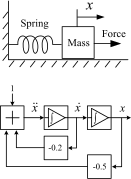
\includegraphics[width=\linewidth]{numerics-ast/AnalogComputerExampleCircuit.pdf}
	\caption[Sketch of a simple analog computing problem.
	\modifiedAfter{AnalogNingPhd}]%
	{Sketch of a damped oscillation as a toy problem from classical mechanics,
		described by the ODE IVP $\ddot x = -0.2 \dot x - 0.5 x + 1$ with ID $x(0), \dot x(0)$.
		The lower panel shows the electrical circuit to solve the \emph{analogue} problem.
		Adopted from \cite{AnalogNingPhd}.}\label{fig:analog-computer}
\end{marginfigure}
While analog computers disappeared from the frontline of computing in favour
of digital computers, even today there is active research stating that analog
computers could solve PDEs in a parallel and energy-efficient way, as it is
out of reach for digital processors \cite{ulmann2013analog}.
It is likely that analog computing will enjoy a similar revival as vector
computing did, in terms of an integration in modern computer generations.
Analog parts could be casted as coprocessors or accelerator
units in the same way as graphic cards and dedicated computing cards are
used today.

In fact, analog models of gravity is a research field on its own
\cite{Barcelo2011,Balbinot:2006ua}, where modern attemps date back to 1980s
proposals of Unruh about accessing black hole evaporation in fluid flows
determined by analog laws \cite{Unruh81}. However, general relativity was not 
solved on analog computers yet, and this remains a research program for the
future.

\section{Time and Space discretizations}
After the excursion of section~\ref{sec:solving-pdes-computers}, for the rest 
of this work, all PDEs are subject to a \emph{numerical} solution (if not 
mentioned otherwise).
This requires to discretize the continuum problem in a suitable way.
The classical literature distinguishes between temporal and spatial
discretization\footnote{
 Where the ``temporal'' direction (dimension) is characterized by the
 (volatile)
 evolution direction while the ``spatial'' directions (dimensions) define
 the spatial simulation domain which is hold in memory.
}.
This section is a short survey in basic grid based methods with focus on
``semi-discrete'' time integration techniques in order to solve PDEs
such as \eqref{intro:ncp}. In contrast, the subsequent
Sections \vref{sec:fv} and \vref{sec:dg} cover fully discrete techniques, \ie
approaches which allow for the PDE solution in a single (uniform) spatial and
temporal discretization procedure.

\subsection{Semi temporal discretization}\label{sec:time-and-mol}
A scheme with spatial discretization, but without a similar
(explicit) temporal one is called \emph{semi discrete}.
Semi discretization is a popular term in literature and may be misleading:
In a numerical attempt to solve PDEs, evventually both the spatial and the
temporal dimensions must be discretized.  However, the different
treatment of the temporal and spatial differential operators as well as the
non-discretization in temporal direction between discrete timesteps
(Figure~\ref{fig:mol})
is a motivation to adopt the term ``semi discrete''.
  
The \emph{method of lines} (MoL) is a particular example of a semi
temporal method. The idea in MoL is 
to recast the PDE describing $u_k(x_i,t)$ into  $n\times N$
ordinary differential equations (ODEs), with $n$ the
state vector length and $N$ the number of points $x_i$ covering the spatial domain
$\Omega$\footnote{
	Note that the MoL approach is invariant under the spatial discretization.
	It does not require any particular grid.
}. That is, the MoL solves one ODE in time (from initial data $t_0$ to $t_1$) 
for every (discretized) spatial point and field, that could be denoted as
\begin{equation}\label{eq:mol-ode}
\partial_t u_k(x_i, t) = \mathcal R(x_i, u_k(t_0), \partial_j u_k(t_0))
\end{equation}
where the spatial differential operator $\mathcal R$ collects all PDE terms
of \eqref{intro:ncp}.
Popular ODE time integrators are Euler's method or the higher order nonlinear
total-variation diminishing (TVD) or 
strong stability preserving (SSP) Runge-Kutta (RK) methods (see
Appendix~\ref{sec:apx-pde-classification} for details). These are explicit
(dependency at time $t$ only on $t_0 < t$, not $t_1 > t$) single-step
(no dependence on $t<t_0$) methods and easy to implement. 
Another popular example for ODE integration are linear multistep high order
integrators, such as the Adams-Bashforth (AB) method which represents the field
with polynomials in time.
The cost to pay for high order methods is the need for repeatedly
evaluate/update the right hand side (RHS) in \eqref{eq:mol-ode},
which requires evaluating spatial
derivatives, which implies communication.

\begin{marginfigure}
	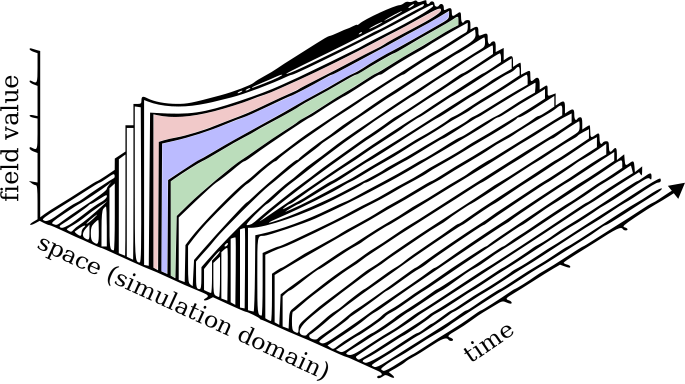
\includegraphics[width=1.05\textwidth]{numerics-mol/mol-motivation.pdf}
	\caption[MOL figure, \colorizedAfter{Schiesser2009}]
	{   Motivation for the naming \emph{Method of Lines}
		\eqref{eq:mol-ode}: The lines are the
		individual solutions at certain positions within the spatial domain,
		over the simulation time. This figure illustrates that space is 
		discretized
		but time is not. The three coloured lines (``slices'' in the 
		height-elevated plot) are neighboured: In order to determine the
		time evolution of the blue slice, information from the green and
		red slice have to be taken into account.
		
		The example shows a scalar diffusion equation $\partial_t \phi = \kappa 
		\partial_x^2 \phi$ 
		with arbitrary $\kappa$ and initial field $\phi_0=\frac 12 
		\exp\left\{-(x-1)^2 
		+ \exp(-(x+1)^2)\right\}$. It is modified and 
		colorized from \cite{Schiesser2009}.
		% Also at english wikipedia: 
		%https://en.wikipedia.org/wiki/Method_of_lines
	}\label{fig:mol}
\end{marginfigure}

Implicit or backward methods such as the Crank-Nicholson are poular for stiff
PDEs due to their small domain of dependency
(\ie the spatial region which influences the solution at a given point due
to causality / characteristic speeds) or for when the timestep size is
constrained by a spatial discretization method (such as in the Discontinous
Galerkin method, see below).
Implicit methods allow larger time\-steps compared to explicit methods. On
the other hand, the solution for a time $t$ has to be found by solving an
implicit equation (\eg iterative root finding).

For special problems, sophisticated time integrators beyond the MoL exist
which take particular problem properties into account. For instance, a
symplectic integrator scheme conserves the momentum space volume $\d p\ \d q$
during the integration of Hamilton's equations by evolving the coupled
canonical coordinates $p$ and~$q$.

\subsection{ADER time integration}
The ADER technique (from \emph{A}rbitrary high order \emph{DER}ivatives) was
pionieered by Toro and Titarev \cite{Titarev2002, Titarev2005, Toro2006}
in the context of Finite volume schemes (Section~\ref{sec:fv}). It
bases on the idea of tayloring the time evolution in~\eqref{eq:mol-ode},
\begin{equation}\label{eq:ader-mol}
\partial_t u_k(x_i, t) = \sum_{l=0}^N \frac{t^l}{l!}
  \partial_t^l u_k(x_i, t_0) \,,
\end{equation}
so that $\Delta t = t-t_0$, and then expressing the $l$th order temporal
derivative with spatial derivatives which are obtained by the PDE weak form
and partial integration with a $N$th order test function, similar as it
will be presented in Section~\ref{sec:dg}. This way, the time update relys on
the $N$th order spatial discretiation and can be computed analytically to $N$th
order.

The ADER approach leads to arbitrary high-order accurate fully discrete one-step
schemes in space and time. The arbitrariness here is just represented by the
fact that $N\in\mathbb N$ can be choosen freely (with bigger $N$ resulting
in higher computational cost, of course). \emph{one-step} effectively means
no repeated evaluation of the \eqref{eq:ader-mol} RHS. This is the
communcation-avoiding property of the ADER approach which pays off on massively
parallel grids.\footnote{
	Appendix \vref{sec:rkdg-performance} compares the ADER time evolution with
	the Runge-Kutta one.
	
}

%\todo{hier komischer Verweis auf Astrophysik-Verewendungen, weiß nicht ob das
%gut ist}
%ADER schemes have already been applied to the
%equations of relativistic MHD, both in the ideal case (see
%\cite{Dumbser2008,Zanotti2015,Zanotti2015d}) and in the
%resistive case \cite{Dumbser2009} and to other nonlinear
%systems of partial differential equations
%\cite{Zanotti2015c,Fambri2017}.

\subsection{CFL factor}
In hyperbolic systems, the temporal discretization is limited by the spatial
discretization. The formalization for limiting the timestep size
$\Delta t = t_1-t_0$ is known as the Courant-Friedrichs-Lewy (CFL) condition.
The argument can easily derived by the classical kinematic law
$s=v\cdot t$, with $s$ the traveled
distance of a particle moving with constant velocity $v$ over time $t$.
Given the distance $\Delta x = \Lambda_i \Delta t$ is traveled by a system's
wave with characteristic (eigenvalue) $\lambda_i$, the maximum timestep is
therefore constrained from above,
\begin{equation}\label{eqn:def-cfl}
\Delta t \leq \Delta x / \Lambda \,,
\end{equation}
with $\Lambda$ the maximum of the systems eigenvalues $\lambda_i$. In practice,
the inequality \eqref{eqn:def-cfl} is replaced by
$\Delta t = C \Delta x / \Lambda$ with $0 < C \leq 1$, where the arbitaryily
chosen $C$ is called the CFL or Courant factor.

\subsection{Methods for spatial discretization}
For spatial discretization, there exist a couple of standard classes with 
different attemps.
While adopting a somewhat regular grid (Figure \ref{fig:fd-stencil-intro}) is
probably obvious (Section \ref{sec:grid-meshing} discusses grid meshing in detail),
there is a whole class of \emph{meshfree} methods. A particular example is
smoothed-particle hydrodynamics (here coordinates move with the fluid), which is
in particular popular in astrophysics, since it easily allows to
cover several orders of magnitude in length scales. Hybrid attemps exist, such
as Particle-in-cell (PIC) approaches which combines particle methods with
grid based ones.

Another general class of methods are \emph{spectral} methods where the simulation
domain $\Omega$ is covered by a function basis \cite{hesthaven2007}.
This is typically used for smooth
problems where Fourier series can be used to eliminate differential operators.
Formally, spectral methods belong to \emph{finite element} methods (FEM) which first
subdividide the computational domain $\Omega$ by a finite number of (typically)
nonoverlapping elements $\Omega_i$ where the spectral methods are then applied
within (see also Section~\ref{sec:dg-subcell-structure}). 
Finite-element methods are
known also under the name of {variational-difference} or
{projection-difference} methods \cite{Ritz1909,Galerkin1915}.

\emph{Finite volume} methods (FVM or just FV) share some features with FEM,
and these two terms can be used in some respect synomyously, whereas ``FEM''
has a slight focus on meshing topologies and embedding of methods within
single cells, while ``FVM'' has to some extend a focus on the integral
formulation and interfacing of cells (Godunov's method, Riemann problem),
typicall implemented around a grid with small volumes around spatial points.

A clear distinction however can be made between FV and \emph{finite 
differences} (FD) methods. In the later method, the PDE is solved by employing
the finite difference quotient between certain connected points in a grid,
while a FV scheme works on volume and surface integrals, applying Gauss'
theorem.

\subsection{Finite-difference schemes}
\begin{marginfigure}[-4cm]
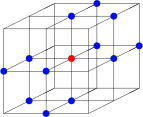
\includegraphics[width=\linewidth]{numerics-schemes/FD-Stencil-3d.pdf}
\caption[
  FD stencil motivational cartoon, \colorizedAfter{FDStenicl3d} 
]{
  Example of an arbitrary three dimensional finite differencing stencil.
  Dependent points (blue) are neighbouring the evaluation point (red).
  In order to compute the derivative of a field on this grid at the red point,
  all dependent points in a certain direction projection are taken into account.
  (coloured from \cite{FDStenicl3d})
}\label{fig:fd-stencil-intro}
\end{marginfigure}

Finite differencing is probably the most straightforward way of solving
differential equations on a computer. The starting point and origin of
the name is to undo the infinite limit $h\to\infty$ of the difference quotient
\begin{equation}
\dd{f(x)}{x} \approx \frac{f(x+h) - f(x)}{(x+h) - x}
\end{equation}
By choosing a finite but small $h$, the spatial differential operator in the
Method of Lines \eqref{eq:mol-ode} can be computed. The most simple way to
implement this is to discretize space on a finite number of grid points
$x_i = i\Delta x$, store the
function values $f(x_i)=f_i$ and set $h=\Delta x$.

The concept is easily extended to generic finite differencing stencils
(Figure~\ref{fig:fd-stencil-intro}),
higher dimensions and arbitrary order derivatives ($\d f/{\d^n x}$).
%Adopting finite differencing codes for solving hyperbolic conservation laws
%have a long tradition.
Finite differencing techniques are popular for being computationally cheap
and easy to implement. For instance, there is no need to cast a PDE system
into a particular form (such the nonconservative form \eqref{intro:ncp}) and
rectangular regular grids as well as differential stencils
can be represented by (continous storage) arrays.

\begin{marginfigure}[-2cm]
\includegraphics[width=\linewidth]{ghost-cells-ratio/ghost-cell-ratio.pdf}
\caption[
  Sketch of the ghost cell ratio to payload ratio, \exclusive
]{
  Ghost cell volume $G=12xw^2 + 6x^2 w + 8w^3$ to actual physical
  domain $V=x^3$ ratio $R=G/V$ in three dimensions for
  different ghost layer widths $w$ (\ie half the stencil sizes in FD context).
  On the abscissa, the width $x$ of a cuboid (domain or patch) is given in
  number of cells. These small patches are realistic in the
  \code{ExaHyPE} AMR code, while traditional codes such as \code{Cactus}
  have an order of magnitude larger cells.
}
\label{fig:ghost-cell-ratio}
\end{marginfigure}

A major drawback of obtaining high order in a large simulation is the
appearance of \emph{ghost points} outside the simulation domain. In a naive
cartesian domain decomposition for the parallel evaluation of the
differential operator, the ``ghost halo'' fraction can quickly make a
substantial part of the simulation domain on the computer which is especially
costly when it comes to data exchange in the boundary
(Figure~\ref{fig:ghost-cell-ratio}).%

A numerical drawback of high order finite differencing schemes is the 
unsuitability for discontinous solutions where the large stencil will generate
spurious solutions. This makes them unattractive for nonlinear conservation
laws. On the other hand, such problems do not occur in linear and linearly
degenerate systems\footnote{In section \vref{sec:fo-ccz4} it will be shown
that parts of a  particular formulation of Einstein equations, the CCZ4
equations, can be written in a linear degenerate way.} where no shocks can be 
generated if the initial data is not discontinuous itself.

Finite difference methods can be ``fortified'' with a number of methods such
as \emph{artificial dissipation} for stabilisation \cite{Kreiss73}.
Another typical choice
for hyperbolic conservation laws are special \emph{upwinding} stencils to
correctly track the system characteristics. Both topics are typically
covered by Riemann solvers in FV schemes and implementing them explicitely
in FD schemes can be seen as a hardening of the simple FD schemes in order
to gain robustness by maintaining a computationally and logically cheap scheme.
In the same way, FD can also be used empowered
with high resolution shock capturing (HRSC) techniques.
\todo[color=green]{
  FD schemes: There are many details which could be added, such as dissipation
  stencils; citations about Upwinding, HRSC, etc.
}

% Further papers:
%          FD in NR \cite{Baumgarte2010,Bona2009}
%          interesting outlook: Compact finite differences \cite{Lele92}

\section{Finite-volume schemes}\label{sec:fv}
\begin{marginfigure}[2cm]
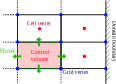
\includegraphics[width=\linewidth]{numerics-schemes/FV-Cells.pdf}
% Roughly inspired by 
% \url{http://arturo.imati.cnr.it/~marco/Research/Finite_Volumes/index.html}
\caption[
   Cartoon of a Finite Volume description, drawn with Inkscape, \exclusive
  ]%
  {Finite volume simulation domain and termiology in an exemplaric simple
   two-dimensional Cartesian grid with rectangular cells. Shown are the cell
   barycenters, the cell corners, a domain boundary, the fluxes/waves which
   are described by the Riemann problem for a single highlighted
   demonstrator cell.
}
\end{marginfigure}

Finite-Volume schemes discretize the simulation domain $\Omega$
into cells $\Omega_i$ which shall hold \emph{cell averaged} or
\emph{piecewise constant} solutions. It was the insight of Godunov
in 1959 \cite{Godunov59} to solve then the Riemann problem (Section~\ref{sec:riemann-problem})
at these interfaces in order to solve the PDE. Godunov's method itself is
fully discrete in time and space, but its time update can easily be replaced
by the method of lines (Section~\ref{sec:time-and-mol}).
%With this approach, the problem of
%solving the RHS of MOL reduces to the interfaces $\partial\Omega_i$
%between these cells and it was the insight of Godunov in 1959 to solve the
%Riemann problem at these interfaces
For recent reviews for FV in relativistic astrophysics, see \cite{Font08,Marti03}.

\subsection{Godunov's scheme}
A finite volume scheme works on the average value $\u^n_i$ of the state vector within
a spacetime-cell $[t^n, t^{n+1}] \times \Omega_i$, and for simplicity we work in
one dimensions in this subsection, so $\Omega_i=[x_i, x_{i+1}]$,
$\Delta t = t^{n+1} - t^n$ and $\Delta x=|\Omega_i|=x_{i+1}-x_{i}$. The cell barycenter is located at $x_{i+1/2} = x_i + \Delta x/2$ and the cell average given by
\begin{equation}
\label{eqn.subcellaverage}
\bar \u^n_i := \frac{1}{|\Omega_i|} \int \limits_{\Omega_i}
\u(t^n,x)  ~\d x
\,.
\end{equation}
Godunov's scheme can be derived by integrating the PDE \eqref{intro:ncp}
in time and applying the piecewise constant assumption $\u(t,x) \equiv \u_i^n$
for $t\in[t^n,t^{n+1}]$. The time integral collapses and allows to write
\begin{equation}\label{eq:godunov}
\u^{n+1}_i = \u^n_i - \frac{\Delta t}{\Delta x}
   \left(\boldsymbol f_{i+1/2} - \boldsymbol f_{i-1/2} \right)
   + \frac{\Delta t}{\Delta x} \boldsymbol B \cdot
   \left( \u^n_{i+1/2}  - \u^n_{i-1/2} \right)
   + \Delta t \boldsymbol S(\u^n_i)
   \,.
\end{equation}
Here, a couple of remarks are neccessary: First, this scheme is obviously
fully discrete in space and time, as well as explicit in time. The conserved
flux was replaced by a numerical flux which is thanks to the piecewise
constant assumption just given as
%Analytically the numerical flux is a time integral over the cell surface,
%\begin{equation}\label{eq:godunov-flux-integral}
%\boldsymbol f_{i\pm 1/2} =  \int\limits_{t^n}^{t^{n+1}} \frac{\d t}{\Delta t} \boldsymbol F(\u(t,x_{i\pm 1/2}))
%\end{equation}
%however,allows the integral \eqref{eq:godunov-flux-integral} to collapse and the fluxes
%to be given just as
\begin{equation}
\begin{aligned}
\boldsymbol f_{i - 1/2} &= 
 \frac 12 \left(
 \boldsymbol F(\u^-_{i-1/2}) + 
 \boldsymbol F(\u^+_{i-1/2})
 \right)
&&=
\frac 12 \left(
   \boldsymbol F(\u^n_{i-1}) + 
   \boldsymbol F(\u^n_{i})
\right) \,,
\\
\boldsymbol f_{i + 1/2} &= 
\frac 12 \left(
 \boldsymbol F(\u^-_{i+1/2}) + 
\boldsymbol F(\u^+_{i+1/2})
\right)
&&=\frac 12 \left(
\boldsymbol F(\u^n_{i+1}) + 
\boldsymbol F(\u^n_{i})
\right) \,.
\end{aligned}\label{eq:godunov-riemann-trivial}
\end{equation}
Second, since Godunov's method is first order, the nonconservative contribution
vanishes as the boundary extrapolated data are equal, $\u^n_{i+1/2}  - \u^n_{i-1/2}=0$.
The nonconservative source term $\boldsymbol B$ therefore vanishes.

The essential idea of Godunov is now that with the piecewise constant assumption,
a Riemann problem can be solved at each cell interface. The initial data for the
Riemann problem between $x_{i}$ and $x_{i+1}$ is then given by the two cell values
\begin{equation}\label{eq:godunov-riemann-interface}
\u(t^n,x) = \u^n_i \theta(x-x_{i+1/2}) + \u^n_{i+1} \theta(x_{i+1/2}-x)
\end{equation}
with Heaviside step function $\theta(z)$.
Once the Riemann problem is solved, also
the the time update \eqref{eq:godunov} is given
\footnote{
 The CFL conditions \eqref{eqn:def-cfl} must be fulfilled and the scheme can be
 easily extended to higher dimensions in a dimension-by-dimension fashion.
}. We call equations of type
\eqref{eq:godunov-riemann-trivial} Riemann solvers and in fact this simple one
is already sufficient for first order Godunov. However, there are more sophisticated
Riemann solvers which do not make the piecewiese constant assumption. 
Popular choices are the Roe solver and HLLE solver (see next Sections).

\subsection{Higher order finite volume}
\begin{marginfigure}
	\centering
	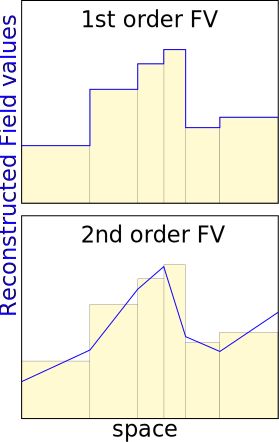
\includegraphics[width=0.88\linewidth]{exahype-2nd-order-fv-gridstructure/high-order-reconstruction.pdf}
	\caption[FV Higher order reconstruction, Cartoon drawn with Inkscape, 
	\exclusive]%
	{Cartoon which demonstrates how higher order reconstruction of the field
	 works: While a first order reconstruction method assumes cells to have
	 an average value (cells in this one-dimensional example are non-uniformly
	 sized), in a second order reconstruction (think of a Taylor expansion in
	 each cell, with a linear term) the field is approximated by taking
	 neighbouring cells into account. In general, requirements such as a
	 continuity condition do not neccessarily have to be fulfilled, while
     they typically are desirable in schemes.
     }
	\label{fig:higher-order-reconstruction}
\end{marginfigure}
Higher order FV is archieved by improving description of the interface
state values $\u^{\pm}$ by taking next-to-neighbour cells into account. 
The simplest
possibility is to switch to a piecewise linear 2nd order description
where $\u_i(x) = \u_i + v_i(x-x_i)$ within a cell 
(Figure~\ref{fig:higher-order-reconstruction}).

TVD conditions lead to non-linear limiting of slopes, such as the minmod limiter.
In general, a $k$th order reconstruction operator
\begin{equation}
\mathcal R\left[ \q_i \right] = \lim_{y \to x_i} \q(y) + \mathcal O(\Delta x^k)
\end{equation}
applied at a cell average at position $x_i$ reconstructs the continous field $\q$
locally around $x_i$. Successful methods used in the literature are for
instance the
piecewiese parabolic method (PPM), the essentially non-oscillatory (ENO),
the weighted essentially non-oscillatory (WENO) and the monotonicity-preserving 
(MP) \cite{Radice2012b}.
All of them are high resolution shock capturing, \ie they preserve a good resolution
at discontinuities and do not introduce spurious oscillations.

Similar as to FD methods, for a $k$th order reconstruction, the domain of dependency
includes $k$ neighbouring cells per dimension. Reconstruction operators can also be
formulated in stencils which look like FD stencils.

\subsection{Riemann solvers and the nonconservative 
product}\label{sec:riemann-nonconservative}
The generic integral form for solving \eqref{intro:ncp} with FV introduces a space
and time integral,
\begin{fullwidth}
\begin{equation}
\label{eqn.fv.generic}
\boldsymbol{u}^{n+1}_{i} - \boldsymbol{u}^{n}_{i} 
%
- \iint \limits_{T^n ~ \partial\Omega_i}
\mathcal F(\q^-,\q^+)
\,\mathrm d^d x\,\mathrm dt
= \iint \limits_{T^n ~ \Omega_i}
\left[\boldsymbol S(\q) - \boldsymbol{B}(\q) \cdot \nabla \q  \right]
\,\mathrm d^d x\,\mathrm dt
\,.
\end{equation}
\end{fullwidth}
Here, $\mathcal F$ is the numerical flux at the element interface. If not mentioned
otherwise, a simple Rusanov Riemann solver is used \cite{Rusanov1961a},
\begin{fullwidth}
\begin{equation}
\mathcal{F}\left(\q_h^-, \q_h^+ \right) \cdot \boldsymbol{n} = \frac{1}{2}
\left( \boldsymbol{F}(\q^+) + \boldsymbol{F}(\q^-) \right) \cdot \boldsymbol{n}
- \frac{1}{2} |\Lambda_i| \left( \q^+ - \q^- \right) \pm \frac 12 \boldsymbol 
B\left( \frac{\q^+ + \q^-}2 \right)
\cdot \boldsymbol{n} \left( \q^+ - \q^- \right)\,.
\label{eq:rusanov}
\end{equation}
\end{fullwidth}
Note that for the piecewise constant approximation (Godunov's first order scheme),
$\q^+ = \q^-$ and \eqref{eq:rusanov} reduces to 
\eqref{eq:godunov-riemann-trivial}.

It should be stressed that the use of the nonconservative product within the
Riemann solver/path conservative integration is \emph{not} required per-se.
It would have been equally possible to integrate a differential source in a
non-path conservative way. However, the special treatment allows it to formulate
well-balanced numerical methods \cite{Bermudez1994}. 

%\todo{Important: Move NCP discussion from ADER-DG scheme to this point}
The inspiration to use {path-conservative} schemes for
nonconservative products has been taken from successful developments in
the context of  {well-balanced} numerical methods
for the solution of the shallow-water equations 
\cite{Pares2006,Castro2006,Castro2010},
where the bottom-slope term (which is the gradient of a known
function and accounts for gravitational forces in shallow-water models) is 
discretized as a nonconservative product in the principal part of the
system rather than as a classical algebraic source term. In the shallow
water context, the family of path-conservative schemes allows to preserve
certain stationary equilibrium solutions {exactly} up to machine
precision also on the discrete level, including nontrivial equilibria
\cite{Gaburro2017,Gaburro2018}.


%In the following, a MUSCL TVD scheme as well as a WENO shall be presented in detail,
%as they are implemented in ExaHyPE.

\subsection{MUSCL-Hancock}\label{sec:MUSCL}
\begin{marginfigure}[3cm]
	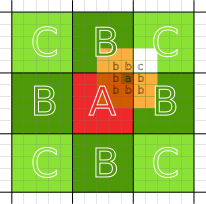
\includegraphics[width=\linewidth]{exahype-2nd-order-fv-gridstructure/exahype-2nd-order-fv-gridstructure.pdf}
	\caption[2nd order FV ExaHyPE ghost cell problem, drawn with Inkscape, 
	\exclusive]%
	{
       Cartoon of the ghost cell optimization in \code{ExaHyPE}:
       Patches are denoted with upper case letters ($\mathbb A$, $\mathbb B$,
       $\mathbb C$), while embedded FV subcells are denoted with lowercase
       letters ($\mathbb a$, $\mathbb b$, $\mathbb c$). The letter $a$ refers
       to the patch/cell which solution shall be computed. The letters $b$
       refer to their direct neighbours (sharing a face), while the letters
       $c$ refer to the corners (sharing an edge).
       Two ghost layers are drawn.
       Here, the information in the domain $\mathbb C \cap \mathbb c$ is
       not available.}\label{fig:muscl-exahype}
\end{marginfigure}

The second-order acurate MUSCL-Hancock TVD finite-volume scheme
\citep{toro-book} is the second-order FV scheme available in
\code{ExaHyPE}. It has proven robustness in the presence of
shock waves and low density atmospheres. 
Formally, the second-order MUSCL-Hancock scheme can be derived from the PDE
\eqref{intro:ncp} as in \eqref{eqn.fv.generic}.

High order in space, together with non-oscillatory properties, are
achieved  via a {nonlinear} reconstruction of
piecewise polynomials from the known cell averages
$\bar{\boldsymbol{v}}_{i,s}^n$ using a TVD reconstruction. In order to
preserve high resolution shock capturing properties, high order
reconstruction requires slope limiting (also refered to as flux limiting).
Such a limiter allows to restrict the order of the scheme at discontinuities.
In \code{ExaHyPE}, different slope limiters were implemented, such as the
\emph{minmod} \cite{Roe86} or the \emph{Koren} limiter~\cite{Koren1993}.

Particulary relevant for \code{ExaHyPE} is the fact that in this code,
the reconstruction stencils at patch boundaries lack isentropy
(Figure~\ref{fig:muscl-exahype}).
In \code{ExaHyPE}, corner cells are not synchronized for performance reasons
(especially because it is primarily a DG code and DG does not require
the knowledge of corner values). This requires the FV reconstruction in
$d\geq 2$ dimensions to stick to a $+$ shaped stencil at the corner
(domain $\mathbb A \cup \mathbb B$ or $\mathbb a \cup \mathbb b$ in Figure
\ref{fig:muscl-exahype}), \ie the field information $\mathbb c$ is not
available, while $\mathbb B$ and $\mathbb b$ is.
For slope limiting, a conservative estimate (guess) on the slopes has to be
made.
The problem does not occur in a first order scheme where no
reconstruction takes place.

\subsection{WENO}

As an alternative to the MUSCL scheme, an arbitarily accurate ADER-WENO
finite-volume schemes can be used in the \code{ExaHyPE} prototype.
The weighted essentially non-oscillatory (WENO) approach does not clip local
extrema, in contrast to the second-order TVD method. For fluid dynamics
(Chapter~\ref{chapter:hydro}) the TVD scheme was found to be more robust
than the WENO scheme.

The (ADER-) WENO scheme scheme shares many aspects of the (ADER-) DG
schemes presented in the subsequent Section~\ref{sec:dg}. The spacetime
predictor solution $\q_h$ is however computed from an initial
conditition given by a WENO reconstruction polynomial $\w_h(\x,t^n)$
computed from the cell averages
$\bar{\u}^n_{i,s}$ via a multi-dimensional WENO reconstruction operator
detailed in \cite{Jiang1996,Dumbser2008,Dumbser2013}. The values at the cell
interfaces $\q_h^-$ and $\q_h^+$ are computed as the boundary
extrapolated values from the left and the right subcell adjacent to the
interface.

The nonlinear WENO reconstruction works as follows: for each subcell
$\Omega_{i,s}$ we compute several reconstruction polynomials
$\w_h^k(\x,t^n)$ requiring integral conservation of $\w_h^k$ on a set of
different reconstruction stencils $\mathcal{S}^k_{i,s}$,% \ie
\begin{equation}
\frac{1}{|\Omega_{i,j}|} \int \limits_{\Omega_{i,j}} \w^k_h(\x,t^n)
d \x = \bar{\u}^n_{i,j} \qquad \forall \, \Omega_{i,j} \in
\mathcal{S}^k_{i,s}\,.
\end{equation}
This system is solved via a constrained least-squares algorithm requiring
at least exact conservation in the cell $\Omega_{i,s}$ itself 
\cite{Dumbser2007b}. From the set of reconstruction
polynomials $\w_h^k$, the final WENO reconstruction polynomial $\w_h$ is
obtained by using a classical nonlinear weighted combination of the
polynomials \cite{Jiang1996,Dumbser2007b}
%
\begin{equation}
\label{eqn.weno}
\w_h(\x,t^n) = \sum \limits_k \omega_k \w_h^k(\x,t^n),
\quad \textnormal{with} \quad \omega_k = \frac{\tilde{\omega}_k}
{\sum \limits_l \tilde{\omega}_l}
\quad \textnormal{and}  \quad \tilde{\omega}_k = \frac{\lambda_k}
{(\sigma_k + \epsilon)^r}\,,
\end{equation}
%
where the oscillation indicators $\sigma_k$ are computed from
%
\begin{equation}
\sigma_k := \sum \limits_{l\geq 1} \int \limits_{\Omega_{i,s}}
\Delta \x_{i,s}^{2l -1} \left( \frac{\partial^l}{\partial \x^l}
\w_h^k(\x,t^n) \right)^2 d \x\,.
\end{equation}
%
The small parameter $\epsilon$ in \eqref{eqn.weno}, which is only
needed to avoid division by zero, is typically set to $\epsilon=10^{-14}$
and the
exponent in the denominator is chosen as $r=8$. The linear weights are
$\lambda_1 = 10^5$ for the central stencil (\ie $k=1$), while all other
stencils (\ie $k>1$) have linear weight $\lambda_k=1$. This choice
corresponds also to the one made in \cite{Dumbser2007b}.

In a practical implementation it is convenient to write also the
WENO reconstruction polynomials in terms of some reconstruction basis
functions $\psi_l(\x)$ as $\w_h(\x,t^n) = \Psi_l(\x) \hat{\w}_l^n$. 
Here, following \cite{Dumbser2008}, the basis functions $\Psi_l$
are defined in the same way as the $\Phi_l$ in Section~\ref{sec:dg-subcell-structure},
\ie as tensor products of Lagrange
interpolation polynomials through the Gauss-Legendre quadrature
nodes. %For the limiter, we only use a piecewise quadratic reconstruction,
%leading to a nominally third-order accurate scheme. As already mentioned
%before, the predictor is computed according to \eqref{eqn.pde.st2}, where
%the initial data $\u_h(\x,t^n)$ is replaced by $\w_h(\x,t^n)$ and the
%spatial control volumes $\Omega_i$ are replaced by the subcells
%$\Omega_{i,s}$.

\section{Discontinous Galerkin schemes}\label{sec:dg}
\begin{marginfigure}[-4cm]
  \includegraphics[width=\textwidth]{dg-fv-intro-sketch/fileformat-sketch-cont.pdf}
  \includegraphics[width=\textwidth]{dg-fv-intro-sketch/fileformat-sketch-discont.pdf}
  \caption[
    1D DG Motivational example, Matplotlib sketch, 
    \publishedIn{exahype-guidebook}
  ]{A motivational cartoon of DG in one dimensions: A $N=2$ polynomial
    with $N+1$ DOF ($a+bx+cx^2$) is embedded in each cell. The cell sizes and
    nodal basis points (red) are arbitrary in this plot and in general. The
    shading indicates the single cell averages (one DOF). The upper panel shows
    a continuous function while the lower panel shows an example with 
    jumps/discontinuities at the cell interfaces, yielding in a double valued
    function at the cell interface. In contrast to high order FV, the DOF
    really live within a single cell and no reconstruction takes place which
    averages over multiple cells.}
  \label{fig:dg-motivational-sketch}
\end{marginfigure}

Galerkin methods (developed independently by Boris Galerkin and Walther Ritz,
but named only after Galerkin)
are another method to discretize a PDE, by casting it in a weak (integral)
formulation
where test function and solution are part of a Hilbert space. A finite
discretization is then achieved by the approximative projection to a
finite-dimensional Hilbert space; a matrix representation instead is achieved
by finding an orthogonal basis in this function vector space. Formally this
class of methods bear resemblance to spectral methods and can share the same
properties such as exponential convergence. Thus Galerkin methods are formally
finite element methods which combine the advantages of spectral methods with
grid-based methods.

Discontinous Galerkin (DG) schemes then again combine Galerkin methods with
Finite Volume paradigms (Godunovs methods). DG methods can be motivated as
an extension to FV methods where a single cell average is replaced by more
degrees of freedom, such as a linear or quadratic approximation of the real
solution. As the particular feature, the approximations between the cells
don't have to be smooth/continous but can exhibit jumps
(Figure~\ref{fig:dg-motivational-sketch}). Of course, in the continuum limit
where the cell size goes to zero while the number of cells goes to infinity,
these discontinuities are as well defined as the discontinuity of Godunovs
piecewise constant method itself.

Given the concept of embedding information within a cell (or patch), DG methods
exhibit $hp$-adaptivity: Meshes can be refined both in terms of cells
($h$-refinement) or in terms of subcell degrees of freedoms ($p$-refinement).
For classical grid $h$-refinement, DG methods exhibit polynomial accuracy
(similar to FV/FD), while for subcell $p$-refinement they exhibit spectral
accuary.

In DG methods, the number of degrees of freedom $p$ is naturally associated to
the order of the scheme. A major benefit of DG schemes is the need of only one
ghost layer \footnote{
  Since DG uses a polynomial basis, the concept of an integral number of
  ``layer cells'' (as in FD/FV) makes no sense. One ghost layer means, that
  the field values on the lower-dimensional surface of the computational domain 
  need to be exchanged within the corrector phase of the scheme presented
  in Section~\ref{sec:holy-dg-scheme}. In a two dimensional simulation on
  square elements, the one dimensional polynomials on four element border lines
  have to be exchanged. In a three dimensional simulation on cuboid elements,
  the two dimensional polynomials on six element surfaces have to be
  exchanged. No particular treatment is neccessary for the edges/corners of
  the squares/cuboids.
} at any order, due to the functional basis within one cell. That
provides optimal scalability and makes DG attractive for large parallel 
problems,
in fact explains the spreading of DG methods in the Exascale era. The price
which has to be paid (in comparison to a FV scheme) is primarily the complexity
of an implementation which cannot be underestimated. The DG method will get
intertwined with the way how the grid is managed and how communication works.
Arguable disadvantges of the DG method (compared to a FV method) are its
apparently larger memory footbringt, coming from the larger amounts of degrees
of freedom and, for explicit DG methods, the limitation on the timestep size (a
penalty of $\sim 1/2N$
where $N$ is the degrees of freedom, compared to a FV method). However, this
criticism disregards the high order spectral convergence which allows to
describe smooth problems with orders of magnitudes less cells then any high
order FV method would allow to. A way to alleviate the severe CFL timestep
restriction is the use of semi-implicit DG schemes, as those proposed, for
instance by \cite{Tavelli2016,Fambri2016}.

DG methods have been proven to be non-linearly stable at all orders and can
be formulated covariantly~\cite{meier_1999_mas}. Similar as Godunovs method, the
mathematical foundations are only well defined for first order PDEs,
but DG has been applied to second order PDEs.

It has taken nearly two decades for the DG methods to be
extended to general nonlinear hyperbolic systems, thanks to the
groundbreaking works of \cite{Cockburn1989b,Cockburn1990,CockburnShu98}.
DG methods are reviewed in 
\cite{cockburn_2000_dg,cockburn_2001_rkd,Shu2016,hesthaven2007,hesthaven2008,Cockburn2003}
whereas \cite{ADERNSE,Dumbser2009,Dumbser2010b} provide the fundaments
for the path-conservative nodal semi-discrete ADER-DG methods which are
presented in the following.
%

\subsection{Subcell structure in nodal DG schemes}\label{sec:dg-subcell-structure}
In order to mathematically describe the DG structure, a couple of symbols
shall be introduced. The
computational domain $\Omega$ is fully covered by a finite number $N_e$ of 
non-overlapping elements $\Omega_i$, also referd to as \emph{patches} or 
\emph{cells}  \cite{Khokhlov98}. Especially
the usage of the term \emph{cells} stresses the close relationship to FV 
methods. 
In $d$ spatial dimensions, the cells are characterized by their individual size
$\Delta \vec x_i \in \mathbb R^d$
and barycenter $\vec x_i \in \mathbb R^d$.
%
The discrete solution (state vector of the PDE) is denoted by
$\boldsymbol{u}_h$ and is defined in the space of tensor products
of piecewise polynomials of degree $N$ in each spatial direction,~\footnote{
 	To clarify:
 	$\boldsymbol u$ is the analytic solution while $\boldsymbol u_h$ is
 	an approximation within the restricted space of solutions which
 	can be represented by piecewise polynomials.
 	
 	Furthermore, for the sake of a readable notation, vector indices are
 	now neglected in favour of discrete indices and flags.
 } 
\begin{equation}
\boldsymbol{u}_h(\boldsymbol{x},t^n) = \sum \limits_l \hat{\boldsymbol{u}}_{i,l}
\Phi_l(\boldsymbol{x}) := \hat{\boldsymbol{u}}_{i,l}^n \Phi_l(\boldsymbol{x})\,.
\label{eqn.ansatz.uh}
\end{equation}
Here, obviously the spatial basis functions
$\Phi_l(\boldsymbol{x})$ spawn the
orthogonal $N^d$-dimensional function vector space $\mathcal{U}_h^N$. In 
$\mathcal{U}_h^N$,
$\boldsymbol u$ has the components $\hat{\boldsymbol u_l}$ in each direction
$l\in \mathbb N^d$. $\hat{\boldsymbol u_l}$ are the discrete components/degrees
of freedom of the solution which have to be stored.

The spatial basis functions $\Phi_l(\boldsymbol{x}) = \prod_{i=1}^d 
\varphi_{l_i}(\xi_i)$ are generated by the one-dimensional
basis functions $\varphi_k(\xi)$ on a one-dimensional reference element with
normal extend $\xi\in[0,1]$. The physical coordinates $\boldsymbol x\in\Omega_i$
are mapped to the reference coordinates $\boldsymbol \xi\in[0,1]^d$ by
\begin{equation}
\boldsymbol{x} =
\boldsymbol{x}_i - \halb \Delta \boldsymbol{x}_i + \boldsymbol \xi
\cdot \Delta \boldsymbol x
\,.
\end{equation}
\begin{marginfigure}
	\includegraphics[width=\textwidth]{aderdg-subcell-grid-tikz/gauss-lagrangue-grid.pdf}
	\caption[
	  Gaussian quadrature nodal basis examples, TikZ figure,
	  \ownPub{Dumbser2017}.
	]{Some Gaussian quadrature nodal basis on the one-dimensional reference cell.
	  These two examples have been implemented in the \code{ExaHyPE} code.}
	\label{fig:guass-lagranguage-grid}
\end{marginfigure}
In order to apply Gaussian quadrature, typically Legendre polynomials are used
for the basis functions $\varphi_k(\psi)$ and $\xi_i$ shall be the quadrature
nodes of the $(N+1)$ point Gauss quadrature formula. The Gauss-Legendre 
quadrature has the advantage of a diagonal mass matrix \footnote{
  The mass matrix is defined as $M_{ij}=\int \Phi_i(x) \Phi_j(x) \d x$.
  An extensive discussion of the consequences of a non-diagonal Mass matrix and
  especially of Gauss Legendre vs. Gauss Lobotto in AMR codes is given
  in~\cite{Teukolsky2014MM}.
}. The cost to pay is a non-uniform
nodal basis (subcell grid structure), especially there is no nodal point at the
cell boundary\footnote{This hides the double valued character of the field
 value at the patch boundary at the first glance, for instance when no polynomial
 reconstruction is done in a naive (Gauss-Legendre) vertex-interpolating
 visualization, as typically done when vizualizing DG results.}.
In our implementation we also support the Gauss-Lobatto
quadrature with its uniformly distributed nodal points. In this basis, there are
always points on the cell boundary (Figure~\ref{fig:guass-lagranguage-grid}).
The actual nodal basis is a pure technical decision and (except for the
quadrature rule) has no impact on the mathematical structure of the scheme,
therefore we assume the Legendre nodes in the following exposition whenever
in doubt. \footnote{
See also \cite{stroud}
for a detailed discussion of multidimensional quadrature.
}

The orthogonal polynomials satistfy the interpolation property
$\varphi_k(\xi_j) = \delta_{kj}$. Thanks to this nodal tensor product basis, 
the entire subsequent scheme can be written \emph{dimension for dimension}, all
higher-dimensional
integrals decompose in a multiplication of one-dimensional integrals which
can be evaluated on $N+1$ DOF in each dimension. 

To summarize, note again that the
total number of quadrature points $\{\x_{\text{GP}}^m\}$ in
$\Omega_i$, as well as the total number of basis elements $\{ \phi_k\}$,
is $(N+1)^d$.

%=============================================================
\subsection{A path-conservative ADER-DG scheme}\label{sec:holy-dg-scheme}
%=============================================================
The weak formulation of a first order PDE system \eqref{intro:quasi-linear} is
recast as integral equation by integrating over the control volume
$\Omega_i \times [t^n, t^{n+1}]$,
%\todo{Probably bring unter somewhere:
%This scheme is developed by the Trento group and presented in various
%papers such as \cite{Zanotti2015c,Zanotti2015c,Zanotti2015d,ADERDGVisc}
%in the context of the Euler equations of compressible
%gas dynamics, ideal MHD, special relativistic RMHD, compressible
%Navier-Stokes and viscous and resistive MHD equations.
%}%
%
\begin{equation}
 \int \limits_{t^n}^{t^{n+1}} \int\limits_{\Omega_i } \Phi_k \left[
  \partial_t \boldsymbol{Q} + \boldsymbol{A}(\boldsymbol{Q}) \cdot\nabla
  \boldsymbol{Q}
  -\boldsymbol S (\boldsymbol Q)
  \right] \,\mathrm d^d x\,\mathrm dt = 0\,, \label{eq:weakPDE}
\end{equation}
%
where $\Phi_k\in \mathcal{U}_h^N$ is a generic basis element out of the
piecewise polynomials of maximum degree $N$ which are by definition allowed
to be discontinous across the element interfaces $\partial \Omega_i$. The
resulting jump terms have to been properly taken into account.
This is done in our
numerical scheme with the aid of the path-conservative approach, first
developed by Castro and Par\'es in the finite-volume framework
\cite{Castro2006, Pares2006} and later extended also to the DG
finite-element framework in \cite{Rhebergen2008, Dumbser2009a,
	Dumbser2010}.
In this ADER-DG framework, higher order in time is
achieved with the use of an element-local space-time predictor, denoted
by $\boldsymbol{q}_h(\boldsymbol{x},t)$, which is subject to later discussion.
At this point of the deviation, the solution $Q$ will just be replaced by the
local predictor solution $\boldsymbol{q}_h=\Phi_k(\boldsymbol{x}) \boldsymbol{\hat u}^n_k$.
By integration of the first part in time, and adding a surface flux integral for
the integral over system matrix $\boldsymbol A$\footnote{
  A similar flux is not even possible for the source $\boldsymbol S$
  because it is by construction purely algebraic and must lack derivatives.
}, thus taking jumps between elements into account,
the approximation to the weak form solution \eqref{eq:weakPDE} can be written as
%
\begin{fullwidth}
\begin{align}
\label{eqn.pde.nc.gw2}
\left( \hat{\boldsymbol{u}}^{n+1}_{i,l} - \hat{\boldsymbol{u}}^{n}_{i,l} 
\right)
\int \limits_{\Omega_i}  \Phi_k \Phi_l \,\mathrm d^d x
%
+ \iint \limits_{T^n ~ \Omega_i^\circ}
 \Phi_k \left( \boldsymbol{A}(\q_h) \cdot \nabla \q_h  \right)
 \,\mathrm d^d x\,\mathrm dt
+ \iint \limits_{T^n ~ \partial \Omega_i}
 \Phi_k \mathcal{A}\left( \q_h^-, \q_h^+ \right)
 \cdot \boldsymbol{n} 
 \,\mathrm d^{d-1} x\,\mathrm dt
=
\iint \limits_{T^n ~ \Omega^\circ_i}
\Phi_k \boldsymbol{S}(\q_h)  
 \,\mathrm d^d x\,\mathrm dt
\,,
\end{align}
\end{fullwidth}
%
where the first integral is a scalar product between two basis elements
(called ``element mass matrix'', diagonal for the Legendre basis nodes), the
second integral collects the smooth part of the discrete solution in the
interiour $\Omega_i^\circ = \Omega_i \backslash \partial \Omega_i$\footnote{
  The volume integrals $\int_{\Omega^\circ}$ can be
  evaluated exactly in $N$th order with Gaussian quadrature, since all functions
  under the integral are written on the $(N+1)$th nodal basis.	
}, the third
integral collects the unsteady solution across element interfaces on the
surface $\partial\Omega$ and the fourth integral is the source term volume
integral which unterwent no special treatment thanks to the purely algebraic
nature of the source terms (lack of derivatives).

In order to distinguish the conservative and nonconservative fluxes, the
weak form \eqref{eq:weakPDE} shall be expanded again, this time by using
the PDE functions $F^i_j$ and $B^{ij}_k$ in
$\boldsymbol A = \partial \boldsymbol F / \partial \boldsymbol Q + \boldsymbol B$,
%
\begin{fullwidth}
	\begin{equation}
	\begin{aligned}
	\label{eqn.pde.nc.gw3}
	\left( \hat{\boldsymbol{u}}^{n+1}_{i,l} - \hat{\boldsymbol{u}}^{n}_{i,l} 
	\right)
	\int \limits_{\Omega_i}  \Phi_k \Phi_l \,\mathrm d^d x
	%
	&- \iint \limits_{T^n ~ \Omega_i^\circ}
	\left( \nabla \Phi_k \right) \cdot \boldsymbol F(\boldsymbol q_h)
	\,\mathrm d^d x\,\mathrm dt
	&&+ \iint \limits_{T^n ~ \partial \Omega_i}
	\Phi_k \mathcal{G}\left( \q_h^-, \q_h^+ \right)
	\cdot \boldsymbol{n} 
	\,\mathrm d^{d-1} x\,\mathrm dt
	\\
	&+ \iint \limits_{T^n ~ \Omega_i^\circ}
	\Phi_k \left( \boldsymbol{B}(\q_h) \cdot \nabla \q_h  \right)
	\,\mathrm d^d x\,\mathrm dt
	&&+ \iint \limits_{T^n ~ \partial \Omega_i}
	\Phi_k \mathcal{D}\left( \q_h^-, \q_h^+ \right)
	\cdot \boldsymbol{n} 
	\,\mathrm d^{d-1} x\,\mathrm dt
	=
	\iint \limits_{T^n ~ \Omega_i}
	\Phi_k \boldsymbol{S}(\q_h)  
	\,\mathrm d^d x\,\mathrm dt
	\,.
	\end{aligned}
	\end{equation}
\end{fullwidth}
Note that the integrals in \eqref{eqn.pde.nc.gw3} for the nonconservative matrix
$\boldsymbol B$ are the same as for the system matrix $\boldsymbol A$ in
\eqref{eqn.pde.nc.gw2}. Here, the surface integral over $\mathcal G$ was
derived rigorously by partial integration of the volume integral over
$\nabla \cdot \boldsymbol F$ and mathematically, $\mathcal G = \boldsymbol F$.
Similarly, $\mathcal D = \boldsymbol B\cdot \nabla Q$ and
$\mathcal A = \mathcal G + \mathcal D$. The curly symbols indicate approximate
Riemann solvers which depend on the boundary extrapolated states on the left
$\q_h^-$ and right $\q_h^+$ of the interface\footnote{
	Here the discontinous nature manifests, where the system state is really
	double valued (at a single coordinate).
}. In this work we mainly use the simple Rusanov flux \cite{Rusanov1961a}
%
\begin{equation}
  \mathcal{G}\left(\q_h^-, \q_h^+ \right) \cdot \boldsymbol{n} = \frac{1}{2}
  \left( \boldsymbol{F}(\q_h^+) + \boldsymbol{F}(\q_h^-) \right) \cdot \boldsymbol{n}
  - \frac{1}{2} |\Lambda_i| \left( \q_h^+ - \q_h^- \right)\,,
	\label{eq.aderdg.riemann} 
\end{equation} 
%
where $|\Lambda_i|=\max\{\max\left(\Lambda_i(\q_h^+)\right), \max\left(\Lambda_i(\q_h^-)\right) \}$ denotes the maximum wave
speed (eigenvalue) computed from both sides\footnote{Any other monotone numerical flux function could be used  equally well, see for instance \cite{toro-book} for an overview of
different Riemann solvers}. In contrast, the jump term $\mathcal D$ of the nonconservative
product follows the path-conservative approach 
\cite{Pares2006,Castro2006,Dumbser2011,DLM1995},
the jump terms are defined via a path integral (line/curve integral) in phase space
(state vector space) between the boundary extrapolated interface states
\begin{equation}
\label{eqn.aderdg.ncp}
\mathcal{D}^-\left( \q_h^-, \q_h^+ \right) \cdot \boldsymbol{n} =
\frac{1}{2} \left( \, \int \limits_{0}^1
\boldsymbol{A}(\boldsymbol{\psi}) \cdot \boldsymbol{n} \, \d s \right)
\left( \q_h^+ - \q_h^- \right) - \frac{1}{2} |\Lambda_i| \left(
\q_h^+ - \q_h^- \right),
\end{equation}
with a simple segment path $\boldsymbol{\psi} = \q_h^- + s \left( \q_h^+ - \q_h^- \right)$.
Again, the line integral can be solved on Gaussian quadrature points. Note the
similarity between the conserved \eqref{eq.aderdg.riemann} and nonconserved flux
approximation \eqref{eqn.aderdg.ncp}. It represents the extension of the Rusanov
(or local Lax-Friedrichs) flux to the nonconservative case.
Indeed, other more sophisticated schemes may be
used with the aim of reducing the numerical dissipation\footnote{see \eg the
{HLLEM}-type version of~\cite{NCP_HLLEM}, which is an extension of the
HLLEM flux of~\cite{Harten83,Einfeldt1991}, or the path-conservative Osher 
schemes
forwarded in~\cite{Dumbser2011}.}.

Several notes shall be made at this point. First, the explicit formalization of
source terms containing derivatives as ``nonconservative terms''
(Section \ref{sec:ncp}) allows to take both contributions---the algebraic and differential
sources---into account in a Riemann solver, resulting in a more exact and balanced
scheme at computationally little extra cost.
The main advantage of these path-conservative schemes is that
they allow at least in principle the construction of well-balanced
numerical schemes that are able to preserve particular steady-state
solutions of the governing partial differential equations
exactly\footnote{This is applied in Section~\vref{chapter:hydro} to the GRMHD PDE
for the first time.}. Second, it should be noted that the overall ADER-DG
scheme presented here is $(N+1)$th order accurate for smooth solutions.
Since the final algorithm is a purely {explicit} DG scheme, a
CFL-type stability condition on the time step holds in the form
\begin{equation}\label{eq.aderdg.CFL}
\Delta t_{\text{DG}} < C \frac{\Delta x }{d
  \left(2N+1\right)} \frac{1}{|\Lambda_i|} \,,
\end{equation}
with spatial patch size $\Delta x$ in $d$ spatial dimensions,
$|\Lambda_i|$ the maximal wave speed of the system, and $0<C<1$
the CFL factor, which can be chosen as large as $C=0.9$.
\footnote{For the results of a numerical 
von Neumann stability analysis of ADER-DG schemes, see \eg 
\cite{dissdumbser,QiuDumbserShu,Dumbser2008}.} 


\subsection{Local spacetime predictor} \label{sec:STDG}
%
The element-local spacetime predictor solution $\q_h(\boldsymbol x, t)$ is
computed from the known discrete solution $\u_h(\boldsymbol x, t^n)$ at
time $t^n$ using a solution of the Cauchy problem ``in the small'', \ie
within a single cell, without considering the
interaction with the neighbouring cell. For linear systems,
the Cauchy-Kovalewski procedure \cite{eno,Titarev2002,Titarev2005,Toro2006,Dumbser2007}
is suitable, it avoids a quadrature in time in favour of an iterative Taylor
series (for which the PDE system has to undergo an algebraic manipulation,
this makes its applicatioin very hard for complex systems).
For nonlinear systems, a fixed-point Picard iteration is more suitable.
\footnote{Picard's method for solving an ODE is based on
	the Picard-Lindelöf theorem, better known as Cauchy-Lipschitz theorem~\cite{AmannODE}.
	It is a simple iterative procedure which is especially suitable
	in DG due to the function base.
}
In the following, the solution is written in a spacetime basis $\q_h = \Theta_k(t,\x) \hat\u^n_k$
with $\Theta_k(t,\x)=\phi_{k_0}(\tau)\Phi(\boldmath \xi)$ the same nodal basis as before,
but including time (which is mapped to a reference time
$\tau=(t-t^n)/\Delta t \in [0,1]$). Formally the procedure of multiplying
the PDE \eqref{intro:quasi-linear} by the new test functions $\Theta_k$ and
integrating over $\Omega_i \times T^n$ yields\footnote{
	\eqref{eq:weakPDE2} is \eqref{eq:weakPDE} with $\Theta_k$ in place of 
	$\Phi_k$ and (anticipating)
	$\q_h$ in place of $\boldsymbol Q$.
}
\begin{equation}
	\iint \limits_{T^n ~ \Omega_i}
	\Theta_k(t,\x) \left[
	\partial_t \boldsymbol{q}_h + \boldsymbol{A}(\boldsymbol{q}_h) \cdot\nabla
	\boldsymbol{q}_h
	-\boldsymbol S (\boldsymbol q_h)
	\right] \,\mathrm d^d x\,\mathrm dt = 0\,, \label{eq:weakPDE2}
\end{equation}
Again, an integration by parts of the temporal derivative part is done,
but in constrast to \eqref{eqn.pde.nc.gw2} or \eqref{eqn.pde.nc.gw3},
no surface integrals are introduced since jumps are not taken into account
in this element-local prediction,
\begin{fullwidth}
\begin{multline}
\label{eqn.pde.st2}
\int \limits_{\Omega_i}   \Theta_k(\x,t^{n+1}) \q_h(\x,t^{n+1}) \d^d x -
\int \limits_{\Omega_i}   \Theta_k(\x,t^{n}) \u_h(\x,t^{n}) \d^d x
%
- \iint \limits_{T^n ~ \Omega_i}
\frac{\partial \Theta_k(\x,t)}{\partial t}  \q_h(\x,t)
\,\mathrm d^d x\,\mathrm dt
\\
=
\iint \limits_{T^n ~ \Omega_i}
\Theta_k(\x,t) \left(
\boldsymbol{S}(\q_h) - \boldsymbol{A}(\q_h) \cdot \nabla \q_h  \right)
\,\mathrm d^d x\,\mathrm dt
\,.
\end{multline}
\end{fullwidth}
\eqref{eqn.pde.st2} is now a system of $N$ indepdent element-local equation
systems (with $N$ the number of elements covering the simulation domain $\Omega$).
Each of these equations can now be solved with a (discrete) fixed-point
Picard iteration, without needing any communication with neighbour elements 
\cite{Dumbser2008,Dumbser2009a,Toro2009b,Dumbser2014}.

It should be stressed that the choice of an appropriate
initial guess $\q_h^0(\x,t)$ for $\q_h(\x,t)$ is crucial to obtain a
computationally efficient scheme.  One can either use an extrapolation
of $\q_h$ from the previous time interval $[t^{n-1},t^n]$, as suggested
in \cite{ADERPrim}, or a second-order accurate MUSCL-Hancock method, as
suggested in \cite{Hidalgo2011}. For the initial guess, one can write a
Taylor series expansion in time and then only needs to compute
approximations to the time derivatives of $\q_h$ at time $t^n$.
 A second-order accurate 
MUSCL-type initial guess for for $\q_h(\x,t)$ is given by
\footnote{Here $\partial_t u = \mathcal L(u,\partial_i u)$ is the right 
	hand side of the PDE, as in \eqref{eq:mol-ode}.}
\begin{equation} 
  \q^0_h(\x,t) = \boldsymbol{u}_h(\x,t^n) + \left(t - t^n\right)  \boldsymbol{\mathcal{L}}(\boldsymbol{u}_h(\x,t^n)), 
\end{equation} 
while a third-order accurate initial guess for $\q_h(\x,t)$ reads 
\begin{equation}
\q^0_h(\x,t) = \boldsymbol{u}_h(\x,t^n) + \left(t - t^n\right)  \boldsymbol{k}_1 + 
 \frac{1}{2} \left(t - t^n\right)^2 \frac{\left( \boldsymbol{k}_2 - \boldsymbol{k}_1 \right)}{\Delta t}, 
\end{equation} 
where $\boldsymbol{k}_1 := \boldsymbol{\mathcal{L}}\left(\boldsymbol{u}_h(\x,t^n)
\right)$ and $\boldsymbol{k}_2 :=
\boldsymbol{\mathcal{L}}\left(\boldsymbol{u}_h(\x,t^n) + \Delta t \boldsymbol{k}_1
\right)$.  For an even higher-order accurate initial guess, 
continuous extension Runge-Kutta (CERK) schemes as proposed in
\cite{OwrenZennaro} were adopted\footnote{
 For the use of CERK schemes as time integrators of
explicit discontinuous Galerkin schemes, see \cite{Gassner2011a}.}
Having an initial guess of the order $N$ chosen, it is sufficient to use
\emph{one single} Picard iteration in order to solve \eqref{eqn.pde.st2}
\footnote{
  In fact within the \code{ExaHyPE} code it was found that the $N$th order CERK 
  guess
  could dramatically improve the parallelizability of the code. This is
  because a variable-length fixed point iteration is hardly vectorizable.
}.

It should be remarked again that one-step ADER schemes, in constrast to
classical Runge-Kutta time stepping, is particular well suited for AMR
with time-accurate local-timestepping (LTS), requiring only one communication
with neighbouring cells per timestep.

\subsection{Finite-volume subcell limiter}\label{sec:limiter}

The ADER-DG scheme (\ref{eqn.pde.nc.gw3}) is formally of order $N+1$ for
smooth solutions, hence the method must be {oscillatory} for $N>0$ in the
presence of discontinuities, since the scheme is {linear} in the sense of
Godunov \cite{Godunov59}, thus inevitably generating spurious oscillations
(also known as the {``Gibbs phenomenon''}).
In order to cope with this problem, several
attempts have been made, \eg artificial viscosity
\cite{Hartman2002,Persson2006,Feistauer2013}, filtering \cite{Radice2011},
hybridisation with finite-volume/finite-difference schemes for the
selected {``troubled cells''} adopting some sort of high-order
slope-limiting procedures \cite{Cockburn1998, Qiu2004, Qiu2005, 
	Balsara2007,
	Zhu2008, Zhu2013, Luo2007, krivodonova_2007_lho}.

In this section, a finite volume subcell limiter technique shall be
prestende (first proposed in \cite{Dumbser2014}), which is based on the
multi-dimensional optimal order detection (MOOD)
\cite{Clain2011,Diot2013}. 
The main advantage of this approach is that the
high-resolution properties of unlimited DG methods are preserved thanks
to the introduction of a {subgrid level}, which is used
for integrating the partial differential equations in troubled cells by
means of a more robust high-order accurate finite-volume scheme. In the present
scheme, limiting is implemented on a \emph{per cell} basis, \ie either the
whole cell $\Omega_i$ undergoes a  treatment or no point within it. In order
to encounter this problem, adaptive mesh refinement 
(Section~\ref{sec:mesh-refinement}) is necessary to localize the limited cells
sharply around the problematic spatial region.
\footnote{
 For alternative subcell DG limiters, see also \cite{Casoni2013,
  Sonntag2014,Sonntag2017, Fechter2015, Meister2016}.
}

\subsection*{Limiting criteria}
Limiting can be applied \emph{a-priori} (before an ADER-DG time step) or 
\emph{a-poster\-iori}
(after an ADER-DG time step, as an \emph{predictor-corrector} approach). In both
cases, criteria are neccessary to decide wether limiting is neccessary. A-priori
criteria can be geometry-based
\footnote{for instance: limit in the vicinity of a spacetime singularity in a
 stationary spacetime, within the context of Einstein field equations, Section~\ref{chapter:gr}.}
or depend on the state vector.~\footnote{for instance, having reached a critical value
within an element $\Omega_i$.}

A-poste\-ri\-ori criteria test the computed \emph{candidate solution} $\u_h(t^{n+1},\x)$
on mathematical and physical admissibility criteria. Mathematical scenarios that
may violate the admissibility are the vicinity of steep-gradients or discontinuities,
under-resolved flow features or the presence of floating point errors\footnote{
	Floating point errors result in
	\emph{NaNs} (Not-a-number), a special number state within the IEE754 number
	representation which for instance occurs after dividing by zero or after
	taking the root of a negative number. Clearly, the user PDE has to be sensitive
	on such events to generate NaNs.
}. Physical admissible criteria go along with the PDE properties and can be for
instance low pressure and density conditions\footnote{
  This particular example suggests that vacuum regions in fluid dynamics should
  be limited, which is in fact not favorable at all.
}, superluminal velocities, failure
of recovering primitive variables from conserved ones (examples taken from the GRMHD,
Chapter~\ref{chapter:hydro}) or closeness to a singularity, indicated by a certain
steepness of the curvature (example from the CCZ4,
Chapter~\ref{chapter:gr}). Furthermore, the \code{ExaHyPE} code applies a
relaxed discrete maximum principle (DMP),
which checks for an unphysical steepening and reads
%
\begin{equation} 
\min \limits_{\boldsymbol{y}\in {\cal{V}}_i} (\boldsymbol{u}_h(\boldsymbol{y},t^n))-\delta \leq
\boldsymbol{u}_h(\boldsymbol{x},t^{n+1})\leq \max \limits_{\boldsymbol{y}\in
	{\cal{V}}_i}(\boldsymbol{u}_h(\boldsymbol{y},t^n))+\delta
\,, 
\label{eq:DMP}
\end{equation}
%
where ${\cal{V}}_i$ is the set containing the space-element $\Omega_i$
and its neighbours that share a common node with $\Omega_i$.
%
In \cite{Dumbser2017,Fambri2018}, we choose the parameter $\delta$ in (\ref{eq:DMP}) is as
%
\begin{equation}
\delta =\max \left( \delta_0\,, \epsilon \times \left( \max
\limits_{y\in {\cal{V}}_i}(\boldsymbol{u}_h(\boldsymbol{y},t^n))- \min
\limits_{y\in {\cal{V}}_i}(\boldsymbol{u}_h(\boldsymbol{y},t^n))\right)\,
\right)\,,
\end{equation}
with typical values $\delta_0 = 10^{-8}$ and $\epsilon = 10^{-7}$.
 
\subsection*{The coupled limiting ADER-DG scheme}
\begin{figure}[t]
	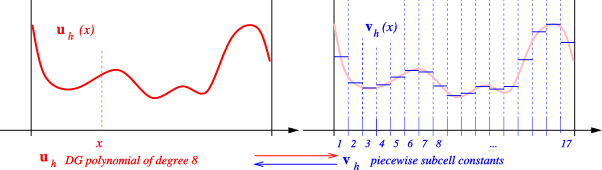
\includegraphics[width=\textwidth]{limiting-grid/limiter-P7bis-single.pdf}
	\caption[
	  Sketch of the DG-FV limiting projection/restriction,
	  \modifiedAfter{Dumbser2014,exahype-guidebook}
	]{
		A cartoon which demonstrates how a high order 
		Discontinous Galerkin solution/polynomial $u_h$ within a single patch
		(red)
		is projected onto $2N+1$ finite volume subcell averages (blue).
		The projection works in both ways, whereas the one from the higher
		amount of degrees of freedom (FV limiter) is called \emph{restriction}.
		Figure modified from
		\cite{Dumbser2014,exahype-guidebook}.
	}\label{fig:aderdg-limiter-2np1}
	% Is the citation correct? It was Dumbser2014b before.
\end{figure}
	
 In practice, each
 computational cell $\Omega_i$ that has been marked for limiting is split
 into $(2N+1)^3$ finite-volume subcells, which are denoted by
 $\Omega_{i,s}$ and that satisfy $\Omega_i = \bigcup_s \Omega_{i,s}$ (see
 Fig. \ref{fig:aderdg-limiter-2np1}). Note that this very fine division of a DG
 element into finite-volume subcells does \textit{not} reduce the timestep
 of the overall ADER-DG scheme, since the Courant-Friedrichs-Lewy (CFL)
 coefficient of explicit DG schemes scales with $1/(2N+1)$, while the CFL
 of finite-volume schemes (used on the subgrid) is of the order of
 unity \cite{Dumbser2014,Zanotti2015c,Zanotti2015c,Zanotti2015d,ADERDGVisc}.
 The discrete solution in the subcells $\Omega_{i,s}$ is
 represented at time $t^n$ in terms of \textit{piecewise constant} subcell
 averages $\bar{\u}^n_{i,s}$, \ie \footnote{as in Godunov's scheme,
 	eq. \eqref{eqn.subcellaverage} }
 %
 \begin{equation}
 \bar{\u}^n_{i,s} := \frac{1}{|\Omega_{i,s}|} \int \limits_{\Omega_{i,s}}
 \Q(\x,t^n) d \x\,.
 \end{equation}
 %
 These subcell averages are evolved in time with any {suitable}
 finite-volume scheme. \footnote{See Section~\ref{sec:fv} for a presentation of
   finite volume schemes. The \code{ExaHyPE} paradigm to decide
   \emph{suitability} is to assume that robust finite volume methods for
   a given problem are understood and can be used as a safe \emph{fallback}
   in case of problematic DG solutions which require limiting.
 } 
 
 In fact, the limiting ADER-DG (or: hybrid) scheme can be understood as
 a DG solver  coupled to a FV solver, acting on the same grid. To do so,
 on a limited patch, the ``embedded'' DG quadrature points are replaced by
 an equally embedded finite volume grid. The resulting limited 
 finite volume patch has a block-regular structure of $(2N+1)$
 cells (see Section~\ref{sec:block-regular-grids} about block regular grids). 
 
 From the finite volume scheme, a new piecewise constant solution $\boldsymbol{v}_h(\x,
 t^{n+1})$ given by the cell averages $\bar{\boldsymbol{v}}_{i,s}^{n+1}$
 is obtained, from which the final, {limited} DG
 polynomial as $\boldsymbol{u}_h(\x,t^{n+1}) = \mathcal{R}\left( \boldsymbol{v}_h(\x,t^n) \right)
 $ is reconstructed, where $\mathcal{R}$ is the reconstruction operator associated with the
 projector $\mathcal{P}$, so that $\mathcal{R} \circ \mathcal{P} =
 \mathcal{I}$, with $\mathcal{I}$ the identity operator \cite{Dumbser2014}.
 %
 For the subcell finite-volume scheme a different CFL stability condition
 applies and takes the form
 \begin{align}
 \Delta t_{\text{FV}} < \text{CFL}\frac{h_{\text{min}}}{d \, N_s}
 \frac{1}{|\lambda_{\text{max}}|}, \label{eq:CFLweno}
 \end{align}
 with $h_{\min}$ the minimum cell size referred to the DG control volumes
 $\Omega_i$ and $\lambda_\text{max}=|\Lambda_i|$ the maximal wave speed of the
 system. Choosing $N_s \geq N+1$ is a natural requirement that allows
 to reconstruct the of degrees of freedom of $\boldsymbol{u}_h$ from the piecewise
 constant solution $\boldsymbol{v}_h$ via $\mathcal{R}$. Following \cite{Dumbser2014}
 we choose $N_s = 2N + 1$ so that $\Delta t_{\text{FV}} = \Delta
 t_{\text{DG}}$. This choice allows us to maximise the resolution
 properties of the chosen subcell finite-volume scheme and to run it at
 its maximum possible CFL number. 


When considering time integration, in ADER schemes for nonlinear hyperbolic PDE,
limiters need to be applied only once per time step, while in Runge-Kutta based 
MoL schemes, the limiter needs to be applied in each Runge-Kutta 
stage again \footnote{
    For a detailed comparison of Runge-Kutta and ADER
	finite-volume schemes, see \cite{dumbser_diffapprox} and
	\cite{Balsara2013}, while Runge-Kutta DG and Lax-Wendroff DG schemes
	(the latter are very similar to ADER-DG schemes) have been compared in
	\cite{QiuDumbserShu}, also concerning computational performance. Detailed
	computational performance comparison between ADER-DG schemes and RKDG
	schemes are also given in Appendix~\vref{sec:rkdg-performance}.}.

%=============================================================
%\newpage % for simplicty with the figures here
\section{Grid meshing}\label{sec:grid-meshing}
The issue of storing the data necessary for the presented numerical schemes is
tightly coupled to the representation of the numerical grid on the computer. This is
a technical challenge continously addressed by computer scientists, since computer
architectures are evolving in time and different aspects get important.

In this section, a couple of aspects are presented in a generic fashion, \ie there
is no particular focus on FD, FV or DG methods and it is left open what the grid
actually holds (point/vertex data, cell averages or cells with a subcell structure).

\subsection{Block regular grids}\label{sec:block-regular-grids}
\begin{marginfigure}
	\includegraphics[width=\linewidth]{numerics-grids/cactus-components.png}
	\caption[
	  Sketch of Carpet grid covering, \modifiedAfter{carpet_web}]%
	{A height-elevated plot of a scalar field on a two-dimensional domain. The displayed
	 grid structure reveals a unigrid layout. Multiple patches are shown which cover the
	 physical domain, each having the same resolution $\Delta \vec x$. Color is used
	 to distinguish the patches. Furthermore, the overlapping ghost zones are displayed
	 in a different colour. Figure modified from~\cite{carpet_web}.}%
	\label{fig:numerics-cactus-components}
\end{marginfigure}
%
The simplest grids are \emph{regular} (or \emph{uniform}, also refered to as \emph{unigrid}),
that means each grid coordinate
\begin{equation}
\vec x = \sum_{i=0}^d x_i \Delta x^i
\end{equation}
can be described by the constant vector of grid spacings $\Delta \vec x \in \mathbb{R}^d$ and
integer position indices $\vec x \in \mathbb{N}^d$. Therefore, a finite domain grid is fully
characterized
by the grid spacings $\Delta \vec x$ and a description of the domain, for instance
$\vec x = \vec x_0 + x_i \Delta x^i$ with offset $x_0$ and $x_i \in [0,N]^d$ with $N$
being the number of points.

Uniform grids can be Cartesian (unit squares, $\Delta x^i=\Delta x~\forall i\in[1,d]$)
or rectilinear (all $\Delta x^i$ may be different from each other). They also may be
curvilinear, for instance in a cylindrical or spherical coordinates mapping.
In contrast, irregular grids are called \emph{unstructured} and a priori a list of all
grid points must be stored.

Figure \ref{fig:numerics-cactus-components} shows the grid structure in an exemplaric setup
how it is used by the \code{Carpet} code, which is part of the \code{EinsteinToolkit}
\footnote{See appendix \vref{apx.codes} for details about the codes referenced in the main text.}.
Carpet implements block regular grids, \ie each of the displayed three blocks is a regular grid.
In practice, different blocks are evolved in time by different processors/computers.
For the implementation of the particular FD/FV scheme, exchange of information at the boundaries
of each block is neccessary, which is faciliated by a small overlap of the patches. Cells within
the overlapping region are called \emph{ghost cells}. Figure \ref{fig:numerics-cactus-components}
shows one layer of ghost cells around each block.

%Implementing block regular grids is an old technique and was already done 50 
%years ago.

\subsection{Mesh refinement}\label{sec:mesh-refinement}
\begin{marginfigure}
	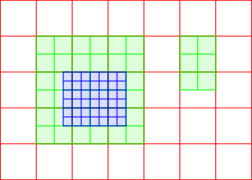
\includegraphics[width=\linewidth]{numerics-grids/Carpet-FMR.pdf}
	\caption[Carpet FMR region sketch, \colorizedAfter{Schnetter-etal-03b}]%
	{Multiple Fixed Mesh Refinement layers (FMR) in Carpet, from \cite{Schnetter-etal-03b}}%
	\label{fig:numerics-cactus-fmr}
\end{marginfigure}
%
\begin{marginfigure}
	\includegraphics[width=\textwidth]{numerics-grids/quadtree.png}
	\caption[
	AMR vs unigrid in 2D, cartoon, \modifiedAfter{Sortino2009quadtree}]%
	{   Resolving a curve in a unigrid ($16\cdot 24=384$ elements) vs.
		a local mesh refinement (quadtree, $6+12+48+96=166$ elements)
		with the same resolution, but only 43\% storage.
		Adopted from \cite{Sortino2009quadtree}.}\label{fig:amr-motivation}
\end{marginfigure}
%
Grid codes implement mesh refinement in order to resolve local features while being able to
evolve a large spatial domain. As refinement layers are supposed to have smaller cells, they also
have smaller maximum timestep sizes (due to the CFL condition). A code with \emph{global time
stepping} evolves all refinement levels with the maximum timestep size of the finest layer,
this typically leads to numerical dissipation in the coarser layers and is very slow, as
the coarser layers allow bigger timesteps. Therefore, a proper refinement code implements
\emph{local time stepping} where each refinement level is evolved with the maximum time step
possible locally. Depending on the scheme and implementation, this requires prolongation 
(projection of field values from the finer to the coarser levels) and restriction
(projection of field values from the coarser to the finer levels)
in order to make use of the finer resolved data at the different time levels.

The \code{Carpet} code implements \emph{Fixed} Mesh Refinement (FMR),
also refered to as \emph{moving boxes} or \emph{boxes in boxes}. The concept is visualized
in Figure \ref{fig:numerics-cactus-fmr} where three refinement levels are displayed (here
without ghost zones). Refinement layers can be ordered by their resolution, this motivates
to collect them in tree-structures \cite{Khokhlov98}.
Typically, codes restrict to a single refinement factor $k$.
Given a numerical scheme with convergence order $\alpha$, the convergence (refinement)
factor of the overall code will be $k\alpha$.

The dynamical version of FMR is Adaptive Mesh Refinement (AMR), where the refined areas are
created, moved and destroyed by a criterion such as a treshold on a degree of freedom
(Figure~\ref{fig:amr-motivation}).

Dynamical load-balancing (of a dynamical AMR grid) is an open research problem in
computer science. A difficulty is to detect load inequalities, moving load between nodes
and assessing the effectiveness of such an expensive operation. A code with \emph{static}
load balancing (of a static AMR problem) can circumvent this in advance by hand-crafted
distribution of work.

\begin{marginfigure}
	\includegraphics[width=\textwidth]{grmhd-paper-official/AMR_levels.pdf}
	\caption[Space-Tree illustration, TikZ figure \by{Fambri},
	  \publishedIn{Fambri2017}]{The
		\emph{space-tree} structure of the refinement levels for a single
		element at the coarsest level $\ell_0$ is shown, corresponding to the
		choice $\mathcal{R}=3$. Figure published in \cite{Fambri2017}. }
	\label{fig:numerics-AMR-single-cell}
\end{marginfigure}
%
Further aspects of mesh refinement are the starting paradigm: For instance,
being a sane Octree code, the \code{ExaHyPE} code refines from a \emph{single cell},
that is, it is an AMR code by heart (Figure \ref{fig:numerics-AMR-single-cell}).
In contrast, the \code{ExaHyPE} prototype codes as well as \code{Cactus} start with 
an already refined unigrid. At startup,
this allows for Cartesian slicing which minimizes the surface of the
blocks right at the beginning but postpones the load balancing problem to later
refinement steps.

\subsection{Parallelization}
\begin{marginfigure}
	\includegraphics[width=\linewidth]{peano-task-graphs/tasks.pdf}
	\caption[
	  Idealized ExaHyPE/Peano task graph. Modiefied from \cite{exahype-review}.
	]{
		Idealized parallel task graph in \code{ExaHyPE}.
		Modified from \cite{exahype-review}.
	}\label{fig:exahype-task-graph}
\end{marginfigure}
Hyperbolic laws with finite wave speeds invite to parallelize on the spatial
domain. Modern codes need to exploit parallelism on several hierarchies. On the
programming level, the HPC landscape is dominated by shared and distributed memory
parallelization (MIMD, multiple instruction, multiple data) as well as vectorization
(SIMD, single instruction, multiple data).
%The approach taken here distinguishes all codes mentioned so far from each other most.

The \code{Cactus} framework manages the distributed memory parallelization internally by
splitting up the simulation domain. The split follows a traditional Cartesian
domain composition. In \code{Cactus}, program modules (\emph{thorns}) 
allow for random read
and write access to the grid, have to describe the numerical schemes and the physics
(PDEs). They need to implement shared memory parallelization as well as
vectorization.
In contrast, the \code{ExaHyPE} framework manages both distributed and shared memory
parallelization, so that users are only confronted with providing their PDE in a
vectorizable way \footnote{
 Section \ref{sec:fo-ccz4-implementations} provides a discussion of
 vectorized implementations of the CCZ4 formulation of Einsteins Equations.}.
Being an active research code for AMR, \code{ExaHyPE} implements a number
of state-of-the-art domain
decomposition paradigms, for instance it dimensionally reduces the computational domain
by \emph{domain filling curves}, thus mapping physical locality to memory locality.
This is useful for hyperbolic conservation laws where causality implies that significantly
seperated spatial regions do not influence each other.
The mesh code in \code{ExaHyPE} is called \code{Peano} (like the spacefilling curve)
and uses two coupled state machines (finite automata) 
to couple a numerical scheme to the grid traversal
(Figure \ref{fig:peano-finite-automata}). This formalization
allows to optimize the code in numberous ways (such as doing research on task
based graphs, Figure \ref{fig:exahype-task-graph})
but locks down the
scheme to the predefined actions, prehibiting random access and
attemps done in classical codes \cite{Weinzierl2015}. This paradigm is called
``principle of loosing control'' (or ``Hollywood principle'', ``inversion of
control'') and is typical for application frameworks.

\begin{marginfigure}[-2cm]
\makebox[\linewidth][c]{% centering figure
	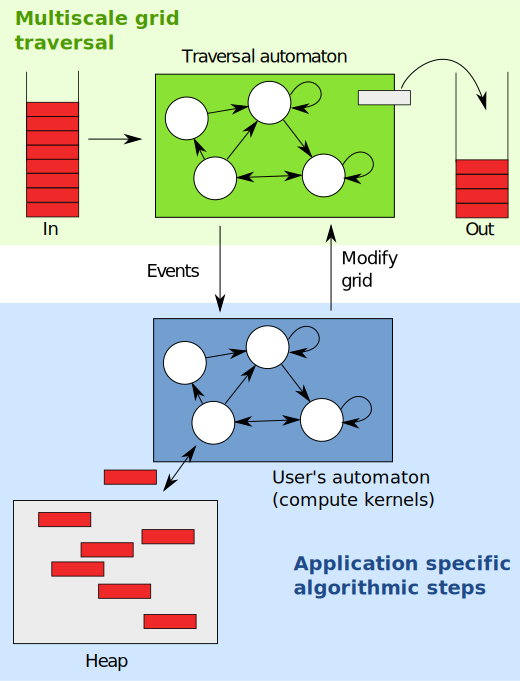
\includegraphics[width=1.05\linewidth]{peano/automata-less-width.pdf}
}% end makebox
	\caption[
  	  Finite state machines of Peano, \modifiedAfter{Weinzierl2015} 
  	%arXiV:1506.04496
	]{Cartoon of the \code{Peano}/\code{ExaHyPE} architecture.
	  Figure modified from~\cite{Weinzierl2015}.}
	\label{fig:peano-finite-automata}
\end{marginfigure}

\subsection[ADER-DG $hp$-refinement]{$hp$-refinement with ADER-DG and subcell 
limiter}
The ADER-DG algorithms with subcell finite-volume limiter described above
has been here implemented on spacetime adaptive Cartesian meshes. Details
on the used AMR algorithm are described in
\cite{AMR3DCL,Zanotti2015c,Zanotti2015c,Zanotti2015d,ADERDGVisc}.
The AMR strategy adopted is named
\emph{cell-by-cell} refinement and consists in providing a space-tree data
structure \cite{Khokhlov98, Peano1, Peano2, AMR3DCL},
whose \emph{leaves} correspond to the spatial elements $\Omega_i$ used by
the numerical scheme described before. The main alternative to a
space-tree data structure is the use of  \emph{patches},
\cite{Berger-Oliger1984, berger85, Berger-Colella1989}, where a
set of independent overlaying Cartesian sub-grid domains (or patches)
is introduced and activated when necessary. In the AMR approach used in
\code{ExaHyPE}, the numerical solution is checked independently along every single
space-element for an eventual recursive refining or recoarsening
process.
%
In practice, starting from an initial Cartesian grid of refinement level
$\ell=\ell_0=0$, which is the basic mesh without refinement, the
tree-type infrastructure of finer {refinement levels} is made
accessible. The refinement levels $\ell>0$ are built according to the so
called {refinement factor} $\mathcal{R}$, which is the number of smaller
space-elements per space-direction in which a coarser element is broken
in a refinement process, or which are merged in a recoarsening
stage. Note that choosing a refinement factor $\mathcal{R}=2$ would
generate the well known \emph{quadtrees} in two-dimensional (2D) meshes and
\emph{octree} in 3D meshes. For an arbitrary refinement factor
$\mathcal{R}$, general space-trees are obtained \cite{Peano1,Peano2}.

\begin{marginfigure}
  \includegraphics[width=\textwidth]{grmhd-paper-official/AMR_DGSubcell.pdf}
  \caption[
     AMR and DG cartoon, drawn \by{Fambri}, \publishedIn{Fambri2017}
    ]{An example of combination of AMR and DG subcell
    reconstruction is shown. The limited cells ($\beta=1$)
    $\mathcal{C}_n$ and $\mathcal{C}_m$ are highlighted in red. The
    simplest way for the polynomial reconstruction between
    $\mathcal{C}_n$ and $\mathcal{C}_m$ elements is: (i) project the
    piecewise constant solution from $\mathcal{C}_n$ to the virtual
    child-element $\mathcal{C}_v$ (see Fig.~\protect\ref{fig:AMRmaps}); (ii) do
    polynomial reconstruction along the same refinement level, between
    $\mathcal{C}_v$ and $\mathcal{C}_m$.
    Figure published in \cite{Fambri2017}.
    }
  \label{fig:AMR}
\end{marginfigure}

For practical purposes, a finite number of refinement levels is provided,
\ie from the coarser $\ell = \ell_0$ to a finest possible refinement
level $\ell = \ell_{\text{max}}\in{\rm I\!N}^+_0$. The
refinement/recoarsening process is driven by the standard \emph{Loehner scheme}
\cite{Loehner1987}, \ie a prescribed {re\-fine\-ment-estimator function}
\begin{equation}
\chi(\varphi) =
\sqrt{	\frac{
		\sum_{k,l} \left( \partial_l \partial_k \varphi \right)^2
		}{
		\sum_{k,l} 
		  \left(
          \frac{
			\left| \partial_k \varphi \right|_{i+1} + \left| \partial_k \varphi \right|_i
		  }{\Delta x_i}
		  + \epsilon
		  \left| \partial_k \partial_l \left| \varphi \right| \right|
		  \right)^2
		}
}
\end{equation}
which is a function of discrete gradients and second derivatives of a scalar
\emph{indicator function}
${\varphi}= \varphi\left(\boldsymbol{u}_h(\x,t^n)\right)$
and by two thresholds $\chi^+$ and $\chi^-$
\cite{Loehner1987,Zanotti2015d,ADERDGVisc}. Elements are
marked for refinement whenever $\chi > \chi^+$ and for recoarsening
whenever $\chi < \chi^-$. Examples for the indicator function $\varphi$
in hydrodynamics are the rest mass density ($\varphi=\rho$), production
of entropy \cite{PS:entropy, SCR:CWENOquadtree, CS:epsweno}, the Lorentz
factor, as well as geometric criteria ($\varphi=\varphi(\vec x)$).

To simplify the AMR algorithm, two neighbour elements are allowed to
belong either to the same level $\ell$ or to an adjacent refinement level
$\ell \pm 1$. To each element in the tree we assign a basic {element
  status} which is
%
\begin{align}
\sigma_i &= \left\{\begin{array}{rcl} 
-1\,, & & \text{for the  \emph{parent cells}} \\
\phantom{-}0\,, & & \text{for \emph{active elements}} \\
+1\,, & & \text{for the  \emph{virtual children}}
\end{array}\right. \nonumber \\
 i&=1,\ldots, N_{\text{tot}},
\end{align}
%
where $N_{\text{tot}}$ is the total number of space-elements present in
the tree. Note that $N_{\text{tot}}$ should be distinguished from the
total number of {active} elements $N_E$, which are the leaves of the tree
that define the $\Omega_i$ used in the numerical scheme, and for which
$N_{\text{tot}}>N_E$ holds in general. The  {parent cells}
($\sigma_i=-1$) are those tree elements which contain active elements on
a higher level and finally a {virtual child cell} ($\sigma_i=+1$) is a
tree element which is {contained} within an active cell that belongs to a
{lower} and {adjacent} refinement level $\ell-1$.

\begin{figure}[t]
\includegraphics[width=\textwidth]{grmhd-paper-tikz/standalone-AMR_maps.pdf}
\caption[
   Restriction and projection with AMR, drawin \by{Fambri},
   \publishedIn{Fambri2017}
 ]{Mapping of the numerical solution between the piecewise
  polynomials $\boldsymbol{u}_h$ of the DG scheme and the piecewise constant data
  $\boldsymbol{v}_h$ of the finite-volume scheme as well as between two different
  AMR-levels $\ell$ and $\ell+1$. Figure published in \cite{Fambri2017}.}
\label{fig:AMRmaps}
\end{figure}

Apart from the storage of flux contributions from neighbour cells within
our high-order time-accurate local time stepping (LTS) algorithm
\cite{AMR3DCL}, virtual cells are also needed for high-order
finite-volume schemes to provide the necessary data for polynomial
reconstructions (TVD, WENO) on a given refinement level if two adjacent
active cells belong to {different} refinement levels; this is illustrated
schematically in Fig. \ref{fig:AMR}. This strategy produces a locally
uniform grid around each cell and greatly simplifies reconstruction. Our
strategy of generating a locally uniform grid around each cell is very
different from the approach based on genuinely multidimensional CWENO
reconstructions proposed by \cite{SCR:CWENOquadtree}.

The dynamics of the numerical solution on virtual elements is given by
standard $L_2$ projection (for virtual children) or averaging (for parent
cells), as depicted in Fig. \ref{fig:AMRmaps}, where the mapping between
the chosen solution spaces, piecewise polynomial (unlimited) or
piecewise constant (limited), and between two adjacent refinement levels
$\ell$ and $\ell+1$ is depicted.

Due to the possibility of handling a large range of spatial
scales within the same domain, corresponding to very different CFL time
restrictions, a time-accurate and fully conservative {local time
  stepping} (LTS) has been implemented in order to use the smallest
admitted timestep only where necessary, and a large timestep where it is
allowed \cite{AMR3DCL}.

Within the \code{ExaHyPE} code, the adaptive mesh refinement can further
be triggered by the finite volume subcell limiter, which is always applied
at the finest AMR level of the simulation. In such a case, a padding is
applied around the limited regions
\cite{exahype-review,exahype-guidebook}.

%


\section[
  Aspects of input and output on AMR and DG
]{Aspects of input and output on adaptive meshes and discontinous
  Galerkin methods}
For completeness, this section presents a few aspects of input and output in
a numerical time evolution code, especially in the context of dynamical AMR
and DG. These features were implemented for the \code{ExaHyPE} code.

\subsection{In-situ initial data}
Reading initial data on an AMR grid is more challenging then on a predefined
grid, as local features in the initial data shall already be resolved, not only
features which appear after certain time during the evolution. In order to
setup an AMR grid hierarchy which adaptively adopts to non-analytical initial
data, an AMR grid code needs to evaluate the refinement criterion on the ID.

One way to do this is to evaluate the initial state $Q_0(\vec x)$ on subsequent
grid levels until the required accuracy is gained. At the same time, in the
context of parallelism, an AMR code has to load balance the spawned spacetree
over the available processors.

% SOURCE: 
%http://sven.köppel.org/uni/ws1617/2017-04-03-ExaHyPE-ReviewMeeting-FIAS-SK/
% Another source: ExaHyPE guidebook
\begin{marginfigure}
	\includegraphics[width=\textwidth]{dg-fv-id-derivatives/01_initial.pdf}
	\includegraphics[width=\textwidth]{dg-fv-id-derivatives/02_projection.pdf}
	\includegraphics[width=\textwidth]{dg-fv-id-derivatives/03_derivative.pdf}
	\includegraphics[width=\textwidth]{dg-fv-id-derivatives/04_fd_local_derivs.pdf}
	\caption[
	FV vs DG derivatives for ID, drawn with Inkscape, \exclusive
	]{Cartoon of FD vs. DG derivatives for initial data in one dimension.
		Each panel shows the same exemplaric patch, where a fifth order DG polynomial
		is embedded on a Euler-Legendre nodal basis (\ie the filled circles indicate the
		spatial positions where the field values are stored).
		First panel: The exemplaric field solution which is subsequently projected
		onto the DG polynomial (green, second panel) and subsequently differentiated
		(blue, third panel). In contrast, the last panel shows the cartoon of a
		finite differencing stencil for off-grid computation of the initial data
		around a requested point. Here, the initial data have to be provided at
		each bullet, \ie have to be provided five time as much as in the DG derivative
		case.
	}
	\label{fig:dg-fv-id-derivatives}
\end{marginfigure}

The paradigm shift from a classical block-regular code (such as \code{Carpet}) towards
an AMR code (such as \code{ExaHyPE}) shall be demonstrated on an example: As per
definition, a-priori there is no grid, the evaluation of an initial data
(ID)
subroutine has to happen locally for a given spatial point $\vec x$. Typically,
within this thesis, initial data itself are the numerical solution of an
elliptic PDE and therefore present on a certain grid. Reading in the data from
the ID code to the time evolution code typically results in interpolating
between two grids.

As soon as non-local computations are neccessary, this attemp fails. An example
are initial data available as solution of a second order elliptic PDE but
to be evolved with a first order formulation of that PDE (as with the 
formulation of Einstein field equations presented in 
section~\ref{sec:fo-ccz4}). In this case,
auxilliary fields $a_i = \partial_i \phi$ for some field $\phi$ have to be
computed, and the derivative operator is nonlocal by definition.

The two solutions are either to precompute the auxiliary field also on the
initial data code grid, or to compute them on-demand (in-situ). The later
option is preferable to have point-wise access to the initial data in the
time evolution at any time. For computing derivatives, in \code{ExaHyPE} we chose
two approaches (Figure~\ref{fig:dg-fv-id-derivatives}): Patchwise, using
the DG derivatives (which can be thought of a semi-local attempt) or off-grid with finite
differences.

\subsection{In-situ postprocessing}
Within the time evolution codes presented so far, it is common practice to
write out the system state also during the time evolution (and not only at
its arbitrary end). This outputting is done repeatedly by a time or iteration
criterion (formulated for instance as ``write every $N$th iteration'' or 
``write every $\Delta t$''), but any other kind of \emph{query based plotting}
can be imagined. \footnote{We use the terms \emph{plotting}, \emph{writing},
	\emph{dumping} of data synonymously.
} The concept of a writeout is to store 
the current \emph{snapshot}
$\u(t,\x)$ for a given time $t$ permanently, while it is neccessarily erased
at one point in an evolution scheme which thrives to have a constant memory
need during time evolution.

When it comes to the writeout phase, any kind of \emph{postprocessing} can be
done. This term shall be defined by a local mapping
$f: \mathrm \Omega^n \to \mathrm \Omega^m$ which maps the solution vector
$\u(\x)$ at a fixed given time $t$
to a vector of written quantities $\boldsymbol w(\x)$ on the spatial 
$d$-dimensional simulation domain $\Omega$\footnote{
  This mapping can be non-locally extended to allow for derivatives, such
  as $\boldsymbol w(\x) = f(\u(\x), \partial_i \u(\x), \dots)$.
}. One can imagine that
$\boldsymbol w = \boldsymbol f(\u)$ is computed either during the time
evolution (``online''), in order to write out \emph{only} the mapped state
vector, or afterwards, so $\u$ is written and $\boldsymbol f(\u)$ is computed
in an offline postprocessing step. 
Online post processing might save a lot of computing ressources
if $m \ll n$ and $\boldsymbol f$ is computationally cheap.

Reductions or volume/surface integrals can be modeled with a mapping
$g: \mathrm R^{d\times n} \to \mathrm R^{e \times m}$, where $e<d$ is the
dimensional reduction and again $m<n$ stands for a lossy mapping of the
solution vector to less degrees of freedom. For the highly symmetric spacetimes
of compact objects, as presented in the next chapters, simple 1D and 2D cuts
of the Cartesian coordinate systems on the axis are typical dimensional
reductions, while $L_1$, $L_2$ and $L_\infty$  (volume) integrals are evaluated
on the whole space and provide ``0D'' scalar output. Surface integrals over
an arbitrary surface (defined by its normal vector field $S^i$) are technically
more complex to implement but nevertheless fall into the class of mappings $g$.
\todo[color=green]{
  In-Situ postprocessing: Could give examples, such as
  ADM Mass, Angular momentum, Apparent Horizon
  detectors. Something different are tracers/trackers (nonlocal)
}

\subsection{Visualization of ADER-DG simulations}
When simulation data should be stored permanently, a well-defined file format
provides interoperability between different (possibly postprocessing) codes.
The \code{ExaHyPE} grid structure can be casted as \emph{block regular}:
The DG polynomials in each patch can be sampled on a unigrid, without loss
of accuracy (\ie by keeping the number of nodal points the same). This is
the basic idea of the implementation of the \code{CarpetHDF5} file format
within \code{ExaHyPE},
which was originally developed for \code{Carpet} \cite{Reisswig:2010}.

While the \code{CarpetHDF5} \footnote{
  \code{HDF} is short for ``Hierarchical Data Format'' and is a container file format
  for scientific data, especially multidimensional arrays. In principle,
  the propsed discussion is independent of the container file format.
  See \cite{exahype-guidebook} for details about the file formats.
  
  In contrast to the formats discussed in the main text,
  \code{VTK} (``Visualization Toolkit'') is a widely supported
  standarized format for describing higher dimensional geometries.
  \code{ExaHyPE} can write \code{VTK} files, but these files are only
  optimized for interoperability.
} file format is tailored to the memory layout of
\code{Carpet}, where block regular \emph{components} are sized in order to
match one parallel rank (\ie a MPI process), in \code{ExaHyPE} the patches
are kept intentionally small to hold a single DG polynomial. Therefore,
the number of patches per dimension is typically one to two orders of
magnitude larger in \code{Carpet} grids compared to \code{ExaHyPE} grids,
and the amount of \emph{meta data} in the \code{CarpetHDF5} file format
dominates over the \emph{payload data}. In this context, the term ``meta
data'' refers to the description of the grid structure and component
geometry, while ``payload data'' are the actual field values. This
property makes the \code{CarpetHDF5} format especially inattractive
in \code{ExaHyPE} as a volumetric file format
(\ie in three spatial dimensions). \footnote{
  The structure-of-array/array-of-structure representation of fields
  is the underlying difference between \code{Carpet} (basically
  storing $(Q_0(\vec x), Q_1(\vec x), \dots)$ and \code{ExaHyPE}
  (storing $\vec Q(\vec x_0), \vec Q(\vec x_1), \dots)$).
  This is also the main difference between the Carpet file format and
  the tailored Peano block regular file format~\cite{exahype-guidebook}.
}


\section{Summary}
In Chapter~\ref{chapter:numerics}, all the ingredients for a new code developed
within this thesis were proposed. At the very heart, it is a coupled
evolution scheme which uses a local ADER-DG scheme which is by construction
communication avoiding and thus suitable for the next generation of
machines, in contrast to traditional schemes, as well as an undemanding
traditional Finite Volume scheme, which is however time variation diminishing
and suitable to evolve a solution at low order. The infrastructure
for running three-dimensional astrophysical simulations was presented, and it
will be brought to life in the subsequent chapters \vref{chapter:gr}
(with general relativity) and chapter \vref{chapter:hydro}
(with hydrodynamics).








\subtitledChapter
   {A first-order formulation of the Einstein equations and its solution with DG schemes}
   {General Relativity}\label{chapter:gr}
This chapter summarizes the efforts of writing Einstein Field equations
(EFE) \cite{Einstein15a,Einstein15b} in a way specially suitable for
high (convergence) order numerical integration, with the numerical
schemes presented in chapter~\ref{chapter:numerics}. For an introduction
into the problem and a review of previous work, see
Section~\vref{sec:gr-intro-intro}.
This chapter relies partially on the coauthored publications
 \cite{Dumbser2017} as well as \cite{Koeppel2017}.

\section{Motivation: The two body problem of GR}\label{sec:gr-intro}
Exact solutions of Einstein Field equations are ``rare'' \cite{Kramer80}
and well known solutions are highly symmetric spacetimes. Two astrophysically
relevant examples are the stationary Kerr black hole (two Killing vectors:
rotational / azimuthal and in time direction) and the static TOV solution of an
isotropic fluid in equilibrium (spherically symmetric, thus three orthogonal
spacelike Killing vectors)\footnote{
    The TOV solution is refered here synonmyously to as TOV star or neutron star.
    
	Particular spacetimes are introduced in the benchmark 
	sections,
	for instance the Kerr(-Schild) solution in 
	Section~\vref{sec:convergence-bh3d} and the TOV solution 
	in Section~\vref{sec:tov}. 
}.

\begin{marginfigure}
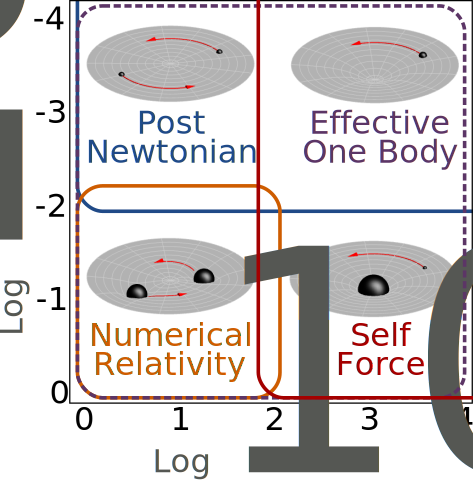
\includegraphics[width=\textwidth]{efe-intro-2body/2BodyEFE-SvenDrawing.pdf}
\caption[
  EFE 2body parameter space, drawn with Inkscape. \exclusive
]{
 Practicability/availability diagram of the two body problem in GR with
 the parameter range archieveable with approximations.
}
\label{fig:efe-intro-2body-paramspace}
\end{marginfigure}
%
Being a nonlinear theory where the superposition principle no longer holds (in contrast
to classical and quantum mechanics), the two body problem 
%for these two exemplaric objects
in (full) general relativity (GR) is nontrivial. That is, there is no way of analytically solving Einstein field
equations exactly for a spacetime holding two compact objects (black holes or neutron stars).
Instead, all attemps to find such spacetimes are using approximations which however
can be subsequently refined to converge to the real solution. The two major approximation
scales are
%\\
(1) the mass ratio $M_1/M_2$ of the two objects and
%\\
(2) the compactness $C=M/R$ of the system, with $R$ the object
seperation and $M=M_1+M_2$ the total spacetime mass
\cite{MTW1973,Wald84,Buonanno2014}. Due to the virial theorem, this
scale is similar to $v^2/c^2$ with the characteristic velocity $v$ of an object in the
binary system.

It is popular to inspect the two-dimensional space spanned by these two parameters
in a diagram (Figure \ref{fig:efe-intro-2body-paramspace}): Two perturbation theories
cover either the small compactness or the high mass ratio regime. The first one is
the Post Newtonian (PN) expansion of EFE where the velocity ratio is small compared to the speed
of light. The second one are gravitational self-force corrections \cite{Wald:2009ue} which
correct around an infinite mass ratio (static approximation of the heavier object /
test particle on a geodesic in an external metric).
Being analytic theories which approximate Einstein equations, for a given order of
approximation, these theories fail to describe a binary system with high mass, finite extend,
rapid rotation. In order to describe this strong gravity regime correctly, Einstein equations
must be solved without simplifying approximations. The answer from numerical relativity (NR) is to
approximate the spacetime itself instead of the field equations. The mathematical approach is
no more analytic but numerical, working on discretized fields, whereas the ``full'' Lagrangian
is solved, without the (computational/mathematical) need for a simplification.
\footnote{
It is interesting to do an excursion to the other popular nonlinear theory
in high energy physics, since there are similar approximations done: Quantum chromodynamics
(QCD), the special relativistic quantum theory of the strong force,
 part of the Standard Model of elementary particles and suitable for 
 describing, for instance,
 fundamental baryonic and mesonic particles hold together by the strong force.
The two body problem in QCD in the context of heavy quarks has a similiar parameter
space with similiar solutions: Instead of Post Newtonian
expansion, there is non-relativistic QCD, while the heavy quark effective theory is
renowed for describing dynamic quarks in the presence of infinetely heavy quarks. However,
in the relativistic regime of two quarks with similar mass, the full QCD Lagrangian must be
solved to predict correct observables. A successful theory to do so discretizes spacetime
(with periodic boundary conditions, therefore referred to as a ``lattice'') where
a QCD Lagrangian (not neccessarily describing all flavours) is solved
numerically. This research field is called Lattice QCD. At the present, numerical relativity and
lattice QCD are the two major challenging applications in high energy computational physics.
} % footnote
In practice, however, it is a long way to recast the Einstein field equations in a hyperbolic
way, suitable for ``time'' integration, and the following Sections will provide an
insight into the approach used within this work.

This broad-brush motivation for numerical approaches in field theory disregards
many successful attemps of covering the whole parameter space of Figure \ref{fig:efe-intro-2body-paramspace}
analytically. In case of GR, there is the effective one body formalism which is able of
an analytic treatment of the strong gravity regime of two body spacetimes by taking into
accounts results from PN and NR~\cite{Damour:2008yg,Buonanno:1998gg}. In contrast, numerical
relativity is the only approach to arbitrary strong gravity spacetimes which works from
first principles, \ie without any external input, and that can in principle cover the whole
space.

\section{The Cauchy Initial value formulation of GR}%
\label{sec:adm}%
%
General relativity is invariant under the Lorentz (Lie) group, that makes it a gauge
theory. The four degrees of freedom (DOF) from Lorentz group can be cast in 
general smooth coordinate transformations $x'_\mu = f_\mu(x)$ and this 
invariance is known as general or diffeomorphism covariance. From the
$4\times4=16$ components of Einstein equations, only 10 are independent, and
the gauge freedom removes another 4~DOF, thus 6 
physical DOF remain.

The ADM formulation (dating back to 1959 by Arnowitt, Deser, Misner
\cite{Arnowitt62}) is an Hamiltonian formulation of Einstein
field equations.
\footnote{
  We will refer to the ADM formulation synonymously to as the (Cauchy)
  initial value problem	formulation or the canonical formulation of EFE.
} It allows to define a time coordinate and thus to perform
a time evolution on the orthogonal spatial coordinates 
(\cf Section~\ref{sec:hamiltonian-motivation} on
Hamiltonian time evolution).
The ADM formulation is one way to identify/fix the gauge degrees of gravity
by dimensional reduction and restricting Einstein field equations on the
lower-dimensional hyperspaces (\eg $D=4$-dimensional spacetime is restricted on
3-dimensional hypersurfaces)\footnote{
	The ADM split, or rather the ADM canonical coordinates, are not a unique choice.
	The Ashtekar variables \cite{Ashtekar1986}, which rewrite three-dimensional slices into
	SU(2) gauge fields, are an example of a popular differen choice which is actually
	the foundation of loop quantum gravity \cite{Rovelli2008}.
}. Arbitrarily embedding $(D-1)$-mani\-folds within
a $D$-manifold can be described by a vector field $N_\mu$ with $D-1$ degrees of
freedom, thus this is a suitable method for gauge fixing.

The $D$-dimensional spacetime remains now as a gauge orbit. If the vector 
$N_\mu$ collects the gauge connections, one can arbitrarily select a direction
(for instance the first component of the vector $N_\mu$) and call it ``time''.
% wrong:
%\footnote{As a restriction, to properly interpret this direction as   
%	``timelike'', it should remain within the light cone to fulfill causality.}.

\subsection{Foliation of spacetime}\label{sec:adm-foliation}
The way to the classic 3+1 formulation of Einstein equations is typically
two-part: First, the geometry of foliations is specified by introducing a
number of tensors suitable for projecting four dimensional tensors onto
the submanifolds. Second, the projections are applied on Einsteins equations
and the resulting PDE system is discussed. This approach is proven and
part of modern numerical relativity books such as Alcubierre
\cite{Alcubierre:2008}, Bona and Palenzuela \cite{Bona2009},
Baumgarte and Shapiro \cite{Baumgarte2010}, Gourghoulhon
\cite{Gourgoulhon2012}, Rezzolla and Zanotti \cite{Rezzolla_book:2013}
or Shibata \cite{Shibata_book:2016}.

Given arbitrary gauge connections $N^\mu = (\alpha, \beta^\mu)$, time shall be
defined to advance along the vector $t^\mu = \alpha n^\mu + \beta^\mu$. This
motivates to define the normal vector to the spatial hypersurfaces $\Omega$
as $n^\mu = (1/\alpha, -\beta^i/\alpha)$ \footnote{
   Actually $t^\mu$ does \emph{not} need to be timelike, the only requirement
   is not to be tangential to to the spatial hypersurfaces
   \cite{Alcubierre:2008}.
   \\
   This is because the gauge choices are 
   arbitrary ($N_\mu \in \mathbb R$) and \ie a superluminal shift does not
   violate causality by principle.
}.

The line element shall commonly read $\d l^2 = \gamma_{ij} \d x^i \d x^j$,
the proper time along the normal vector (Eulerian observer) $\d \tau = \alpha 
\d t$. The induced three metric is identified as 
$\gamma_{\mu\nu} = g_{\mu\nu} + n_\mu n_\nu$ and the line element
thus $\d s^2= \alpha^2 \d t^2 + \gamma_{ij} (\d x^i + \beta^i \d t)(\d x^j + 
\beta^j \d t)$.

The extrinsic curvature describes how the submanifold is embedded in the outer
space and can be derived as $K_{\mu\nu} = -\nicefrac 12 \Lie_{\boldsymbol n} 
\gamma_{\mu\nu}$ wie Lie derivative along the normal direction $\boldsymbol n$,
which evaluates on purely spatial tensors as
\begin{equation}\label{eq:lie-normal}
\mathcal L_{\boldsymbol n} = \left( \mathcal L_{\boldsymbol t} - \mathcal L_\beta \right)
/ \alpha = \left(\partial_t - \beta^\mu \partial_\mu \right)/\alpha \,.
\end{equation}

It is worth mentioning that the original ADM group had a fairly different 
notation \cite{Gourgoulhon2012}, they derive the canonical conjugate momenta 
$\pi_{ij}$ instead of the extrinsic curvature $K_{ij} = 
-1/\sqrt{\gamma}(\pi_{ij} -
 \nicefrac 12 \gamma_{ij}\pi^m_m)$. The way 3+1 gravity is presented
in modern literature basically follows York \cite{York79}.

\begin{marginfigure}
	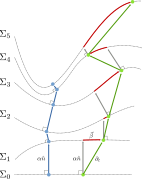
\includegraphics[width=\textwidth]{adm-definitions/adm-definitions.pdf}
	\caption[
	ADM definitions, drawn with Inkscape, \exclusive
	]{
		Cartoon for
		demonstrating the slicing (foliation) of 1+1 spacetime.
		The fixing of gauge freedoms is arbitrary and the shown example
		follows by intention no standard gauge fixing choice in NR.
		The foliation geometry is defined in continuum, this cartoon
		shows a number of different spatial hypersurfaces $\Sigma_i$,
		an exemplary normal vector fieldline (blue) 
		as well as an exemplary coordinate fieldline (green), determined
		by the time vector, which decomposes into spatial (shift) and
		temporal (lapse) direction. The lapse is the only spatial vector
		(``living on $\Sigma_i$''), while the other shown vectors are
		temporal. Since the vectors are shown non-bended, they shall be
		understood as infinitesimal.
	}
	\label{fig:efe-intro-2body-paramspace}
\end{marginfigure}%

\subsection*{3+1 split of the Energy momentum tensor}\label{sec.3p1-emtensor}
The normal vector $n_\mu$ as well as the spatial metric $\gamma_{ij}$ are
suitable for projecting four dimensional tensors into purely spatial or
purely temporal objects. Before this ``split'' is applied to Einstein equations
(Section~\ref{sec:3p1-split-efe}), it shall be applied to the Einstein source,
\ie the energy momentum tensor $T_{\mu\nu}$. Following the standard definitions,
the following four quantities, all measured by the Eulerian observer, shall be
defined:
\begin{align}
\label{eq:smunu.E}
E&=n^\alpha n^\beta T_{\alpha\beta}
\quad&&\text{the energy (momentum) density,}
\\
\label{eq:smunu.Si}
S_\alpha &= -\gamma^\mu_\alpha n^\nu T_{\mu\nu}
~~&&\text{the energy (momentum) flux,}
\\
\label{eq:smunu.Sij}
S_{\alpha\beta} &= \gamma^\mu_\alpha \gamma^\nu_\beta T_{\mu\nu}
\quad&&\text{the spatial energy momentum tensor and}
\\
S &= S^i_i 
\quad&&\text{its trace.}
\end{align}

\subsection[ADM equations]{3+1 split of Einstein Equations: ADM 
equations}\label{sec:3p1-split-efe}
The ADM split of Einsteins field equations is most readily obtained by
projection operators applied on EFE written as $G_{\mu\nu} - 8\pi T_{\mu\nu} = 0$
with the Einstein tensor 
$G_{\mu\nu} = R_{\mu\nu} + \nicefrac 12 R g_{\mu\nu}$ and the
Energy-Momentum-Tensor $T_{\mu\nu}$. Then, a full projection onto the normal
direction yields the Hamiltonian constraint equation
%\begin{subequations}\label{eq:adm-system}
\begin{equation}\label{eq:adm-system.hamiltonian}
0 = n_\mu n_\nu (G_{\mu\nu} - 8\pi T_{\mu\nu} ) = R - \tr(K^2) + (tr K)^2 - 16\pi~E
:= H
\end{equation}
Similarly, the three momentum constraints are derived by the
mixed projection:
\footnote{The notation $v_\alpha=(0,w_a)$ shall indicate that the 
  left hand side is four dimensional, while the right hand side is a purely
  spatial vector.}
\begin{equation}\label{eq:adm-system.momentum}
0 = \gamma_{\alpha\beta} n_\gamma (G_{\alpha\gamma} - 8\pi T_{\alpha\gamma} )
  = \left( 0, \nabla_k K^k_a - \nabla_a \tr K - 8\pi ~ S_a \right)
  := M_a
\end{equation}
$H=0$ and $M_a=0$
are the Hamiltonian and Momentum constraints, respectively, and their
deviation from zero (due to numerically introduced errors) is a measure to
assess the physicality of a system state.

The full projection onto the spatial hypersurface gives an evolution equation
for the extrinsic curvature,%
%\footnote{
%  Here it is convenient to project the Ricci tensor (following York
%  \cite{York79}) instead of the Einstein tensor (as ADM did).
%}
\begin{align}\label{eq:adm-system.kextr}
&  \gamma_{\alpha\beta} G^{\alpha\gamma} =
  \gamma_{\alpha\beta} 8\pi T^{\alpha\gamma} 
  \quad\Leftrightarrow\quad
  %(\partial_t - \Lie_{\bf \beta})
  \Lie_{\boldsymbol n} K_{ij} = \mathcal E_{ij}
  \,,
  \\
  \text{with}\quad
&   \mathcal E_{ij} = 
  - \nicefrac 1\alpha \nabla_i \nabla_j \alpha + 
  R_{ij} - 2 K_{ij} K^k_j + K K_{ij}
  - 8\pi \left( 
  S_{ij}  - \frac 12 \gamma_{ij} (S-E) \right)
  \nonumber
  \,.
\end{align}
The definition $K_{\mu\nu} = -\nicefrac 12 \mathcal L_{\boldsymbol n} 
\gamma_{\mu\nu}$ is already the evolution equation for $\gamma_{ij}$,
\begin{equation}\label{eq:adm-system.gamma}
\mathcal L_{\boldsymbol n} \gamma_{ij} = -2 K_{ij} \,.
\end{equation}
%\end{subequations}
The two evolution equations in $n^\mu$ direction can be transformed to
evolution equations using the ``time'' introduced in the previous section,
\ie \eqref{eq:lie-normal}.

The four equations (\ref{eq:adm-system.hamiltonian}-\ref{eq:adm-system.gamma})
are generally known as ADM equations.
With their 1+3 constraint equations and 6 evolution
equations\footnote{$\gamma_{ij}$ and $K_{ij}$ are symmetric 3-tensors with
	6~DOF each, however they are conjugate variables and therefore hold the 
	same information.}, they have the same 10~DOF as Einstein 
	field equations.

It is worthwhile to emphasize at this point that the constraint equations can
be used as Lagrangian Multipliers, for instance was $H$ already 
introduced
as Lagrangian multiplier in
$\Lie_{\boldsymbol n} K_{ij} = \mathcal E_{ij} - \gamma_{ij} H$ by 
York~\cite{York79}.
Obviously this does not change (continuum) physics, but the PDE
structure (system matrix) is a different one.

The ADM evolution equations are only weakly hyperbolic. This can be seen by
rewriting them as a first order formulation, fixing the gauges and showing
that parts of the system are not diagonizable \cite{Alcubierre:2008}.
As discussed in Section~\ref{sec:intro-eigensystems}, weakly hyperbolic PDEs
are not suitable for numerical integration since they are not well-posed.

\subsection{Gauge fixing}\label{sec:gauge-fixing}
\begin{marginfigure}[-2cm]
	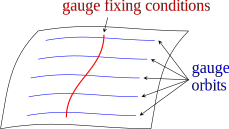
\includegraphics[width=\linewidth]{adm-gauge-orbits/gauge-orbits.pdf}
	\caption[Gauge orbits, \colorizedAfter{Meusburger:2010fs}
	]{
		Gauge fixing conditions must cut every gauge orbit 
		once. Every
		gauge orbit represents one physical solution which is 
		similar to
		another one. This generic sketch and language from 
		gauge theory can be
		mapped to GR/ADM language, a physical solution is a 
		particular
		coordinate system/slicing of spacetime.
		Colorized from~\cite{Meusburger:2010fs}.
	}
\end{marginfigure}%
In numerical relativity, gauge terms \emph{have} to be fixed since they appear
in the ADM system \eqref{eq:adm-system.kextr} and a numerical treatment requires
every variable to be represented by a number.

Physically, the effect of gauge fixing in the ADM split is equivalent to choose
a reference frame in GR (as it fixes the same four DOF). Fixing the lapse $\alpha$ determines the foliation and time coordinates
(``slicing conditions'') while fixing the shift $\beta^i$ chooses the spatial
coordinates. The gauge freedom can be
used to move coordinates in a desirable way throught the simulation domain which itself
can make the three-dimensional evolution equations more hyperbolic or more
elliptic \cite{Gourgoulhon2012}, but they can even be (dynamically) evolved
by a PDE and thus extend the overall evolution system\footnote{
 That means their PDEs neccessarily have to be taken into account when
 making an eigenanalysis of the particular 3+1 formulation of Einsteins
 equation (refering to modification of ADM equations, as presented
 in the subsequent sections).
}.

\subsection*{Slicing conditions}
Slicing conditions can be time-locally defined by constraining ADM quantities,
for instance the maximal slicing condition where $K^i_i = 0$. This maximises
the volume of the spatial hypersurface (hence the name) and has singularity
avoiding features, \ie $\alpha\to0$ when $t \to \infty$. It yields an
elliptic equation for the lapse $\alpha$ which makes it unsuitable for
time evolutions\footnote{This is because the elliptic equation 
	(which has no time derivatives) has to be solved at every timestep.
	There are however approximations by parabolic laws
	\cite{Shibata99a,Shibata_book:2016}.
}. Being maximal sliced is a property of a single hypersurface. In constrast,
slicing conditions which are defined via the lapse (or coordinates)
characterize a series of hypersurfaces and are not meaningful for single
hypersurfaces~\cite{Gourgoulhon2012}, because in general the lapse has no
meaning on a single hypersurface\footnote{However, given a prescribed
	gauge-fixing law, the lapse can \emph{be given} meaning even on a single
	hypersurface.
}

There is also the class of algebraic slicing conditions which directly determine
the lapse function and do not require to solve a (differential) equation
(at least not for constructing the initial data/initial slice). The most
simple example of this class is geodesic slicing, where $\alpha:=1$.
It got its name from the worldlines of Eulerian observers, which can be shown
to be geodesic. Their eigentime $\tau=t$ is equivalent to coordinate time.

Harmonic slicing is the most likely a gauge which is comparable to
Lorentz gauge ($\partial_\mu A^\mu=0$ with gauge field $A^\mu$ in 
electrodynamics and related field theories). It can be defined as imposing
the gauge $\nabla_\mu \nabla^\mu x^\alpha = 0$ on the coordinates. This
translates the Laplace equation $\nabla_\mu \nabla^\mu t=0$ in 3+1 formalism,
\ie the time coordinate has a harmonic solution. It is a special
case of $1+\log$/Bona Masso slicing, which is given by 
\cite{Bona95b}
\begin{equation}\label{eq:bona-masso}
(\partial_t - \Lie_\beta) \alpha = -(K-K_0) \alpha^2 f(\alpha)
\end{equation}
where $f(\alpha)=0$ gives geodesic slicing, $f(\alpha)=1$ gives harmonic
slicing and $f(\alpha)=2/\alpha$ gives ``1+log''-slicing, which gets it
name from the special case $\beta=0$ where \eqref{eq:bona-masso} reduces
to $\partial_t \alpha=\partial_t \ln |\gamma|$ which has the solution
$\alpha=1+\ln |\gamma|$. 1+log slicing has even better singulatiry avoidance
properties then harmonic slicing but can penetrate horizons (in Schwarzschild
spacetime), furthermore it mimics maximal slicing. Here, a
formulation with $K_0=K(t_0)$ the extrinsic curvature trace at beginning of the
simulation is given, which can help to preserve maximally sliced initial
data. Most worth mentioning, \eqref{eq:bona-masso} is a hyperbolic
conservation law for the lapse, which makes it an interesting addition to
a 3+1 evolution system.

\subsection*{Spatial gauges}
Fixing the temporal gauge freedom $\alpha$ determines the arrow of time at any
spatial hypersurface, since time is defined differentially between spatial
hypersurfaces. Instead, fixing the three gauge freedoms $\beta^i$ determines only
the propagations of coordinates between the hypersurfaces but leaves the choice of
coordinates for instance at the initial data hypersurface undetermined. This is because
the gauge connections $(\alpha, \beta^i)$ are only meaningful
quantities \emph{inbetween} two spatial hypersurfaces\footnote{
	In fact, there exist also \emph{full} spatial coordinate-fixing choices but they
	are not discussed here.
}.

Similar to the geodesic slicing, there is the Eulerian gauge $\beta^i=0$ as then
$x^i=$const are the worldlines of an Eulerian observer. As soon as the spacetime
is non-static, better more tailored spatial coordinates might be wanted. One
example are minimal distortion gauges which try to minimize the change of the
(conformal) 3-metric.
They yield in an elliptic equation for the shift. However,
minimal distortion gauges are interesting for the wave zone in a merger event,
basically because they are adapted to the way how gravitational waves are defined
and extracted (Appendix~\ref{sec:extracting-gws}).

Most interesting for this monograph are the Gamma freezing and Gamma driver
shift conditions. The first one is a simplification of approximative (pseudo)
minimal distortion gauges and can be formulated as\footnote{
	Here, the tilde in $\tilde{\gamma}$ and $\tilde{\Gamma}$ indicate 
	\emph{conformal} quantities as introduced in Section~\vref{sec:bssn}.
	Especially, the contracted Christoffel symbol is an evolution quantity
	in the BSSNOK system.
}
\begin{equation}
\partial_t \tilde{\Gamma}^i = 0, \quad\text{with}~~
\tilde{\Gamma}^i := \tilde{\gamma}^{jk} \left(\tilde{\Gamma^i}_{jk} - \tilde{\Gamma^i}_{jk} \right)
\end{equation}
An elliptic equation for the shift can be derived which must be fulfilled. By
further modifying the minimal distortion law, a parabolic \cite{Alcubierre00a}
and eventually a hyperbolic \cite{Alcubierre02a,Lindblom:2003ad,Bona05a}
alternative has been found, which reads in first order 
formulation
\begin{equation}\label{eq:gamma-driver}
	\partial_t \beta^i = \frac 34 b^i + \beta^k \partial_k \beta^i
	\quad\text{and}\quad
	\partial_t b^i = \partial_t \tilde\Gamma^i - \eta b^i + \beta^k \partial_k 
	b^i
\end{equation}
with a positive function $k$, a dissipation/damping coefficient $\eta$ and $b^i$ the
auxilliary field required for the first order rewrite
\cite{Baker:2006mp,Brugmann:2008zz}. Typical values are $k=3/4$ and
$\eta=1$ or $\eta\sim M/M_0$ with $M$ the ADM mass measured in multiples of the
unit mass $M_0$ (\ie $M_0=\Msol$ in astrophysical spacetimes).

The gamma driver shift condition turned out to be very successful for moving puncture
solutions and is, as part of the BSSNOK equations as presented in the next section,
an ``industry standard'' for stable general relativistic evolutions of compact object
mergers.

\section{The BSSNOK equations}\label{sec:bssn}

The Baumgarte-Shapiro-Shibata-Nakamura-Oohara-Kojima
(BSSNOK) formulation \cite{Shibata95,Baumgarte99,Nakamura87,Brown09},
is a hyperbolic formulation of Einsteins Equations in the
3+1 split. Hyperbolicitiy is archived with several ``tricks'' added to the
ADM system. These are primarily a conformal transformation of the ADM
state variabels $\gamma_{ij}, K_{ij} \to \tilde{\gamma}_{ij}, \tilde A_{ij}$,
the addition of the constraint equations $H=M_i=0$ to the evolution equations,
the addition of slicing conditions and Gamma driver to the evolved equations
and the seperate evolution of several quantities such as the extrinsic curvature
trace $K$, a contracted Christoffel symbol and the conformal factor. The
evolved variables of the BSSNOK system are therefore
\begin{equation}\label{eq:bssnok-evol-quantities}
\begin{aligned}
&\gammat_{ij} := e^{-4\phi} \gamma_{ij}
\,,\quad\quad
\Atilde_{ij} := e^{-4\phi} \TraceFree{K_{ij}} :=
e^{-4\phi}
\left( K_{ij} - \frac 13 \gamma_{ij} K \right)
\,,
\\
&\Phi := \frac{1}{12} \ln(\gamma) 
\,,\quad
K  := \gamma^{ij} K_{ij}
\quad\text{and}\quad
\Gtilde^i := \gammat^{jk} \Gtilde^i_{jk}
\,,
\end{aligned}
\end{equation}
where $\gammat_{ij}$ is the conformal 3-metric,
\begin{equation}
\tilde{\Gamma}^i_{jk} := \frac{1}{2} \gammat^{ab} \left(
\partial_{j} \gammat_{kb} + \partial_k \gammat_{jb} - \partial_b \gammat_{jk}
\right)
\end{equation}
are the Christoffel symbols associated with this metric and $\tilde{\Gamma}^i$
the freely evolved contraction of this symbol. $\Phi$ is the conformal factor
(see Section~\ref{sec:conformal-factor}) split off
the metric. $\tilde A_{ij}$ is the conformal trace-free extrinsic curature tensor which
is evolved in place of $K_{ij}$. Furthermore, with suitable slicing conditions
and the Gamma driver, lapse $\alpha$, shift $\beta^i$ and an auxillary field $b^i$
is evolved.

\subsection{Covariance of the BSSNOK formulation}
All new evolution fields $\Psi, K, \tilde{\Gamma}^i$ are pure gauge quantities
\cite{Baumgarte99}. The scalars $\Psi$ and $K$ are derived from tensors,
however $\tilde{\Gamma}^i$ does not transform like a vector, since the connection
coefficients $\Gamma^i_{jk}$ do not. Therefore, the BSSNOK equations are not
(fully) covariant.
However, the difference between two Christoffel symbols in a coordinate change
transforms like a tensor field \cite{Gourgoulhon2012}. % P.243
That is, if one introduces a background metric $\mathring{\gamma}_{ij}$
and a new metric $\epsilon_{ij} = \tilde{\gamma}_{ij} - \mathring{\gamma}_{ij}$, then
the Christoffel symbols of the new metric,
$\Delta^i_{kl} = \tilde{\Gamma}^i_{kl} - \mathring{\gamma}^i_{kl}$
and the derived $\hat{\mathring\Gamma}^i$ does so, too.
For BSSNOK, a system like this was introduced in \cite{Ruchlin2017} in 
order to evolve Einstein field equations on spherical and singular coordinate systems.
\footnote{Appendix \ref{sec:fo-fccz4} deepens this issue for the presented
  FO-CCZ4 formulation in this chapter.}

\subsection{Definitions for the conformal factor}%
\label{sec:conformal-factor}
% section comes from my document 
%Antelope/doc/conformal-treatment.pdf

A key concept in BSSNOK is splitting off a conformal factor, recognizing
that the three-metric $\gamma_{ij}$ and three-extrinsic curvature $K_{ij}$
are part of a conformal equivalence class. Evolving a fundamental representation
does not only have an advantage in conformally flat spacetimes but in fact
it was shown by York \cite{York71,York72} that a traceless and tranverse
tensor carries the true degrees of freedom of the gravitational field
\cite{Gourgoulhon2012}. Therefore, the concept was picked up by various
other formulations of Einsteins equations and especially by various
technical implementations, sometimes with subtle differences in the definition,
usually due to technical reasons (like positivity preserving techniques) which 
promise better numerical stability. In order to clarify the definitions, some
intermediate symbols shall be defined. First of all, any (rank 2)
tensor, for instance the 3-metric $\gamma_{ij}$, has a corresponding tensor 
density $\gammat_{ij}=\gamma^{n/2}\gamma_{ij}$ with weight $n\in\mathbb R$
and determinant $\gamma=\det(\gamma_{ij})$~\cite{Gourgoulhon2012}. The weight of
the three metric is $n=2/3$ and therefore, the conformal factor $\Omega$ can be
introduced as
\begin{equation}
\Omega = \gamma^{1/3}
\quad\text{so that}\quad \gamma_{ij} = \Omega ~ \gammat_{ij}
\end{equation}
In literature, the notation $\psi^4 \equiv \Omega$ is more widespread
\footnote{to be explicit, in $\psi^4$, the~$\cdot^4$ is an exponent, not an 
index. This symbol should not be mixed up with the Weyl scalar $\psi_4$,
where the $\cdot_4$ is really an index.% The Weyl scalar is popular in
%numerical relativity for extracting gravitational waves
%(Appendix~\vref{sec:extracting-gws}).
}, thus
$\gamma = \psi^{12}$. The following three popular but different choices are
widespread in literature
\footnote{This choice is motivated due to the implementation of all three
 variants in the \code{Antelope} code (see Section \vref{sec:fo-ccz4-implementations}).
}, formalized by a function $f(\Omega)$, or $f(\psi^4)$,
respectively. It is then $\gamma_{ij} = f^{-1} ~ \gammat_{ij}$. The three
choices $f\in\{ \xi, \Phi, W \}$ are\footnote{
  Within the BSSNOK community, the choice $f=\Phi$ is popular (and was
  made here in the text), while for instance \cite{Shibata_book:2016}
  uses $f=W$ and \cite{Hilditch2012} uses $f=\xi$.
}
%
%\begin{subequations}
\begin{alignat}{8} % was 10
\xi (\Omega) &= \Omega^{-1}  &&= \psi^{-4} &&= \gamma^{-1/3} \,,
&&\quad\text{then}~~ \gamma_{ij} = \xi^{-1}~ \gammat_{ij}
%&&\quad \texttt{(ifdef XI)} 
\label{eq:conformal-factor-Xi}
\\
\Phi  (\Omega) &= \log \Omega^3 &&= \log \psi &&= \frac 1{12} \log \gamma \,,
&&\quad\text{then}~~ \gamma_{ij} = e^{4\Phi}~ \gammat_{ij}
%&&\quad \texttt{(ifdef PHI)}
\label{eq:conformal-factor-Phi}
\\
W     (\Omega) &= \Omega^{-1/2} &&= \psi^{-2} &&= \gamma^{-1/6} \,,
&&\quad\text{then}~~ \gamma_{ij} = W^{-2}~ \gammat_{ij}
%&&\quad \texttt{(default)}
\label{eq:conformal-factor-W}
\end{alignat}
%\end{subequations}
%
However, the choice of a particular $f$ does not necessarily mean that this 
quantity
is evolved. In fact, the notation used for the FO-CCZ4 system
(Section~\ref{sec:fo-ccz4}) uses choice \eqref{eq:conformal-factor-W}
but calls $W(\Omega) =: \phi$. However, $\phi$ is treated as a
\emph{primitive} variable which is converted to a \emph{conserved}
variable where $\log \phi = \log W = - \nicefrac 16 \log \gamma$, which however
does not meet any standard definitions of
(\ref{eq:conformal-factor-Xi}-\ref{eq:conformal-factor-W})

\subsection[Evolution equations]{The BSSNOK evolution equations}
The BSSNOK equations are given by (see \cite{Brown09} for a derivation)
\begin{fullwidth} % tufte
%	\begin{subequations}
		\begin{align}
		\label{eq:bssn-phi}
		\left(\partial_t - \Lie_{\beta} \right) \Phi
		&=
		\frac 16 \partial_k \beta^k - \frac 16 \alpha K
		\\
        \label{eq:bssn-gammat}
		\left(\partial_t - \Lie_{\beta} \right) \gammat_{ij}
		&=
		-2\alpha \Atilde_{ij} - \frac 23 \gammat_{ij} \partial_k \beta^k
		\\
        \label{eq:bssn-K}
		\left(\partial_t - \Lie_{\beta} \right) K
		&=
		\alpha \left( \Atilde_{ij} \Atilde^{ij} + \frac 13 K^2 \right)
		- \gamma^{ij} \nabla_i \nabla_j \alpha
		+ 4\pi (S^k_k + E)
		\\
        \label{eq:bssn-Atilde}
		\left(\partial_t - \Lie_{\beta} \right) \Atilde_{ij}
		&=
		e^{-4\Phi} \TraceFree{\alpha(R_{ij} - 8\pi S_{ij}) - \nabla_i \nabla_j 
		\alpha}
		- \frac 23 \Atilde_{ij} \partial_k \beta^k + \alpha \left(K 
		\Atilde_{ij} - 2\Atilde_{ik} \Atilde^k_j \right)
		\\
        \label{eq:bssn-Gtilde}
		\left(\partial_t - \Lie_{\beta} \right) \Gtilde^i
		&=
		\gammat^{kl} \partial_k \partial_l \beta^i
		+ \frac 23 \gammat^{jk} \Gtilde^i_{jk} \partial_l \beta^l
		+ \frac 13 \nabla^i \partial_k \beta^k
		- 2 \Atilde^{ik} \partial_k \alpha
		%\\
		%&\phantom{=}
		+ 2 \alpha \Atilde^{kl} \Gtilde^i_{kl}
		+ 12 \alpha \Atilde^{ik} \partial_k \phi
		- \frac 43 \alpha \tilde\nabla^i K
		- 16\pi \alpha \gammat^{ij} S_j
		\raisetag{32pt}
		\\
        \label{eq:bssn-alpha}
		\left(\partial_t - \Lie_{\beta} \right) \alpha
		&=
		-2 \alpha K
		\\
        \label{eq:bssn-beta}
	    (\partial_t - \Lie_{\beta}) \beta^i
		&=
		\frac 34 b^i
		\\
        \label{eq:bssn-auxB}
	    (\partial_t - \Lie_{\beta}) b^i
		&=
		\partial_t \Gtilde^i - \eta b^i
		\end{align}
%	\end{subequations}
\end{fullwidth}
with the covariant derivative $\tilde{\nabla}$ with respect to $\gammat_{ij}$
\footnote{Here, only terms $\tilde{\nabla}_i A=\partial_i A$
	and $\tilde{\nabla}_i B_j = \partial_i B_j - \tilde{\Gamma}^k_{ij} B_k$ appear.
},
Lie derivative $\Lie_{\beta} = \beta^k \partial_k$\footnote{
	Conventionally, the ADM system is typically displayed as
	$\Lie_{\boldsymbol{n}} X = \mathcal R(X)$ while the BSSNOK and 
	subsequent systems are typically displayed as
	$(\partial_t - \Lie_{\beta}) X = \alpha \mathcal R(X)$.
}, the trace-free operator $\TraceFree{T_{ij}}$ defined as in 
\eqref{eq:bssnok-evol-quantities}, and $(E,S_i,S_{ij})$ being 
the spatial parts of the energy momentum tensor as defined in
(\ref{eq:smunu.E}-\ref{eq:smunu.Sij}). In this equation system, there
are especially two very lengthy abbreviations used: First, the
3-Ricci tensor in \eqref{eq:bssn-Atilde} which is defined with the conformal
decomposition $R_{ij} := \tilde R_{ij}^\Phi + \tilde R_{ij}$ as%
\footnote{Elaborate splits of ``helper'' quantities (\ie tensors derived from
evolution quantities) will become even more present in the FO-CCZ4 system.}
\begin{align}\label{eq.bssnok.conformalR}
\tilde R_{ij}^\Phi 
&=
\Phi^{-2} \left[
\Phi \left( \tilde\nabla_i \tilde\nabla_j \Phi
+ \gammat_{ij} \tilde\nabla^k \tilde\nabla_j \Phi \right)
- 2 \gammat_{ij} \tilde\nabla^k \tilde\nabla_k \Phi \right] \,,
\\
\tilde R_{ij}
&=
- \frac 12 \gammat^{lm} \partial_l \partial_m \gammat_{ij}
+ \gammat_{k(i} \partial_{j)} \Gtilde^k
+ \Gtilde^k \Gtilde_{(ij)k} + \gammat^{lm}
\left[ 2 \Gtilde^k_{l(i} \Gtilde_{j)km} 
+ \Gtilde^k_{im} \Gtilde_{kjl} \right] \,,
\nonumber
\end{align}
and second, the time-derivative of $\tilde{\Gamma}^i$ in \eqref{eq:bssn-auxB}
which refers to \eqref{eq:bssn-Gtilde}.

The evolution system also contains PDEs for the lapse $\alpha$ and shift
vector $\beta^i$, in this particular case the famous Bona-Masso type slicing
conditions.

For the numerical intergration, a partly constrainted approach is used at every
time step to impose that \footnote{In practice, this means a modification of 
 the state vector before or after every timestep.}
\begin{equation}
\det(\gammat_{ij}) = 1 \quad\text{and}\quad \operatorname{tr}(\Atilde_{ij}) = 0
\end{equation}
Similiar to ADM equations, the BSSNOK system is first order in time and second
in space, for a proof of hyperbolicity it must be brought into first order in
time and space (this was done in \cite{Beyer:2004sv} for a large number of
slicing conditions). Notably, for a fixed (non-evolved) shift vector
$\beta^i$, BSSNOK is symmetric hyperbolic. Since its first publication,
BSSNOK was quite successful for its robustness in numerical simulations and
got an ``industry standard'' for numerical relativistic time evolutions of
astrophysical spacetimes.

%Note the added Hamiltonian and momentum constraints on the RHS in order to
%guarantee hyperbolicity of the system.

%In the same publication, a different definition of hyperbolicity
%also proofs the second order version of BSSNOK strongly hyperbolic for any
%shift condition.

\section{The Z4 family and CCZ4}\label{sec:Z4-family}
The Z4 formulation of Einstein field equations (EFE) was formulated by Bona,
Ledvinka, Palenzuela, Zacek \cite{Bona:2003fj,Bona:2003qn}. They recognize that
in ADM formalism, the discrimination of the constraint equations
(\ref{eq:adm-system.hamiltonian},\ref{eq:adm-system.momentum}) versus the 
evolution equations
(\ref{eq:adm-system.kextr},\ref{eq:adm-system.gamma})
in a ``naive'' unconstrained evolution breaks general covariance. In Z4,
the derivative of a zero vector $Z_\mu=0$ \footnote{$Z_\mu=0$ motivates the 
name: A ``zero'' vector of length 4,	hence ``Z4''. The vector vanishes 
analytically but gets non-zero in numerical simulations.} is added to the field 
equations as a generalized Lagrangian multiplier (GLM)
which then read in trace-reversed form \cite{Bona:2003fj}
\begin{equation}\label{eq:z4-efe}
R_{\mu\nu} + 2\nabla_{(\mu} Z_{\nu)} = 8\pi \left( T_{\mu\nu} - \frac 12 T 
g_{\mu\nu} \right) \,.
\end{equation}
The field equations can also be derived from a minimal action principle
\cite{Bona:2010is}. They are first order in time, second order in space for the
metric, first order in space for $Z_\mu$. 
\footnote{The actual evolution equations are given later compact for all
	proposed members of the Z4 family.}
In the 3+1 split, with $Z_\mu = (\theta / \alpha, Z_i)$, the two new
evolution quantities for $\theta$ and $Z_i$ cannot be discriminated against
the ones for $\gamma_{ij}$ and $K_{ij}$ and thus general covariance is
maintained. Notably, these two new evolution equations take the place of the
ADM constraint equations, because $Z_\mu=0$ are four constraints and
non-zero values of $Z_\mu$ measure the ``physicality'' of an approximated
(numerical) solution. This is  a \emph{different} measure for
error than the regular
ADM Hamiltonian and momentum constraint (violations)
(\ref{eq:adm-system.hamiltonian},\ref{eq:adm-system.momentum}) which of course
still can be determined similarly also in the Z4 system, independently
of the $Z_\mu$ vector \footnote{For a comparison of the quality of 
 different formulations of EFEs, it is
 useful to fall back to $(H,M_i)$ as the ``lowest common denominator'',
 which always can be computed.}. The resulting PDE system is then almost similar
to the ADM equations (\ref{eq:adm-system.hamiltonian}-\ref{eq:adm-system.gamma}), namely
\begin{fullwidth}% tufte
\begin{align}
	\left(\partial_t - \Lie_{\beta} \right) \gammat_{ij}
	&=
	-2\alpha K_{ij}
	\\
	\left(\partial_t - \Lie_{\beta} \right) K_{ij}
	&=
	-\nabla_i \nabla_j \alpha
	+ \alpha \left[ R_{ij} - 2 K_{ij} K^k_j + (K-2\Theta)K_{ij}
	%- \NewTerms{\kappa_1(1+\kappa_2)\Theta\gamma_{ij}}
	\right]
	%\\
	%&\phantom{=}
	- 8\pi\alpha \left[ S_{ij} - \frac 12 \gamma_{ij} (S-E) \right] 
	\\
	\left(\partial_t - \Lie_{\beta} \right) \Theta
	&=
	\frac \alpha 2 \left[
	R + 2 \nabla_k Z^k + (K - 2\Theta)K - K_{ij} K^{ij}
	\right]
	- Z_k \nabla_k \alpha  
	% -\NewTerms{2\kappa_1(2+\kappa_2)\Theta} 
	- 16 \pi E
	\\
	\left(\partial_t - \Lie_{\beta} \right) Z_i
	&=
	\alpha \left[ \nabla_j (K_i^j - \delta_i^j K)
	+ \partial_i \Theta - 2 K_i^j Z_j \right]
	- \Theta \nabla_i \alpha
	% - \NewTerms{\kappa_1 Z_i}
	- 8\pi S_i
	\end{align}
\end{fullwidth}
%
The first order version of Z4 was brought into a conservative form and is
proven to be strongly hyperbolic~\cite{Alic:2009}.
The main drawbacks of the Z4 formulation is the lack of the 
Gamma driver
\eqref{eq:gamma-driver}, \ie there are no good gauges which 
result in horizon 
growth in black hole simulations.

% Recovery of BSSNOK and KST is possible \cite{Kidder01a}
%
\subsection[Z4c]{Conformal Z4 (Z4c)}
The conformal Z4 (Z4c) version was developed as a conformal but non-covariant
extension to Z4 \cite{Bernuzzi:2009ex,Cao:2012,Ruiz:2010qj,Weyhausen:2011cg,Hilditch2012}.
The modified EFEs
\begin{equation}\label{eq:Z4c}
R_{\mu\nu} + 2\nabla_{(\mu} Z_{\mu)}
=
8\pi (T_{\mu\nu} - \frac 12 T g_{\mu\nu})
+ \kappa_1 \left[ 2 n_{(\mu} Z_{\nu)} - (1 + \kappa_2) g_{\mu\nu} n_\sigma Z^\sigma \right]
\end{equation}
differ from the Z4 equations \eqref{eq:z4-efe} only by the algebraic damping
terms on the RHS, modulated by $\kappa_1$ and $\kappa_2$ which determine the damping
amplitude used to drive the growth of constraint violations to zero.
In the 3+1 split the Z4c formulation discard a number of terms which renders the
evolution equations non-covariant but very close to BSSNOK.
\todo[color=green]{
    Z4c: It would be nice to better work out the differences between Z4c and CCZ4.
    Especially since we have Z4c implemented in Antelope, also the practical difference
    is of interest, such as cost, Exactness. This would all be part of the frequently
    discussed code comparison paper which is however out of scope in the moment.
}
The resulting system is provably strongly hyperbolic for usual gauge choices.

The addition of the damping terms allows to advect and (if desired) damp
nonzero constraints which appeared during evolution. The consequence is of
course that the numerical solution stays much closer to a physical one, which is
especially helpful for very long running simulations (compared to the average
wave speed, \ie the speed of light, or the  mass of the spacetime, respectively).
The typical text-book motivation for this
mechanism employs Gauss law in electromagnetism, \ie preserving the solenoidal magnetic
field $\vec \nabla \cdot \vec B=0$, where the GLM is introduced as \cite{Dedner:2002}
\begin{alignat}{3}
\partial_t B^i &= \mathcal  R
&&\quad\Rightarrow\quad  \partial_t B^i = \mathcal R - \partial^i \psi \\
\partial_i B^i &= 0
&&\quad\Rightarrow\quad  \partial_i B^i = \mathcal  D(\psi) = 
c_\text{cleaning}^{-2} \partial_t \psi
\end{alignat}
In this minimal example, there is an evolution equation for the vector $B^i$ 
with a
spatial differential operator $\mathcal R = \mathcal R(B^i, \partial_i B^j, 
\dots)$.
The new evolved scalar $\psi$ couples the divergence freedom ($\partial_i 
B^i=0$)
to the evolution equation, following a differential operator $\mathcal D$. A 
hyperbolic
choice for this operator results in an advection quation for $\psi$.
~In a similar way, in Z4c, the four fields $(\Theta,Z_i)$ play the role of $\psi$
in this example.\footnote{
  See section \ref{sec:divergence-cleaning} for divergence cleaning
  techniques in magnetohydrodynamics.
}

%$\partial_i A^i = 0$ becomes instead $\partial_t A^i = \phi$ and
%$\partial_t \phi = \partial_t A^i$

\subsection[SO-CCZ4]{Conformal and covariant Z4: (SO-)CCZ4}
The CCZ4 (conformal and covariant Z4) system was developed to address
the non-covariant property of Z4c~\cite{Alic:2011a}. The derivation starts with 
the same field equations \eqref{eq:Z4c} but do not discard terms at the 3+1 split.
\footnote{
  Thus, the property ``covariant'' in CCZ4/Z4c is to be understood as
  ``beeing \emph{more} covariant then Z4''. However, as CCZ4 takes over the
  non-covariant ``conformal connection functions'' $\tilde{\Gamma}^i$ from
  BSSNOK (Section \ref{sec:bssn}), CCZ4 is not covariant.
  Appendix \ref{sec:fo-fccz4} briefly presents a \emph{fully} covariant CCZ4
  system which implements the ideas of \cite{Ruchlin2017}.
}

The conformal transformation applied in CCZ4 is similar to the BSSNOK one but
usually given with a different conformal factor (here $f=W$ from 
Section~\ref{sec:conformal-factor}),
\begin{equation}
\begin{aligned}
W      &:=  \gamma^{-\nicefrac 16}  \,,
&
K      &:=  \gamma^{ij} K_{ij}  \,,
\\
\gammat_{ij}  &:= W^2 \gamma_{ij}  \,,\quad
&
\Atilde_{ij}  &:= W^2 \TraceFree{K}  \,,
\\
\Gtilde^i     &:= \gammat^{jk} \Gtilde^i_{jk}  \,,
&
\Ghat^i       &:= \Gtilde^i + 2 \gammat^{ij} Z_j   \,,
\end{aligned}
\end{equation}
In CCZ4, the new symbol $\hat{\Gamma}^i$ replaces $Z_i$ as evolution quantity, while
$\Theta=Z_0$ remains an evolution quantity.

%
The full CCZ4 system in 3+1 split is given by
\cite{Alic2013,Alic:2011a}
\begin{fullwidth}
\begin{eqnarray}
%
\partial_t\tilde\gamma_{ij} &=& - 2\alpha \tilde A_{ij}
+ 2\tilde\gamma_{k(i}\partial_{j)}~\beta^k
- \frac{2}{3}\tilde\gamma_{ij}\partial_k~\beta^k
+\beta^k \partial_k \tilde\gamma_{ij} \,,  \label{gamma_eq}\\
%
\partial_t \tilde A_{ij} &=& \phi^2  \left[-\nabla_i \nabla_j 
\alpha
+ \alpha \left(R_{ij} + \nabla_i Z_j + \nabla_j Z_i - 8 \pi S_{ij}
\right)\right]^{\rm TF}
+ \alpha \tilde A_{ij}\left(K- 2\Theta\right) \nonumber \\
&&
- 2\alpha \tilde A_{il}\tilde A^l_j %\nonumber  \\
+ 2\tilde A_{k(i}\partial_{j)}~\beta^k
-\frac{2}{3}\tilde A_{ij}\partial_k~\beta^k + \beta^k 
\partial_k \tilde A_{ij}  \,,  \label{A_eq} \\
%
\partial_t\phi &=& \frac{1}{3} \alpha \phi K
- \frac{1}{3} \phi \partial_k \beta^k + \beta^k \partial_k \phi 
\,, \label{phi_eq} \\
%
\partial_t K &=& - \nabla^i \nabla_i \alpha + \alpha \left(R + 2
\nabla_i Z^i + K^2 -2 \Theta K \right)
+ \beta^j \partial_j K - 3 \alpha \kappa_1 \left(1 +
\kappa_2\right) \Theta  + 4 \pi \alpha \left(S - 3 \tau\right)
\,, \\
%
\partial_t \Theta &=& \frac{\alpha}{2}  \left[R + 2 \nabla_i 
Z^i - \tilde A_{ij} \tilde
A^{ij} + \frac{2}{3} K^2 - 2 \Theta K\right] - Z^i
\partial_i \alpha+ \beta^k \partial_k \Theta
- \alpha \kappa_1 \left(2 + \kappa_2\right) \Theta  - 8\pi 
\alpha\,\tau
\,,
\phantom{aaa}% avoid the tag to be ontop of tau
\\
%
\partial_t \hat\Gamma^i &=& 2\alpha \left[\tilde\Gamma^i_{jk} 
\tilde A^{jk}
- 3 \tilde A^{ij} \frac{\partial_j \phi}{\phi} - \frac{2}{3}
\tilde\gamma^{ij} \partial_j K \right]
+2\tilde\gamma^{ki}\left(\alpha \partial_k \Theta - \Theta
\partial_k \alpha
- \frac{2}{3} \alpha K Z_k\right) -  2\tilde A^{ij} \partial_j 
\alpha
\nonumber \\
&& + \tilde\gamma^{kl} \partial_k \partial_l \beta^i
+ \frac{1}{3}\tilde\gamma^{ik}\partial_k\partial_l \beta^l
+ \frac{2}{3} \tilde\Gamma^i \partial_k \beta^k -
\tilde\Gamma^k \partial_k \beta^i
+ 2 \kappa_3 \left(\frac{2}{3} \tilde\gamma^{ij} Z_j \partial_k 
\beta^k -
\tilde\gamma^{jk} Z_j \partial_k \beta^i \right)
\nonumber \\
&&  + \beta^k \partial_k \hat\Gamma^i 
- 16 \pi \alpha  \tilde\gamma^{ij} S_{j}
- 2 \alpha \kappa_1 \tilde \gamma^{ij} Z_j
\,, \label{Gamma_eq}
\\
%
\label{1plog}
\partial_t \alpha &=& - \alpha^2 g(\alpha) \left(K - K_0 - 
2\Theta \right) + \beta^k \partial_k \alpha \,, \\
%
\label{gammadriver1}
\partial_t \beta^i &=& f b^i +\beta^k\partial_k\beta^i \,, \\
%
\label{gammadriver2}
\partial_t b^i &=& \partial_t \hat\Gamma^i - \beta^k \partial_k 
\hat\Gamma^i
+ \beta^k\partial_k b^i - \eta b^i \,,
\end{eqnarray}
\end{fullwidth}
Here, again, the Gamma driver and Bona-Masso slicing conditions were added,
as in the case for the BSSNOK equations.

\section{The first order CCZ4 equations (FO-CCZ4)}\label{sec:fo-ccz4}
The first order (FO) rewrite of the second order (SO) CCZ4 system, as
introduced in the previous section, is a neccessary step for proving the
hyperbolicity of the SO-CCZ4 system as well as its implementation with
finite volume (Section~\vref{sec:fv}) or finite element
(Section~\vref{sec:dg}) schemes. The derivation of this big PDE system
is elaborate and it takes a full page to write down the PDE system with
all the helper quantities itself. A short version of the derivation
is part of our publication \cite{Dumbser2017}.

\subsection[Auxilliary variables, ordering constraints]
  {Introduction of the auxiliary variables and resulting ordering constraints}

The following 33 auxilliary variables are introduced, in order to collect
first spatial derivatives of metric terms,
\footnote{
   The naming and definitions 
   of these variables follows conventions seen in previous papers.
   For instance, the Z4 paper \cite{Bona:2003fj} defines already
   $A_k$ and $D_{kij}$ in a first order reduction of the Z4 equations
   to prove symmetric hyperbolicity in harmonic slicing. In that paper,
   the choices (like the logarithm in $A_i$ and the factor $\nicefrac 12$ in
   the definition of $D_{kij}$) were probably due to shortness of notation,
   while here we define $A_i$ as the derivative of the logarithm for means
   of positivity preserving (more on this in the main text).
}
%
\begin{equation}
\begin{aligned}
\label{eq:Auxiliary}
A_i &:= \partial_i\ln\alpha = \frac{\partial_i \alpha }{\alpha}\,, \qquad
&&&
B_k^{i} &:= \partial_k\beta^i\,,
\\
D_{kij} &:= \frac{1}{2}\partial_k\tilde\gamma_{ij}\,, \qquad
&&&
P_i       &:= \partial_i\ln\phi = \frac{\partial_i \phi}{\phi}\,.
\end{aligned}
\end{equation}
%
An immediate consequence of \eqref{eq:Auxiliary} and the Schwarz theorem
on the symmetry of second-order derivatives are the following second
order ordering constraints \cite{Gundlach:2005ta}, which read:
\begin{align}
\label{eqn.second.ord.const}
 \mathcal{A}_{ki}   &:= \partial_k A_i - \partial _i A_k        = 0\,, &
 \mathcal{B}_{kl}^i &:= \partial_k B_l^i - \partial_l B_k^i     = 0\,, \nonumber \\
 \mathcal{D}_{klij} &:= \partial_k D_{lij} - \partial_l D_{kij} = 0\,, &
 \mathcal{P}_{ki} &:= \partial_k P_i - \partial _i P_k = 0\,.
\end{align}
%
Since $\tilde{A}_{ij}$ is by construction trace-free, the following
additional constraint holds: $\tilde{\gamma}^{ij} \tilde{A}_{ij} = 0$,
and thus
\begin{equation}
\label{atf.diff}
\mathcal{T}_k := \partial_k \left( \tilde{\gamma}^{ij} \tilde{A}_{ij} \right) = \partial_k \tilde{\gamma}^{ij} \tilde{A}_{ij} + \tilde{\gamma}^{ij} \partial_k \tilde{A}_{ij} = 0. 
\end{equation}
These relations will be important later on in order to derive a
\textit{strongly} hyperbolic system in first-order form.
%
Furthermore, from the constraint $\det(\tilde{\gamma}_{ij}) =1$ and via
the Jacobi formula
\begin{equation}
 \partial_k \det(\boldsymbol{A}) = {\rm tr}(
\det(\boldsymbol{A}) \boldsymbol{A}^{-1} \partial_k \boldsymbol{A})
\end{equation} 
%% or in component form: $\partial_k \det(A) = \det(A) \gamma_i^j A^{il}
%% \partial_k A_{lj}$ 
on the derivatives of the determinant of a matrix, the
following additional algebraic constraints on the auxiliary variables
$D_{kij}$ is obtained (see also~\cite{Brown2012}):
%
\begin{equation} 
  \tilde{\gamma}^{ij} D_{kij} = 0\,. 
	\label{eqn.dcons} 
\end{equation} 
%
From Eq. \eqref{eqn.dcons}, another differential constraint follows,
namely, 
%
\begin{equation}
\partial_l \tilde{\gamma}^{ij} D_{kij} + \tilde{\gamma}^{ij} \partial_l
D_{kij}=0\,.
\end{equation}
%
In practical implementations, however, we have not found particular
benefits from making use of this additional constraint in the FO-CCZ4
formulation.

%
The evolution equations for the auxiliary quantities are obtained by
applying the temporal derivative operator $\partial_t$ to equations
\eqref{eq:Auxiliary}, by subsequently exchanging the spatial and temporal
derivatives on the right-hand side of the resulting equations and by
making use of the PDEs for $\tilde{\gamma}_{ij}$ \eqref{gamma_eq}, 
$\phi$ \eqref{phi_eq}, $\alpha$ \eqref{1plog} and $\beta^i$ 
\eqref{gammadriver1}.

Many different first-order formulations of the CCZ4 system are possible,
since any non-purely algebraic term in the original second-order system
can be written as a combination of conservative terms and
non-conservative products (see \cite{Gundlach:2005ta, Hilditch2015} for a
parametric study of such families of systems).

Two extreme cases stand out:
First, write as many terms as possible are written in a conservative
flux-divergence form (Eq. \ref{intro:balance-law}, but with a source
term that contains derivatives). For the first-order Z4
system, this was done in \cite{Alic:2009}.

Second, similar to the ideas outlined in
\cite{Alcubierre:2008}, making maximum use of the first-order ordering
constraints, so that the variables defining the 4-metric ($\alpha$,
$\beta^i$, $\phi$ and $\tilde{\gamma}_{ij}$) are only evolved by a
nonlinear system of ordinary differential equations (ODEs) and where the
rest of the dynamics is written in terms of non-conservative products
(Section \ref{sec:ncp}).
The coefficients of these non-conservative products are only functions of
$\alpha$, $\beta^i$, $\phi$ and $\tilde{\gamma}_{ij}$ and no differential
terms in these variables appear. The dynamical variables of the FO-CCZ4
system with Gamma-driver shift condition are then: $\tilde{A}_{ij}$, $K$,
$\Theta$, $\hat{\Gamma}^i$, $b^i$ (the $b^i$ vector is an auxiliary field
used to write the Gamma-driver gauge condition
\cite{Alcubierre:2008,Alic:2011a}) and the auxiliary variables $A_k$,
$B_k^i$, $P_k$ and $D_{kij}$.

We will follow the second
approach, \ie the final system of 58 evolution equations, evolving the
state vector
\begin{equation}\label{eq:foccz4-state-vector}
\boldsymbol Q_{FOCCZ4} = (\gamma_{ij}, K_{ij}, \Theta, \hat{\Gamma}_i, \alpha, \beta^i, b_i, A_i, B^i_j, 
D_{ijk}, K, \phi, P_k),
\end{equation}
which consist of
\begin{align}
	\label{eq:foccz4-ODE}
	\boldsymbol U &= (\gamma_{ij}, \alpha, \beta^i, \phi)
&\text{11 ODEs and} \\
	\boldsymbol V &= (K_{ij}, \Theta, \hat{\Gamma}_i, b_i, A_i, B^i_j, D_{ijk}, K, P_k)
	&\text{47 PDEs}
	\label{eq:foccz4-PDE}
\end{align}
and has a special structure discussed later in Section \ref{sec.hyp}.

\subsection{The FO-CCZ4 PDE system in the differential/algebraic 
split}\label{sec.foccz4}%
\todo[color=green,caption={FO-CCZ4: Check PDE system and colorize it}]{\footnotesize
	FO-CCZ4: The PDE system \ref{table.helpers.foccz4} should be checked for correctness
	against latest version. Then some color should be applied:
	(1) Conserved Fluxes
	(2) Constants (already done)
	(3) Symmetry terms
	(4) Matter terms
	(5) complex helper terms (such as Riemanns or $\nabla Z$ or $\nabla \alpha$)
}%
\begin{table*}[t]
	\makebox[\textwidth][c]{%
	 	%\includegraphics[width=1.2\textwidth]{astronum-ccz4-table/standalone-astronum-ccz4-table.pdf}
     	\scalebox{0.73}{\begingroup%% Common definitions require by both the CCZ4 system table as well
%% as the Riemann helpers table

%
%% Determine how to fix this...
%\setlength{\mathindent}{0pt}% amsmath, also require fleqn locally somehow
%
% left aligned vector
\newenvironment{pvector}{\begin{pmatrix*}[l]}{\end{pmatrix*}}%
%
% Wrap aligns inside the big CCZ4 table so the table can be
% put wiht background colors
\makeatletter%
\newcommand{\embedEQ}[1]{ {\CT@everycr{\the\everycr} #1 }}%
\makeatother%
%
% the parbox is important for getting a width
%\newcommand{\embedNCP}[1]{ \parbox{5cm}{\embedEQ{#1}} }
\newcommand{\longNCP}[1]{ \parbox{4.0cm}{\embedEQ{#1}} }%
\newcommand{\longSource}[1]{ \parbox{4.0cm}{\embedEQ{#1}} }%
%
\newcommand{\NCP}[1]{{\left[#1\right]_\text{NCP}}}%
\newcommand{\SRC}[1]{{\left[#1\right]_\text{SRC}}}%
%
% colorized CCZ4 parameters
\newcommand{\param}[1]{\textcolor{red}{#1}}%
% colorized CCZ4 matter sources
\newcommand{\matter}[1]{\textcolor{blue}{#1}}%
%
% define colors for CCZ4 variables
\definecolor{alpha}{HTML}{D1F2A5}%
\definecolor{beta}{HTML}{FFE3EB}%
\definecolor{gamma}{HTML}{FF9F80}%
\definecolor{phi}{HTML}{FFDFAB}%
%
\definecolor{Atilde}{HTML}{93DFB8} %FFC48C}
\definecolor{K}{HTML}{FFC8BA} %EFFAB4}
\definecolor{Theta}{HTML}{E3AAD6} %FFB397} % too dark: F56991
\definecolor{Gamma}{HTML}{B5D8EB} %EFFAB4}
\definecolor{b}{HTML}{FFBDD8} %CAE2D0}
%
\colorlet{A}{alpha}%
\colorlet{B}{beta}%
\colorlet{D}{gamma}%
\colorlet{P}{phi}%
%
% leftovers:
%\definecolor{D}{HTML}{FFB397}
\definecolor{varPP}{HTML}{DCEBFA}%
\definecolor{varK0}{HTML}{FCF3CD}%
%\definecolor{K}{HTML}{84C1FF}
%
\newcommand{\einefarbe}[1]{#1}%
%
% background colors
% yields errors:
\newcommand{\colorSymbol}[1]{ \cellcolor{#1} }%
\newcommand{\colorNCP}[1]{ \cellcolor{#1!50!white} }%
\newcommand{\colorSource}[1]{ \cellcolor{#1!60!white} }%
%
% Rotate text in multirow table (source: https://tex.stackexchange.com/a/89116)
\newcommand{\verticalrow}[2]{\parbox[t]{2mm}{\multirow{#1}{*}{\rotatebox[origin=c]{90}{#2}}}}%
%
% Integrals with long limits above/below
\newcommand{\Int}[2]{\int\limits_{\mathrlap{#1}}^{\mathrlap{#2}}}%
%
% This fully works, but of course makes one equation per
% 
\providecommand{\eqnNum}[2]{%
%%\addtocounter{equation}{1}% works, but instead use refstepcounter for label
%%
%% Works, but disabled for the time being for display
%\makeatletter%
%\def\@currentlabel{#2}%
%\renewcommand{\theequation}{\arabic{equation}.#2}%
%\makeatother%
%%
%%
\refstepcounter{equation}%%%\label{#1} % This line works, keep it!!!
\latexlabel{#1}% Using \latexlabel instead of label for tufte.
(\theequation)% mimic the display of an equation
}%
%
% the same but with subequtions...
\providecommand{\subEqnNum}[2]{%
	%\addtocounter{equation}{1}% works, but instead use refstepcounter for label
	%
	% test currentlabel thing
%	\makeatletter%
%	\def\@currentlabel{#2}%
%	\renewcommand{\thesubequation}{\themainequation.#2}%
%	\makeatother%
	% redefine \theequation
	%
	\refstepcounter{subequation}\label{#1} % This line works, keep it!!!
	(\theequation)% mimic the display of an equation
}%
%
%
\newcommand{\setAstronumTableSizes}{
\setlength{\abovedisplayskip}{3pt}%
\setlength{\belowdisplayskip}{3pt}%
\setlength{\abovedisplayshortskip}{3pt}%
\setlength{\belowdisplayshortskip}{3pt}%
}%%
% This is an attemp to graphically display the CCZ4 equations
% in a fancy way. It is rendered as standalone latex because
% there are so many tricks that this can be seen as a "Tikz-like"
% figure.
%
% This is a tex file supposed for inclusion.
% Make sure you include common-definitions.tex before including this file.
% For a standalone version, see standalone-astronum-ccz4-table.tex.
%
%\begingroup % group of no spacing around align environments
\setAstronumTableSizes
\begin{tabular}{lllll}
\toprule
& $Q_i$ & Nonconservative product NCP$_a(Q) = B^{ib}_a(Q) \partial_i Q_b$ & 
Algebraic 
source $S_{a}(Q)$ & Eqn. \\
\midrule
\verticalrow{6}{ODE-ADM}
& \colorSymbol{alpha} $\ln \alpha$
& \colorNCP{alpha} \longSource{\begin{equation*}
0
\end{equation*}}
& \colorSource{alpha} \longSource{\begin{equation*}
{ \beta^k A_k } - \alpha \param{g}(\alpha) ( K - K_0 - 2\Theta {c} )
\end{equation*}}
& \colorSymbol{alpha} \eqnNum{eq.foccz4.alpha}{$\alpha$}\label{eq.foccz4.alpha}  \\
%
%
& \colorSymbol{beta} $\beta^i$
& \colorNCP{beta} \longSource{\begin{align*}
0
\end{align*}}
& \colorSource{beta} \longSource{\begin{equation*}
\param s \beta^k B_k^i + \param s \, \param f \, b^i
\end{equation*}} 
& \colorSymbol{beta} \eqnNum{eq.foccz4.beta}{$\beta$}  \\
%
%
& \colorSymbol{gamma} $\tilde \gamma_{ij}$
& \colorNCP{gamma} \longSource{\begin{align*}
0
\end{align*}}
& \colorSource{gamma} \longSource{\begin{align*}
&{\beta^k 2 D_{kij} + \tilde\gamma_{ki} B_{j}^k  + \tilde\gamma_{kj} B_{i}^k - \nicefrac{2}{3}\tilde\gamma_{ij} B_k^k }
%\\&
	- 2\alpha \big( \tilde A_{ij} - {\nicefrac{1}{3}~ \tilde \gamma_{ij} \textnormal{tr}{\tilde A} } \big)
  - { \nicefrac{1}{\param{\tilde\tau}} ( \tilde{\gamma} -1 ) \, \tilde{\gamma}_{ij}}
\end{align*}}
%\end{align*}}
& \colorSymbol{gamma} \eqnNum{eq.foccz4.gamma}{$\gamma$}
\\
%  
% 
& \colorSymbol{phi} $\ln \phi$
& \colorNCP{phi} \longSource{\begin{align*}
0
\end{align*}}
& \colorSource{phi} \longSource{\begin{align*}
&{ \beta^k P_k } + \nicefrac{1}{3} \left( \param \alpha K - {B_k^k} \right)
\end{align*}} 
& \colorSymbol{phi} \eqnNum{eq.foccz4.phi}{$\phi$} \\
\midrule
\verticalrow{11}{SO-CCZ4}
& \colorSymbol{Atilde} $\tilde A_{ij}$
& \colorNCP{Atilde} \longSource{\begin{align*}
~-\beta^k \partial_k\tilde A_{ij}
+ \phi^2 \left[ -\nabla_i\nabla_j \alpha +  \alpha \left( R_{ij} + \nabla_i Z_j  +  \nabla_j Z_i \right) \right]^\text{TF}_\text{NCP}
\end{align*}}
& \colorSource{Atilde} \longSource{\begin{align*}
&{ \tilde A_{ki} B_j^k + \tilde A_{kj} B_i^k - \nicefrac{2}{3}\,\tilde A_{ij} B_k^k }~
\nicefrac{1}{3} \tilde\gamma_{ij}
-
\phi^2 \left[ -\nabla_i\nabla_j \alpha +  \alpha \left( R_{ij} + \nabla_i Z_j  +  \nabla_j Z_i \right) \right]^\text{TF}_\text{SRC}
%
\\&
+ \alpha \tilde A_{ij}(K - 2 \Theta {c} )  - 2 \alpha\tilde A_{il} \tilde\gamma^{lm} \tilde A_{mj}  - \nicefrac 1{\param{\tilde\tau}} \, \tilde{\gamma}_{ij} \, \textnormal{tr}{\tilde A}    
~\matter{
-\phi^4 8 \pi \left( {S_{ij}} - \nicefrac{1}{3}\, \tau \tilde g_{ij} \right) }
\end{align*}}
& \colorSymbol{Atilde} \eqnNum{eq.foccz4.atilde}{$\tilde A$} \\
%
%
& \colorSymbol{K} $K$
& \colorNCP{K} $~ - \beta^k \partial_k K  + \left[ \nabla^i \nabla_i \alpha - \alpha( R + 2 \nabla_i Z^i) \right]_\text{NCP}$
& \colorSource{K} \longNCP{\begin{align*}
\alpha K (K - 2 \, \Theta \,\param{c} ) - 3\alpha\param{\kappa_1}(1+\param{\kappa_2})\Theta
- \left[ \nabla^i \nabla_i \alpha - \alpha( R + 2 \nabla_i Z^i) \right]_\text{SRC}
 + \matter{4\pi {(S-3\tau)}}
\end{align*}} 
& \colorSymbol{K} \eqnNum{eq.foccz4.trK}{$K$}\\
%
%
& \colorSymbol{Theta} $\Theta$
& \colorNCP{Theta} $~ - \beta^k\partial_k\Theta  -  \nicefrac{1}{2}~\alpha {\param e^2} \left[ R + 2 \nabla_i Z^i \right]_\text{NCP}$
& \colorSource{Theta} \longNCP{\begin{align*}
&\nicefrac{1}{2}~\alpha {\param e^2} ( \nicefrac{2}{3} K^2 - \tilde{A}_{ij} \tilde{A}^{ij} ) - \alpha \Theta K \param{c} - {Z^i \alpha A_i} - \alpha\param{\kappa_1}(2+ \param{\kappa_2})\Theta~ \matter{- 8\pi \alpha {\tau}}
\\
&+ \nicefrac{1}{2}~\alpha {\param e^2} \left[ R + 2 \nabla_i Z^i \right]_\text{SRC}
\end{align*}}
& \colorSymbol{Theta} \eqnNum{eq.foccz4.theta}{$\Theta$} \\
%
%
& \colorSymbol{Gamma} $\hat \Gamma^i$
& \colorNCP{Gamma} \longNCP{\begin{align*}
&- \beta^k \partial_k \hat \Gamma^i + \nicefrac{4}{3}~ \alpha \tilde{\gamma}^{ij} \partial_j K  - 2 \alpha \tilde{\gamma}^{ki} \partial_k \Theta \\
&- \param s\tilde{\gamma}^{kl} \partial_{(k} B_{l)}^i
- \nicefrac{\param s}{3}~ \tilde{\gamma}^{ik}  \partial_{(k} B_{l)}^l - { \param s 2 \alpha \tilde{\gamma}^{ik}  \tilde{\gamma}^{nm} \partial_k \tilde{A}_{nm}   }
\end{align*}}
& \colorSource{Gamma} \longSource{\begin{align*}
&{ \nicefrac{2}{3} \tilde{\Gamma}^i B_k^k - \tilde{\Gamma}^k B_k^i  } +
       2 \alpha ( \tilde{\Gamma}^i_{jk} \tilde{A}^{jk} - 3 \tilde{A}^{ij} P_j ) - 
       2 \alpha \tilde{\gamma}^{ki} \left( \Theta A_k + \nicefrac{2}{3} K Z_k \right)
       \matter{ - 16\pi \alpha \tilde{\gamma}^{ij} {S_j} }
\\&	-	 2 \alpha \tilde{A}^{ij} A_j 
	   - 4\param s \alpha \tilde{\gamma}^{ik} D_k^{nm} \tilde{A}_{nm}
 + 2\param{\kappa_3} \left( \nicefrac{2}{3}~ \tilde{\gamma}^{ij} Z_j B_k^k - \tilde{\gamma}^{jk} Z_j B_k^i \right)
%\\& 
- 2 \alpha \param{\kappa_1} \tilde{\gamma}^{ij} Z_j 
\end{align*}} 
& \colorSymbol{Gamma} \eqnNum{eq.foccz4.gammahat}{$\hat\Gamma$}\\
%
%
& \colorSymbol{b} $b^i$
% Note, the following is very blurry. Of course there needs to be a proper
% seperation of $\partial \hat\Gamma$ into NCP and Source. The same is true
% for the Riemann scalar, Ricci tensor and Z 3-vector. But this review is so
% small that we just don't put it in here.
& \colorNCP{b} $~ - \param s \beta^k \partial_k b^i $
& \colorSource{b} \longNCP{\begin{align*}
\param s (  \partial_t \hat\Gamma^i - \beta^k \partial_k \hat \Gamma^i - \param \eta b^i )
\end{align*}}
& \colorSymbol{b} \eqnNum{eq.foccz4.auxb}{$b$}\\
%
%
\midrule
%
%
\verticalrow{8}{FO-CCZ4}
& \colorSymbol{A} $A_k$
& \colorNCP{A} \longNCP{\begin{align*}
&- {\beta^l \partial_l A_k} + \alpha \param g(\alpha) \left( \partial_k K - \partial_k K_0 - 2 \param c \partial_k \Theta \right) \\
&+ {\param s \, \alpha \, \param g(\alpha) \tilde{\gamma}^{nm} \partial_k \tilde{A}_{nm} }
\end{align*}}
& \colorSource{A} \longSource{\begin{align*}
&- {\param s \, \alpha \, \param g(\alpha) \partial_k \tilde{\gamma}^{nm} \tilde{A}_{nm} } \\
&-\alpha A_k \left( K - K_0 - 2 \Theta \param c \right) \left( \param g(\alpha) + \alpha  \param g'(\alpha)  \right) + B_k^l ~A_{l}
\end{align*}} 
& \colorSymbol{A} \eqnNum{eq.foccz4.auxA}{$A_k$}\\
%
%
& \colorSymbol{B} $B_k^i$
& \colorNCP{B} \longNCP{\begin{align*}
&- \param s\beta^l \partial_l B_k^i - \param s\big(  \param f \partial_k b^i - { \param \mu \, \tilde{\gamma}^{ij} \left( \partial_k P_j - \partial_j P_k \right) } \\
& + \param \mu \, \tilde{\gamma}^{ij} \tilde{\gamma}^{nl} \left( \partial_k D_{ljn} - \partial_l D_{kjn} \right)  \big)
\end{align*}}
& \colorSource{B} $ B^l_k~B^i_l $
& \colorSymbol{B} \eqnNum{eq.foccz4.auxB}{$B$}\\
%
%
& \colorSymbol{D} $D_{kij}$
& \colorNCP{D} \longNCP{\begin{align*}
& - {\beta^l \partial_l D_{kij}}  
         - \nicefrac{\param s}{2}~ \tilde{\gamma}_{mi} \partial_{(k} {B}_{j)}^m
         - \nicefrac{\param s}{2}~ \tilde{\gamma}_{mj} \partial_{(k} {B}_{i)}^m
\\&		 + \nicefrac{\param s}{3}~ \tilde{\gamma}_{ij} \partial_{(k} {B}_{m)}^m   		 +  \alpha \partial_k \tilde{A}_{ij}
		-  {\nicefrac{1}{3}~ \alpha \tilde{\gamma}_{ij} \tilde{\gamma}^{nm} \partial_k \tilde{A}_{nm} } 
\end{align*}} 
& \colorSource{D} \longSource{\begin{align*}
& B_k^l D_{lij} + B_j^l D_{kli} + B_i^l D_{klj} - \nicefrac{2}{3}~ B_l^l D_{kij} + { \nicefrac{1}{3}~ \alpha \tilde{\gamma}_{ij} \partial_k \tilde{\gamma}^{nm} \tilde{A}_{nm} } \\
& - \alpha A_k ( \tilde{A}_{ij} - \nicefrac{1}{3}~ \tilde{\gamma}_{ij} \textnormal{tr} \tilde{A} )
\end{align*}} 
& \colorSymbol{D} \eqnNum{eq.foccz4.auxD}{$D$} \\
%
%
& \colorSymbol{P} $P_k$
& \colorNCP{P} \longNCP{\begin{align*}
{\beta^l \partial_l P_{k} - \nicefrac{1}{3} ~ \alpha \partial_k K
+ \nicefrac{1}{3} ~ \partial_{(k} {B}_{i)}^i  } - \nicefrac{\param s}{3} ~ \alpha \tilde{\gamma}^{nm} \partial_k \tilde{A}_{nm}
\end{align*}}
& \colorSource{P}
$\nicefrac{1}{3} ~ \alpha A_k K + B_k^l P_l + \nicefrac{\param s}{3} ~ \alpha 
\partial_k \tilde{\gamma}^{nm} \tilde{A}_{nm}$
& \colorSymbol{P} \eqnNum{eq.foccz4.auxP}{$P$}
\\
\bottomrule
\end{tabular}%
%\endgroup% group of no spacing around align environments\endgroup}
	}
	\caption[
        FO-CCZ4 equation system, published in a similiar style
        in \cite{Koeppel2017}.
	]{FO-CCZ4 system 
		(\protect\ref{eq.foccz4.alpha}-\protect\ref{eq.foccz4.auxP})
		written in form \protect\eqref{intro:ncp}, \ie with a split
		of differential contributions (left column) and algebraic
		contributions (right column). The full PDE reads
		$\partial_t Q + B(Q)\nabla Q = S(Q)$.
		
		The semantics of the colors is the following: All ODE-ADM
		quantities have a helper counterpart at the bottom of the
		table (FO-CCZ4-exclusive quantities), which is shaded in the
		same colour. The colouring of the SO-CCZ4 quantities is
		however without meaning.
	}\label{table.pde.foccz4}
\end{table*}%
%
The most natural first-order formulation of the CCZ4 system is
non-con\-ser\-va\-tive and appears in the form \eqref{intro:ncp}, but
with a vanishing conservative flux. Therefore the system matrices
$A_i(Q) = B_i^{aj} \partial_a Q_j$ coincide with the nonconservative
matrices and \eqref{intro:ncp} conincides with the quasi-linear
form \eqref{intro:quasi-linear}. The final system is given in
equations (\ref{eq.foccz4.alpha}---\ref{eq.foccz4.auxP}) in 
table~\ref{table.pde.foccz4}. The tabular form clearly seperates
the differential component $\text{NCP}_a(Q)$ from the algebraic component
$S_a(Q)$. 

To obtain a \textit{strongly} hyperbolic
first-order system from the second-order CCZ4 formulation of Alic et
al. \cite{Alic:2011a} given by \eqref{gamma_eq}-\eqref{gammadriver2} we
systematically use the constraints \eqref{eqn.second.ord.const} and	
\eqref{atf.diff} and make \textit{maximum possible use} of the auxiliary	
variables Eq.~\eqref{eq:Auxiliary}. In other words, our first-order CCZ4
system does \textit{not} contain \textit{any} spatial derivatives of
$\alpha$, $\beta^i$, $\tilde{\gamma}_{ij}$ and $\phi$ any more, but all
these terms have been moved to the purely algebraic source term
$\boldsymbol{S}(\Q)$ by using \eqref{eq:Auxiliary}. This has the
immediate consequence that the evolution equations (\ref{eq.foccz4.gamma}---\ref{eq.foccz4.phi})
reduce to \textit{ordinary} differential equations instead of \textit{partial}
differential equations.

%
Indicated in red in the equations above are those terms that have been
added to the PDE to obtain an approximate symmetrization of the sparsity
pattern of the system matrices (see discussion in Sec. \ref{sec.hyp} and
Fig. \ref{fig:foccz4-sparsity}).

Second, in
order to obtain the advective terms along the shift vector in the
evolution equations of the auxiliary variables, we have used the
identities \eqref{eqn.second.ord.const}. We stress that it is important
to use the second-order ordering constraints \eqref{eqn.second.ord.const}
in an appropriate way to guarantee strong hyperbolicity, since a naive
first-order formulation of the second-order CCZ4 system that just uses
the auxiliary variables in order to remove the second-order spatial
derivatives will only lead to a weakly hyperbolic system (see
\cite{Gundlach:2005ta} for a detailed discussion on the use of
second-order ordering constraints in second order in space first order in
time hyperbolic systems). Third, we have found that the use of first and 
second-order ordering constraints alone is \textit{not enough}, but that
one must also literally derive the PDE \eqref{eq.foccz4.auxD} for $D_{kij}$ 
from
\eqref{gamma_eq} by explicitly exploiting the fact that $\tilde{A}_{ij}$
is trace-free via the use of the constraint $\mathcal{T}_k$ by adding Eq.
\eqref{atf.diff} to Eq. \eqref{eq.foccz4.auxD}. Without the use of
$\mathcal{T}_k$ in Eq. \eqref{eq.foccz4.auxD}, the system immediately loses 
its 
strong hyperbolicity 
(see also \cite{Cao:2012} for a similar observation in the Z4c system).
Once again, these important additional terms in the FO-CCZ4 system
related to the constraints \eqref{eqn.second.ord.const} and
\eqref{atf.diff} have been highlighted in red in Eqs.
(\ref{eq.foccz4.gamma}---\ref{eq.foccz4.auxP}).

\subsection*{New constants}
In addition to the parameters \footnote{
	We use the terms \emph{constant}, \emph{parameter} and
	\emph{coefficient} synonymously in this context. The defining property
	of these kind of variables is that they are not determined by the
	evolution law (PDE). Otherwise, they can be set freely and do not
	need to be constant in time.
}
of the second order CCZ4 system, the
following ones are added in this formulation: 
%
\begin{itemize}
%
\item the constant $\tau$ is a relaxation time to enforce the algebraic
  constraints on the determinant of $\tilde{\gamma}_{ij}$ and on the
  trace of $\tilde{A}_{ij}$ \textit{``weakly''} (see the discussion in
  \cite{Alic:2011a}).
%
\item the constant $e$ is a \textit{cleaning speed} for the Hamiltonian
  constraint, following the ideas of the generalized Lagrangian
  multiplier (GLM) approach of Dedner et al. \cite{Dedner:2002}. As the
  cleaning is a non-physical process, $e > 1$ is in principle allowed;
  this leads to faster constraint transport and thus can be used to
  obtain a better satisfaction of the constraints for \textit{purely
    numerical} purposes, but $e \neq 1$ breaks the covariance of the
  FO-CCZ4 system.

\item the constant $\mu>0$ appears in Eq. \eqref{eq.foccz4.auxB} and allows 
one to
  adjust the contribution of second-order ordering constraints.

\item the constant $s$ contributes to the evolution equations for $b^i$,
  $\beta^i$ and $B^i_k$ and allows to turn on or off the evolution of the
  shift. For $s=0$ we have the simple gauge condition $\partial_t \beta^i
  = 0$, while for $s=1$ the usual Gamma-driver gauge condition is
  obtained.

\item the constant $c$ (not to be confused with the speed of light, which
  is set to unity) allows to remove some of the algebraic source terms of
  the Z4 system, but its default value is $c=1$, see \cite{Alic:2011a}. 

\item instead of evolving the lapse $\alpha$ and the conformal factor
  $\phi$, we evolve their \textit{logarithms}, \ie $\ln(\alpha)$ and
  $\ln(\phi)$. While not a standard choice, this is a very simple method
  to preserve the \textit{positivity} of the lapse and the conformal
  factor also at the discrete level. Note also that when treating black
  holes as punctures, the lapse would vanish at the puncture location and
  its logarithm diverge. We therefore impose a positive lower limit in
  our numerical implementation. Since we employ a DG scheme where the
  solution in every element is represented by an interpolating polynomial,
  in an element surrounding the puncture
  the polynomial might actually reach values lower than the limit due to
  Runge's phenomenon; \footnote{
    Runge's phenomenon is the problem of oscillatory polynomials of high
    degree on equispaced interpolation points. Runge's phenomenon is
    for polynomial approximation what Gibb's phenomenon is for Fourier
    series approximation. It can be shown that the Chebyshev nodal basis
    minimizes the effect of Runge's phenomenon.
  } even in this case, however, the logarithm would
  not diverge.

\end{itemize}
%
\begin{table*}[t]
	\makebox[\textwidth][c]{%
		%\includegraphics[width=1.2\textwidth]{astronum-ccz4-table/standalone-riemann-helpers-table.pdf}
		\scalebox{0.75}{\begingroup%% Common definitions require by both the CCZ4 system table as well
%% as the Riemann helpers table

%
%% Determine how to fix this...
%\setlength{\mathindent}{0pt}% amsmath, also require fleqn locally somehow
%
% left aligned vector
\newenvironment{pvector}{\begin{pmatrix*}[l]}{\end{pmatrix*}}%
%
% Wrap aligns inside the big CCZ4 table so the table can be
% put wiht background colors
\makeatletter%
\newcommand{\embedEQ}[1]{ {\CT@everycr{\the\everycr} #1 }}%
\makeatother%
%
% the parbox is important for getting a width
%\newcommand{\embedNCP}[1]{ \parbox{5cm}{\embedEQ{#1}} }
\newcommand{\longNCP}[1]{ \parbox{4.0cm}{\embedEQ{#1}} }%
\newcommand{\longSource}[1]{ \parbox{4.0cm}{\embedEQ{#1}} }%
%
\newcommand{\NCP}[1]{{\left[#1\right]_\text{NCP}}}%
\newcommand{\SRC}[1]{{\left[#1\right]_\text{SRC}}}%
%
% colorized CCZ4 parameters
\newcommand{\param}[1]{\textcolor{red}{#1}}%
% colorized CCZ4 matter sources
\newcommand{\matter}[1]{\textcolor{blue}{#1}}%
%
% define colors for CCZ4 variables
\definecolor{alpha}{HTML}{D1F2A5}%
\definecolor{beta}{HTML}{FFE3EB}%
\definecolor{gamma}{HTML}{FF9F80}%
\definecolor{phi}{HTML}{FFDFAB}%
%
\definecolor{Atilde}{HTML}{93DFB8} %FFC48C}
\definecolor{K}{HTML}{FFC8BA} %EFFAB4}
\definecolor{Theta}{HTML}{E3AAD6} %FFB397} % too dark: F56991
\definecolor{Gamma}{HTML}{B5D8EB} %EFFAB4}
\definecolor{b}{HTML}{FFBDD8} %CAE2D0}
%
\colorlet{A}{alpha}%
\colorlet{B}{beta}%
\colorlet{D}{gamma}%
\colorlet{P}{phi}%
%
% leftovers:
%\definecolor{D}{HTML}{FFB397}
\definecolor{varPP}{HTML}{DCEBFA}%
\definecolor{varK0}{HTML}{FCF3CD}%
%\definecolor{K}{HTML}{84C1FF}
%
\newcommand{\einefarbe}[1]{#1}%
%
% background colors
% yields errors:
\newcommand{\colorSymbol}[1]{ \cellcolor{#1} }%
\newcommand{\colorNCP}[1]{ \cellcolor{#1!50!white} }%
\newcommand{\colorSource}[1]{ \cellcolor{#1!60!white} }%
%
% Rotate text in multirow table (source: https://tex.stackexchange.com/a/89116)
\newcommand{\verticalrow}[2]{\parbox[t]{2mm}{\multirow{#1}{*}{\rotatebox[origin=c]{90}{#2}}}}%
%
% Integrals with long limits above/below
\newcommand{\Int}[2]{\int\limits_{\mathrlap{#1}}^{\mathrlap{#2}}}%
%
% This fully works, but of course makes one equation per
% 
\providecommand{\eqnNum}[2]{%
%%\addtocounter{equation}{1}% works, but instead use refstepcounter for label
%%
%% Works, but disabled for the time being for display
%\makeatletter%
%\def\@currentlabel{#2}%
%\renewcommand{\theequation}{\arabic{equation}.#2}%
%\makeatother%
%%
%%
\refstepcounter{equation}%%%\label{#1} % This line works, keep it!!!
\latexlabel{#1}% Using \latexlabel instead of label for tufte.
(\theequation)% mimic the display of an equation
}%
%
% the same but with subequtions...
\providecommand{\subEqnNum}[2]{%
	%\addtocounter{equation}{1}% works, but instead use refstepcounter for label
	%
	% test currentlabel thing
%	\makeatletter%
%	\def\@currentlabel{#2}%
%	\renewcommand{\thesubequation}{\themainequation.#2}%
%	\makeatother%
	% redefine \theequation
	%
	\refstepcounter{subequation}\label{#1} % This line works, keep it!!!
	(\theequation)% mimic the display of an equation
}%
%
%
\newcommand{\setAstronumTableSizes}{
\setlength{\abovedisplayskip}{3pt}%
\setlength{\belowdisplayskip}{3pt}%
\setlength{\abovedisplayshortskip}{3pt}%
\setlength{\belowdisplayshortskip}{3pt}%
}%% Based on the standalone ccz4 table.
%
% This is not a standalone document, it needs a to be included, either
% in the thesis.tex or in a standalone version.
% 
% For proper usage, requires a couple of packages, see the standalone
% versions.
%
\begingroup % group of no spacing around align environments
\setAstronumTableSizes
%% display all formulas compact
%\let\OLDdisplaystyle\displaystyle
%\let\displaystyle\textstyle
%
%\begin{subequations}
\begin{tabular}{llllr}
\toprule
& $T$ & $T_\text{NCP}(Q, \nabla Q)$: Nonconservative part & $T_\text{SRC}(Q)$: 
Algebraic part
& Eqn.
\\
\midrule
\verticalrow{6}{ODE-ADM}
& \colorSymbol{A} $\tilde\Gamma^k_{ij}$
& \colorNCP{A} $0$
& \colorSource{A} \longSource{\begin{equation*}
\tilde{\gamma}^{kl} \left( D_{ijl} + D_{jil} - D_{lij} \right)
\end{equation*}}
& \colorSymbol{A} \eqnNum{eq.foccz4.riemmann.gtilde}{$\tilde{\Gamma}$} \\
%
%
& \colorSymbol{B} $\partial_k\tilde\Gamma^m_{ij}$
& \colorNCP{B} \longNCP{\begin{flalign*}
\tilde{\gamma}^{ml} \left( \partial_{(k} {D}_{i)jl} + \partial_{(k} {D}_{j)il} - \partial_{(k} {D}_{l)ij} \right)
\end{flalign*}}
& \colorSource{B} \longSource{\begin{equation*}
-2 D_k^{ml} \left( D_{ijl} + D_{jil} - D_{lij} \right)
\end{equation*}}
& \colorSymbol{B} 
\eqnNum{eq.foccz4.riemmann.dgtilde}{$\partial\tilde{\Gamma}$}  \\
%
%
& \colorSymbol{A} $\Gamma^k_{ij}$
& \colorNCP{A} \longNCP{$0$}
& \colorSource{A} \longSource{\begin{flalign*}
\SRC{\tilde\Gamma^k_{ij}}
- \tilde{\gamma}^{kl} \left( \tilde{\gamma}_{jl} P_i + \tilde{\gamma}_{il} P_j - \tilde{\gamma}_{ij} P_l \right)
\end{flalign*}}
& \colorSymbol{A} \eqnNum{eq.foccz4.riemmann.gamma}{$\Gamma$}
\\
%  
% 
& \colorSymbol{B} $\partial_k \Gamma^m_{ij}$
& \colorNCP{B} \longNCP{\begin{flalign*}
  +\tilde{\gamma}^{ml} \left( \partial_{(k} {D}_{i)jl} + \partial_{(k} {D}_{j)il} - \partial_{(k} {D}_{l)ij} \right) 
  \\
   - \tilde{\gamma}^{ml} \left( \tilde{\gamma}_{jl} \partial_{(k} {P}_{i)} + \tilde{\gamma}_{il} \partial_{(k} {P}_{j)}
  - \tilde{\gamma}_{ij} \partial_{(k} {P}_{l)} \right)
\end{flalign*}}
& \colorSource{B} \longSource{\begin{flalign*}
% -2 D_k^{ml} \left( D_{ijl} + D_{jil} - D_{lij} \right)
& \SRC{\partial_k \tilde\Gamma^m_{ij}}
+ 2 D_k^{ml} \left( \tilde{\gamma}_{jl} P_i + \tilde{\gamma}_{il} P_j- 
\tilde{\gamma}_{ij} P_l \right)
\\
& - 2 \tilde{\gamma}^{ml} \left(  D_{kjl} P_i + D_{kil} P_j  - D_{kij} P_l \right)
\end{flalign*}}
& \colorSymbol{B} \eqnNum{eq.foccz4.riemmann.dgamma}{$\partial\Gamma$}  \\
\midrule
\verticalrow{11}{SO-CCZ4}
& \colorSymbol{Atilde} $R^m_{ikj}$
& \colorNCP{Atilde} \longNCP{\begin{flalign*}
& \NCP{\partial_k \Gamma^m_{ij}} - \NCP{\partial_j \Gamma^m_{ik}}
\\
& + \NCP\Gamma^l_{ij} \NCP\Gamma^m_{lk} - \NCP\Gamma^l_{ik} \NCP\Gamma^m_{lj}
\end{flalign*}}
& \colorSource{Atilde} \longSource{\begin{flalign*}
& \SRC{\partial_k \Gamma^m_{ij}} - \SRC{\partial_j \Gamma^m_{ik}}
\\
& + \SRC\Gamma^l_{ij} \SRC\Gamma^m_{lk} - \SRC\Gamma^l_{ik} \SRC\Gamma^m_{lj}
\end{flalign*}}
& \colorSymbol{Atilde} \eqnNum{eq.foccz4.riemmann}{$R^m_{ikj}$} \\
%
%
& \colorSymbol{K} $R_{ij}$
& \colorNCP{K} $\NCP R^m_{imj}$
& \colorSource{K} \longNCP{\begin{flalign*}
\SRC R^m_{imj}
\end{flalign*}}
& \colorSymbol{K} \eqnNum{eq.foccz4.ricci}{$R_{ij}$}  \\
%
%
& \colorSymbol{Theta} $R$
& \colorNCP{Theta} $\phi^2 \tilde\gamma^{ij} \NCP R^i_i$
& \colorSource{Theta} \longNCP{\begin{flalign*}
\phi^2 \tilde\gamma^{ij}  \SRC R^i_i
\end{flalign*}}
& \colorSymbol{Theta} \eqnNum{eq.foccz4.ricciscalar}{$R^i_i$} \\
%
%
\midrule
%
%
& \colorSymbol{Gamma} $\nabla_i\nabla_j \alpha$
& \colorNCP{Gamma} \longNCP{\begin{flalign*}
\alpha \partial_{(i} A_{j)}
\end{flalign*}}
& \colorSource{Gamma} \longSource{\begin{flalign*}
\alpha A_i A_j - \alpha \SRC \Gamma^k_{ij} A_k
\end{flalign*}}
& \colorSymbol{Gamma} \eqnNum{eq.foccz4.nna}{$\nabla\nabla\alpha$} \\
%
%
& \colorSymbol{b} $\nabla^i\nabla_i \alpha$
& \colorNCP{b} $\phi^2 \tilde\gamma^{ij} \NCP{\nabla_i \nabla_j \alpha} $
& \colorSource{b} \longNCP{\begin{flalign*}
\phi^2 \tilde\gamma^{ij} \SRC{\nabla_i \nabla_j \alpha}
\end{flalign*}}
& \colorSymbol{b} \eqnNum{eq.foccz4.laplacealpha}{$\Delta\alpha$} \\
%
%
\midrule
%
%
\verticalrow{8}{FO-CCZ4}
& \colorSymbol{A} $\tilde\Gamma^i$
& \colorNCP{A} \longNCP{\begin{flalign*}
0
\end{flalign*}}
& \colorSource{A} \longSource{\begin{flalign*}
\tilde\gamma^{jl} \SRC{\tilde\Gamma^i_{jl}}
\end{flalign*}}
& \colorSymbol{A} \eqnNum{eq.foccz4.gtilde}{$\tilde{\Gamma}$} \\
%
%
& \colorSymbol{B} $\partial_k \tilde\Gamma^i$
& \colorNCP{B} \longNCP{\begin{flalign*}
\tilde\gamma^{jl} \NCP{\partial_k \tilde\Gamma^i_{jl}}
\end{flalign*}}
& \colorSource{B} $ -2 D^{jl}_k \SRC{\tilde\Gamma^i_{jl}} + \tilde\gamma^{jl} 
\SRC{\partial_k \tilde\Gamma^i_{jl}}$
& \colorSymbol{B} \eqnNum{eq.foccz4.dgtilde}{$\partial\Delta\alpha$}\\
%
%
& \colorSymbol{D} $Z^i$
& \colorNCP{D} \longNCP{\begin{flalign*}
0
\end{flalign*}} 
& \colorSource{D} \longSource{\begin{flalign*}
\frac 12 \phi^2 \left( \hat\Gamma^i  -   \tilde\Gamma^i\right)
\end{flalign*}}
& \colorSymbol{D} \eqnNum{eq.foccz4.Z}{$Z$}  \\
%
%
& \colorSymbol{P} $\nabla_i Z_j$
& \colorNCP{P} \longNCP{\begin{flalign*}
\frac 12 \tilde\gamma_{jl} \left( \partial_i \hat\Gamma^l 
- \NCP{ \partial_i \tilde\Gamma^l} \right)
\end{flalign*}}
& \colorSource{P} \longSource{\begin{flalign*}
\frac 12 \tilde\gamma_{jl} \left( 
0
- \SRC{ \partial_i \tilde\Gamma^l} \right)
+ D_{ijl} \left( \hat\Gamma^l - \tilde\Gamma^l \right)
- \Gamma^l_{ij} Z_l
\end{flalign*}}
& \colorSymbol{P} \eqnNum{eq.foccz4.nZ}{$\nablaZ$}
\\
\bottomrule
%\\
%%
%% Phantom line to preserve the widths.
%%
%% This line is needed to preserve the same table widths as in the
%% CCZ4 table. Just copy the most lengthy expressions here.
%%
%% This however creates artificial height which probably needs truncation.
%& 
%&
%\phantom{
%\longNCP{\begin{flalign*}
%&- {\beta^l \partial_l A_k} + \alpha \param g(\alpha) \left( \partial_k K - \partial_k K_0 - 2 \param c \partial_k \Theta \right) \\
%&+ {\param s \, \alpha \, \param g(\alpha) \tilde{\gamma}^{nm} \partial_k 
%\tilde{A}_{nm} }
%\end{flalign*}}
%}
%& \phantom{\longSource{\begin{flalign*}
%&{ \nicefrac{2}{3} \tilde{\Gamma}^i B_k^k - \tilde{\Gamma}^k B_k^i  } +
%       2 \alpha ( \tilde{\Gamma}^i_{jk} \tilde{A}^{jk} - 3 \tilde{A}^{ij} P_j ) - 
%       2 \alpha \tilde{\gamma}^{ki} \left( \Theta A_k + \nicefrac{2}{3} K Z_k \right)
%       \matter{ - 16\pi \alpha \tilde{\gamma}^{ij} {S_j} }
%\\&	-	 2 \alpha \tilde{A}^{ij} A_j 
%	   - 4\param s \alpha \tilde{\gamma}^{ik} D_k^{nm} \tilde{A}_{nm}
% + 2\param{\kappa_3} \left( \nicefrac{2}{3}~ \tilde{\gamma}^{ij} Z_j B_k^k - \tilde{\gamma}^{jk} Z_j B_k^i \right)
%%\\& 
%- 2 \alpha \param{\kappa_1} \tilde{\gamma}^{ij} Z_j 
%\end{flalign*}}} \\
\end{tabular}%
%\end{subequations}
%
\endgroup % group of no spacing around align environments
%\end{small}
%\endgroup}
	}%makebox
	\caption[
	Helper quantities to define the Fo-CCZ4 system, inspired by
	  Figure \ref{table.pde.foccz4}, but \exclusive.
	]{Helper quantities which are used in Figure \protect\ref{table.pde.foccz4},
	  in their explicit split $T(Q,\nabla Q) = 
		T_\text{NCP}(Q,\nabla Q) + T_\text{SRC}(Q)$.
		
	  The meaning of the colors is to guide releated symbols, such as the
	  Christoffel symbols vs. their derivatives.
	}
	\label{table.helpers.foccz4}
\end{table*}

\subsection*{Differential/algebraic split of further quantities}
The PDE system (table \ref{table.pde.foccz4}) is completely split into the
differential (NCP) and algebraic (SRC) part. While a similar split was
already made in the BSSNOK equations for the conformal decomposition
of the Ricci tensor \eqref{eq.bssnok.conformalR}, here it is even
more prominent since also by definition the covariant derivative $\nabla_i$
as well as the cleaning vectors $Z^i$ must be split into their differential
and algebraic contributions. Table \ref{table.helpers.foccz4} holds
equations (\ref{eq.foccz4.riemmann.gtilde}-\ref{eq.foccz4.nZ}) which display
all these quantities in their split, built up from the
connection symbols $\tilde{\Gamma}^k_{ij}$ and $\Gamma^k_{ij}$ as well
as their derivatives. \footnote{
	In a practical implementation 
    (section~\vref{sec:fo-ccz4-implementations}), this complicated split has
    to be carefully followed if one wants to adopt a Riemann solver.
    In contrast, a pure Finite-Differencing implementation does not need
    the split. See section \ref{sec:fo-ccz4-implementations} for details.
}

Here, we have again made use of the second-order ordering
constraints \eqref{eqn.second.ord.const} by \textit{symmetrizing}
the spatial derivatives of the auxiliary variables as follows:
%
\begin{equation}
\begin{aligned}
 \partial_{(k} {A}_{i)}     &:= \frac{ \partial_k A_i + \partial_i A_k       }{2}, \quad
 \partial_{(k} {P}_{i)}     &:= \frac{ \partial_k P_i + \partial_i P_k       }{2}, \quad
 \\
 \partial_{(k} {B}^i_{j)}   &:= \frac{ \partial_k B^i_j + \partial_j B^i_k     }{2}, \quad
 \partial_{(k} {D}_{l)ij}   &:= \frac{ \partial_k D_{lij} + \partial_l D_{kij} }{2}.
\end{aligned}\label{eqn.symm.aux}
\end{equation}

We also stress that in our FO-CCZ4
formulation, the Ricci tensor $R_{ij}$ is directly calculated from the
Riemann tensor $R^m_{ikj}$ and the Christoffel symbols and their
derivatives \textit{ab definitionem}, without making use of the typical
splitting of the Ricci tensor as \eg used in \cite{Alic:2011a}. We also
compute the contracted Christoffel symbols $\tilde{\Gamma}^i$ directly
from their definition, without making use of the fact that the
determinant of $\tilde{\gamma}_{ij}$ is unity, since in general this
cannot be guaranteed to hold exactly at the discrete level, unless the
algebraic constraints are rigorously enforced.

\begin{marginfigure}[3cm]
	\includegraphics[width=\textwidth]{jordan-blocks/jordan-new.pdf}
	\caption[
	   Jordan blocks cartoon (TikZ matrix), \exclusive
	]{
		Invertable Jordan blocks are the neccessary condition for
		inverting the large FO-CCZ4 system matrix. The smallest
		possible uninvertable Jordan block is of order two,
		such as 
		$A = \begin{pmatrix}1 & 1 \\ 0 & 1 \end{pmatrix}$
		or $B = \mathbb 1 -A$. It sustains the invertability
		of the whole system (in the shown figure for instance
		with $\lambda_2=1$).
	}\label{fig:jordan-blocks-motivation}
\end{marginfigure}
%
From a more formal and mathematical point of view, the additional use of
the second-order ordering constraints \eqref{eqn.second.ord.const} and
the constraint $\mathcal{T}_k$ (the terms colored in red) can be
motivated by looking at the structure of the sparsity pattern of the
system matrix $\boldsymbol{A} \cdot \boldsymbol{n}$ with and without the use
of these constraints. In Fig. \ref{fig:foccz4-sparsity} we report the sparsity
pattern of the system matrix in the normal direction $\boldsymbol{n} =
1/\sqrt{3} (1,1,1)$ for the Gamma-driver shift condition and the $1+\log$
slicing condition for a randomly perturbed flat Minkowski spacetime,
neglecting all matrix entries whose absolute value is below a threshold
of $10^{-7}$. The blue dots represent the original sparsity structure
\textit{without} the use of the second-order ordering constraints
\eqref{eqn.second.ord.const} and without using the constraint
\eqref{atf.diff}, while the combination of the blue and the red dots
shows the sparsity pattern after the terms colored in red have been added
to the PDE system. Our approach for finding a suitable form of the
ordering constraints to be added is based on \textit{approximate
symmetrization} of the sparsity pattern of the system matrix, in order
to avoid \textit{Jordan blocks}
(Fig.~\ref{fig:jordan-blocks-motivation}), which cannot be diagonalized. Such
Jordan blocks are evident in the sparsity pattern given by the blue dots
alone in Fig. \ref{fig:foccz4-sparsity}.

We are not aware of works in which the constraint $\mathcal{T}_k$ has
been used in conformal first-order hyperbolic formulations of the 3+1
Einstein equations, but its effect becomes rather clear from Fig.
\ref{fig:foccz4-sparsity}. It is also directly evident from Fig.
\ref{fig:foccz4-sparsity} that the first 11 quantities $\tilde{\gamma}_{ij}$,
$\alpha$, $\beta^i$ and $\phi$ are only evolved by ODEs and that the
entire system does not depend on spatial derivatives of these variables,
since all entries in the first 11 rows and columns of the system matrix
are zero.

\subsection*{Summary of key ideas to archieve strong hyperbolicity}
Summarizing, the key ideas that have been used in order to obtain the
\emph{strongly hyperbolic} FO-CCZ4 system are:

\begin{enumerate}
 \item maximum use of the first-order ordering constraints
   \eqref{eq:Auxiliary} in order to \textit{split} the complete system
   into 11 pure ODEs \eqref{eqn.ode} for the evolution of the quantities
   defining the 4-metric ($\alpha$, $\beta^i$, $\tilde{\gamma}_{ij}$ and
   $\phi$), and with \textit{no spatial derivatives} of these quantities
   appearing in the remaining PDE system \eqref{eqn.pde.red}. However, if
   we want to keep this very particular split structure of the PDE
   system, it is \textit{not} possible to add damping terms proportional
   to the first-order ordering constraints \eqref{eq:Auxiliary} to the
   system, since this would make spatial derivatives of $\alpha$,
   $\beta^i$, $\tilde{\gamma}_{ij}$, $\phi$ appear again and may
   eventually lead to Jordan blocks which cannot be diagonalized. We
   therefore explicitly refrain from adding these terms, in contrast to
   what has been done in \cite{Brown2012}. Following the philosophy
   above, also writing the system in a flux-conservative form like in
   \cite{Bona97a,Alic:2009} is not possible, since the fluxes will in
   general depend on the 4-metric and thus, after application of the
   chain rule, spatial derivatives of $\alpha$, $\beta^i$,
   $\tilde{\gamma}_{ij}$ and $\phi$ would appear again in the
   quasi-linear form. We note that not adding any damping terms
   proportional to the first-order ordering constraints
   \eqref{eq:Auxiliary} may lead to a rapid growth of these constraints
   on the discrete level \cite{Lindblom:2005gh}. This effect,
   however, may be reduced by a periodic reinitialization of the
   auxiliary variables with appropriate discrete versions of
   Eq. \eqref{eq:Auxiliary}, either after a certain number of timesteps,
   or if a large growth of the first-order constraint violations is
   detected.

 \item \textit{approximate symmetrization} of the sparsity pattern of the
   system matrix $\boldsymbol{A} \cdot \boldsymbol{n}$ by appropriate use
   of the second-order ordering constraints \eqref{eqn.second.ord.const}
   and the constraint \eqref{atf.diff}, \ie by adding the terms
   highlighted in red in PDEs (\ref{eq.foccz4.gamma}-\ref{eq.foccz4.auxP}).
   Symmetrization of the first derivatives of the auxiliary variables by
   using \eqref{eqn.symm.aux}, apart from the advective terms along the
   shift vector.

 \item introduction of an \textit{independent} constraint propagation
   speed $e$ for the Hamiltonian constraint $H$ in the PDE
   \eqref{eq.foccz4.theta} for the variable $\Theta$, following
   the GLM approach of Dedner et al. \cite{Dedner:2002}.

 \item use of the \textit{logarithms} of $\alpha$ and $\phi$ as evolution
   variables, in order to guarantee positivity for $\alpha$ and $\phi$ in
   a simple and natural way. These evolution quantities are consistent
   with the definitions of the auxiliary variables $A_k$ and $P_k$.
\end{enumerate}


\subsection{Eigenstructure of the FO-CCZ4 system}
\label{sec.hyp}
%
% protect ref: 
%https://tex.stackexchange.com/questions/191043/error-using-ref-in-captions-with-tufte-and-babel
\begin{figure}[t]
	\includegraphics[width=\textwidth]{foccz4-paper-amended/matrix-pattern.pdf}
	\caption[
	    FO-CCZ4 system sparsity pattern, \ownPub{Dumbser2017}
	]{Sparsity pattern of the system matrix $\boldsymbol{A} \cdot
		\boldsymbol{n}$ with $\boldsymbol{n}=(1,1,1) / \sqrt{3}$ for
		randomly perturbed flat Minkowski spacetime using the Gamma-driver
		shift condition ($s=1$) and $1+\log$ slicing
		($g(\alpha)=2/\alpha$), without the use of the constraints
		\protect\eqref{eqn.second.ord.const} and \protect\eqref{atf.diff} (blue 
		dots) and
		with the use of these constraints (blue \& red dots). The achieved
		\textit{approximate symmetrization} of the sparsity pattern is
		evident. Note also the complete absence of non-zero entries in the
		first 11 lines and columns corresponding to the variables
		$\tilde{\gamma}_{ij}$, $\alpha$, $\beta^i$ and $\phi$, which clearly
		highlights the special structure of our FO-CCZ4 system that can be
		split into a set of pure ODEs and a reduced PDE system, as
		discussed in Section \protect\ref{sec.hyp}.
		Figure published in \cite{Dumbser2017}.}
	\label{fig:foccz4-sparsity}
\end{figure}

As already shown briefly above, the FO-CCZ4 system
(\ref{eq.foccz4.alpha}-\ref{eq.foccz4.auxP})
can be written in compact matrix-vector (quasi-linear form)
form
\begin{equation}
\label{eqn.pde.mat.preview}
\frac{\partial \boldsymbol{Q} }{\partial t} +
\boldsymbol{A}_1(\Q) \frac{\partial \Q}{\partial x_1} +
\boldsymbol{A}_2(\Q) \frac{\partial \Q}{\partial x_2} +
\boldsymbol{A}_3(\Q) \frac{\partial \Q}{\partial x_3}  = 
\boldsymbol{S}(\boldsymbol{Q}),
\end{equation}
where the complete state vector is given by
\begin{fullwidth}
\begin{equation}
\begin{aligned}
{\boldsymbol Q} = \Big(& \tilde\gamma_{ij}, \ln{\alpha},
\beta^i, \ln{\phi}, \tilde A_{ij}, K, \Theta, \hat\Gamma^i, b^i, A_k,
B^i_k, D_{kij}, P_k \Big) \\
\label{eqn.pde.Q}
 = \Big(&
\tilde\gamma_{xx}, \tilde\gamma_{xy}, \tilde\gamma_{xz},
\tilde\gamma_{yy}, \tilde\gamma_{yz}, \tilde\gamma_{zz},
\ln{\alpha},
\beta^x, \beta^y, \beta^z,
\ln{\phi},
\tilde A_{xx}, \tilde A_{xy}, \tilde A_{xz},
\tilde A_{yy}, \tilde A_{yz}, \tilde A_{zz},
K, \Theta,
\hat\Gamma^x, \hat\Gamma^y, \hat\Gamma^z,
\\
&   
b^x, b^y, b^z, 
% 3 A quantities 
A_x, A_y, A_x  
% 9 B_k^i quantities 
B^x_x, B^x_y, B^x_z,
B^y_x, B^y_y, B^y_z,
B^z_x, B^z_y, B^z_z,
% 18 D_kij quantities 
D_{xxx}, D_{xxy}, D_{xxz},
D_{xyy}, D_{xyz}, D_{xzz},
\\
&
D_{yxx}, D_{yxy}, D_{yxz},   
D_{yyy}, D_{yyz}, D_{yzz},
%
D_{zxx}, D_{zxy}, D_{zxz},
D_{zyy}, D_{zyz}, D_{zzz},
% 3 P_k quantities 
P_x, P_y, P_z
\Big)
\,,
\end{aligned}
\end{equation}
\end{fullwidth}
containing a total of 58 variables that have to be evolved in time.
Following the split $\Q = ( \boldsymbol{V}, \boldsymbol{U} )$
from equations \eqref{eq:foccz4-ODE} and \eqref{eq:foccz4-PDE},
from (\ref{eq.foccz4.alpha}-\ref{eq.foccz4.auxP})
and Fig. \ref{fig:foccz4-sparsity} it is obvious
that the vector $\boldsymbol{V}$ is evolved in time only via ODEs of the
type
\begin{equation}
\label{eqn.ode}
  \frac{\partial \boldsymbol{V}}{\partial t} = \boldsymbol{S}'(\Q),
\end{equation}
where $\boldsymbol{S}'(\Q)$ contains the first 11 elements of the vector
of purely algebraic source terms $\boldsymbol{S}(\Q)$. Therefore, the
eigenvalues associated with the ODE subsystem for $\boldsymbol{V}$ are
trivially zero. Since in our formulation of the FO-CCZ4 system we have
made maximum use of the first-order ordering constraints, Eqs.
(\ref{eq.foccz4.alpha}-\ref{eq.foccz4.phi})
 do not contain \textit{any} spatial
derivative of the quantities in $\boldsymbol{V}$, so that the columns in
the matrices of the related eigenvectors are trivially the unit vectors.
The remaining reduced system that needs to be analyzed contains the
vector $\boldsymbol{U}$ of the dynamic quantities and has the very
particular structure
\begin{equation}
 \label{eqn.pde.red}
\frac{\partial \boldsymbol{U} }{\partial t} +
\boldsymbol{B}_1 (\boldsymbol{V}) \frac{\partial \boldsymbol{U}}{\partial x_1} +
\boldsymbol{B}_2 (\boldsymbol{V}) \frac{\partial \boldsymbol{U}}{\partial x_2} +
\boldsymbol{B}_3 (\boldsymbol{V}) \frac{\partial \boldsymbol{U}}{\partial x_3}  =
\boldsymbol{S}''(\Q)\,,
\end{equation}
where the source term $\boldsymbol{S}''(\Q)$ contains the remaining
elements of the source vector $\boldsymbol{S}(\Q)$ and where the system
matrices $\boldsymbol{B}_i$ depend only on the vector $\boldsymbol{V}$
defining the 4-metric and do \textit{not} depend on the vector
$\boldsymbol{U}$. The non-trivial eigenvectors of the complete system
\eqref{eqn.pde.mat.preview} can thus be obtained from those of the reduced system
\eqref{eqn.pde.red} by simply adding zeros corresponding to the
quantities contained in $\boldsymbol{V}$.

An immediate consequence of the very particular splitting of
\eqref{eqn.pde.mat.preview} into the ODEs \eqref{eqn.ode} and the reduced
PDEs \eqref{eqn.pde.red} is that all waves appearing in the system
\eqref{eqn.pde.red} and thus in \eqref{eqn.pde.mat.preview} are
\textit{linearly degenerate} (see \cite{Toro09} for a detailed
discussion), since the eigenvalues $\lambda_i$ depend only on
$\boldsymbol{V}$ and not on $\boldsymbol{U}$ and hence $\partial
\lambda_i / \partial \Q \cdot \boldsymbol{r}_{i} = 0, \, \forall\,
\lambda_i$. This also means that the FO-CCZ4 system cannot generate shock
waves, since the formation of classical shock waves requires the
compression of characteristics and thus the presence of genuinely
nonlinear fields \cite{Toro09, Rezzolla_book:2013}.

In order to prove strong hyperbolicity of the FO-CCZ4 system proposed in
this paper, we compute the \textit{entire} eigenstructure of the system
matrix $\boldsymbol{B}_1$ in the $x_1$ direction for two standard gauge
choices: i) zero shift $\beta^i=0$ (hence $s=0$) with harmonic slicing,
\ie $g(\alpha)=1$ and ii) the gamma driver shift condition ($s=1$) with
1+log slicing, i.e. $g(\alpha)=2/\alpha$ (see section \ref{sec:gauge-fixing}
for details).
Note that, in principle, the
eigenstructure of the principal symbol of the system should be computed
for every normal direction vector $\boldsymbol{n} \neq 0$ in space.  However, this
is not necessary in this case, since the Einstein equations are isotropic
\cite{Sarbach2012}.

For the first shift condition, there is no need to evolve the  
quantities $b^i$ and $B_k^i$, whose corresponding PDEs can therefore be 
neglected in the following analysis (the associated eigenvalues are 
simply zero and the eigenvectors are the unit vectors).
For zero shift, the vector $\boldsymbol{U}$ can thus be furthermore reduced to only 
35 remaining dynamic quantities
\begin{equation}
\boldsymbol{U} = (\tilde{A}_{ij}, K, 
\Theta, \hat{\Gamma}^i, A_k, D_{kij}, P_k) \,.
\end{equation}
In this case the 35 eigenvalues of 
matrix $\boldsymbol{B}_1$ in the $x_1$ direction are 
%
\begin{equation}
\begin{aligned}
\lambda_{1,2,\cdots,21} &= 0\,, &
\lambda_{22,23} &= \pm \sqrt{\tilde{\gamma}^{11}} \phi \, \alpha \,e\,, \\
\lambda_{24,25,\cdots,29}&=+\sqrt{\tilde{\gamma}^{11}} \phi \, \alpha\,, &
\lambda_{30,31,\cdots,35}&=-\sqrt{\tilde{\gamma}^{11}} \phi \, \alpha\,.
\end{aligned}
\end{equation}
%
The associated complete set of 35 right eigenvectors defining the right 
eigenvector matrix $\boldsymbol{R}$, as well as the inverse right 
eigenvector matrix ($\boldsymbol{L} = \boldsymbol{R}^{-1}$) that defines 
the left eigenvectors, are an appendix in our publication \cite{Dumbser2017}.

The fact that the FO-CCZ4 system has only real eigenvalues and a complete
set of linearly independent eigenvectors (where the matrix of
eigenvectors is uniformly bounded) is a necessary and sufficient
condition for strong hyperbolicity. Note that for harmonic lapse the
eigenvectors $\boldsymbol{r}_{22,23}$ are only linearly independent of
$\boldsymbol{r}_{24,\cdots35}$ if $c=1, \, \forall e>0$ or for $e \neq 1,
\, \forall c \geq 0$.  The choice $c=1$ and $e=1$ corresponds to the
standard setting typically used for second order Z4 and CCZ4 systems, and
the importance of using $c=1$ has already been shown in the hyperbolicity
analysis for the first and second order Z4 system carried out in
\cite{Bona:2003qn, Bona:2004yp}. In other words our results on the FO-CCZ4 system
confirm previous findings made in the literature.

For the gamma driver shift condition, the hyperbolicity analysis is much
more complex and requires the computation of all 47 eigenvectors of the
reduced dynamical system \eqref{eqn.pde.red}, this time including also
the quantities $b^i$ and $B^i_k$. After tedious calculations it was
possible to obtain analytical expressions for the eigenvalues and all 47
eigenvectors also in this case (again, the results are reported in
the appendix of \cite{Dumbser2017}).
%
To the best of our knowledge, this is the first time that a hyperbolicity
analysis of a first-order reduction of the CCZ4 system including the
gamma driver shift condition has been carried out. An analysis of the
FO-CCZ4 system with other shift conditions, such as the generalized
harmonic shift \cite{Bona:2004yp, Bona05a}, is left to future work.

At this point, we would like to add the following clarifying remark.  The
hyperbolicity analysis has been carried out for the FO-CCZ4 evolution
system (\ref{eq.foccz4.alpha}-\ref{eq.foccz4.auxP}), which in principle 
admits
violations of the algebraic constraints $\det(\tilde{\gamma}_{ij})=1$,
$\tilde{\gamma}^{ij} \tilde{A}_{ij} = 0$ and $\tilde{\gamma}^{ij} D_{kij}
= 0$. Hence, compared to the original Z4 system
\cite{Bona:2003fj,Bona:2003qn,Alic:2009}, it has an augmented solution
space.  Since our hyperbolicity analysis has been made without enforcing
the algebraic constraints, it is valid for the FO-CCZ4 system with the
augmented solution space, but should not be regarded as an analysis of
the original Z4 system. However, if the initial data satisfies the
algebraic constraints, a direct consequence of the system
(\ref{eq.foccz4.alpha}-\ref{eq.foccz4.auxP}) is that the constraints will remain
satisfied for all times, so that our hyperbolicity analysis also covers
solutions that satisfy the algebraic constraints.
%
\todo[color=green]{
	EFE Implementation: Could elaborate more about \code{Antelope} vs.
	  \code{Fortran}, as well as the FOCCZ4 FD implementations
	  in general (toy codes).
}%

% This section is new and not part of the CCZ4 paper
\section{Implementation of the FO-CCZ4 equations}
\label{sec:fo-ccz4-implementations}
The implementation of the pure PDE terms (fluxes, non-conservative
products and sources) of the FO-CCZ4 equations is \emph{logicless}
since they are given analytically\footnote{in constrast for instance to
the GRMHD equations where an iterative root-finding has to be
applied to recover primitive variables from the conserved ones.
Logic enters here in terms of an iterative loop with stop criterion.}.
Therefore, implementing the huge PDE system is basically a question of
care and diligence and can be done in principle in any computer
readable language.

\subsection[About the PDE system's costs]
   {About the cost of the FO-CCZ4 PDE system}
%
\begin{figure}[t]
   	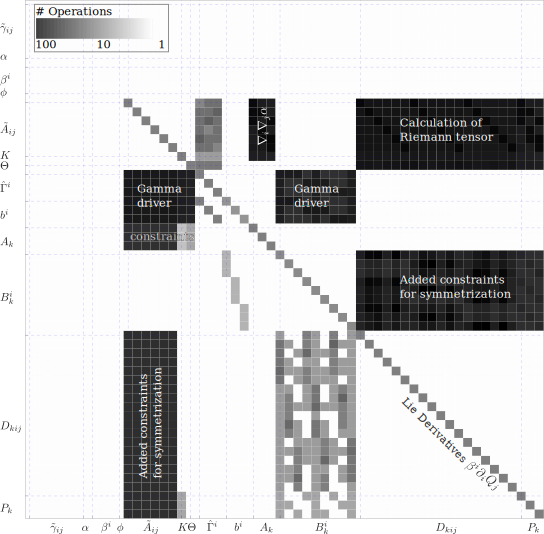
\includegraphics[width=\textwidth]{foccz4-cas/CCZ4-SystemMatrix-costs.pdf}
   	\caption[
     	FO-CCZ4 System matrix, evaluation costs (Mathematica sketch) \exclusive
   	]{
   		System matrix $\boldsymbol{A} \cdot \boldsymbol{n}$ with in
   		radial direction $\boldsymbol n = (1,1,1)$ as in
   		Figure~\protect\ref{fig:foccz4-sparsity}. Here, the color (shading) encodes the 
   		number
   		of basic operations
   		(additions and multiplications due to tensor contractions)
   		neccessary to compute the non-conservative product of that matrix element
   		on a logarithmic scale. The major blocks are labeled.
   		
   		The figure shows the two major cost drivers: The complex computation
   		of the Riemann (Ricci) tensor via the derivatives of the Christoffel
   		symbols via $D_{kij}$ (upper right) as well as the symmetrization
   		contributions which almost double the computational cost of the NCP.
   	}%
   	\label{fig:fo-ccz4-system-costs}
\end{figure}
%\todo[color=red]{Improve CCZ4 system cost image \ref{fig:fo-ccz4-system-costs}. It is really bad in the current shape.}

The \emph{costs} of a PDE system should measure its requirements in
runtime, memory and storage when being evaluated in a computer. Certainly,
in terms of memory requirements, due to the larger state vector, the costs
of the FO-CCZ4 system (59 unknowns) are certainly higher then of the SO-CCZ4
system (34 unknowns), which again is much more demanding then the original
ADM system (12 unknowns). When evaluated within the presented ADER-DG
scheme, the cost of the FO system will again be higher than the cost of
the SO system. This is due to the distinction between non-conservative product
(NCP) and source terms is made and the evaluation of the NCP takes place
several times within a timestep during the evaluation of the Riemann solver at
the cell boundaries. However, the FO system can also be evaluated with
traditional methods---Finite Differences and Runge Kutta (FDRK) where there
is only the right hand side differential operator.

The determination of
absolute costs is almost always inconclusive. For instance, the system
matrix, being a $\mathbb R^{n\times n}$ matrix, obviously grows with
$\mathcal O(n^2)$, where $n$ is the state vector size. A naive attemp is to
relate the cost ratio of FO/SO system to $58^2 / 34^2 \sim 2.9$. However,
this obviously does not even take the evaluation of tensors into account.
Figure~\ref{fig:foccz4-sparsity} already shows that the FO-CCZ4 system matrix
is sparse, and Figure~\ref{fig:fo-ccz4-system-costs} quantifies the differences
in terms of neccessary contractions to determine a certain element $A_{ij}$.
The amount of calculations varies over five orders of magnitude.
In other words, a few elements contribute to the overall number of
$\sim40,200$ elementary arithmetic operations (counting
special functions like $n^x$ and $x^n$ as one operation).
%\todo{FIGURE matrix \ref{fig:fo-ccz4-system-costs} needs adoption -- wie?}

\begin{margintable}[-6cm]
	\begin{tabular}{lcrr}
		\toprule
		Conf. & C & \#OP & $t$ [sec] \\
		\midrule
		\multirow{2}{*}{Dense}  & G & 8884 & 3.49 \\
		& I & 17761 & 8.92 \\
		\multirow{2}{*}{Sparse} & G & 5638 & 2.61  \\
		& I & 2757 & 6.14 \\
		\multirow{2}{*}{FullSimplify} & G & 4737 & 2.26  \\
		& I & 2730 & 4.42  \\
		\multirow{2}{*}{Optimized}  & G   & 5886 & 2.52  \\
		& I & 2821 & 5.77  \\
		\multirow{2}{*}{orderOpt} & G & 4141 & 2.76 \\
		& I & 1480 & 3.47 \\
		
		\bottomrule
	\end{tabular}
	\caption[
	Performance results of generating an optimized Z4 implementation
	]{
		\footnotesize % Fixme: "Table x.x" is in wrong fontsize
		Measuring the impact of differently ``optimized'' generated code
		to compute the NCP of the Z4 system. The first column describes
		the experiment, the second column shows which compiler was used
		to compile the Fortran code to assembler (G=GNU compiler,
		I=Intel compiler), \#OP indicates the number of assembler
		instructions which were generated while $t$ shows the serial
		runtime for $6\cdot10^6$ evaluations of the NCP with arbitrary
		but same state vectors (pseudo-randomly generated with the same seed).
		\\
		Experiments and interpretation are given in the main text.
	}\label{table:ccz4-implementation-optimization-minibenchmark}
\end{margintable}
%
A completely different measure is the number of assembler instructions
which have to be processed in order to compute a PDE function.
Table~\ref{table:ccz4-implementation-optimization-minibenchmark} provides
a small benchmark where different Fortran codes were generated by a CAS
(\code{Mathematica} and \code{Matlab} were used). In the first setup, all matrix elements
were specified, even the zero ones (\emph{Dense}), while in a second step,
the zero matrix elements were trivially removed (\emph{Sparse}). In a
subsequent step, a typical CAS ``simplification'' step (\emph{FullSimplify}) 
was performed, where algebraic expressions are brought in a form which requires
less evaluations (for instance by reducing polynomial expressions). The
\emph{Optimized} step further tried to store intermediate expressions to
variables, avoiding the need of computing certain expressions over and over
(trading memory for less arithmetic instructions). The \emph{orderedOpt} step
adopts a topological ordering of the required intermediate computations of the NCP
(adopting a task based paradigm), which should also reduce cache misses.

The results of this benchmarks are given as follows: While the number of
operations in principle can be decreased by one order of magnitude
(17kOP for the dense matrix vs. 1.4kOP for the topological ordered and
intermediate expressions computing version), the overall runtime stays in the
same regime and sophisticated algebraic transformations of the computation
order do not pay off.

The reasons for this are that optimizing for a small
number of assembler instructions is not the right measure at a CISC platform
\footnote{Complex instruction set computers (CISC) have machine instructions
  for various high level functions, which however can vary largely in execution
  time. In contrast, the presented measure is considerably more meaningful for
  reduced instruction set computers (RISC). In the current HPC landscape, CISC
  machines dominate, while there is however a trend for more RISC machines.},
while sophisticated vectorization units of the machine were
not used at all\footnote{
  The lack of vectorization in CAS-generated code stems from the fact that the tensorial algebra was not
  expound to the CAS in the chosen approach. While tensorial packages for CAS
  are in principle available (\cf Section~\vref{sec:symbolic-computing}),
  the freely available C/Fortran code generators from both Mathematica™ and
  Matlab™ do not generate optimized tensor contraction loops, such as discused in 
  Section~\ref{sec:implementing-ccz4-language}.
}. Therefore, a static analysis of code runtime is not meaningful.

%Furthermore, a benchmark run at a single core has little significance on
%a realistic multi core environment (\ie within an AMR code) where the full
%use of a compute node effects completely different memory and processor
%availability.


\subsection{Choosing the right language}\label{sec:implementing-ccz4-language}
There are several aspects that emerge when implementing large tensorial PDE systems.
First, as in physics, where the suitable choice of a coordinate system
can greatly reduce the complexity of a problem, or in mathematics, where
the transformation of a problem to another theory can provide new insights
and shortcuts, a suitable notation of the PDE system in a
computer-readable language/form reduces the abstraction neccessary from physics and
the equations as they are written on the paper.

The smallest common
demoninator in modern scientific programming languages is that of
\emph{linear algebra}, providing a compact language to manipulate
$n$-dimensional arrays in one expression (instead of looping over
vector or matrix axes). However, linear algebra misses a number of
features from differential geometry, for instance the distinction from
covariant and contravariant tensors. There is in fact the need for
a \emph{domain specific language} (DSL) which implements a minimum on
tensor algebra, \ie general style contractions (applying Einstein
sum convention).

As an example, an exemplaric contraction which shall compute $D^i$ is 
given,
\begin{equation}\label{eq:tensoralgebra-example}
D^i := A^{ik} B^{nm} C_{knm}
\end{equation}
with arbitary tensors $A,B,C$, where not even symmetries such as
$B^{nm} = B^{mn}$ shall be relevant at this point. While the mathematical
expression \eqref{eq:tensoralgebra-example} provides a clear instruction
how $D^i$ is defined by sums, thanks to associativity of addition and
multiplication, several evaluation strategies may lead to $D^i$. For
the FO-CCZ4 equations, using the \code{TensorTemplates} package
allows to write down this expression precisely as
\begin{equation}
\vec D = \TT{contract}{1,0}
 \left( A, \TT{trace}{0,2}\left(
   \TT{contract}{0,2}(B,C) \right) \right)
\end{equation}
This notation is declarative in a sense that it does not expose how
a contraction or trace is computed internally\footnote{
  The technical advantage (which comes on top of readability) of
  this abstraction is the fact that the implementation of the
  operation can be done efficiently by the compiler, for instance
  by exploting parallelization in terms of SIMD-vectorization.
} and it reveals the intermediate evaluation sequence as
\begin{equation}
A^{ik} B^{nm} C_{knm} \to A^{ik} E_{mkn} \to A^{ik} E_k \to D^i
\,.
\end{equation}
Providing efficient tensor algebra as a library is a whole branch of HPC
itself, and there is a plentitude of librarys available, however only a subset
of them deals with covariance\footnote{other covariance-aware tensor
libraries are for instance
the \code{Deal.II Library} \cite{Alzetta2018,Bangerth2007},
the \code{Tensor Contraction Engine} 
\cite{Baumgartner2005,Lam2011,Baumgartner2003},
\code{BARRACUDA} \cite{Nelson2015}, \code{InTensLi} \cite{Li2015}}.

\section{Benchmarks for solving FO-CCZ4 with ADER-DG}
%
\label{sec.tests}

In the following we present a battery of standard tests that explore the
ability of our formulation to carry out long-term stable evolutions of a
number of different spacetimes with increasing degree of curvature. If
not stated otherwise, in all of the tests we set initially $\Theta = 0$,
$\hat{\Gamma}^i = \tilde{\Gamma}^i$ and $b^i = 0$ and the HLLEM method is
used (Section~\ref{sec:holy-dg-scheme}).

In all tests the algebraic constraints on the
unit determinant of $\tilde{\gamma}_{ij}$, the zero trace of
$\tilde{A}_{ij}$ as well as the constraint $\tilde{\gamma}^{ij} D_{kij} =
0$ (which is a consequence of $|\tilde{\gamma}_{ij}|=1$) have all been
\textit{rigorously enforced} in the discrete solution
$\u_h(\boldsymbol{x},t^n)$ at the beginning of each timestep, but they
have \textit{not} been enforced during the computation of the spacetime
predictor $\q_h$. Note that the predictor $\q_h$ is only an auxiliary
quantity that is overwritten after each timestep and which has a role
similar to the evolution stage to the half timelevel in second-order 
MUSCL-Hancock type TVD finite-volume schemes.
%Note that in the very common case of a semidiscrete scheme evolved in
%time with a high-order Runge-Kutta (RK) time integrator, our choice
%corresponds to enforcing the constraints after a full timestep, but not
%in all the intermediate RK stages.
We therefore set $\tau \to \infty$ and thus neglect the corresponding
source terms. In tests involving black holes, the lower limit on the
lapse is set to be $\ln(\alpha) \geq -20$. We will use the notation $P_N$
to indicate an ADER-DG scheme using piecewise polynomials of degree $N$
to represent $\u_h$.

\subsection{Linearized gravitational-wave test}
%
\begin{marginfigure}
     \includegraphics[width=\textwidth]{foccz4-paper-official/LinearWave-P5-04-ADM.pdf}
        
     \includegraphics[width=\textwidth]{foccz4-paper-official/LinearWave-P5-04-waveform.pdf}
     \includegraphics[width=\textwidth]{foccz4-paper-official/LinearWave-P9-02-ADM.pdf}
     \includegraphics[width=\textwidth]{foccz4-paper-official/LinearWave-P9-02-waveform.pdf}
     \caption[
       Linearized GW test, 1D cuts and time series \ownPub{Dumbser2017}
     ]{Linearized gravitational-wave test using an ADER-DG $P_5$
      scheme with 4 elements (panels 1-2) and an ADER-DG $P_9$ scheme with
      only 2 elements (panels 3-4). The temporal evolution of the
      constraints (colour panels) is shown together with the waveform for
      the component $\tilde{A}_{22}$ of the traceless conformal extrinsic
      curvature after 1000 crossing times at time $t=1000$.}
    \label{fig.linearwave}
\end{marginfigure}
%
The first test problem is a simple one-dimensional wave-propagation test
problem in the linearized regime. The computational setup follows the one
suggested by in \cite{Alcubierre:2003pc}. The
computational domain is $\Omega = [-0.5,0.5]$ with periodic boundary
conditions in the $x$ direction and two simulations are run until a final
time of $t=1000$: \textit{(i)} a first one using 4 ADER-DG $P_5$ elements
(\ie a total number of 24 degrees of freedom) and \textit{(ii)} a second
one using only 2 ADER-DG $P_9$ elements (\ie only 20 degrees of
freedom). This test is run with the unlimited version of the ADER-DG
scheme. The exact solution of the metric of the problem is given by
%
\begin{align}
\label{eqn.lw.metric}
\d s^2 &= - \d t^2 + \d x^2 + (1+h) \d y^2 + (1-h) \d z^2\,, \\
\textnormal{with} \quad
h &:= \epsilon \sin \left( 2 \pi (x-t) \right)\,,
%
\end{align}
%
and the wave amplitude $\epsilon = 10^{-8}$ is chosen small enough in
order to stay in the linear regime, so that terms
$\mathcal{O}(\epsilon^2)$ can be neglected. Since the shift is zero in
the metric \eqref{eqn.lw.metric} ($\beta^i = 0$), we set $s=0$ in our
FO-CCZ4 system and furthermore harmonic slicing is used, \ie
$g(\alpha)=1$. We also set $K_0=0$, $c=0$, $e=2$ and use the 
\textit{undamped} version of the system, setting $\kappa_1 = \kappa_2 =
\kappa_3 = \eta = 0$. 
%We note that when setting $s=0$ and adopting a harmonic slicing it is
%necessary to choose $e > 1$ in order to get a strongly hyperbolic system,
%hence we use $e=2$. 
Using the metric \eqref{eqn.lw.metric}, the 
definition of the extrinsic curvature reduces to $K_{ij} = -
\tfrac{1}{2}\partial_t \gamma_{ij}/(\alpha)$, so that the various
components are given by $K_{xx} = K_{xy} = K_{xz} = K_{yz} = 0$, $K_{yy}
= -\halb \partial_t h$ and $K_{zz} = +\halb \partial_t h$. From this
information, the conformal factor $\phi$, the conformal spatial metric
$\tilde{\gamma}_{ij}$, the traceless conformal extrinsic curvature
$\tilde{A}_{ij}$ and all auxiliary variables can be computed by a direct
calculation according to their definitions.

In Fig. \ref{fig.linearwave} we report the temporal evolution of all ADM
constraints (Hamiltonian and momentum constraints) as well as the errors
of the algebraic constraints on the determinant of the conformal metric
and the error in the trace of $\tilde{A}_{ij}$ in both cases, \ie using
the ADER-DG $P_5$ and $P_9$ scheme. A comparison of the
extrinsic-curvature component $\tilde{A}_{22}$ with the exact solution is
also provided at the final time $t=1000$, showing overall an excellent
agreement between numerical and exact solution. The quality of the
results obtained with the ADER-DG schemes used in this paper, which are
uniformly high-order accurate in both space and time, is significantly
superior to the results shown in \cite{Alcubierre:2003pc} for the
same test problem using a finite difference scheme with much more grid
points (between 50 and 200) compared to the very coarse mesh containing
only 20 to 24 degrees of freedom used in our simulations. Note that a
fair comparison between high order finite-difference and DG schemes must
be made in terms of points per wavelength for finite-difference methods
and in degrees of freedom per wavelength for DG schemes.


\subsection{Gauge-wave test}
%
\begin{marginfigure}
	\includegraphics[width=\textwidth]{foccz4-paper-official/GaugeWaveA01-Waveform-phi.pdf}
	\includegraphics[width=\textwidth]{foccz4-paper-official/GaugeWaveA01-Waveform-K.pdf}

    \caption[
      Gauge-wave test, linear regime \ownPub{Dumbser2017}
    ]{Gauge-wave test case with amplitude $A=0.1$ using the
      undamped FO-CCZ4 system ($\kappa_1=\kappa_2=\kappa_3=0$) and
      improved cleaning speed $e=2$ with no damping $c=0$.
      Comparison with exact solution after $t=1000$.}
    \label{fig.gaugewave}
\end{marginfigure}
%
\begin{marginfigure}
    \includegraphics[width=\textwidth]{foccz4-paper-official/GaugeWaveA09-Waveform-phi.pdf}
    \includegraphics[width=\textwidth]{foccz4-paper-official/GaugeWaveA09-Waveform-K.pdf}
    \caption[
      Gauge-wave test, nonlinear regime \ownPub{Dumbser2017}
    ]{Highly nonlinear gauge-wave test case with very large
      amplitude $A=0.9$. Comparison of the wave form with the exact
      solution at time $t=10$ for an ADER-DG $P_5$ scheme and $100 \times
      10$ elements.}\label{fig.gauge.xxl}
\end{marginfigure}
%
Also this classical test problem has been taken from the collection of
standard tests of \cite{Alcubierre:2003pc}. The metric in this case
is given by
%
\begin{equation}
\begin{aligned}
\label{eqn.gw.metric}
\d s^2 &= - H(x,t) d t^2 + H(x,t) \d x^2 + \d y^2 + \d z^2\,, \\
\textnormal{with} \quad H(x,t) &:= 1-A\,\sin \left( 2\pi(x-t)
\right)\,.
\end{aligned}
\end{equation}
%
The metric \eqref{eqn.gw.metric} implies zero shift ($\beta^i = 0$),
hence we use once more $s=0$ together with harmonic slicing
$g(\alpha)=1$. Also for this test we employ the \textit{undamped} version
of the FO-CCZ4 system, setting $\kappa_1 = \kappa_2 = \kappa_3 = \eta =
0$. The computational domain in this case is two-dimensional, with $\Omega = [-0.5,0.5] \times
[-0.05, 0.05]$ with periodic boundary conditions in all directions. Since
$\beta^i = 0$, the extrinsic curvature is again given by $K_{ij} =
-\partial_t \gamma_{ij} / (2\alpha)$, \ie $K_{yy} = K_{zz} = K_{xy} =
K_{xz} = K_{yz} = 0$ and the remaining primary variables are
%
\begin{equation*}
\phi^2 = H^{-1/3}, \qquad  \alpha = \sqrt{H}, \qquad
K_{xx} = - \pi A\frac{\cos\left(2\pi(x-t)\right)}{\sqrt{1 - A\sin\left(2\pi(x-t)\right)}}.
\end{equation*}
We furthermore set $K_0=0$. The auxiliary variables can be
obtained from their definition via a straightforward calculation.

We first simulate this test problem with a perturbation amplitude of
$A=0.1$ until $t=1000$ with an unlimited ADER-DG $P_3$ scheme and using
$100 \times 10$ elements to cover the domain $\Omega$. We run this
physical setup twice, once with the default parameters $e=c=1$, according
to the original second order CCZ4 system \cite{Alic:2011a} and a
\textit{modified} setting with $e=2$ and $c=0$ to obtain an improved
cleaning of the Hamiltonian constraint. In both cases the system is
strongly hyperbolic.  The time evolution of the ADM constraints is
reported in Fig. \ref{fig.gaugewave}, showing only a very moderate growth
of the constraint $M_2$ that is sublinear in time and close to machine
precision. The other constraints $H$ and $M_1$ remain essentially
constant during the entire simulation.  We emphasize that we have used
the \textit{undamped} version of the FO-CCZ4 system, and nevertheless
obtain stable results, while the original second-order CCZ4 formulation
was reported to fail for this test problem in the undamped version, and
only the damped CCZ4 system was stable (see \cite{Alic:2011a} for
details). It is also worth recalling that both the first- and the
second-order formulation of the BSSNOK system fail for this test case
after a rather short time \cite{Alic:2011a, Brown2012}. In
Fig. \ref{fig.gaugewave} we also provide a direct comparison of the
solution after 1000 crossing times for the conformal factor $\phi$ as
well as for the trace of the extrinsic curvature $K$.
Note the overall 
very good agreement between the numerical solution and the exact
one. For the sake of clarity, in the plots of the waveforms we also
report the numerical error computed as the difference between the 
numerical solution and the exact solution at the final time $t=1000$. 
It can be clearly noticed from the computational results shown in Fig. 
\ref{fig.gaugewave} that the constraints and the phase errors in the 
waveforms are significantly smaller for the 
modified setting $e=2$, which may justify the use of a faster cleaning 
speed of the Hamiltonian constraint $e>1$ for \textit{purely numerical} 
purposes. In any case, our FO-CCZ4 system behaves well also with the 
default setting $e=c=1$, which is typically used in the standard 
second order CCZ4 system \cite{Alic:2011a}.

Since the gauge-wave test has a smooth nontrivial exact analytical
solution and is also valid in the nonlinear regime of the equations, we
can use it in order to perform a numerical convergence study. For this
purpose, we run the test again with different unlimited ADER-DG $P_N$
schemes on a sequence of successively refined meshes. To make the test
more difficult, we choose a very large perturbation amplitude of $A=0.9$,
which takes the system in the highly nonlinear regime, although in the
end the test consists only in a nonlinear re-parametrization of the flat
Minkowski spacetime. For thise case we use $c=0$ and $e=2$. We set the 
final simulation time to $t=10$ and continue using the \textit{undamped} 
version of the FO-CCZ4 system. 

\begin{table}[t]
	\caption[
	Gauge Wave convergence table \ownPub{Dumbser2017}
	]{Numerical convergence results for the large amplitude gauge wave
		test problem with $A=0.9$ at a final time of $t=10$.  The $L_2$
		errors and corresponding observed convergence order are reported for
		the variables $\phi$, $\alpha$ and $K$.
		Here, $\mathcal O({x})$ means the convergence order for $x$.
	}
	\centering\begin{adjustbox}{center,scale=0.9}
		%\renewcommand{\arraystretch}{1.0}
		\begin{tabular}{ccccccc}
			\hline
			$N_x \times N_y$ & ${L_2}$ error $\phi$ & $\mathcal{O}(\phi)$  & ${L_2}$ error $\alpha$ & $\mathcal{O}(\alpha)$  & ${L_2}$ error $K$ & $\mathcal{O}(K)$  \\
			\hline
			\multicolumn{7}{c}{$N=3$}   \\
			\hline
			$60 \times  6$  & 2.8663E-05 &     & 5.4876E-05 &      & 3.8469E-03 &      \\
			$80 \times  8$  & 1.0574E-05 & 3.5 & 2.2314E-05 & 3.1  & 7.0357E-04 & 5.9  \\
			$100\times 10$  & 3.8760E-06 & 4.5 & 8.0170E-06 & 4.6  & 2.3112E-04 & 5.0  \\
			$120\times 12$  & 1.6311E-06 & 4.7 & 3.2521E-06 & 4.9  & 9.7392E-05 & 4.7  \\
			\hline
			\multicolumn{7}{c}{$N=4$}   \\
			\hline
			$60 \times  6$  & 4.2966E-06 &     & 1.1408E-05 &      & 2.1910E-04 &      \\
			$80 \times  8$  & 8.9473E-07 & 5.5 & 2.3725E-06 & 5.5  & 5.0194E-05 & 5.1  \\
			$100\times 10$  & 2.5596E-07 & 5.6 & 6.8053E-07 & 5.6  & 1.5781E-05 & 5.2  \\
			$120\times 12$  & 9.0039E-08 & 5.7 & 2.4064E-07 & 5.7  & 6.1004E-06 & 5.2  \\
			\hline
			\multicolumn{7}{c}{$N=5$}   \\
			\hline
			$40 \times  4$  & 8.9305E-07 &     & 2.1971E-06 &      & 1.3614E-04 &      \\
			$60 \times  6$  & 5.2103E-08 & 7.0 & 1.2756E-07 & 7.0  & 5.9568E-06 & 7.7  \\
			$80 \times  8$  & 7.1947E-09 & 6.9 & 1.7348E-08 & 6.9  & 8.4259E-07 & 6.8  \\
			$100\times 10$  & 1.5357E-09 & 6.9 & 3.6421E-09 & 7.0  & 1.8093E-07 & 6.9  \\
			\hline
			\multicolumn{7}{c}{$N=7$}   \\
			\hline
			$30 \times 3$  & 1.7693E-08 &      & 3.9004E-08 &       & 6.3103E-06 &       \\
			$40 \times 4$  & 1.8387E-09 & 7.9  & 4.1751E-09 &  7.8  & 5.5791E-07 &  8.4  \\
			$60 \times 6$  & 6.2824E-11 & 8.3  & 1.4304E-10 &  8.3  & 2.1519E-08 &  8.0  \\
			$80 \times 8$  & 5.6521E-12 & 8.4  & 1.3455E-11 &  8.2  & 1.7085E-09 &  8.8  \\
			\hline
		\end{tabular}
	\end{adjustbox}
	\label{tab.conv1}
\end{table}

\begin{marginfigure}[-6cm]
	\includegraphics[width=\textwidth]{foccz4-paper-official/GaugeWaveE1-Constraints.pdf}
	\includegraphics[width=\textwidth]{foccz4-paper-official/GaugeWaveA01-Constraints.pdf}
	\caption[
	GaugeWave: Constraint evolution \ownPub{Dumbser2017}
	]{Growing of constraint violations during the Gauge Wave evolution.
		Note the logarithmic scale.}
	\label{fig.gaugewave2}
\end{marginfigure}

The $L_2$ error norms of the conformal factor $\phi$, the lapse $\alpha$ and
the trace of the extrinsic curvature $K$, together with the observed
order of accuracy of the different ADER-DG schemes are reported in Table
\ref{tab.conv1}. We observe essentially the expected order of accuracy of
the scheme for $N=3$ and $N=4$, while a superconvergence is observed for
$N=5$ and $N=7$. We think that this is due to the strong nonlinearities
of the PDE system appearing in the regime in which we run this test case
with $A=0.9$ and that some leading errors may be dominated by quadratic
terms in the metric and the conformal factor, which can lead to a faster
error decay than $N+1$ for \textit{coarse} meshes. However, we expect
that this superconvergence will disappear on sufficiently refined meshes;
but since the absolute errors are already getting close to machine
accuracy on the meshes used here, it is not possible to refine the mesh
much more with double-precision arithmetics, at least in the $N=7$ case.
For the ADER-DG $P_5$ scheme using $100 \times 10$ elements a comparison
between numerical and exact solution of the nonlinear waveforms for
$\phi$, $\alpha$, $K$ and $D_{xxx}$ is provided in Fig.
\ref{fig.gauge.xxl} at $t=10$, where we can note again an excellent
agreement between exact and numerical solution.

\subsection{Robust stability test}
%
\begin{marginfigure}
	\includegraphics[width=\textwidth]{foccz4-paper-official/RobustStabilityODE-10x10.pdf}
	\includegraphics[width=\textwidth]{foccz4-paper-official/RobustStabilityODE-80x80.pdf}
	\caption[
	Robust scability test \ownPub{Dumbser2017}
	]{Robust stability test case with Gamma-driver shift condition
		and $1+\log$ slicing with random initial perturbation of amplitude
		$10^{-7}/\rho^2$ in all quantities on a sequence of successively
		refined meshes on the unit square in 2D using an ADER-DG $P_3$
		scheme. Upper: $10\times10$ elements, corresponding to $40\times40$
		degrees of freedom ($\rho=1$). Lower: $80\times80$ elements, corresponding
		to $320\times320$ degrees of freedom ($\rho=8$). }
	\label{fig.robstab}
\end{marginfigure}
%
The  robust stability test is the last standard test problem
that we take from Ref. \cite{Alcubierre:2003pc}. While in the previous
test problems we have used a simple frozen shift condition $\partial_t
\beta^i = 0$ by setting $s=0$ in the FO-CCZ4 system, here we employ the
classical Gamma-driver shift condition. Furthermore, we employ the
$1+\log$ slicing condition, setting the slicing function to
$g(\alpha)=2/\alpha$ and the parameter $f$ of the Gamma driver to
$f=0.75$, which is also the typical value used for the BSSNOK system and
for the classical second-order CCZ4 system \cite{Alic:2011a}.
We further set $e=2$, $\kappa_1=\kappa_2=\kappa_3=0$, $K_0=0$,
$c=1$ and $\eta=0$.

As customary in this test, we start from the flat Minkowski metric.
We then add uniformly distributed \textit{random perturbations} to
\textit{all} quantities of the FO-CCZ4 system, \ie to all primary and
auxiliary variables and also to $\Theta$ and $\hat{\Gamma}^i$.  The
two-dimensional computational domain is $\Omega = [-0.5,0.5]^2$ and we
run different simulations with an unlimited ADER-DG $P_3$ scheme on four
successively refined meshes composed of $10 \rho \times 10 \rho$
elements, corresponding to $40 \rho \times 40 \rho$ degrees of freedom,
where $\rho \in \left\{ 1, 2, 4, 8 \right\}$ is the refinement factor.
The perturbation amplitude is $\epsilon = 10^{-7}/\rho^2$, which
corresponds to perturbation amplitudes that are three orders of magnitude
larger that those suggested in \cite{Alcubierre:2003pc}.

The time evolution of the ADM constraints is reported in Fig.
\ref{fig.robstab} for all four simulations. One can observe that after an
initial decay the constraints remain essentially constant in time for all
different grid resolutions, indicating that our FO-CCZ4 system indeed
passes the robust stability test with the standard Gamma driver and
$1+\log$ gauge conditions (see \cite{Cao:2012} for similar tests with the
Z4c system).



\subsection{Convergence tests on three-dimensional black-hole spacetimes}
\label{sec:convergence-bh3d}

In this test we consider the evolution of isolated Schwarzschild and Kerr
black holes in 3D Cartesian Kerr-Schild coordinates, with $M=1$ the mass
of the black hole and $a$ the dimensionless spin. The metric in these
coordinates is known analytically and thus the primary variables of our
evolution system are given by
%
\begin{equation}
  \alpha = S^{-\halb}\,, \qquad
	\beta^i = \frac{2 H}{S} l_i\,, \qquad
	\gamma_{ij} = \left( \begin{array}{ccc}
	 1 + 2 H l_x^2 & 2 H l_x l_y & 2 H l_x l_z \\
	 2 H l_x l_y & 1 + 2 H l_y^2  & 2 H l_y l_z \\
	 2 H l_x l_z & 2 H l_y l_z & 1 + 2 H l_z^2
	\end{array} \right)\,,
	\label{eqn.kerr.metric}
\end{equation}
%
with
%
\begin{equation*}
	 H := M \frac{r^3}{r^4 + a^2 z^2}\,, \qquad
	 S := 1 + 2 H\,, \qquad
	 l_x := \frac{r x + a y}{r^2 + a^2}\,, \qquad
	 l_y := \frac{r y - a x}{r^2 + a^2}\,, \qquad
	 l_z := \frac{z}{r}\,,
\end{equation*}
%
and
%
\begin{equation*}
r := \sqrt{ (x^2 + y^2 + z^2 - a^2)/2 + \sqrt{((x^2 + y^2 + z^2 -
    a^2)/2)^2 + z^2 a^2} }\,.
\end{equation*}
%
We furthermore use the fact that the solution is stationary, \ie
$\partial_t \gamma_{ij}=0$, hence the extrinsic curvature $K_{ij}$ is
computed as follows \cite{Rezzolla_book:2013}
%
\begin{equation}
K_{ij} = \frac{1}{2\alpha} \left( \nabla_i \beta_j + \nabla_j \beta_i
\right)\,.
\end{equation}
%

\begin{table*}[b]
	\caption[
	   Convergence results for different BH coordinates, 
	\ownPub{Dumbser2017}
	]{Numerical convergence results of FO-CCZ4 with simplified Gamma
		driver for the Schwarzschild black hole (left) and the Kerr black
		hole (right) in 3D Cartesian Kerr-Schild coordinates at a final time
		of $t=10$.  The $L_2$ errors and corresponding observed convergence
		order are reported for the variables $\phi$.}
	\label{tab.conv.bh}
	\vspace{.5cm}%
	\renewcommand{\arraystretch}{1.0}
	\begin{tabular}{cccccccccccc}
		\hline
		\multicolumn{6}{c}{\textbf{Schwarzschild black hole} ($a=0$)}   & \multicolumn{6}{c}{\textbf{Kerr black hole} ($a=0.9$)}   \\
		\hline
		$N_x$ & ${L_2}$ error $\phi$ & $\mathcal{O}(\phi)$  & $N_x$ & ${L_2}$ error $\phi$ & $\mathcal{O}(\phi)$  &
		$N_x$ & ${L_2}$ error $\phi$ & $\mathcal{O}(\phi)$  & $N_x$ & ${L_2}$ error $\phi$ & $\mathcal{O}(\phi)$  \\
		\hline
		\multicolumn{3}{c}{$N=3$}  &  \multicolumn{3}{c}{$N=5$}    &
		\multicolumn{3}{c}{$N=3$}  &  \multicolumn{3}{c}{$N=5$}    \\
		\hline
		10	& 9.9982E-06	&     &   5 & 2.1837E-06 &     & 10	& 1.4270E-05	&     &   5 & 2.6679E-06 &     \\
		15	& 1.8439E-06	& 4.2	&  10 & 2.8327E-08 & 6.3 & 15	& 2.8279E-06	& 4.0 &  10 & 6.5136E-08 & 5.4    \\
		20	& 5.8521E-07	& 4.0	&  15 & 2.3649E-09 & 6.1 & 20	& 8.9487E-07	& 4.0 &  15 & 6.0944E-09 & 5.8    \\
		25	& 2.4322E-07	& 3.9	&  20 & 4.1176E-10 & 6.1 & 25	& 3.6468E-07	& 4.0 &  20 & 1.1087E-09 & 5.9    \\
		\hline
	\end{tabular}
\end{table*}
%
The function $K_0$ is chosen as $K_0 = \left( K - \beta^k \partial_k
\alpha \right)/{\left(\alpha^2 g(\alpha)\right)}$, so that $ \partial_t
\alpha = 0$ and in this test the Gamma-driver shift condition is
simplified to $\partial_t \beta^i = f b^i$, $\partial_t B_k^i = f
\partial_k b^i$ and $\partial_t b^i = \partial_t \hat{\Gamma}^i$, with
the consequence that the above exact solution corresponds to a stationary
solution of the FO-CCZ4 system. In other words, we remove the advection
terms from the evolution equations of the shift $\beta^i$ and the
variable $b^i$ (see also \cite{Alcubierre:2008}). The conformal factor
$\phi$ and the auxiliary variables can be computed according to their
definition. The computational domain is chosen as $\Omega = [1,5]^3 \,
M^3$, and the exact solution given by the initial condition is imposed on
all boundaries in all variables at all times. Note that this choice of
boundary conditions is appropriate to study convergence since the exact
solution is also a stationary solution of our PDE system. Note also that
the black hole is centered at $x=y=z=0$, so that we evolve only a section
of the domain offset from the singularity, but encompassing regions both
inside and outside of the event horizon; this effectively amounts to
employing an excision of the black-hole interior.  We furthermore set
$e=2$, $c=1$, $\eta=0$, and consider the undamped CCZ4 system with the
$1+\log$ slicing, \ie we set $\kappa_1 = \kappa_2 = \kappa_3 = 0$,
$f=0.75$ and $g(\alpha)=2 / \alpha$.

The simulations were performed with different ADER-DG schemes on a
sequence of successively refined meshes until a final time of
$t=10\,M$. The Rusanov method is used as approximate Riemann solver at
the element interfaces. In the case of the Schwarzschild black hole we
use $a=0$, while for the Kerr black hole we set $a=0.9$. The
corresponding numerical convergence rates are reported for both cases in
Table \ref{tab.conv.bh}, where we observe that the designed order of
accuracy $N+1$ of our high-order fully-discrete one-step ADER-DG schemes
has been properly reached.


\subsection{Evolution of a single puncture black hole}
\label{sec.single.punctures}

We next have applied the FO-CCZ4 formulation to a single puncture black
hole \cite{Brandt97b} with mass $M=1$ and dimensionless spin $a=0$
located at the origin of a three-dimensional computational domain $\Omega
= [-150,150]^3 \, M^3$ with periodic boundary conditions on all
boundaries. The
domain is discretized with an AMR mesh with grid spacing $\Delta x =
\Delta y = \Delta z = 2.5\,M$ within the inner box $\Omega_b = [-15,15]^3
\, M^3$, while $\Delta x = \Delta y = \Delta z = 7.5\,M$ is used in the
outer part of the domain. In the innermost zone $\Omega_l = [-3,3]^3 \,
M^3$ the third-order subcell ADER-WENO finite-volume limiter is activated
throughout the entire simulation. For details on the AMR framework and
the subcell finite-volume limiter we refer the interested reader again to
\cite{Dumbser2014,Zanotti2015c,Zanotti2015b}. We also stress that this
simulation can be run only after activating the finite-volume subcell
limiter, since a robust scheme is needed in order to deal with the
puncture singularity. Without such a limiter, \ie with a pure DG scheme,
the code crashes after a few timesteps since the high-order unlimited DG
scheme is \textit{not} robust enough to deal with the puncture metric. In
our simulation we use an ADER-DG $P_3$ scheme ($N=3$), which leads to
$2N+1 = 7$ finite-volume subcells per DG element, \ie the effective mesh
spacing in terms of points (cell averages) inside the domain $\Omega_l$
is $\Delta x = \Delta y = \Delta z = 0.357\,M$.  Note that we set up the
mesh so that the puncture is located at the boundary of the DG elements;
given the location of the degrees of freedom in the subcell grid, no grid 
point coincides with the puncture.
We set the CCZ4 parameters to $\kappa_1 = 0.1$, $\kappa_2=0$, $\kappa_3 =
0.5$ and $\eta=0$. The constant $\mu$ accounting for the second-order
ordering constraints in the evolution of $B^i_k$ is set to $\mu=1/5$,
while for this test we use $c=1$, $f=0.75$ and $e=1$ to be as close as 
possible to a standard second-order CCZ4 formulation, where the cleaning 
of the Hamiltonian constraint is done at the speed of light.

\begin{marginfigure}
	\includegraphics[width=\textwidth]{foccz4-paper-official/SinglePunctureBH-ODE-eta0.pdf}
	\includegraphics[width=\textwidth]{foccz4-paper-amended/OnePunctureODE-zoom.png}
	\caption[
	Single puncture black hole, constraint evolution \ownPub{Dumbser2017}
	]{Time evolution of the ADM constraints for the single
		puncture black hole using an ADER-DG $P_3$ scheme with AMR and
		ADER-WENO subcell finite-volume limiter until $t=1000$ (left). Color
		contours for the lapse at $t=200$ and grid setup showing the domain
		$\Omega$, the refined box $\Omega_b$ and the zone with active subcell
		finite-volume limiter $\Omega_l$ (center). Zoom into the center
		region at $t=200$ with color contours for $\alpha$ (right).}
	\label{fig.puncture}
\end{marginfigure}

% 
The initial metric and lapse are provided by the \texttt{TwoPunctures}
initial data code \cite{Ansorg:2004ds} (part of the \code{Einstein Toolkit}
 \cite{loeffler_2011_et}). Explicitly, the lapse is set initially
to
\begin{equation}
    \alpha = \halb \left(\frac{1-\halb \left({M}/{r^*}\right)}{1+\halb
        \left({M}/{r^*}\right)}+1\right)\,,
\end{equation}
%
where $r^*:=(r^4+10^{-24})^{\frac{1}{4}}$ and $r$ is the coordinate
distance of a grid point from the puncture. The auxiliary quantities
(which are spatial derivatives of the primary quantities) are obtained
via a simple fourth order central finite difference applied to the
primary variables $\alpha$ and $\gamma_{ij}$. Initially the shift and the
extrinsic curvature are set to zero, \ie $\beta^i = 0$ and $K_{ij}=0$.

The evolution was carried out until a final time of $t=1000\,M$ and
Fig. \ref{fig.puncture} reports the evolution of the average $L_2$ error
of the ADM constraints, which we define as
%
\begin{equation*}
\overline{L}_2 = \sqrt{ \frac{\int_\Omega \epsilon^2
    \d\boldsymbol{x}}{\int_\Omega d\boldsymbol{x} } }\,,
\end{equation*}
%
where $\epsilon$ denotes the local error of each of the ADM quantities,
\ie Hamiltonian $H$ and momentum constraints $M_i$. In Fig. \ref{fig.puncture}
also a view of the 3D grid setup is shown together with a zoom into the center 
region with the contour colors of the lapse function at a time of $t=200\,M$.  
%
It is probably worth recalling that, to the best of our knowledge, these
are the first results obtained for a puncture black-hole spacetime using
a fully three-dimensional DG finite-element method with AMR and LTS.
Previous results obtained with high-order DG schemes for black-hole
spacetimes were essentially limited to the one-dimensional case 
\cite{field10, Brown2012, Miller2016}.

\newpage
\subsection{Preliminary results for moving punctures}\label{sec.movpunct}
\begin{marginfigure}
	\includegraphics[width=\textwidth]{foccz4-paper-official/TPRusanov-t00.pdf} 
	\\[.3em]
	\includegraphics[width=\textwidth]{foccz4-paper-official/TPRusanov-t07.pdf}
	\\[.3em]
	\includegraphics[width=\textwidth]{foccz4-paper-official/TPRusanov-t10.pdf}
	\\[.3em]
	\includegraphics[width=\textwidth]{foccz4-paper-official/TPRusanov-t15.pdf}
	\caption[
	  BH-BH head-on collision, time evolution snapshots, \ownPub{Dumbser2017}
	]{Time evolution of the contour surfaces of the lapse $\alpha$
		and the shift vector $\beta^i$ for the head-on collision of two
		puncture black holes of equal mass $M=1$ at times
		$t=0,\,5,\,7,\,8,\,10\,M$ and $t=15\,M$, from top left to bottom
		right.}
	\label{fig.twopunctures}
\end{marginfigure}

The last test considered is a preliminary application of the FO-CCZ4
system to a binary system of two moving punctures. In particular, we
consider a head-on collision of two nonrotating black holes of equal mass
$M=1$ with zero linear momentum initially located at $\boldsymbol{x}^- =
(-1,0,0)$ and $\boldsymbol{x}^+ = (+1,0,0)$. The three-dimensional
computational domain is given by $\Omega = [-25,25]^3 \, M^3$ and flat
Minkowski spacetime is imposed as boundary condition everywhere.  The
CCZ4 parameters are set to $\kappa_1 = 0.1$, $\kappa_2=0$, $\kappa_3 =
0.5$, $\eta=0$ and furthermore we choose $c=1$, $e=1$, $f=1$ and $\mu=1/5$.
Again, the initial metric and the lapse are provided by the
\texttt{TwoPunctures} initial data code \cite{Ansorg:2004ds}, with the lapse
set initially to
\begin{equation}
    \alpha =
    \halb\left(
    \frac{1-\halb\left({m_-}/{r_-^*}\right)-\halb\left({m_+}/{r_+^*}\right)}
    {1+\halb\left({m_-}/{r_-^*}\right)+\halb\left({m_+}/{r_+^*}\right)}
    +1  \right)\,,
\end{equation}
where $r^*_-$ and $r^*_+$ are the coordinate distances of a grid point
from either puncture (defined analogously to the previous section) and
$m_-$ and $m_+$ are the  bare masses of the two black holes (see
\cite{Ansorg:2004ds}) and in this case they are equal. The auxiliary
quantities are computed from the primary variables via a fourth-order
central finite-difference method. We use the simple and robust Rusanov
method as approximate Riemann solver on the element boundaries.  The
shift and extrinsic curvature are initially set to $\beta^i = 0$ and
$K_{ij}=0$.

The domain is discretized with an AMR mesh of mesh spacing $\Delta x =
\Delta y = \Delta z = 5/12\,M$ within the inner box $\Omega_b =
       [-2.5,2.5]^3 \, M^3$, while $\Delta x = \Delta y = \Delta z =
       1.25\,M$ is used in the outer part of the domain. In the innermost
       zone $\Omega_l = [-5/3,5/3]^3 \, M^3$ the third-order subcell
       ADER-WENO finite-volume limiter is activated throughout the entire
       simulation. As for a single puncture, we use an ADER-DG $P_3$
       scheme ($N=3$), whose $2N+1 = 7$ finite-volume subcells lead to an
       effective mesh spacing inside the domain $\Omega_l$ of $\Delta x =
       \Delta y = \Delta z = 0.0595$. Once again we remark that the use
       of the finite-volume subcell limiter is essential in order to
       obtain a stable evolution.

The simulation is run until a final time of $t=60\,M$ and the evolution
of the contour surfaces of the lapse and the shift vector are reported in
Fig. \ref{fig.twopunctures}. The contour surfaces of the conformal factor
at the final time as well as the evolution of the ADM constraints are
depicted in Fig. \ref{fig.twopunctures.adm}. Clearly, no sign of growth
in the violation of the constraints appears after the two punctures have
merged at $t\simeq 10\,M$.

Although these results are meant mostly as a proof-of-concept rather than
as a realistic modelling of the inspiral and merger on binary black-hole
systems, they provide convincing evidence that binary systems of puncture
black holes can be evolved stably with our path-conservative ADER-DG
scheme with ADER-WENO subcell finite-volume limiter on AMR grids based on
the FO-CCZ4 formulation proposed here. A more detailed and systematic
investigation, which includes the emission of gravitational waves from
binary systems of rotating black holes in quasi-circular orbits 
\cite{Alic:2011a}, will be the subject of future work.

\section{Summary}
\begin{marginfigure}
	\includegraphics[width=\textwidth]{foccz4-paper-official/TPRusanov-phi-t34.pdf}
	\includegraphics[width=\textwidth]{foccz4-paper-official/TPCollisionADM.pdf}
	\caption[
	BH Head-on collision, final snapshot and error time evolution, 
	\ownPub{Dumbser2017}
	]{Head-on collision of two puncture black holes: contour
		surfaces of the conformal factor $\phi$ at time $t=34\,M$ after the
		merger (left) and time evolution of the ADM constraints (right).
		The curves for the second and third momentum constraint almost
		coincide. }
	\label{fig.twopunctures.adm}
\end{marginfigure}

In Chapter~\ref{chapter:gr}, the evolution from classical 3+1 formulation of
Einsteins field equations over BSSNOK and the Z4 family to CCZ4 was passed. The
rewriting of CCZ4 to a first order formulation was discussed in detail and
remarks on mathematical and computer-science (implementation) related points
were made. Afterwards, the ADER-DG scheme from Section~\ref{sec:dg} was applied
in order to demonstrate the correctness of the PDE and applicability of the
scheme in a couple of standard numerical relativity testbeds. Some of these
tests are especially remarkable, since these are the first simulations of 
black-hole spacetimes ever performed in three spatial dimensions with high-order
discontinous galerkin methods. However, all examples shown in this sections
were restricted to ``vacuum solutions'' of Einsteins equations, where the
matter contribution $T_{\mu\nu}$ is exactly zero. Chapter~\vref{chapter:hydro}
is dedicated to discuss the powerful and widespread theory of hydrodynamics 
for a non-zero assignment of $T_{\mu\nu}$ in the given equations, while 
providing its standalone evolution equations for individual quantities
resembling the energy momentum tensor.



\subtitledChapter{ADER-DG schemes for the general-relativistic magnetohydrodynamic equations}
   {Hydrodynamics}\label{chapter:hydro}
% Definitions from exahype-advanced-hydro.tex
% in math mode: Description before symbol
\newcommand{\desc}[1]{\text{#1}\quad} % -> shall inline
% abbrevations in math mode
\newcommand{\hydro}{\text{HD}}
\newcommand{\mhd}{\text{MHD}}
\newcommand{\adm}{\text{ADM}}
\newcommand{\hd}{\text{HD}}
\newcommand{\srhd}{\text{SRHD}}
\newcommand{\grhd}{\text{GRHD}}
\newcommand{\grmhd}{\text{GRMHD}}
\newcommand{\bmag}{\text{B}}
\newcommand{\magneto}{\text{MD}} % magnetodynamics

% left aligned vectors (pmatrix is center aligned)
\newenvironment{pvector}{\begin{pmatrix*}[l]}{\end{pmatrix*}}

This chapter summarizes efforts of solving the equations of general relativistic
magnetohydrodynamics (GRMHD) with the finite-volume limited ADER-DG scheme
introduced in Chapter~\vref{chapter:numerics}. 
An introduction into the problem and a review of previous work given in
Section~\vref{sec:hd-intro}. This chapter is prepended a motivation abou
the physical modeling of neutron stars spacetimes.
The subsequent Chapter~\vref{chapter:bnslt}
will demonstrate an actual application (beyond academic benchmark scenarios).
This chapter relies partially on the publications \cite{Fambri2018,Koeppel2017}.

\section[
  Motivation: An effective theory for dense and hot matter
]{Motivation: An effective theory for dense and hot nuclear 
matter}\label{sec:hd-nuclear-matter}
The most compact astrophysical object after a black hole is a neutron star.
Having roughly the mass of the sun, the star radius is only at the kilometer
scale, thus only an order of magnitude larger then its Schwarzschild radius.
\footnote{To provide some numbers, the solar mass $\Msol \approx 2 \times 
10^{30}$~kg complies with its Schwarzschild radius $R_\sol \approx 3$~km.
n contrast, typical neutron stars with $M \approx 2 \Msol$
have a radius at the order of $R\approx 10$~km.}. 
Astrophysically, these objects are interesting as the endpoint of a supernovae.
Pulsars, being neutron stars (or white dwarfs) emitting characteristic
highly intensive beams of electromagnetic radiation, are amongst the most
fascinating and best studied compact objects in astronomy.

For an high energy physicist, neutron stars are interesting because they allow 
to probe all fundamental forces: Of course gravity, electromagnetism, but also
the weak and strong force. In
neutron stars, energy and density regimes can be reached which are out of
range for particle accelerators. An understanding of neutron star interiours
thus allows to falsify or set limits in nuclear and fundamental theories.
As an example, within the merger of a binary neutron star system, it is likely
that the quark phase transition can be probed.
\todo[color=green]{HD, Intro: Would nice to have references for QGP excursion.}

In order to describe the physics of a neutron star, the best fundamental
theories available are the standard model of particle physics, written in the
language of special-relativistic quantum field theory, and general relativity,
the (non-quantum) theory of gravity \footnote{In fact, a neutron star does not 
even come close to take backreactions of quantum matter onto the spacetime into
account, and therefore quantum corrections are not required in Einstein field
equations (in contrast as in section~\ref{sec:motivation-qbh}).}.

The typical approach to solve the \emph{spacetime} of a single isolated
neutron star requires taking in an averaged, thermalized
energy-momentum tensor at a given spatial position. This motivates to find a
suitable effective theory (or phenomenological model) for the matter dynamics
which is thermodynamically motivated, leaving the (fundamental) particle
physics picture behind \footnote{Section~\vref{sec:tov} will go into detail of
an ideal fluid model of a neutron star, the TOV solution.}. The physical branch
of fluid mechanics provides a suitable theory, which is (relativistic)
hydrodynamics. 
% It subsumes all physics on micro scales within an \emph{equation
%of state}.

\section{Introduction of Hydrodynamics}
Hydrodynamics adopts two features: Coarse graining, \ie the averaged 
thermodynamic description
of a system, and fast thermalization, \ie the fact that the fluid is locally
assumed to be in a well-defined thermodynamic equilibrium state
\footnote{
 For it's power of describing effective phenomenae, hydrodynamics is sometimes
 called an ``effective theory of everything''.
}.
\emph{Ideal} hydrodynamics is based on the \emph{perfect fluid hypothesis}: 
Dynamical timescales are much larger then viscous or heat transfer timescales. 
Furthermore, the fluid is assumed to be isentropic, \ie there are no prefered 
direction effects. This allows to assume stresses to be isotropic. Furthermore,
there is no heat transport and viscosity and no dissipation. Beyond the ideal
theory, there are (more) realistic theories of hydrodynamics which add
particular features, such Navier-Stokes equations, the classical theory of
viscous fluids \footnote{In this thesis, only ideal fluids are covered, while
 references to extensions are given at some points.}.

The \emph{dynamical timescale} of a gravitational systems is given by
\cite{Rezzolla_book:2013}
\begin{equation}
\tau_\text{dyn} \sim 1/\sqrt{G\bar\rho} \,,
\end{equation}
with an average rest mass density $\bar \rho$ and here the explicit Newton's
constant~$G$. The dynamical time scale of nuclear
matter (nuclear density $\rho_\text{nuc} \approx 2.3\times 10^{17}$kg/m$^3$)
is $\tau_\text{dyn} \sim 2 \times 10^{-4}\text{s}$.
%$\sim 200\mu\text{s} \sim 40 \Msol$.
In comparison, the viscous and heat timescales
are typically of the order of 10$^{+8}$s and therefore can be ignored.
\todo[color=green]{HD Intro: Find reference for viscous/heat timescales}

The relativistic perfect ideal fluid is described by the stress energy tensor
\begin{equation}
T_{\mu\nu} = \rho h u_\mu u_\nu + p g_{\mu\nu}\,,
\end{equation}
with rest mass density $\rho$, 4-velocity $u_\mu=\d{x^\mu}/\d{\tau}$ 
(which is timelike, $u^\mu u_\mu=-1$) and specific internal energy
$\epsilon$ as part of the specific enthalpy $h=1+\epsilon+p/\rho$. The
pressure $p$ subsumes all physics on micro scales within an
\emph{equation of state} $p=p(\rho,\epsilon)$.
The relativistic total energy density is $e=\rho(1+\epsilon)$ and
$g_{\mu\nu}$ is the usual 4-metric.

Widespread simple equations of state are the one-parametric ideal-fluid
(or ``Gamma-law'') equation of state $p=\rho\epsilon(\Gamma-1)$
with the adiabatic / polytropic index $\Gamma$, and the polytropic
EOS $p=\kappa \rho^\Gamma$.

Hydrodynamics can be derived from a number of different fundamental principles,
for instance the principle of minimal action \cite{Andersson2007}
or from kinetic theoryby applying a moment scheme to the Boltzmann equations
\cite{Rezzolla_book:2013}. While a derivation is out of the scope of this
text, the equations of motion as well as the resulting PDEs are discussed
in the subsequent sections. The fluid dynamics are dictated by two conservation
equations for the 4-energy momentum tensor $T^{\mu\nu}$ and for the rest mass
(density flux) $\rho u^\mu$, \ie
\begin{equation}
T^{\mu\nu}=0, \quad \nabla_\mu (\rho  u^\mu) = 0\,.
\end{equation}

Instead of deriving the actual PDEs, the different parts of the 
flux-conser\-vative formulation of general realtivistic magnetohydrodynamics
(GRMHD)  shall be discussed in the next sections \footnote{
  Naturally, such a discussion can either be ordered \emph{top-down}, \ie
  starting from the advanced theory and advancing into the low-energy limit,
  or \emph{bottom-up}, \ie starting with the classical, easy theory and
  advancing by proposing additions neccessary to fulfill relativity, curved
  background and to incorporate Maxwell's theory. Both approaches are well 
  known in theoretical physics. In this text, I decided for
  the \emph{bottom-up} strategy.
}. The state vector of GRMHD,
%\footnote{
%	Remind that the ordering of state vectors has no physical meaning
%	(Section~\ref{sec:conservation-laws}).
%}
\begin{equation}
Q_\grmhd = (Q_\hd, Q_\adm, Q_\magneto) \,,
\end{equation}
is a composite of state vectors which origin from three different theories:
The state vector of hydrodynamics $Q_\hd$ (discussed in this section), 
the curved background metric, collected in the parameter $Q_\adm$ 
(discussed in Section~\ref{sec:grhd}) and the state vector of
magnetodynamics $Q_\magneto$ (Section~\ref{sec:grmhd}). The seperation of
theories by fundamental building blocks is also sketched in Figure
\ref{fig:composite-SVEC} and implemented in the \code{SVEC} GRMHD code.

\subsection{Classical Hydrodynamics}\label{sec:hydro-definitions}
% Some texts come from my Exahype-Engine/ApplicationExamples/GRMHD/doc
\begin{marginfigure}
	\begin{tikzpicture}[node distance=1cm]
	\node (Vhd) {$V_{hydro}$};
	\node[right=0.2cm of Vhd] (maxwell) {$Q_{B}$};
	\node[right=0.7cm of maxwell] (adm) {$Q_{ADM}$};
	
	\node[below of=Vhd] (Qhd) {$Q_{hydro}$}
	edge[<-] (Vhd.south);
	
	\node[below of=Qhd] (mhd) {$Q_{MHD}$}
	edge[<-] (Qhd.south)
	edge[<-] (maxwell.south);
	
	\node[below left of=mhd] (dens) {Densitied $Q_{MHD}$}
	edge[<-] (mhd.south);
	
	\node[below right of=dens] (grmhd) {GRMHD State vector}
	edge[<-] (adm.south)
	edge[<-] (dens.south);
	\end{tikzpicture}
	\caption[
	GRMHD State vector composition, Cartoon (tikZ), \exclusive
	]{State vector composition in GRMHD, or in particular, in
		the \code{SVEC} code.}%
	\label{fig:composite-SVEC}
\end{marginfigure}

%
Hydrodynamics can be introduced by defining the \emph{primitive} and 
\emph{conserved} state vector, where the later is evolved in time and the
former is required for the system closure, given by the pressure/equation of
state. The vectors are given as
\begin{alignat}{4}
\label{eq.hd.prim}
&\begin{array}{l}\text{Primitive}\\\text{vector}\end{array}
&
\quad u &=
\begin{pvector}
\text{rest mass density} \\
\text{velocity} \\
\text{internal energy}
\end{pvector}
= \begin{pmatrix} \rho \\ v_i \\ \epsilon \end{pmatrix}\,,
\\
\label{eq.hd.cons}
&
\begin{array}{l}\text{Conserved}\\\text{vector}\end{array}
&
Q_\hydro
&=
\begin{pvector}
\text{Conserved density} \\
\text{Momentum} \\
\text{Energy density}
\end{pvector}
=
\begin{pmatrix} D \\ S_j \\ E \end{pmatrix}\,,
\\
&
\begin{array}{l}\text{related by}%\\\text{Prim2Cons}
	\end{array}
%\desc{related by Prim2Cons}
~~
&
Q_\hd(u)
&=
\begin{pvector}
\rho \\
\rho v_j \\
\rho/2 v^2 + \epsilon
\end{pvector}\footnotemark\,.
\label{eq.hd.Qu}
\\
\intertext{
Classical hydrodynamics can be expressed in flux-conservative form 
\eqref{intro:conservation-law},
}
	\label{eq.hd.fluxes}
	&\text{with fluxes}
	& F^i_\hydro(u) &=
	\begin{pmatrix}
		\text{fluxes for } D \\
		\text{fluxes for } S_j \\
		\text{fluxes for } E
	\end{pmatrix}
	=
	\begin{pvector}
		\rho v^i \\
		W^i_j \\
		v^i (E + p)
	\end{pvector}
	\,.
\end{alignat}
\footnotetext{Note how easily the primitives $u(Q)=(\rho, S_j/\rho, 
E-\rho/(2v^2))$
	can be analytically recovered from the conserved variables (in contrast to
	relativistic hydrodynamics, presented in the next section). Therefore,
	the fluxes in equation \eqref{eq.grhd.fluxes} are also an algebraic 
	function of
	the conserved state vector only.
}%
The other PDE terms in \eqref{intro:conservation-law} are vanishing.
%
Here, we used the hydrodynamic energy-momentum-tensor (EM tensor), given by
\footnote{
	The EM tensor is also refered to as $W^{ij}=S^{ij}$ in the literature
	(and in Section~\ref{sec.3p1-emtensor}).}%
\begin{equation}\label{eq.hd.emtensor}
W^{ij} = S^i v^j + p \, \delta^{ij}  \, . \,\,
\end{equation}%
%
Classical hydrodynamics is a nonlinear theory. Within the \code{ExaHyPE} code,
it is widely used for performance measurements. Deriving the strong 
hyperbolicity of classical hydrodynamics is part of many books
\cite{Toro09,Rezzolla_book:2013}. The eigenvalues $\lambda_i$ in $k$-direction
in $d$ dimensions are then found to be
\begin{equation}\label{eq.hd.evs}
\lambda_1 = v_k - c,
\quad \lambda_{2,\dots,d+1} = v_k,
\quad \lambda_{d+2} = v_k + c \,,
\end{equation}
where $c=\sqrt{\left(\partial_\rho p\right)_s}$ is the \emph{sound speed} of 
the fluid. The three different wave speeds stand out as different waves in the
Riemann problem (Section~\ref{sec:riemann-problem}).

\subsection{Special relativistic hydrodynamics (SRHD)}
Special relativistic hydrodynamics is the extension of classical
hydrodynamics valid for high velocities ($v\to c$), but remaining on flat
background spacetime.

The 3-velocity $v^i$ of the fluid is extended in favour of the
Lagrangian 4-velocity $u^\mu = (W,W v^\mu)$, with Lorentz factor $W=(1- 
v^2)^{-1/2}$
\footnote{
	In the literature, alternative popular namings are $W=\Gamma$, $E=U$.
	In any case, do not confuse $W$ with the conformal factor used in
	some conformal formulations of Einstein Equations (see Section~\ref{sec:conformal-factor}).
}.
The 4-momentum/rest-mass current is then given by $S^\mu = \rho u^\mu$.
The content of the primitive \eqref{eq.hd.prim} and conserved vector
\eqref{eq.hd.cons} does not change. However, the relationship \eqref{eq.hd.Qu}
is replaced by
\begin{equation}
	Q_\srhd(u)
	=
	\begin{pvector}
	\rho W \\
	\rho h W^2 v_j \\
	\rho h W^2 - p - \rho W
	\end{pvector}
	\label{eq.srhd.Qu}
\end{equation}
with specific enthalpy $h=1+\epsilon+p/\rho$
\footnote{Some groups prefer to evolve $Q_\srhd=(D,S_j,\tau)$ instead
	of $Q_\srhd=(D,S_j,E)$ with $\tau=E-D$ the rescaled energy density.
	In fact we will also stick to this convention.
}.
The conservative formulation of SRHD is then given by is then given by the 
fluxes
\begin{align}
	\label{eq.srhd.fluxes}
	F^i_\hydro(u) &=
	\begin{pmatrix}
		\text{fluxes for } D \\
		\text{fluxes for } S_j \\
		\text{fluxes for } \tau
	\end{pmatrix}
	=
	\begin{pvector}
		D v^i \\
		W^i_j \\
		S^i - v^i D
	\end{pvector}
	\,.
\end{align}
The SRHD equations are hyperbolic for causal EOS \cite{Anile_book,Font08}. The
wave speeds decompose similarly as in \eqref{eq.hd.evs}, where however the
relationship to the speed of sound $c$ is nonlinear \cite{Font08},
\begin{equation}
\lambda_\pm
=
\frac{v^k (1-c^2) \pm c \sqrt{(1-v^2)(1-v^2c^2 - v_k^2 (1-c^2))}}{1-v^2 c^2}
\end{equation}
and $\lambda_- := \lambda_1, \lambda_+ := \lambda_{d+2}$ in the notation of
\eqref{eq.hd.evs}.

% Note that if you add terms
%to the energy-momentum tensor (such as the magnetic terms), also $S_j$
%will change (c.f. \eqref{eq.grhd.Qu} to XXX).

\subsection{The primitive recovery in relativistic hydrodynamics}\label{sec:c2p}
Due to the nonlinear Lorentz factor $W=W(v^2)$, the recovery of the primitive
variables \eqref{eq.hd.prim} from the conserved ones \eqref{eq.hd.cons} is no 
more possible analytically in SRHD. Instead, the inverse of \eqref{eq.srhd.Qu}
can be approximated by numerical root finding. The standard approach is to
solve a single or multiple nonlinear equations. For instance, the authors of
\cite{DelZanna2007,Noble2006} propose to solve a simple nonlinear $2 \times 2$
system which reads for SRHD as
\begin{equation}
\begin{rcases}
  y^2 x - S^2 &= 0 \\
  y - p - E   &= 0 
\end{rcases}\,,
\end{equation}
with $x=v^2, y=\rho h W^2$. Once
$x$ and $y$ are determined numerically, all primitives can be recovered by
computing $W=(1-x)^{-1/2}$, $\rho=D/W$, $v_j=S_j/y$,
$h=S_j/(v_j\rho W^2)$ and for instance with the ideal gas (from above), 
$\epsilon=h/(1+W)$\footnote{Obviously any non-analytic EOS raises new issues at
	this point which are again subject to numerical treatment.}.


\section{General relativistic hydrodynamics (GRHD)}\label{sec:grhd}
General relativistic hydrodynamics is the theory which described fluids moving
within an (external) gravitational potential. The (special) relativistic fluid
follows the definitions from the previous section. The coupling of the
background spacetime is mediated by a source term in the law of motion.

A fully general relativistic description implies also matter backreaction on
the spacetime (the fluid bends spacetime itself), according to Einstein's field
equations (EFE, Chapter~\ref{chapter:gr}). In this case, the EFE determine the
dynamics of the geravitational field under the presence of a source term
(the energy momentum tensor of the fluid). Section \ref{sec:Cowling-approx}
discusses the simplifications which can be made to the GRMHD equations
when the backreaction is neglected.

\subsection{3+1 split of special relativistic hydrodynamics}
The ``Valencia formulation'' of GRHD presented in this thesis dates back to the
pioneering work of Mart\'i et al. \cite{Marti91, Banyuls97, Ibanez01} in 1991.
They where the first to make a characteristic approach to relativistic
hydrodynamics in a 3+1 split of spacetime \footnote{
see Section~\vref{sec:adm-foliation} for the definitions of normal vector 
$n^\mu$, lapse $\alpha$, shift $\beta^i$ and 3-metric $\gamma_{ij}$.}.

In the 3+1 split,
the Lagrangian velocity $u^\mu$ can be casted as $u^\mu = W(n^\mu + v^\mu)$ and
the 3-velocity as $v^i  =  u^i/W + \beta^i/\alpha$. The 3+1 language also offers
beatiful interpretations, for instance is the projection of the fluid 4-velocity
on the purely spatial hypersurfaces just the Lorentz-decorated 3-velocity,
$\gamma^\mu_\nu u^\nu = W v^\mu$. Formally, the 3-energy-momentum-tensor can be
interpreted as extension from the flat case,
\begin{equation}\label{eq.wij.grhd}
W_{\hydro}^{ij} = W^{ij}_\srhd = S^i v^j + p \delta^{ij}
~\leftrightarrow~
W^{ij}_\grhd = S^i v^j + p \gamma^{ij}
\,.
\end{equation}
The SRHD fluxes are refined as
\begin{align}
\label{eq.grhd.fluxes}
F^i_\hydro(u) &=
\begin{pmatrix}
\text{fluxes for } D \\
\text{fluxes for } S_j \\
\text{fluxes for } \tau
\end{pmatrix}
=
\begin{pvector}
D w^i \\
\alpha W^i_j - \beta^i S_j \\
\alpha (S^i - v^i D) - \beta^i \tau
\end{pvector}
\quad
\text{(general $W^{ij}$)}
\\
&=
\begin{pvector}
D w^i \\
S_j w^i + p \delta^i_j \\
\tau w^i + p v^i
\end{pvector}
\hspace{2.7cm} % todo: push right
\text{(only $W^{ij}=S^i v^j + p\gamma^{ij}$)}
\label{eq.grhd.flux2}
\end{align}
It is convenient to write the fluxes with the vector
$w^i=\alpha v^i - \beta^i$ which is refered to as the advection
velocity relative to the coordinates, or just \emph{transport
	velocity}\footnote{Note that $w^i$ does not transform like a 3-vector. However,
	we introduce it only for abbreviation on the
    paper and for saving contractions in the computer.}. With the replacment
of $v^i \to w^i$, the GRHD fluxes \eqref{eq.grhd.flux2} have (almost) a similar
shape as the SRHD fluxes \eqref{eq.srhd.fluxes}.

In order to fully describe the state of a GRHD system, the local curvature must
be encoded in the state vector
\footnote{The ADM state is constant for the GRHD PDE, as the modification of the
	background spacetime is prescribed by Einstein field equations, which are 
	however
	a PDE on their own (Chapter~\ref{chapter:gr}). In \code{ExaHyPE} language, 
	an
	entry in the state vector which is not evolved by the PDE, \ie which 
	fulfills
	$\partial_t Q^k=0$, is called a ``material parameter''. This term comes from
	seismology where non-evolved parameters describe the immutable soil 
	properties
	(in GR lingua, the ``background'' spacetime) which are unchanged by the 
	waves
	described by the PDE.
}. Therefore, the ADM state vector is defined as
\begin{equation}\label{eq.grhd.adm}
Q_\adm = (\alpha, \beta^i, \gamma_{ij}, K_{ij}) \,.
\end{equation}
%
The GRHD system is hyperbolic \cite{Font00}, and the eigenvalues in $k$ direction
are given by
\begin{align}
 \lambda_0 &= \alpha v^k - \beta^k \,, \\
 \lambda_\pm &=
  \frac{\alpha}{1 - v^2 c_s^2}
  \big(  v^k (1-c_s^2) \nonumber\\
  &\phantom= \pm c_s
  \sqrt{(1-v^2)\left( \gamma^{kk}(1-v^2 c_s^2) - v^k v^k (1-c_s^2) \right)}
  \big) - \beta^k \,, 
\end{align}
with the local sound speed $c_s=\sqrt{\partial_\rho p + p/\rho^2 \partial_\epsilon p}/h$.

\subsection{Conformal factor}
In the Valencia formulation, the PDE system is written in terms
of tensor densities. The determinant of the metric
$\gamma=\text{det}(\gamma_{ij})$ relates the tensor densities with
an ordinary tensor. The 3-determinant is related to the determinant of
the four-metric by $\sqrt{-g}=\alpha\sqrt{\gamma}$. The system is
then formulated as\footnote{Here the full system \eqref{intro:ncp}
  is given, even if some terms are zero for certain systems
  (such as the algebraic and differential source for HD and SRHD).
}
\begin{equation}\label{eq:conformal-pde-grmhd}
\partial_t (\sqrt{\gamma} Q)
+ \partial_i (\sqrt{\gamma} F^i)
+ \sqrt{\gamma} B^i \partial_i (\sqrt{\gamma} Q)
= \sqrt{\gamma} S.
\end{equation}
The PDE as given in \eqref{eq:conformal-pde-grmhd} defines the
state $Q$, the fluxes $F^i$, the non-conserva\-tive part $B^i$ and the
algebraic source $S$ \emph{without} the factor $\sqrt{\gamma}$.
This convention will be retained for the following sections. Note that,
however, the vector $\sqrt \gamma Q$ is evolved in time.

\subsection{Sources for curved spacetimes}
In presence of a curved background, the spacetime coupling introduces
a source. The governing equations of GRHD are therefore a balance law
\eqref{intro:balance-law} instead of a conservation law
\eqref{intro:conservation-law}. The source term induced by the
spacetimes, written \emph{with Christoffel symbols}, read
\footnote{Note the use of 4-dimensional tensors except the lapse $\alpha$.
  See also Appendix~\ref{apx:symbols} for the standard definitions of
  the Christoffel symbols of first kind $\Gamma^k_{ij}$ and 4-metric
  $g_{\mu\nu}$.
}
\begin{equation}
S_\hydro(u) =
\begin{pvector}
\text{source for } D \\
\text{sources for } S_j \\
\text{source for } \tau
\end{pvector}
=
\begin{pvector}
0
\\
T^{\mu\nu} \partial_\mu g_{\nu j} - \Gamma^\delta_{\nu\rho} g_{\rho j} T^{\mu\nu}
\\
\alpha T^{\mu 0} \partial_\mu \ln \alpha - \alpha T^{\mu\nu} \Gamma^0_{\mu\nu}
\end{pvector}.
\end{equation}
In order to determine the 4-energy-momentum-tensor
\begin{equation}\label{eq.grhd.tmunu}
T^{\mu\nu} =
\rho h W^2 (n^\mu + v^\mu) (n^\nu + v^\nu)
   + p(\gamma^{\mu\nu} - n^\mu n^\nu)
\,,
\end{equation}
the 4-velocity $u^\mu$ or the normal vector $n^\mu$ have to be recovered.
This can be circumvented by using spatial tensors only: The equivalent
``Christoffel symbol free'' source terms, as used in \cite{Radice2013c},
read
\begin{equation}\label{eq:grmhd.source}
S_\hydro(u) =
\begin{pvector}
0
\\
\frac \alpha2 S^{lm} \partial_j \gamma_{lm} + S_k \partial_j \beta^k - E \partial_j \alpha
\\
\textcolor{red}{ \alpha S^{ij} K_{ij} } - S^i \partial_i \alpha
\end{pvector}
\,.
\end{equation}
The sources can also be written without computing the 
3-energy-momentum-tensor $S^{ij}$, exploiting
$\left(\partial_i \sqrt\gamma\right) / \sqrt\gamma = \frac 12 \gamma^{lm} 
\partial_i \gamma_{lm}$,
\footnote{
  However, \eqref{eq:grmhd.source2} requires to compute
  $\partial_i \sqrt \gamma$, which must then be (formally) part of the
  state vector if the non-conservative product approach is chosen.
}
\begin{equation}\label{eq:grmhd.source2}
S_\hydro(u) =
\begin{pvector}
0
\\
\frac \alpha2 S^l v^m \partial_j \gamma_{lm} + \alpha p \frac 1{\sqrt{\gamma}} 
\partial_j \sqrt{\gamma} + S_k \partial_j \beta^k - E \partial_j \alpha
\\
\textcolor{red}{
	\alpha S^l v^m K_{lm} - \alpha p \gamma^{lm} K_{lm}
} - S^i \partial_i \alpha
\end{pvector}
\end{equation}
All terms in the source except the red one(s) contain derivatives of the ADM
state vector \eqref{eq.grhd.adm}. This motivates to extend the definition of
the curvature state vector as
\begin{equation}\label{eq.grhd.admTilde}
\tilde Q_\adm = (
   \alpha, \beta^i, \gamma_{ij}, K_{ij},
   \partial_i \alpha, \partial_i \beta^j, \partial_i \gamma_{jk}
   ) \,.
\end{equation}
If \eqref{eq.grhd.admTilde} is chosen in favour of \eqref{eq.grhd.adm}, then
the GRHD source term is a purely algebraic one. In preparation of a coupled
evolution of GRHD with spacetime, either $Q_\adm$ or $\tilde Q_\adm$ must be
evolved in time. In fact, all quantities \eqref{eq.grhd.admTilde} are part of
the FO-CCZ4 state vector \eqref{eq:foccz4-state-vector}, proposed in
Section~\ref{sec:fo-ccz4}. Therefore, the GRHD part in a coupled evolution of
the presented GRHD system with the FO-CCZ4 formulation is of the form
\begin{equation}
\partial_t Q_\hd + \partial_i F^i_\hd(Q_\hd, \tilde Q_\adm)
 = S_\hd(Q_\hd, \tilde Q_\adm) \,.
\end{equation}
In contrast, an ordinary second order formulation of EFE would instead evolve
only $Q_\adm$ in time, \ie without the derivatives. In such a case, the 
differential
and algebraic split of the source term (Section~\ref{sec:ncp}) is applicable.
Part of the work carried out in \cite{Fambri2018} is to cast the PDE as
\eqref{intro:ncp}, \ie to cast all non-red summands as 
$B^{ij}_k(Q_\adm, Q_\grhd) \partial_i (Q_\adm)_j$.

In order to cast these PDEs into the algebraic-differential source
split \eqref{intro:ncp}, all black terms obtain an extra minus when they
are moved from the RHS to the LHS. The final GRHD system reads
then (colors now omitted):
\begin{align}
\left( B_\grhd \right)^{ij}_{k} \partial_i Q_j =%&=
\begin{pvector}
0
\\
- \frac \alpha2 S^{lm} \partial_j \gamma_{lm} - S_k \partial_j \beta^k + E \partial_j \alpha
\\
S^i \partial_i \alpha
\end{pvector} \,,
%\\
\quad
S_\grhd =%&=
\begin{pvector}
0
\\
0
\\
\alpha S^{ij} K_{ij}
\end{pvector} \,.
\end{align}

\subsection{Cowling approximation}\label{sec:Cowling-approx}
In case of a stationary spacetime (Cowling approximation
\cite{Cowling41}, characterized by $\partial_t g_{ij} = 0$),
one can simplify the source terms and
get rid of the contraction \citep{MTW1973, York79, Gourgoulhon2012}
\begin{equation}\label{eq:path-to-cowling}
S^{ij} K_{ij} = \frac{1}{2\alpha} S^{ik} \beta^j \partial_j
\gamma_{ik} + \frac 1\alpha S^j_i \partial_j\beta^i
\,.
\end{equation}
In this particular case, \eqref{eq:grmhd.source} simplifies to
\begin{equation}
S_{\hydro\text{,Cowling}}(u) =
\begin{pvector}
0
\\
\frac \alpha2 S^{lm} \partial_j \gamma_{lm} + S_k \partial_j \beta^k - E \partial_j \alpha
\\
\frac 12 S^{ik} \beta^j \partial_j \gamma_{ik} + S^j_i \partial_j \beta^i - S^i \partial_j \alpha
\end{pvector}
\,.
\label{eq.grmhd.cowling.source}
\end{equation}
In this special case, it is possible to write the GRHD equations without any
algebraic source term. All terms in \eqref{eq.grmhd.cowling.source} can
then be casted in the form $B\partial_i Q$. This allows to split the PDE as
\footnote{
  In the form \eqref{eq.grhd.as-cowling}, the flow on a background spacetime is 
  drescribed
  similiarly as in the shallow-water equations,
  where the bottom-slope term (which accounts for gravitational forces)
  can also be cast as a non-conservative product
  \cite{Pares2006,Castro2006,Castro2010}.  
}
\begin{equation}\label{eq.grhd.as-cowling}
\partial_t Q^k + \underbrace{\partial_i F^i(Q)}_\text{Hydro. contribution}
+ \underbrace{B^i_{jk} \partial_i Q_j}_\text{Background contribution}
= 0
\,.
\end{equation}
In the numerical schemes proposed in Section~\ref{sec:dg}, the absence of
an algebraic source is desirable, as it supports the well-balanced property
of these schemes.

\section{General relativistic magnetohydrodynamics (GRMHD)}\label{sec:grmhd}

The general relativistic magnetohydrodynamics (GRMHD) equations are
the consequence of the coupling of Euler equations 
(Hydrodynamics, GRHD) to Maxwell equations (Magnetodynamics, MD). In the
popular ideal MHD approximation, the electric field $\vec E = \vec B \times \vec v$
is fully determined by the moving fluid.
In this approximation, the Faraday tensor $F^{\mu\nu}$ (with 6 degrees of freedom,
$\vec E$  and $\vec B$) reduces to the magnetic field $\vec B$ only, therefore the
vector of conserved variables in Magnetodynamics is just $Q_\magneto = (B^i)$.
\footnote{We add further evolution equations in case of the divergence
   cleaning technique. However, note that there is no distinction between
   primitive and conserved variables in Magnetodynamics.}
This approximation is appropriate to describe a wide variety of astrophysical
phenomena where the electrical conductivity of the plasma (description
of matter) is very high. In the ideal MHD approximation, the electrical
conductivity $\sigma\to\infty$ is assumed to be divergent. The electrical field is
completely determined by the fluid velocity and the magnetic field.
The magnetic flux $\phi_B = B_i S^i$
over any surface $\boldsymbol S$ is conserved,
\begin{align}
\oint_{\partial \boldsymbol{S}} \left( \boldsymbol{E} +\boldsymbol{v}
\times \boldsymbol{B}\right) \cdot d\boldsymbol{\ell} = - \frac{d
	\phi_B}{d t} = 0\,,
\end{align}
and is advected with the fluid movement. The magnetic contribution to the
hydrodynamics equations, \ie the MHD equations, is then just a
conservation equation for the magnetic field.

\subsection{Magnetodynamics}
The photon field (Maxwell in vacuum, \ie without charge carriers) has the momentum
density $\boldsymbol S = \boldsymbol E \times \boldsymbol B$
(Poynting vector), total energy density $U = \frac{1}{2}\left(E^2 + B^2\right)$
and energy-momentum tensor $W^{jk}=U \gamma^{jk} - E^j E^k - B^j B^k$.

The electric field $\boldsymbol{E}$ in the Eulerian frame 
is determined by the simplified Ohm's law \ie $E_i = -
\tilde{\epsilon}_{ijk} v^j B^k$ in the ideal MHD limit
(\ie for diverging electrical conductivities).
The cross product is given by the spatial three-Levi-Civita tensor
density $\tilde{\epsilon}$ (see Appendix~\ref{apx:symbols} for the definition).
Therefore, the momentum density and energy momentum tensor can be expressed,
using only $\boldsymbol v$ and $\boldsymbol B$, as
\begin{align}
S^\magneto_i %= \left(\boldsymbol{E}\times\boldsymbol{B}\right)_i
&= \tilde{\epsilon}_{ijk} E^j B^k = -\tilde{\epsilon}_{ijk} \tilde{\epsilon}^{jmn} v_m B_n B^k
= v_i \left(B_k B^k \right) - B_i \left( v_k B^k\right)
\,,
\nonumber
\\
  W^{jk}_\magneto
   &=  U \gamma^{jk} - B^j B^k / W^2 - (B^k v_k) v^j B^k \,.
% = \boldsymbol{v} B^2 - \boldsymbol{B} \left(\boldsymbol{v}\cdot \boldsymbol{B}\right) .
\label{eq.md.contributions}
\end{align}

\subsection{The GRMHD coupling}
The Maxwell theory (Magnetodynamics) influence the hydrodynamic flow with the (energy)
momentum contributions \eqref{eq.md.contributions}, while the Euler theory
determines the electrical field in the presented ideal magnetodynamic approximation.
Furthermore, the pressure $p$ get's a magnetic contribution and is replaced in
\eqref{eq.wij.grhd} and \eqref{eq.grhd.tmunu} as
\begin{equation}
p \to p_\text{tot} = p_\hydro + p_\magneto
\quad\text{with}\quad
p_\magneto = \frac 12 \left( B_j B^j / W^2 + (B^j v_j)^2 \right)
\end{equation}
being the pressure contribution from ideal magnetodynamics.
The total energy-momentum tensor is the sum of all involved theories,
thus the GRM\-HD energy momentum tensor is given, for completeness, here as
\begin{equation}
\begin{aligned}
	W^{ij}_\grmhd &= W^{ij}_\hydro + W^{ij}_\magneto = W^{ij}_\hydro(p_\hydro + p_\magneto) + W^{ij}_\magneto
	\\
	&= 
	S^i v^j + p_\text{tot} \gamma^{ij} - \frac{B^i B^j}{W^2} - (B^k v_k)v^i B^j
	\,.
\end{aligned}
\end{equation}
Consequently, also the conserved quantities are given by
\begin{alignat}{3}
%	\desc{GRMHD P2C}
	&
	Q_\grmhd(u, Q_\magneto)
	&&=
	\begin{pvector}
		D \\
		S_j \\
		\tau
	\end{pvector}
	=
	\begin{pvector}
		\rho W \\
		D h W v_j + B^2 v_j - (B^i v_i) B_j \\
		D (h W -1) - p + \frac 12 \left( B^2 (1 + v^2) - (B^j v_j)^2 \right)
	\end{pvector}
	\label{eq.grhd.Qu}
\end{alignat}

\subsection{Fluxes and sources}
The evolution variables in GRMHD are
\todo[color=green]{MHD: Adress the issue that we
	evolve the \emph{covariant} momentum $S_j$ and the
	\emph{contravariant} magnetic field $B^j$. Why?}
\begin{equation}
Q_\mhd = (Q_\hydro, Q_\magneto) = (D, S_j, \tau, B^j)
\,.
\end{equation}
It should be emphasized that the vector of primitive variables \eqref{eq.hd.prim}
does not change (increase in size), the primitive recovery takes
only place for the hydrodynamic part of the GRMHD equations.
%
The MD conserved vector is just $Q_\magneto=(B^j)$ and its evolution is given
by the induction equation
\begin{equation}\label{eq.grmhd.pdeb.simple}
\partial_t B^j + \partial_i (w^i B^j - B^i w^j) = 0 \,,
\end{equation}
\ie the new PDE has fluxes and sources
\begin{equation}
F^i(Q) = w^i B^j - B^i w^j,
\quad S(Q) = 0 \,.
\end{equation}

The GRMHD equations are hyperpolic. For the characteristic wave speeds
in GRMHD, a popular choice is the magnetosonic approximation \cite{Gammie03}.
%
The evolution equation \eqref{eq.grmhd.pdeb.simple} does not handle the magnetic
field divergence, which is covered in the next section.

%
%\subsection{The pure GRMHD equations}
%In consequence, the simple tensor-free fluxes of GRHD as given in
%\eqref{eq.grhd.fluxes} are no more correct. Therefore, one typically
%employs the fluxes with the energy-momentum-tensor. We repeat the first
%three entries for the GRHD and give provide the new flux for the magnetic
%field in the pure GRMHD (\emph{without} divergence cleaning) as the 
%fourth entry:
%\begin{equation}
%F^i(u) =
%\begin{pmatrix}
%\text{fluxes for }D \\
%\text{fluxes for }S_j \\
%\text{fluxes for }D \\
%\text{fluxes for }B^j
%\end{pmatrix}
%=
%\begin{pmatrix}
%w^i D
%\\
%\alpha W^i_j - \beta^i S_j
%\\
%\alpha (S^i - v^i D) - \beta \tau
%\\
%\end{pmatrix}.
%\end{equation}
%The source terms for the magnetic fields $B^j$ are zero, similar to the
%source terms for the density $D$.
%
%This formulation is useful if one uses a technique to control the 
%Maxwell constraint $\partial_j B^j = 0$ which does not change the
%PDE system, for instance contraint transport.

\subsection[Divergence cleaning]{The divergence cleaning (constraint damping) 
formulation}\label{sec:divergence-cleaning}
The Maxwell magnetic monopole constraint $\partial_i B^i=0$ can be
casted as hyperbolic conservation law with a Generalized Lagrangian
Multiplier approach (GLM) also refered to as \emph{divergence cleaning},
initially proposed by \cite{Dedner:2002}. In this approach, the MHD
system is augmented with an additional auxiliary equation for an
artificial scalar field $\psi$ in order to propagate away numerical
violations of the divergence-free constraint\footnote{
  There are in fact other techniques to ensure in the divergence
  freedom of the magnetic field on a numerical level, such as
  constrained transport.
}.
\todo[color=green]{MHD: Tell more about constrained transport methods.}
Hence, the PDE \eqref{eq.grmhd.pdeb.simple} is replaced by two
different PDEs.
The MD conserved vector is now $Q_\magneto = (B^j, \phi)$. The
modified fluxes and sources read
\cite{Porth2017,Palenzuela:2008sf, Dionysopoulou:2012pp}
\begin{align}
	%\desc{fluxes}
	F^i(Q) &= \begin{pmatrix}
		\text{fluxes for }B^j \\
		\text{fluxes for }\phi
	\end{pmatrix}
	=
	\begin{pvector}
		w^i B^j - v^j B^i - B^i \beta^j \\
		\alpha B^i - \phi \beta^i
	\end{pvector}
	\\
	%\desc{and sources}
	S(Q) &=
	\begin{pmatrix}
		\text{sources for } B^j \\
		\text{sources for } \phi
	\end{pmatrix}
	=
	\begin{pvector}
		-B^i \partial_i \beta^j - \alpha \gamma^{ij} \partial_i \phi \\
		\textcolor{red}{- \alpha \kappa \phi} - \phi \partial_i \beta^i
		- \frac 12 \phi \gamma^{ij} \beta^k \partial_k \gamma_{ij}
		+ B^i \partial_i \alpha
	\end{pvector}
\end{align}
%
Here, $\kappa$ is the damping term which controls the amount of damping applied on the 
field $\phi$. In the sake of a sane balance law with purely differential 
source terms, $\kappa=0$ is a choice also carried out in \cite{Fambri2017}. This
choice reflects pure transport and no damping.

Notably, the divergence cleaning formulation introduces additional sourc\-es
which are mostly non-conservative (as in the case of GRHD) except of the
damping term (displayed in red). Thus, from all presented equations, only
a Cowling-GRMHD formulation with divergence cleaning and $\kappa=0$ has
zero algebraic sources.


\section{Benchmarks and GRMHD codes}
In the following sections, the solution of various academic benchmark
scenarios is demonstrated. These solutions have been obtained with the
path-conservative ADER-DG scheme presented in section \ref{sec:dg}.

%\subsection{The GRMHD PDE and its implementation}
In the \code{ExaHyPE} code, the full set of GRMHD equations
on dynamical spacetime with divergence
cleaning is implemented. The evolution quantities are given by
$Q_\grmhd=(D,S_j,\tau,B^i,\phi)$ and the PDE \eqref{intro:ncp} terms
are given by \footnote{
  The PDE presented in \cite{Fambri2018} completely avoids the
  algebraic source $S=0$, since all tests presented in the paper
  are carried out with stationary spacetime. Thus the hydrodynamic
  source term from Section~\ref{sec:Cowling-approx} is shown in
  \cite{Fambri2018}.
}
\begin{align}\label{eq.grmhd.summary}
	F^i(Q) &=
	\begin{pvector}
		\text{fluxes for } D \\
		\text{fluxes for } S_j \\
		\text{fluxes for } \tau \\
		\text{fluxes for }  B^j \\
		\text{fluxes for } \phi
	\end{pvector}
	=
	\begin{pvector}
		w^i D \\
		\alpha W^i_j - \beta^i S_j \\
		\alpha (S^i - v^i D) - \beta^i \tau \\
		w^i B^j - v^j B^i - B^i \beta^j \\
		\alpha B^i - \phi \beta^i
	\end{pvector}
	,
	\\
    B^{ij} \partial_i Q_j &=
	\begin{pvector}
	0
	\\
	- \frac \alpha2 S^{lm} \partial_j \gamma_{lm} - S_k \partial_j \beta^k + E \partial_j \alpha
	\\
	S^i \partial_i \alpha
	\\
	B^i \partial_i \beta^j + \alpha \gamma^{ij} \partial_i \phi \\
	\phi \partial_i \beta^i
	+ \frac 12 \phi \gamma^{ij} \beta^k \partial_k \gamma_{ij}
	- B^i \partial_i \alpha
	\end{pvector}
	,\,
	S =
	\begin{pvector}
	0
	\\
	0
	\\
	\alpha S^{ij} K_{ij}
	\\
	0
	\\
	- \alpha \kappa \phi
	\end{pvector}
	.
	\nonumber
\end{align}

The numerical code consists of three parts: The fundamental AMR code,
the numerical scheme which can solve a generic prototypic PDE
(see in general Chapter \ref{chapter:numerics}), and the particular PDE
parts, provided in \ref{eq.grmhd.summary}. Such an implementation requires
to perform a primitive recovery (Section \ref{sec:c2p}) at every evaluation
of $F^i$, $B^{ij}$ and $S$. 

\subsection{Benchmark description}
%\newcommand{\yes}{\Checkmark}
\newcommand{\yes}{\cmark}
\newcommand{\no}{\xmark}
\begin{table*}[t]
	\begin{tabularx}{\textwidth}{lXcccc}
		\toprule
		%        &      &                 &        & \multicolumn{2}{c}{Spacetime} \\
		%\cmidrule{5-6}
		Section & Name of Test (Initial Data)
		& BC
		& $\vec B \neq 0$ & Smooth & 
		Spacetime \\
		\midrule
		\ref{sec:conv} & \nameref{sec:conv} & exact & \no & \yes & curved \\
		\ref{sec:2D_torus_interior} & \nameref{sec:2D_torus_interior} & exact & 
		\no & \yes & curved \\
		\ref{sec:3D_Michel} & \nameref{sec:3D_Michel} & exact & \yes & \yes & 
		curved \\
		\ref{sec:grmhd-riemann-problems} & \nameref{sec:grmhd-riemann-problems} 
		& exact & \yes & \no & flat \\
		\ref{sec:2d-magnetic-loop} & \nameref{sec:2d-magnetic-loop} & periodic 
		& \no & \no & flat \\
		\ref{sec:2d-blast-wave} & \nameref{sec:2d-blast-wave} & outflow & \no & 
		\no & flat  \\
		\ref{sec:orszag-tang} & \nameref{sec:orszag-tang} & periodic & \no & 
		\no & flat \\
		\ref{sec:full_torus} & \nameref{sec:full_torus} & exact & \yes & \no & 
		curved \\
		\ref{sec:3d-torus-gr} & \nameref{sec:3d-torus-gr} & exact & \yes & \no 
		& curved \\
		\ref{sec:tov} & \nameref{sec:tov} & outflow & \yes & \no & curved \\
		\bottomrule
	\end{tabularx}
	\caption[
	  Overview of hydrodynamic benchmarks presented in chapter 
	  \ref{chapter:hydro}
	]{Overview of hydrodynamic benchmarks presented in the following
		sections. The columns are explained in the main text.
     }%
	\label{table:benchmark-overview}
\end{table*}

Table \ref{table:benchmark-overview} provides an overview about the
benchmarks which are presented on the next pages. The tests require either
one, two or three spatial dimensions \footnote{
  Since \code{ExaHyPE} supports only two and three dimensional setups,
  one dimensional tests are performed in two dimensions straightforward
  as setting the initial data $Q_0(x,y) = Q_0(x)$.
}. Some tests only cover the hydrodynamic part of the equations and set 
the magnetic field $\vec B=0$. Furthermore, ``smooth flows'' are
distinguished from ``non-smooth flows''. \emph{Smoothness} is defined
as having continous initial data which can be well-represented by DG
polynomials and do not require limiting. For smooth flows, the actual
convergence order of the scheme can be measured (and is provided). For
non-smooth flows, the ability of the code to handle accurately shocks
and large gradients will be illustrated.
%
Unless stated otherwise, all tests share the following properties:
\begin{enumerate}[(i)]
	\item An ideal EOS is adopted with the adiabatic index has been chosen
	   equal to $\Gamma=4/3$.
	\item The refinement factor is always $\mathcal{R}=3$.
	\item Any method requiring ADER-DG limiting employs the second-order
	  MUSCL-Hancock TVD finite-volume method (described in section~\ref{sec:MUSCL}).
	\item As a Riemann solver, the
      the Rusanov (or local Lax-Friedrichs) approximate Riemann solver has been used.
    \item problems in curved spacetimes have been solved employing
      Kerr-Schild coordinates, either spherical or Cartesian.
\end{enumerate}
\todo[color=green]{HD Benchmarks: Could provide a schema figure of how to read a convergence table}%
At the spatial boundary interface $\partial \Omega$
(column ``BC'' in Table \ref{table:benchmark-overview}), either exact boundary
conditions are applied (\ie the initial conditions are used as external
domain boundary values) or ``copy boundary conditions'' with outflow
properties for hydrodynamical flows are applied (\ie the last internal
state vector is used as an external value).


%=============================================================
\section{Smooth special-relativistic benchmarks}
\label{sec:smooth}
%=============================================================

%We first test the high order of convergence of our ADER-DG schemes
%against three different scenarios in curved spacetimes given respectively
%by: i) the Michel accretion of gas onto a black hole in KS {spherical}
%(KSS) coordinates and in 2D); ii) a stationary non-selfgravitating fluid
%torus in equilibrium around a black hole, again in 2D; iii) the Michel
%accretion with a radial magnetic field in KS {Cartesian} (KSC)
%coordinates and in 3D.

To ensure that the flow is actually smooth, in the following tests we will
restrict our computational domain to regions that are fully filled with
fluid. In this way, after successively refining the mesh, we evaluate the
$L_2$ and $L_\infty$ error norms at different DG polynomial
degrees and mesh resolutions so as to to measure the convergence order of
our numerical implementation and compare it with the expected mathematical
one. Anticipating what will be shown in more detail in the following
sections, the numerical results {confirm} the high order of accuracy of
the presented numerical scheme. Indeed, using the results shown in Tables
\ref{tab:CTBondi3D} and \ref{tab:CTMichel2D} 
we can conclude that the ADER-DG
$\mathbb{P}_N$ method reaches its design accuracy $N+1$ in most cases.

%-------------------------------------------------------------
\subsection{Michel accretion onto a Schwarzschild black hole in 2D}
\label{sec:conv}
%-------------------------------------------------------------
%
\begin{marginfigure}
	\hspace*{-.5cm}
    \includegraphics[width=1.2\textwidth]{grmhd-paper-official/Michel_rho_vr.pdf}
    \caption[
      Michel accretion, \ownPub{Fambri2018}
    ]{ Numerical solution for the
      two-dimensional Michel accretion test in KSS coordinates obtained
      with our ADER-DG $\mathbb{P}_5$ at $t=100$. The numerical solution of
      density (black) and radial velocity (red) interpolated along $200$ points at
      $\theta=1.5$ are shown.}  \label{fig:Michel}
\end{marginfigure}
\begin{margintable}
		\resizebox{\linewidth}{!}{
			\begin{tabular}{ c r  cccc  }
				%% \hline
	    		%% \multicolumn{7}{c}{\textbf{2D Michel accretion in KSS 
     			%%coordinates --- ADER-DG-$\mathbb{P}_N$}} \\
				%%  \hline 
				%%       & & \multicolumn{4}{c}{$\rho$}&   \\
				%%      \cmidrule(lr){3-6} 
				\hline
				& $N_x$ &  $\mathcal{E}_{L_2}$ & $\mathcal{E}_{L_\infty}$ & $L_2$ & $L_\infty$  \\ % &Exp. \\ 
				\hline
				\multirow{4}{*}{\rotatebox{90}{{DG-$\mathbb{P}_1$}}}
				& 10	& 5E-05	& 9E-05	& --	&  --				 
				%\multirow{4}{*}{2}	 
				\\
				& 20	& 1E-05	& 2E-05	&  2.13	& 2.08	\\
				& 40	& 3E-06	& 5E-06	&  2.06	& 2.05	\\
				& 80	& 7E-07	& 1E-06	&  2.03	& 2.02		\\
				\cline{2-6}
				\hline
				\multirow{4}{*}{\rotatebox{90}{{DG-$\mathbb{P}_2$}}}
				&6	&  2E-05	& 3E-05		&   ---	&  ---	
				%&\multirow{4}{*}{3}
				\\
				&12	&  3E-06	& 4E-06		&  2.93	& 2.87	\\
				&18	&  1E-06	& 1E-06		&  2.93	& 2.91	\\
				&30	&  2E-07	& 3E-07		&  2.94	& 2.93	 \\
				\cline{2-6}
				\hline
				\multirow{4}{*}{\rotatebox{90}{{DG-$\mathbb{P}_3$}}}
				&4	&  3E-07	& 1E-06		&   ---	&  ---	
%				&\multirow{4}{*}{4}
				\\
				&6	&  5E-08	& 1E-07		&  4.65	& 4.59	 \\
				&8	&  1E-08	& 4E-08		&  4.21	& 4.51	\\
				&12	&  3E-09	& 8E-09		&  3.96	& 4.35	\\
				\cline{2-6}
				\hline
				\multirow{4}{*}{\rotatebox{90}{{DG-$\mathbb{P}_4$}}}
				&2	& 3E-06	& 5E-06	&  ---	&  ---	\\%&\multirow{4}{*}{5}\\
				&3	& 4E-07	& 5E-07	& 5.51	& 5.77	 \\
				&4	& 9E-08	& 1E-07	& 5.22	& 4.97	\\
				&5	& 2E-08	& 4E-08	& 5.18	& 4.93	\\
				\cline{2-6}
				\hline
				\multirow{4}{*}{\rotatebox{90}{{DG-$\mathbb{P}_5$}}}
				&2	&  6E-08	& 3E-08		&   ---	&  ---	
				%&\multirow{4}{*}{6}
				\\
				&3	&  4E-09	& 2E-09		&  6.68	& 6.50	 \\
				&4	&  6E-10	& 3E-10		&  6.31	& 6.30	\\
				&5	&  1E-10	& 1E-10		&  6.27	& 5.83	 \\ 
				\cline{2-6}
				\hline
				\multirow{4}{*}{\rotatebox{90}{{DG-$\mathbb{P}_6$}}}
				&2	& 1E-08	& 4E-09	&   ---	&  ---	\\%&\multirow{4}{*}{7}\\
				&3	& 4E-10	& 2E-10	&  7.81	& 7.21	 \\
				&4	& 5E-11	& 3E-11	&  7.43	& 6.72	\\
				&5	& 1E-11	& 8E-12	&  7.37	& 6.71	\\
				\cline{2-6}
				\hline	
			\end{tabular}
	}%resizebox
	\caption[
	Convergence table for 2D Michel accretion
	]{ $L_2$ and $L_\infty$ errors and
		convergence rates for the 2D Michel accretion in spherical
		Kerr-Schild coordinates for the ADER-DG-$\mathbb{P}_N$ scheme. We
		report the convergence results for the rest-mass density $\rho$ at
		$t=10$ up to $N=6$, and contrast the results with the expected
		rate. The domain has been chosen different (enlarged) for the cases
		$N=5$ and $N=6$ in order to keep away the numerical error from the
		machine limit. Similar results have also been obtained for all other
		flow variables.}\label{tab:CTMichel2D} 
\end{margintable}
%
As a first test of a smooth flow with an analytical solution we consider
the spherical transonic accretion of an isentropic fluid onto a
nonrotating black hole is known as {Michel solution}
\citep{Michel72}. For the sake of
completeness we give the explicit expressions of the lapse, the shift and
the spatial metric of a Kerr black hole with mass $M$ and spin $a$ in
{Cartesian} Kerr-Schild coordinates $\vec r = (x,y,z)$:
%
\begin{equation}
  \alpha = S^{-\halb}\,, \quad \beta^i = \frac{2 H}{S} l_i\,, \quad H = M
  \frac{r^3}{r^4 + a^2 z^2}\,, \quad S = 1 + 2 H\,,
\end{equation}
\begin{equation} 	
	\gamma_{ij} = \left( \begin{array}{ccc} 1 + 2 H l_x^2 & 2 H l_x
          l_y & 2 H l_x l_z \\ 2 H l_x l_y & 1 + 2 H l_y^2 & 2 H l_y l_z
          \\ 2 H l_x l_z & 2 H l_y l_z & 1 + 2 H l_z^2
	\end{array} \right)\,,
	\label{eq.kerr.metric}
\end{equation}
\begin{equation}
\text{with}\quad
  l_x := \frac{r x + a y}{r^2 + a^2}\,, \qquad l_y := \frac{r y - a
    x}{r^2 + a^2}\,, \qquad l_z := \frac{z}{r}
\end{equation}
\begin{equation}
\text{and}\quad
  r =
  \sqrt{ \frac{|\vec r|^2 - a^2}{2} + \sqrt{\left(\frac{|\vec r|^2 -
      a^2}{2}\right)^2 + z^2 a^2} }\,.
\end{equation}
%
Conversely, the Kerr metric in {spherical} Kerr-Schild coordinates
$(r,\theta,\phi)$ is given by \citep{Komissarov04}
%
\begin{equation}
  \alpha = (1+z)^{-\frac{1}{2}}, \quad \beta^i = \left( \frac{z}{1+z},0,0
  \right) , \quad
\end{equation}
\begin{equation}
	\gamma_{ij} = \left( \begin{array}{ccc} 1 + z & 0 & - a \sin^2
          \theta (1 + z) \\ 0 & \rho^2 & 0 \\ - a \sin^2 \theta (1 + z) &
          0 & {\Sigma} \sin^2 \theta/{\rho^2}
	\end{array} \right)\,,
	\label{eq.kerr.metric.spherical}
\end{equation}
\begin{equation}
  \text{with}\quad
	 \rho^2 := r^2 + a^2 \cos^2 \theta\,, \qquad z := \frac{2 r}{\rho^2}\,,
\end{equation}
\begin{equation} 
	\Delta := r^2 + a^2 - 2 M r\,, \qquad \Sigma = (r^2 + a^2)^2 - a^2
        \Delta \sin^2 \theta\,.
\end{equation}

The metric \eqref{eq.kerr.metric.spherical} without spin ($a=0$), with
black hole mass $M=1$ and (arbitrarily chosen) critical radius $r_c=8\,M$
and critical density $\rho_c M^2=1/16$ allows to determine the Michel solution
analytically \cite{Rezzolla_book:2013}.

This test was performed in spherical Kerr-Schild coordinates with a spatial
domain $(r,\theta)\in\Omega=[1.5,100]\times[0.15, 3.0]$, \ie the simulation
domain penetrates the event horizon but does not include the singularity.
The spatial domain is discretized with a uniform mesh of $200\times 32$ elements
and solved with the ADER-DG $\mathbb{P}_5$ scheme. A graphical representation
of the numerical results and their comparison with the analytic solution is
shown in Fig.~\ref{fig:Michel}, while the results of the convergence study are
provided in Table~\ref{tab:CTMichel2D}. Clearly, we can note an
excellent agreement between analytical and numerical solution and that
the latter converges at the expected and high order.

%-------------------------------------------------------------
\subsection{Torus interior around a Schwarzschild black hole in 2D}
\label{sec:2D_torus_interior}
%-------------------------------------------------------------
\begin{marginfigure}[-1cm]
 \includegraphics[width=\textwidth]{sven-torus/logrho.png}
 \caption[
   Rest mass density in thick torus spacetime, Matplotlib, \exclusive
 ]{
   Example of a thick torus configuration, two dimensional cut in the
   azimuth plane ($\theta=0$).
   Colour encodes the rest mass density $\rho$ (Logarithm of solar
   mass units) within the Roche lobe. Solid lines indicate equipotentials.
 }
\end{marginfigure}
In this test, a numerical convergence study of a stationary solution of
a thick disk (also refered to as Polish donut or axisymmetric test-fluid
torus) orbiting around a Schwarzschild black hole ($a=0$) of mass $M=1$
in 2D spherical Kerr-Schild coordinates. The theory of the equilibrium of these
non-selfgravitating fluids in GRHD has been first proposed by
\cite{Abramowicz78, Kozlowski1978} and has been the subject of a vast
literature. 
{ For completeness, we give in the following a brief
description of the setup of the primitive
variables of this test problem, referring to
\cite{Font02a,Rezzolla_book:2013,Anton06,DelZanna2007} for details 
about a more
general configuration of the fluid, depending on the selected values of
physical parameters.
 
%For the chosen test configuration the initialisation of the primitive
%variables is also summarised in appendix \ref{sec:TorusIC}. The reader is referred to
%\cite{Rezzolla_book:2013,Anton06,DelZanna2007} for details about a more
%general configuration of the fluid, depending on the selected values of
%physical parameters.
}

\subsection*{Torus description}
\label{sec:TorusIC}
\begin{marginfigure}
	\includegraphics[width=\linewidth]{sven-torus/Zeipel-Zylinders.pdf}
	\caption[
	   Zeipel's cylinders, \modifiedAfter{Font02a}
	]{Surfaces with constant $\Omega=\Omega(\ell)$ are also refered to
	  as \emph{von Zeipel's cylinders}. Figure modified from \cite{Font02a}.
}
\end{marginfigure}
The acceleration experienced by a test fluid rotating around around a
Schwarz\-schild black hole (cylindrical symmetry) can be cast into the
following differential equation
%
\begin{align}
\label{eq:diff}
d \log |u_t| - \left(\frac{\Omega}{1-\Omega \ell} \right) d \ell +
\frac{d p}{\rho h} = 0\,, 
\end{align}
\begin{align}
\label{eq:Omega}
\text{with specific angular momentum }\quad
\ell(r,\theta)&:=-\frac{u_\phi}{u_t} \,, \\
\text{and (coordinate) angular velocity} \quad \Omega(r,\theta)&:=
\frac{u^\phi}{u^t} \,,
%% =
%% - \frac{ g_{t\phi} + g_{\phi\phi}
%%   \Omega}{g_{tt} + g_{t\phi} \Omega} \label{eq:ell}
%% \\% \quad \text{and}
%% \quad \Omega(r,\theta)&:= \frac{u^\phi}{u^t} = - \frac{ g_{t\phi} + g_{tt}
%%   \ell}{g_{\phi\phi} + g_{t\phi} \ell}\,, \label{eq:Omega}
\end{align}
%
For {barotropic} fluids the last differential
on the right in Eq. (\ref{eq:diff}) is exact, \ie one can define the
{effective potential} $\mathcal{W}$ via
%
\begin{align}
\mathcal{W}-\mathcal{W}_{\text{in}} := - \int_0^p \frac{d \tilde{p}}{\rho
	h}=
%% \mathcal{W} - \mathcal{W}_{\text{in}} =
\log |u_t| -
\log|(u_t)|_{\text{in}} - \int \limits_{\ell_{\text{in}}}^{\ell}
\frac{\Omega d\tilde{\ell}}{1-\Omega \tilde{\ell}}\,.
\end{align}
%
%% After integration of Eq. (\ref{eq:diff}), one obtains
%% \begin{align}
%%   \mathcal{W} - \mathcal{W}_{\text{in}} = \log |u_t| -
%%   \log|(u_t)|_{\text{in}} - \int \limits_{\ell_{\text{in}}}^{\ell}
%%   \frac{\Omega d\tilde{\ell}}{1-\Omega \tilde{\ell}}\,.
%% \end{align}
%
In the case considered here, the specific angular momentum is assumed
to be constant $\ell=\ell_0=\text{const.}$, so that it is possible to obtain
an explicit and simplified expression for the potential
%
\begin{align}
\mathcal{W}(r,\theta) = \log |u_t|\,,
\label{eq:effPot}
\end{align}
%
where, for a Schwarzschild black hole, one has
%
\begin{align}
u_t = -r \sin \theta \left( \frac{r-2}{r^3 \sin^2 \theta - \ell^2
	(r-2)}\right)^{\frac{1}{2}}\,.
\end{align}

In the axisymmetric equilibrium torus, there are some special radial
positions in the equatorial plane ($\theta = \pi/2$) that are worthwhile
recalling: the {inner} and {outer} edge of the torus $r_{\text{in}}$ and
$r_{\text{out}}$; the radial position of the {cusp}, $r_{\text{cusp}}$;
the radial position of the maximum pressure peak, $r_{\text{c}}$, which
is the {center of the torus}; the radial position of the 
``{marginally stable}'' and ``{marginally bound}'' orbit, $r_{\text{ms}}$
and $r_{\text{mb}}$. The cusp position $r_{\text{cusp}}$ and the centre
$r_{\text{c}}$ can be identified as the local extrema of the effective
potential, but also by the condition $\ell_K=\ell_0$, where $\ell_K$ is
the {Keplerian specific angular momentum} which is given by $\ell^2_K(r)
:= M r^3 / (r - 2M)^2$. Similarly, also $r_{\text{ms}}$ and
$r_{\text{mb}}$ are identified by the condition $\ell_K =
\ell_{\text{ms}}$ and $\ell_K=\ell_{\text{mb}}$. For a Schwarzschild
(nonrotating) black-hole: $\ell_{\text{ms}} = (3\sqrt{6}/2) M$ and
$\ell_{\text{mb}} = 4 M$, so that the corresponding to the radial
positions are $r_{\text{ms}} = 6 M$ and $r_{\text{mb}} = 4 M$.

\begin{marginfigure}
	\includegraphics[width=\textwidth]{sven-torus/Geometrically-thick-torus.pdf}
	\caption[
	Torus potentials, \modifiedAfter{Font02a}
	]{Torus potentials, Figure modified after \cite{Font02a}}
\end{marginfigure}

Finally,
the inner and outer radial position, $r_{\text{in}}$ and
$r_{\text{out}}$, can be estimated by the condition $\Delta \mathcal{W}
:= \mathcal{W}_{\text{in}} - \mathcal{W}_{\text{cusp}} = 0$. Indeed,
whenever $\Delta \mathcal{W}>0$ the orbit of the corresponding fluid
particle is open, whenever $(\mathcal{W}_{\text{c}} -
\mathcal{W}_{\text{in}}) < \Delta \mathcal{W}<0$ the orbits are
closed. The spatial volume delimited by the widest closed equipotential
surface of the torus, \ie $\mathcal{W}=\mathcal{W}_{\text{cusp}}$ is
named as the ``{Roche lobe}'' of the torus. Using these definitions,
several constraints need to be satisfied: first, the cusp
$r_{\text{cusp}}$ must necessarily be located within $r_{\text{mb}}$ and
$r_{\text{ms}}$, and the inner edge $r_{\text{in}}$ can be located
anywhere within $r_{\text{cusp}}$ and $r_{\text{c}}$. For isentropic
fluids obeying the {polytropic} EOS ($p = K \rho^{\Gamma}$),
an analytical expression for the rest-mass density exists and takes the
form
%
\begin{align}
\rho(r,\theta) = \left[\frac{\Gamma - 1}{K \Gamma} \left( \exp(
\mathcal{W}_{\text{in}} - \mathcal{W}(r,\theta) ) -
1\right)\right]^{1/\left(\Gamma - 1\right)} \label{eq:rhotorus}
\end{align}

%For the chosen test configuration the initialisation of the primitive
%variables is briefly summarised below. The reader is referred to
%\cite{Rezzolla_book:2013,Anton06,DelZanna2007} for details about a more
%general configuration of the fluid, depending on the selected values of
%physical parameters.

After choosing the value of the polytropic constant $K$, polytropic
exponent $\Gamma$, the specific angular momentum $\ell_0$, and the
potential gap $\Delta \mathcal{W}$, then the Keplerian points are
estimated after ensuring the following scalar equalities: for the radial
cusp position $r_{\text{cusp}}$, 
\begin{marginfigure}
	\includegraphics[width=\textwidth]{sven-torus/3d-torus.png}
	\caption[
	  3D plot of a NS-Torus spacetime, rendered with Visit, \exclusive
	]{
	  The theory of thick tori can also be applied to other spacetimes
	  with cylindrical symmetry, for instance to the sapcetime of a
	  neutron star (shown here in a surface countour plot of the rest
	  mass density $\rho$). This artificially created object
	  (linear superposition of two spacetimes) remains surprisingly
	  stable during evolution.
	}
\end{marginfigure}
%
\begin{align}
\ell_K(r) = \ell_0\,, \quad \text{with} \quad r_{\text{hor}}< r <
r_{\text{ms}}\,,
\end{align}
%
for the center $r_{\text{c}}$,  $r_{\text{hor}}$ being the radial position of the horizon,
%
\begin{align}
\ell_K(r) = \ell_0\,, \quad \text{with} \quad r_{\text{ms}} < r\,.
\end{align}
%
Then, the corresponding potentials $\mathcal{W}_{\text{cusp}}$. and
$\mathcal{W}_{\text{c}}$ are evaluated according to Eq.
(\ref{eq:effPot}). On the other hand, the effective potential at the
inner edge $\mathcal{W}_{\text{in}}$ is computed according to the
prescribed potential gap $\Delta \mathcal{W}$ after estimating
%
\begin{align}
(u_{t})_{\text{ in}} = (u_{t})_{\text{ cusp}} \;e^{\Delta \mathcal{W}}\,.
\end{align}
%
Then, since the fluid distribution is inside the Roche lobe, the inner
and outer edge positions $r_{\text{in}}$ and $r_{\text{out}}$ are
computed through the conditions
%
\begin{align}
u_t(r) &= (u_{t})_{\text{ in}} \quad \text{with} \quad r_{\text{cusp}} <
r < r_{\text{c}}\,,
\\
\text{and}\quad
u_t(r) &= (u_{t})_{\text{ in}} \quad \text{with} \quad r_{\text{c}} <
r\,,
\end{align}
respectively. The rest-mass density at the center $\rho_{\text{c}}$ is
provided directly by the analytical solution (\ref{eq:rhotorus}), the
corresponding pressure $p_{\text{c}}$ through the EOS.
Finally, for every spatial position
$(r,\theta)$ within the torus, \ie which fulfils the condition
%
\begin{align}
r>r_{\text{in}} \quad \text{and} \quad
\mathcal{W}<\mathcal{W}_{\text{in}}\,,
\end{align}
%
the angular velocity $\Omega(r,\theta)$ is computed through the
definition (\ref{eq:Omega}), the rest-mass density $\rho$ directly from
(\ref{eq:rhotorus}), and the velocity is given by
%Notice the Keplerian angular velocity is given by
%\begin{align}
%\Omega_K(r) = M^{1/2}r^{-3/2}
%\end{align}
%% the main hydrodynamic quantities inside the torus can be expressed as
\begin{align}
%&\rho 	  = \rho_d\\
%&p 		 = p_d \\
&(v^r ,v^\theta ,v^{\phi} ) = \left( \frac{\beta^r}{\alpha} , 0 ,
\frac{1}{\alpha}(\Omega + \beta^\phi) \right)\,.
\end{align}




\subsection*{Torus evolution}
\begin{margintable}
	\resizebox{\linewidth}{!}{
		\begin{tabular}{ c r  cccc  }
			%% \hline
			%% \multicolumn{7}{ c }{\textbf{2D torus-interior problem in KSS coordinates --- ADER-DG-$\mathbb{P}_N$}} \\
			%%  \hline 
			%%       & & \multicolumn{4}{c}{$\rho$}&   \\
			%%      \cmidrule(lr){3-6} 
			\hline
			& $N_x$ &  $\mathcal{E}_{L_2}$ & $\mathcal{E}_{L_\infty}$ & $L_2$ & $L_\infty$  \\ % &Exp. \\ 
			\hline
			\multirow{4}{*}{\rotatebox{90}{{DG-$\mathbb{P}_1$}}}
			& 10	& 5E-07	& 2E-06	 &  ---	&  ---	 \\ %&\multirow{4}{*}{2}	 
			& 20	& 1E-07	& 9E-07	 	& 1.68	& 1.55	\\ % &\\
			& 30	& 7E-08	& 4E-07	 	& 1.83	& 1.84	\\ %&\\
			& 40	& 4E-08	& 2E-07	 	& 1.86	& 1.92	\\ %&\\
			\cline{2-6}
			\hline
			\multirow{4}{*}{\rotatebox{90}{{DG-$\mathbb{P}_2$}}}
			&10	&   5E-08	& 1E-07	 &  ---	&  ---	  \\ %&\multirow{4}{*}{3}\\
			&15	&   1E-08	& 5E-08	 & 2.65	& 2.47	 \\  %&\\
			&20	&   8E-09	& 2E-08	 & 2.64	& 2.78	  \\ %&\\
			&30	&   2E-09	& 7E-09	 	& 2.70	  & 2.70 \\  %&\\
			\cline{2-6}
			\hline
			\multirow{4}{*}{\rotatebox{90}{{DG-$\mathbb{P}_3$}}}
			&8	&   3E-09	& 1E-08	 &  ---	&  ---	\\  %&\multirow{4}{*}{4}\\
			&10	&   1E-09	& 9E-09	 & 3.69	& 3.13	\\  %& \\
			&15	&   3E-10	& 2E-09	 & 4.04	& 3.79	 \\ %&\\
			&20	&   1E-10	& 7E-10	 	& 3.69	 & 3.64\\ %&\\
			\cline{2-6}
			\hline
			\multirow{4}{*}{\rotatebox{90}{{DG-$\mathbb{P}_4$}}}
			&2	&   1E-07	& 3E-07	 	&  ---	&  ---	\\  %&\multirow{4}{*}{5}\\
			&3	&   1E-08	& 3E-08	 	& 5.57	& 5.44 \\ 	% &\\
			&4	&   3E-09	& 1E-08	 	& 4.10	& 4.29	\\  %&\\
			&5	&   1E-09	& 5E-09	 	& 4.08	& 3.04	\\  %&\\
			\cline{2-6}
			\hline	
		\end{tabular}
	} % end of resizebox
	\caption[
	Convergence table for 2D spherical Kerr-Schild torus
	]{  $L_2$ and $L_\infty$ errors and
		convergence rates on the rest mass density $\rho$
		for the 2D torus-interior problem in spherical Kerr-Schild
		coordinates for the ADER-DG-$\mathbb{P}_N$ scheme. We report the
		convergence results for the rest-mass density $\rho$ at $t=10$ up to
		$N=4$. The expected convergence rate is always $N+1$. Similar
		results have also been obtained for all other hydrodynamic variables. } 
	\label{tab:CTTorus}
\end{margintable}

The free parameters of the problem have been chosen to be a specific
angular momentum of $\ell_0 = 3.8$, a potential gap $\Delta W = -
10^{-3}$ (inside and nearly filling its {Roche lobe}). The polytropic
constant and exponent have been chosen equal to $K=0.0496$ and
$\Gamma=4/3$, respectively.

Also in this case, for a rigorous testing of the convergence order we
have simulated only an inner portion of the torus which is fully filled
by fluid, namely, the one covered by the coordinate patch
$(r,\theta)\in\Omega=[7,10.5]\times[1.47,1.67]$. The corresponding
measured convergence order after evolving the set of the GRHD equations
in spherical Kerr-Schild coordinates are reported in Table \ref{tab:CTTorus}, once
again showing the expected high order of convergence of our ADER-DG
scheme. We conclude this test by remarking that torus simulations where
the torus is fully contained in the computational domain, which therefore
includes also a region set to {atmosphere}, will be presented in
Sec. \ref{sec:full_torus}.

\begin{figure*}
	\begin{center} 
		%\includegraphics[width=0.49\textwidth]{grmhd-paper-official/MichelWithB_3D_KSC.pdf}
		\includegraphics[width=0.49\textwidth]{grmhd-paper-official/MichelWithB_3D_KSC_b.pdf}
		\includegraphics[width=0.49\textwidth]{grmhd-paper-official/MichelWithB_3D_KSC_rhoBxVx.pdf}
		\caption[
		Michel accretion, 3D \ownPub{Fambri2018}
		]
		{  Numerical solution for the 3D Michel
			accretion test with radial magnetic field in KSC coordinates
			obtained with our ADER-DG $\mathbb{P}_3$ at $t=20$. \textit{Left
				panel:} 3D visualization of the numerical solution and mesh: the
			space elements at $y<0$ are artificially blanked (not-visible), at
			$y>0$ are coloured by the rest-mass density. Moreover, the computed
			density is shown also along the 2D cut-plane $y=x\leq0$ together
			with the stream-traces of the magnetic field. \textit{Right panel:} numerical
			solution interpolated along $200$ points at $z=0$ and $y=x$ for the
			rest-mass density (red), the $x$ component of the velocity (green) and
			magnetic field (blue) vectors are plotted next to the analytical
			solution. The numerical domain is $\bm{x} \in \Omega = [-5,
			5]^3$. 
     		Published in \cite{Fambri2018}.
	}\label{fig:Michel3D}
	\end{center}
\end{figure*}

%-------------------------------------------------------------
\subsection{3D Michel accretion with radial magnetic field}
\label{sec:3D_Michel}
%-------------------------------------------------------------
This is the 3D version of the similar test presented in
Sec. \ref{sec:2D_torus_interior}, with the addition of one spatial
dimension (corresponding to the azimuthal Killing vector) and of a
{radial magnetic field}. Although such a magnetic field is unphysical,
since it leads to a nonzero divergence and hence to the presence of a
{magnetic monopole}, it is nevertheless widely used for testing GRMHD
codes \cite{Etienne:2010ui}. Here, we use it to test the
convergence order of our high-order method by considering also the
magnetic component of the set of partial differential equations. In
addition, to stress-test our numerical infrastructure, we have employed
for this test 3D Cartesian KS coordinates, so that the magnetic field
lines are not aligned with any of the coordinate axis.
The chosen contravariant components of the radial magnetic field
take the form
%
\begin{align}
  B^i(\boldsymbol{x},t) = \gamma^{-\frac{1}{2}} M^2 B_0 \frac{x^i}{r^2}\,,
  ~\text{ with }~
  B_0 =
  \frac{2.688}{M}\left(\frac{b^2}{\rho}\right)_{\text{hor}}^{\frac{1}{2}}\,,
\end{align}
%
where the black-hole mass is again set to $M=1$ and $b^\mu$ is the
magnetic field measured by the Lagrangian observer comoving with the
fluid, \ie
\begin{align}
b^\mu := \frac{ \left(\delta^\mu_\nu + u^\mu u_\nu\right) B^\nu}{ -n_\nu
  u^\nu}\,.
\end{align}

\begin{margintable}[1cm]
	\resizebox{\linewidth}{!}{
		\begin{tabular}{ c r  cccc }
			%% \hline
			%% \multicolumn{7}{c}{\textbf{3D Michel accretion with radial magnetic 
			%%field }} \\
			%% \multicolumn{7}{c}{\textbf{in KSC coordinates --- 
			%%ADER-DG-$\mathbb{P}_N$}} \\
			%%  \hline 
			%%       & & \multicolumn{4}{c}{$B^x$}&   \\
			%% \cmidrule(lr){3-6} 
			\hline
			& $N_x$ &  $\mathcal{E}_{L_2}$ & $\mathcal{E}_{L_\infty}$ & $L_2$ & 
			$L_\infty$  \\% & $X$ \\ 
			\hline
			\multirow{4}{*}{\rotatebox{90}{{DG-$\mathbb{P}_1$}}}
			& 10	&	6E-04	&	2E-04	  &---  &--- 
			\\%&\multirow{4}{*}{2}\\
			& 20	&	1E-04	&	8E-05		&	1.9	&	1.3\\
			& 30	&	7E-05	&	4E-05		&	2.0	&	1.6\\
			& 40	&	4E-05	&	2E-05		&	2.0	&	1.8	\\
			%\cline{2-6}
			\hline
			\multirow{4}{*}{\rotatebox{90}{{DG-$\mathbb{P}_2$}}}
			&10&	3E-05	&	2E-05	&---	&--- 	
			\\%&\multirow{4}{*}{3}\\
			&15&	1E-05	&	7E-06		&	2.5	&	2.9\\
			&20&	6E-06	&	3E-06		&	2.4	&	2.4\\
			&30&	2E-06	&	1E-06		&	2.4	&	2.4\\
			%\cline{2-6}
			\hline
			\multirow{4}{*}{\rotatebox{90}{{DG-$\mathbb{P}_3$}}}
			&8	&	1E-06	&	1E-06	&---	&--- 	
			\\%&\multirow{4}{*}{4}\\
			&10	&	6E-07	&	3E-07		&	4.4	&	5.0 \\
			&15	&	1E-07	&	6E-08		&	4.3	&	4.2\\
			&20	&	3E-08	&	1E-08		&	4.2	&	4.5\\
			%\cline{2-6}
			\hline
			\multirow{4}{*}{\rotatebox{90}{{DG-$\mathbb{P}_4$}}}
			&6	&	4E-07	&	4E-07	&---	&--- 	
			\\%&\multirow{4}{*}{5}\\
			&8	&	1E-07	&	9E-08		&	5.0	&	5.0 \\
			&12	&	1E-08	&	1E-08		&	5.0	&	5.1\\
			&16	&	3E-09	&	2E-09		&	5.0	&	5.3\\
			%\cline{2-6}
			\hline
			\multirow{4}{*}{\rotatebox{90}{{DG-$\mathbb{P}_5$}}}
			&4	&	1E-07	&	3E-07	&---	&---  \\%&\multirow{4}{*}{6}\\
			&6	&	1E-08	&	3E-08		&	6.5	&	5.8 \\
			&8	&	2E-09	&	6E-09		&	5.9	&	6.1\\
			&10	&	6E-10	&	1E-09		&	5.8	&	6.1\\ 
			%\cline{2-6}
			\hline
			\multirow{4}{*}{\rotatebox{90}{{DG-$\mathbb{P}_6$}}}
			&6	&	1E-06	&	1E-06	&---	&--- 	
			\\%&\multirow{4}{*}{7}\\
			&8	&	1E-07	&	3E-07		&	6.9	&	5.2 \\
			&10	&	4E-08	&	1E-07		&	6.3	&	5.7\\
			&12	&	1E-08	&	3E-08		&	6.1	&	5.9\\
			%\cline{2-6}
			\hline	
		\end{tabular}
	} % end of resizebox
	\caption[
	Convergence table for 3D Michel accretion
	]{ $L_2$ and $L_\infty$ errors and
		convergence rates for the 3D Michel accretion with radial magnetic
		field in Cartesian Kerr-Schild coordinates for the
		ADER-DG-$\mathbb{P}_N$ scheme. We report the convergence results for
		the magnetic field component $B^x$ at $t=10$ up to $N=6$, and contrast
		the results with the expected rate. Similar results have also been
		obtained for all other flow variables. } \label{tab:CTBondi3D}
\end{margintable}

The spatial domain is in this case given by $(x,y,z)\in\Omega=[-5,+5]^3$
and is partitioned with a uniform mesh of $30^3$ elements, where we have
employed a very simple {cubic excision} to avoid the singularities at the
coordinates' origin location of the black hole as shown in the left panel
of Fig. \ref{fig:Michel3D}. At the excision boundary, we impose the exact 
solution of the problem as boundary condition in all variables. 

After adopting a ratio $(b^2/\rho)_{\text{hor}}=4$ at the horizon, the
results of the convergence study are presented in Table
\ref{tab:CTBondi3D}, while graphical representation of the numerical
results is offered in the right panel of Fig. \ref{fig:Michel3D}, which
reports the numerical solution interpolated along $200$ points at $z=0$
and $y=x$ for the rest-mass density and the $x$-component of the velocity
and of the magnetic field vectors as plotted against to the analytical
solutions. Clearly, also in this case the numerical solution is shown to
converge at the expected order of accuracy, confirming the validity of
our implementation in the presence of a magnetic field and of a
nontrivial coordinate mapping.


%=============================================================
\section{Non-smooth special-relativistic benchmarks}
\label{sec:discontinuous_sr}
%=============================================================

\begin{margintable}
\begin{center} 
\resizebox{\linewidth}{!}{
\begin{tabular}{lcclcc} %
	\toprule
	&\multicolumn{2}{c}{RP1} && \multicolumn{2}{c}{RP2} \\
	\cmidrule{2-3} \cmidrule{5-6}
	& $x>0$ & $x\leq 0$ && $x>0$ & $x\leq 0$ \\
	\midrule
    $\rho$ & 0.125 & 1.0 && 1.0   & 1.08 \\
    $v_x$  & 0     & 0   && -0.45 & 0.40 \\
    $v_y$  & 0     & 0   && -0.2  & 0.3  \\
    $v_z$  & 0     & 0   &&  0.2  & 0.2  \\
    $p$    & 0.1   & 1.0 &&  1.0  & 0.95  \\
    $B^x$  & 0.5   & 0.5 &&  2.0  & 2.0   \\
    $B^y$  & -1.0  & 1.0 &&  -0.7 &  0.3  \\
    $B^z$  & 0     & 0   &&  0.5  & 0.3 \\
	\hline
\end{tabular} 
}% resizebox
\caption[
  Initial condition parameters for the MHD Riemann problem
]{Initial conditions of the MHD variables for the Riemann 
problems.}\label{tab:RP1D}
\end{center}
\end{margintable}
\begin{margintable}
	\begin{center} 
			\begin{tabular}{ccc} %
				\toprule
				$\alpha$ & $\beta^x$ & $t_{\rm final}$ \\
				\midrule
                0.5 & 0   & 0.8 \\
                1 & 0 & 0.4 \\
                1 & 0.4 & 0.16 \\
                2 & 0 & 0.2 \\
				\hline
			\end{tabular} 
		\caption[
           Different Riemann problem curved background parameters
		]{Background spacetime and final time for different
		  Riemann problem runs.}\label{tab:RP1D-ADM}
	\end{center}
\end{margintable}

The tests considered in this section are considerably different from
those discussed so far in that they do not involve smooth flows and allow
therefore for the presence of nonlinear waves, either in the form of
shocks or of steep gradients as those present at the fluid interface with
an atmosphere.


\subsection{Riemann problems}\label{sec:grmhd-riemann-problems}
We start by considering two standard Riemann (or shock-tube) problems,
here referred to respectively as RP1 and RP2, and originally proposed in
the context of {special} relativistic MHD by \cite{Balsara2001}. Although
these tests are solved on flat spatial hypersurfaces, \ie
$\gamma_{ij}=\delta_{ij}$,
they employ different setups for the gauge variables, the
lapse function and the shift vector. In particular, Table \ref{tab:RP1D}
provides all the considered initial conditions for the MHD variables of
RP1 and RP2, while the lapse, the $x$-component of the shift and the
final time are chosen as in Table~\ref{tab:RP1D-ADM}.
The adiabatic index for RP1 and RP2 has been set to be $\Gamma=2$ and 
$\Gamma=5/3$, respectively.

For these tests, the HLL approximate Riemann solver has been used. Figure
\ref{fig:Balsara3D} offers a 3D view of the rest-mass density variable
for the proposed shock-tube problems and the corresponding AMR grid and
limiting status, for the case $\alpha=2$, obtained with our
ADER-DG-$\mathbb{P}_3$ scheme using a level-zero mesh of $40\times5$
space-elements onto with $\ell_{\text{max}}=2$ maximum refinement levels
are added, and an ADER-DG-$\mathbb{P}_5$ scheme on a level-zero grid of
$120\times5$ elements with one single refinement level
$\ell_{\max}=1$. The corresponding one-dimensional (1D) cuts relative to
the $\mathbb{P}_5$ solutions are presented instead in
Fig. \ref{fig:Balsara1P5} relatively to the test configurations
listed in Table \ref{tab:RP1D}; shown with solid
 lines are the corresponding
solutions from the exact Riemann solver of \cite{Giacomazzo:2005jy}.
{
In the presence of moving discontinuities, the expected order of convergence 
of any shock capturing method is at most one. In Fig. \ref{fig:CTRP} 
we show the results of a numerical convergence study for RP2, indicating 
that the numerical method converges indeed with the expected order of one 
for flows with shocks and discontinuities. 
}

\begin{marginfigure}
	\includegraphics[width=\textwidth]{grmhd-paper-official/L1error_Balsara1.pdf}
	\caption[
	Riemann problem convergence plot \ownPub{Fambri2018}
	]{  Convergence study against Riemann problem
		RP2 of Table \protect\ref{tab:RP1D}. $L_1$ errors are plotted against 
		the
		discretization step $\Delta x=L/N_x$, with $L=1$ being the length
		of the one-dimensional domain, $N_x$ the discretization number, \ie
		the number of high-order space-elements in the $x$-direction. %These
		%tests have been performed with the fourth-order accurate ADER-DG-P3
		%scheme supplemented by our second-order subcell finite-volume
		%limiter.
		Published in \cite{Fambri2018}.
	} \label{fig:CTRP}
\end{marginfigure}

Overall, the results of these tests confirm the high-resolution
shock-capturing capability, but also the robustness, of the new class of
ADER-DG $\mathbb{P}_N$ schemes. In addition, they show that the
{a-posteriori} finite-volume {sub-grid} limiter is activated only in very
small portions of the domain and, in the case of genuine shocks, it is
very narrowly concentrated near the discontinuity.
%
\begin{figure}[h]
  %\begin{center} 
    \includegraphics[width=0.9\textwidth]{grmhd-paper-official/Balsara1_P3_AMR2_3dview_rholim.pdf}
    \\
    \includegraphics[width=0.9\textwidth]{grmhd-paper-official/Balsara1_P5_AMR1_3dview_rholim.pdf}
    \\
    \includegraphics[width=0.9\textwidth]{grmhd-paper-official/Balsara5_P3_AMR2_3dview_rholim.pdf}
    \\
    \includegraphics[width=0.9\textwidth]{grmhd-paper-official/Balsara5_P5_AMR1_3dview_rholim.pdf}
    \caption[
       MHD Riemann problems \ownPub{Fambri2018}
    ]{ 3D view of the rest-mass density, the
      corresponding AMR grid and, on the horizontal plane, the
      corresponding limiting status, obtained with our ADER-DG
      $\mathbb{P}_N$ with finite-volume subcell limiting. From the top
      panel to the bottom, from left to right: i) RP1 at $t_{\text{final}}=0.2$ with
      $\alpha=2$, $\mathbb{P}_3$, with a coarsest grid of $40\times5$
      elements, $\ell_{\text{max}} = 2$; ii) RP1 at
      $t_{\text{final}}=0.2$ with $\alpha=2$, $\mathbb{P}_5$, with a
      coarsest grid of $120\times5$ elements, $\ell_{\text{max}} = 1$;
      iii) RP2 at $t_{\text{final}}=0.275$ with $\alpha=2$,
      $\mathbb{P}_3$, with a coarsest grid of $40\times5$ elements,
      $\ell_{\text{max}} = 2$; iv) RP2 at $t_{\text{final}}=0.275$ with
      $\alpha=2$, $\mathbb{P}_5$, with a coarsest grid of $120\times5$
      elements, $\ell_{\text{max}} = 1$. The limited cells, using the
      subcell ADER-TVD finite-volume scheme, are highlighted in red along
      the horizontal plane below the 3D plot of the rest-mass density
      $\rho$, while unlimited DG-$\mathbb{P}_N$ cells are highlighted in
      blue.
      Published in \cite{Fambri2018}.
  } \label{fig:Balsara3D} 
  %\end{center}
\end{figure}
%
%
\clearpage

\begin{figure*}
	\makebox[\linewidth][c]{%holding 3 tables
		\begin{minipage}{20cm}
			%\hspace{-1cm}
			\includegraphics[width=0.25\linewidth]{grmhd-paper-official/Balsara1_P5_AMR1_rho_2col.pdf}%
			\includegraphics[width=0.25\linewidth]{grmhd-paper-official/Balsara1_P5_AMR1_vx_2col.pdf}
			\includegraphics[width=0.25\linewidth]{grmhd-paper-official/Balsara1_P5_AMR1_vy_2col.pdf}
			\includegraphics[width=0.25\linewidth]{grmhd-paper-official/Balsara1_P5_AMR1_By_2col.pdf}
		\end{minipage}} % end of makebox and minipage
		\caption[
		RP1 Riemann problem (4 panels), \publishedIn{Fambri2017}
		]{  Riemann Problem 1 (RP1): the
			different panels show the various physical variables interpolated
			along a 1D cut, starting from a coarsest grid of $120\times5$
			elements by using the ADER-DG-$\mathbb{P}_5$ scheme supplemented with
			the \textit{a posteriori}  ADER-TVD subcell and one single refinement level
			$\ell_{\text{max}} = 1$. Shown with solid lines are the
			corresponding solutions from an exact Riemann solver.
			Published in \cite{Fambri2018}.
		}\label{fig:Balsara1P5}
		%\end{center} 
	\end{figure*}

%-------------------------------------------------------------
\subsection{Advection of a 2D magnetic field loop}\label{sec:2d-magnetic-loop}
%-------------------------------------------------------------
%
In this special-relativistic 2D problem we advect a loop of magnetic
field which is at a magnetic pressure much smaller than the corresponding
fluid pressure. The computational domain in Cartesian coordinates is
given by is $(x,y)\in \Omega = [-1,+1]\times[-0.5,0.5]$ with periodic
boundary conditions everywhere. Using unitary (dimensionless) rest-mass
density and gas pressure, \ie $\rho=p=1$, the velocity field is set to be
constant with and initialised as $(v_x,v_y)=(2,1)V_0$, where
$V_0=1/5$. The magnetic-field vector is derived from
the magnetic vector potential, which is specified as
%
\begin{align}
  A_z = \left\{ \begin{array}{lr} A_0 (R - r )
    & \text{for} \ r\leq R\,, \\
    0 
    & \text{otherwise}\,,
\end{array}\right.
\end{align}
%
where $r$ is the radial coordinate, $R=0.3$ is the radius of the advected
loop and the parameter $A_0=10^{-3}$ modules the magnetic field. The
discontinuity at the loop boundaries has been initially slightly
smoothed, \eg by means of a standard linear smoothing in the form
%
\begin{marginfigure}[2cm]
	\includegraphics[width=1.1\textwidth]{grmhd-paper-official/ML_P4_t5_B.pdf}
	\\
	\includegraphics[width=1.1\textwidth]{grmhd-paper-official/ML_P4_t5_limiter.pdf}
	\\
	\includegraphics[width=1.1\textwidth]{grmhd-paper-official/ML_P4_t5_psi.pdf} 
	\caption[
	SRMHD Magnetic field loop, $\vec B$ and $\psi$ \ownPub{Fambri2018}
	]{Advected magnetic field loop problem (SRMHD) obtained with the 
		ADER-DG-$\mathbb{P}_4$ scheme supplemented 
		with the \textit{a posteriori}  TVD subcell limiter.
		Color encoded are, from top to bottom:
		The magnetic field magnitude $|\vec B|$, the
		limiter status and the divergence cleaning scalar~$\psi$.
		Published in \cite{Fambri2018}.
	}
	\label{fig:ML_B} % \label{fig:ML_B_psi} merged here
\end{marginfigure}
%
\begin{align}
  B_x & = \left\{ \begin{array}{cl} A_0 \frac{y}{r}
    & \text{for} \ r\leq R\,, \\s(r) A_0 \frac{y}{r}
    & \text{for} \ R < r\leq R_1\,, \\
    0 
    & \text{otherwise}\,.
\end{array}\right. \\   
B_y& = \left\{ \begin{array}{cl} - A_0 \frac{x}{r}
    & \text{for} \ r\leq R\,, \\ - s(r) A_0 \frac{x}{r}
    & \text{for} \ R < r\leq R_1\,, \\
    0 
    & \text{otherwise}\,.
\end{array}\right.
\end{align}
%  
where $s(r) = 1 - (r-R)/(r-R_1)$ is the adopted linear taper-function,
with $R_1$ chosen to be close to $R$, \eg $R_1=0.315$.

Given the initial conditions and the periodic boundary conditions, the
magnetic loop is advected across the computational
domain and we have performed simulations using the lapse function set
either to $\alpha = 1$ or to $\alpha = 2$, so that the corresponding
simulation times to recover the initial configuration are $t=5$ and $t=2.5$,
respectively; conversely,
the shift vector $\beta^i$ is set to zero.

This test has been solved using a level-zero mesh of $20^2$ space
elements with tho maximum refinement levels $\ell_{\text{max}}=2$ via an
ADER-DG-$\mathbb{P}_4$ scheme, supplemented with the \textit{a posteriori}  TVD
subcell limiter and by adopting an HLL Riemann solver. At this point we
would like to emphasize that instead of HLL or Rusanov-type Riemann
solvers any other stable and monotone numerical flux could have been used
equally well. The Riemann solver has to be understood as a building block
of the DG scheme, exactly in the same way as it is in the finite-volume
context.  Figure \ref{fig:ML_B} reports the numerical results, which
basically show the preservation of the initial condition.
Furthermore, the limiter is only rarely activated, as expected for this test
case, and the divergence cleaning  The solutions for the divergence cleaning 
scalar $\psi$ never reaches a larger absolute value then
$|\psi| \sim 5\times10^{-6}$.

%-------------------------------------------------------------
\subsection{2D blast wave}\label{sec:2d-blast-wave}
%-------------------------------------------------------------
\begin{figure*}[t]
\makebox[\linewidth][c]{
\begin{minipage}{1.1\textwidth}
\includegraphics[width=0.33\textwidth]{grmhd-paper-official/BW_P3_Bx01_rho.pdf}%
%\includegraphics[width=0.33\textwidth]{grmhd-paper-official/BW_P3_Bx01_p.pdf}
%    
\includegraphics[width=0.33\textwidth]{grmhd-paper-official/BW_P3_Bx01_Lor.pdf}%
\includegraphics[width=0.33\textwidth]{grmhd-paper-official/BW_P3_Bx01_pmag_B.pdf}%

% line 2:
\includegraphics[width=0.33\textwidth]{grmhd-paper-official/BW_P3_Bx05_rho.pdf}%
\includegraphics[width=0.33\textwidth]{grmhd-paper-official/BW_P3_Bx05_Lor.pdf}%
\includegraphics[width=0.33\textwidth]{grmhd-paper-official/BW_P3_Bx05_p.pdf}%
\end{minipage}
}% end makebox

\caption[
   SRMHD blast wave, fields view \ownPub{Fambri2018}
]{Solution of the SRMHD blast wave with
  $B_x=0.1$ at time $t=4.0$, obtained with the ADER-DG $\mathbb{P}_3$
  scheme supplemented with the \textit{a posteriori}  second-order TVD subcell
  limiter. The three columns show rest-mass density $\rho$, Lorentz factor
  $\gamma$ and magnetic pressure $p_\text{mag}$.
  Published in \cite{Fambri2018}.
 }
\end{figure*}
%
%
Another standard test of the RMHD equations is represented by the 
cylindrical blast wave problem. In this benchmark, the plasma is 
initially at rest and subject to a constant magnetic field along the
$x$-direction; we have therefore considered two different configurations
strengths of the magnetic field, \ie $B_x = 0.1$ and $B_x= 0.5$,
representing the case of a moderately and of a highly magnetized plasma,
respectively.

The initial conditions for the rest-mass density and
pressure are given respectively by
%
\begin{align}
  (\rho, p ) = \left\{\begin{array}{lr} (0.01, 1)
  & \text{if} \  r<R \,, \\
  10^{-4} \times (1,5) & \text{otherwise}\,,
  \end{array}\right.
\end{align}
%
and together with the magnetic-field strength are sufficient to fully
specify the initial setup. Also in this case, and following see
\cite{Balsara1999b}, a linear smoothing is used in order to avoid sharp  
discontinuities in the initial conditions. 

The computations have been carried out in 2D with a Cartesian coordinate
system over a computational domain given by $\Omega = [-6,6]^2$, with
$40^2$ elements on the coarsest mesh level, and a maximum refinement
level $\ell_\text{max}=2$. We have used the Rusanov Riemann solver with
our ADER-DG-$\mathbb{P}_3$ scheme. The computed results for different
physical quantities, the AMR grid and the limiter status are shown in
%Fig. \ref{fig:BW_01}~ for the moderately magnetized case, and in % don't want too many figs in thesis
Fig. \ref{fig:BW_05} for the highly magnetized case. Note in the
bottom-right panels of figures the map of the ``troubled cells'' and how
these are limited in extent and nicely map the dynamics of the
discontinuities in the magnetic field. Clearly, the fraction of troubled
cells in the case of the low-magnetisation setup represent only a very
small fraction of the evolved cells (see Fig. \ref{fig:BW_05}); this
is to be contrasted with what happens in the case of the much more
challenging case of high magnetisation, where however the troubled cells
still represent less than $50\%$ of the evolved cells (see
Fig. \ref{fig:BW_05}). 

Lacking an analytic solution to compare with, the
assessment of the results in this case is harder, but it is reassuring
that the results match well those presented in other tests in the
literature, \eg by \cite{DelZanna2007,Dionysopoulou:2012pp,Zanotti2015d}.

%
\begin{figure}[t]
\makebox[\linewidth][c]{
\begin{minipage}{1.1\textwidth}
\includegraphics[width=0.5\textwidth]{grmhd-paper-official/BW_P3_Bx01_mesh.pdf}%
\includegraphics[width=0.5\textwidth]{grmhd-paper-official/BW_P3_Bx01_limiter.pdf}%

\includegraphics[width=0.5\textwidth]{grmhd-paper-official/BW_P3_Bx05_mesh.pdf}%
\includegraphics[width=0.5\textwidth]{grmhd-paper-official/BW_P3_Bx05_limiter.pdf}%
\end{minipage}
}% end of makebox
  \caption[
   SRMHD blast wave, grid \ownPub{Fambri2018}
  ]{Solution of the SRMHD blast wave with
    $B_x=0.5$ at time $t=4.0$, obtained with the ADER-DG $\mathbb{P}_3$
    scheme supplemented with the \textit{a posteriori}  second-order TVD subcell
    limiter. 
	Top panels: AMR grid, bottom panels: limiter map with troubled cells marked 
	in red and
    regular unlimited cells marked in green.
    Published in \cite{Fambri2018}.
  }
\label{fig:BW_05}
\end{figure}
%

\subsection{Orszag-Tang vortex}\label{sec:orszag-tang}
%-------------------------------------------------------------
%
%
Our final special-relativistic test of non-smooth flows is another classic
benchmark represented by the relativistic version of the Orszag-Tang
vortex system \cite{Orszag1979}. This is a useful application of our
numerical infrastructure as it involves the development of a complex and
non-smooth magnetic-field structure and hence it explores geometries
without trivial symmetries.

The initial conditions in this case are given by the vector of conserved
variables 
%
\begin{equation*}
%\label{eq:OrszagTang_ic}
\left( \rho, u, v, w, p, B_x ,B_y,B_z \right) = \left( 1 , -
  \frac{3}{4\sqrt{2}}\sin y\,, \frac{3}{4\sqrt{2}}\sin x \,, 0, 1, - \sin
  y\,, \sin 2x \,, 0 \right)\,,
\end{equation*}
%
with $\Gamma=4/3$. The computational domain is $\Omega = [0,2\pi]^2$,
with $30^2$ elements on the level-zero grid, a maximum refinement level
of $\ell_{\text{max}}=2$, periodic boundary conditions and a Rusanov
Riemann solver for the subcell finite-volume limiter.

Figure \ref{fig:OrszagTang} shows the numerical results for the AMR grid {
with limiter status, the rest-mass density and the divergence-cleaning scalar 
$\psi$ at different times, together}
with the corresponding numerical solution obtained with the same scheme
on a fine uniform $270^2$ mesh, corresponding to the finest mesh
resolution at $\ell=\ell_{\text{max}}$ and which serves here as a
reference. The figure, in particular, refers to simulations in which the
$\mathbb{P}_5$-version of our ADER-DG has been adopted. Also for this
test, a rigorous accuracy analysis is not trivial but we note the very
good agreement between the AMR simulations and the fine uniform-grid
reference solution, as well as with the corresponding solutions that
are published in \cite{Zanotti2015d,Porth2017}. 
Note also how the AMR grid structure and the troubled-cells
patterns closely follow the development of steeper gradients and 
discontinuities.

%
\begin{figure*}
\makebox[\linewidth][c]{%holding 3 figures next to each other
	\begin{minipage}{19cm}
	\includegraphics[width=0.32\textwidth]{grmhd-paper-official/OT_t30_p.pdf}%
	\includegraphics[width=0.32\textwidth]{grmhd-paper-official/OT_t30_limiter.pdf}%
	\includegraphics[width=0.32\textwidth]{grmhd-paper-official/OT_t30_psi.pdf}%
	
	\includegraphics[width=0.32\textwidth]{grmhd-paper-official/OT_t70_p.pdf}%
	\includegraphics[width=0.32\textwidth]{grmhd-paper-official/OT_t70_limiter.pdf}%
	\includegraphics[width=0.32\textwidth]{grmhd-paper-official/OT_t70_psi.pdf}%
    \end{minipage}
}% end of makebox
	\caption[
	SRMHD Orszag-Tang vortex \ownPub{Fambri2018}
	]{SRMHD Orszag-Tang vortex problem at times
		$t=3$ (upper row) and $t=7$ (lower row), obtained through
		the ADER-DG-$\mathbb{P}_5$ scheme supplemented with the \textit{a 
		posteriori} 
		TVD subcell limiter on a $30^2$ elements on the coarsest grid
		($\ell=0$), two maximum refinement levels and a refinement factor
		$\mathcal{R}=3$. Color encoded, from left to right, are:
		Rest mass density $\rho$, AMR grid and limiter status,
		divergence cleaning scalar $\psi$.
	    Published in \cite{Fambri2018}
    }
	\label{fig:OrszagTang}
	\\
\end{figure*}
%

%=============================================================
\section{Non-smooth general-relativistic benchmarks}
\label{sec:discontinuous_gr}
%=============================================================

In the following two sections we discuss the use of our ADER-DG method in
non-smooth general-relativistic flows, either in 2D and spherical
coordinates or in 3D and Cartesian coordinates. The tests involve the
evolution of non-selfgravitating tori as those presented in
Sec. \ref{sec:discontinuous_sr} with the important difference that the
computational domain here fully contains the torus, whose exterior is
therefore filled with a uniform atmosphere at a rest-mass density of
$\rho_0=10^{-9}$ that is five orders of magnitude smaller than the one at
the torus centre.

%-------------------------------------------------------------
\subsection{2D torus around a Schwarzschild black hole}
\label{sec:full_torus}
%-------------------------------------------------------------

First, we consider a thick torus in equilibrium orbiting around a
black-hole with the parameters previously described in
Sec. \ref{sec:2D_torus_interior} and using horizon-penetrating spherical
KS coordinates in 2D. The computational domain $(r,\theta) \in \Omega =
[2,18] \times[0.5,2.5]$ is discretized with a uniform mesh of $50^2$ 
elements using an ADER-DG-$\mathbb{P}_3$ scheme with TVD subcell 
finite-volume limiter (as a comparison, the torus has an inner radius 
$r_{\rm in} = 5.5M$ and an outer radius $r_{\rm out}= 13.8M$, so that 
the entire torus is resolved with only 26 elements in radial direction
and 14 elements in angular direction). 
On the outer edge we impose the initial data as boundary condition in all 
variables. 

A 1D cut of the rest-mass density in the radial direction is shown in the
left panel of Fig. \ref{fig:Torus.cut} and is plotted over the analytic
solution at $t=100\,M$.  Note the excellent agreement between the
numerical results and the exact solution, with differences in the central
rest-mass density that are less than $0.7\%$.

\begin{marginfigure}
\makebox[\linewidth][c]{%holding 3 figures next to each other
\begin{minipage}{1.2\textwidth}
	\includegraphics[width=1.1\linewidth]{grmhd-paper-official/Torus2D-cut-t100.pdf}
	%     & 
	\includegraphics[width=1.1\linewidth]{grmhd-paper-official/Torus3D_KSC_P3_1Dcut_t30.pdf}
\end{minipage}
}% end makebox
	\caption[
	Radial tori plots \ownPub{Fambri2018}
	]{Radial 1D cut of the thick torus, comparision of the ADER-DG 
		$\mathbb{P}_3$ solution with second-order TVD subcell limiter
		after $t=100$M compared with exact solution. The right panel
		shows different azimuthal angles.}
	\label{fig:Torus.cut}
	%\end{center}
\end{marginfigure}

It is useful to remark that the low-density atmosphere has been
successfully simulated and robustly evolved in time with a high-order
ADER-DG scheme and that inside the computational domain the limiter is 
activated only on the border of the torus, where 
spurious oscillations may generate possibly negative-valued densities and
pressures in the high-order DG polynomials. However, the {a-posteriori}
subcell finite-volume limiter appears to be robust enough to accurately
treat the atmosphere of the torus. Furthermore, we note that the fluid in
this low-density region is treated so as to be evolved as a standard
fluid, \ie the velocity is not set to zero in a computational cell that
is marked to host the atmosphere. As a result, during the simulations,
the atmosphere the fluid in the atmosphere starts accreting onto the
black hole; in practice the amount of matter accreted in this manner is
minute and does not influence with the dynamics of the much denser matter
lost from the torus.


%-------------------------------------------------------------
\subsection{3D torus around a Schwarzschild black hole}\label{sec:3d-torus-gr}
%-------------------------------------------------------------
In this section, a fully 3D evolution of the torus (from the previous
section) is considered, \ie the azimuthal spatial dimension is added.

For this, we use a horizon-penetrating Cartesian KS coordinates which
cover a computational domain chosen to be $(x,y,z) \in \Omega = [-18,+18]
\times [2,18]\times[-8,+8]$. The portion of the domain around the origin
is excised following the same logic discussed in sec. \ref{sec:3D_Michel}.
 The solution has been computed using an
ADER-DG-$\mathbb{P}_3$ scheme on a uniform mesh composed of
$40\times20\times20$ elements.  

The 1D cut of the rest-mass density profile on the equatorial plane
$\theta=\pi/2$ and along different angular directions $\phi=\pi/4$,
$\pi/2$ and $3 \pi/4$ at $t\sim 30\,M$.  The various numerical solutions
are overlayed with the corresponding analytic solutions in the right
panel of Fig. \ref{fig:Torus.cut}. Once again, we can observe an
excellent agreement between numerical and exact solution, with
differences in the central rest-mass density that are less than $1.5\%$.

\subsection{Preliminary results on a TOV star}\label{sec:tov}
The Tolman-Oppenheimer-Volkoff (TOV) solution of general relativity is a popular choice
for modelling neutron stars. It is a spherically symmetric static spacetime of
an isotropic fluid in equilibrium. For such an energy momentum tensor, Einstein
equations reduce to the TOV equations \cite{Tolman39,Oppenheimer39b}
\begin{equation}
\dd pr=-\frac{\rho\, m(r)}{r^2}\left(1+\frac{p}{\rho}\right)\left(1+\frac{4\pi r^3 \,p}{m(r)}\right)\left(1-\frac{2}{r}\right)^{-1}
\end{equation}
where $m(r)=\int_0^r 4\pi\tilde r^2 \rho \d \tilde r$ is the total mass within a shell of
radius~$r$. TOV equations can be solved numerically, \ie solve the system in favour
of a requested total mass $M=\lim_{r\to\infty}m(r)$ or a requested central hydrodynamic
quantity such as the central density $\rho_0$. However, the full arsenal of GR
approximations (Section \ref{sec:gr-intro}) can be applied to TOV equations, such as
Post-Newtonian approximations.

In this test, we created initial data for a 1.45$\Msol$ neutron star with
radius $R=5.84 \Msol = 8.6$km in isotropic coordinates and central rest mass density
$\rho_c = 1.28\times 10^{-3} \Msol^{4} = 4.9 \times 10^{18}$kg/m$^3$,
described by a polytropic EOS with $\Gamma=2, K=100$ (in geometric units). The initial
can be solved with an arbitrary numeric \code{TOVSolver}
\footnote{
	See Appendix~\ref{apx.codes} for a list of ODE solver codes which
	where used within this text.
}. The star is evolved in full 3D on a domain with an extend of at least 
$\Omega=[-10\Msol,10\Msol]^3$ with outflow (copy) boundary
conditions on all boundaries.

While the interpolation of the initial data on the evolution grid always adds a little
perturbation, an additional well-defined ``physical'' perturbation should be added
which produces deterministic results in a code comparison.

Our findings are presented in Figure~\ref{fig:tov-preliminary}. Here, we compare a
1\% pressure perturbation evolved with \code{WhiskyTHC}
\cite{Radice2013,Radice2015},
\ie a finite differencing code, vs. the ADER-DG code, but with artificial viscosity
turned on. One can clearly see that the artificial viscosity, which shall avoid the
activation of the limiter at the surface, damps all errors, artificially stabilizes
the simulation but removes the physical modes (vibrations) which characterize the star.
\todo[color=green]{TOV star: Probably write more about TOV star and preliminary results}

\begin{figure*}[t]
	\includegraphics[width=\textwidth]{tovmodes-preliminary/tovmodes-preliminary.pdf}
	\caption[
	  TOV preliminary data \exclusive
	]{Evolution of central density error (left panel), vs. power density
      spectrum (norm of fourier transform, right panel) of the two curves,
      with the frequency of peaks predicted by perturbation theory marked in red.
      The figure shows two codes compared to each other. The better the peaks
      are reproduced, the better the code performs in this test.
     }\label{fig:tov-preliminary}
\end{figure*}

\section{Summary}
In the present Chapter~\ref{chapter:hydro}, the equations of general 
relativistic magnetohydrodynamics (GRMHD) have been reviewed and casted in
a form with conserved and nonconserved fluxes. In a couple of static spacetime
benchmark scenarios, their correct implementation with a sophisticated ADER-DG
scheme, presented in section~\ref{sec:dg}, is demonstrated. Preliminary
results on astrophysically interesting scenarios, such as the TOV star,
were given.



\subtitledChapter{General-relativistic measurement of the treshold mass to prompt collapse}	
   {Binary Neutron Star lifetimes}\label{chapter:bnslt}
%
% This is the text of the PhdThesis-version of the BNSLT paper, i.e. a single
% chapter within the thesis of Sven. It ~is~_was_ maintained at the same time as the
% bnslt paper itself ~is~_was_ written, but as seperate document. Like all texts in
% the thesis, it is written with tufte-book in mind.
% 
% In this directory, there are two standalone compilation targets available
% to render the content of this tex file without the whole thesis:
%
% 1. standalone-bnslt-thesis-version.tex => Looks like tufte/the thesis
%    (good for quickly checking the style)
% 2. standalone-bnslt-plain-version.tex => Looks discreet like a working report
%    (good for communication with coauthors)
%

\providecommand{\cf}{cf.,~}
\providecommand{\ie}{i.e.,~}
\providecommand{\eg}{e.g.,~}
\providecommand{\dd}{\mathrm{d}}
\providecommand{\mev}{\,{\rm MeV}}
\providecommand{\s}{\rm s}
\providecommand{\ms}{\rm ms}
\providecommand{\km}{\,{\mathrm{km}}}
\providecommand{\gcm}{\,{\mathrm{g}/\mathrm{cm}^{3}}}
\providecommand{\Msun}{M_{\odot}}
\providecommand{\Msol}{M_{\odot}}
\providecommand{\tov}{\textsc{tov}} % small caps TOV, as an alternative to {_{\rm TOV}} or \mathrm{TOV}
\providecommand{\Mtov}{M_\tov}
\providecommand{\tautov}{\tau_{\tov}}
\providecommand{\Rtov}{R_\tov}
\providecommand{\Mth}{M_\textrm{th}}
\providecommand{\sys}{{\mathrm{sys}}}
\providecommand{\Ctov}{\mathcal{C}_{\rm{TOV}}}

% Translate the revtex table rules to booktab table rules
\providecommand{\colrule}{\midrule}
\providecommand{\botrule}{\bottomrule}

% table column widths https://tex.stackexchange.com/a/12712/49958
\newcolumntype{L}[1]{>{\raggedright\let\newline\\\arraybackslash\hspace{0pt}}m{#1}}
\newcolumntype{C}[1]{>{\centering\let\newline\\\arraybackslash\hspace{0pt}}m{#1}}
\newcolumntype{R}[1]{>{\raggedleft\let\newline\\\arraybackslash\hspace{0pt}}m{#1}}

In this chapter, the lifetimes of the remnant produced by the merger of two neutron
stars is studied. By determining a maximum mass at which a
binary neutron star system collapses immediately to a black hole,
constraints on neutron star masses as well as a lower limit on their radii can be given.
This chapter relies partially on the coauthored publication \cite{Koeppel2019}.
An introduction into the problem and a review of previous work given in
Section~\vref{sec:bnslt-intro}. As a motivation, the physical content of the
tested nuclear equations of state are revisited.

\section{Motivation: Nuclear equation of state}\label{sec:bnslt-motivation}
%\todo{Do not talk about critical phenomenae, 
%\cite{Baumgarte:2016xjw,Gundlach-2003-critical-review,Choptuik93}, interesting for
%example \url{http://crunch.ikp.physik.tu-darmstadt.de/erice/2018/sec/talks/sunday/bauswein.pdf}}

In order to describe neutron stars with the coupled Einstein-Euler equations
(Chapters~\ref{chapter:gr} and \ref{chapter:hydro}), a suitable 
(realistic) equation of state must be chosen which encodes all
microscopic phenomenology (Section~\ref{sec:hd-nuclear-matter}).
The equation of state depends on thermodynamic/hydrodynamic quantities
such as (rest mass) matter (baryon) density $\rho$, internal energy $\epsilon$
and temperature $T$. One of the common approximations made (in high energy
physics in general) is to ignore thermal effects, assuming a ``cold'' EOS in the
limit of $T=0$. In fact, these EOSs can be used in the inspiral phase of binary
neutron stars (where the two stars are approximatively still ``cold''),
but after merger, when the temperatures of the merged objects reaches values
of several tens of MeV, the approximation breaks down. To
counter this, it is not uncommon \cite{Bauswein2011,Takami2014} to model
the post-merger dynamics by modifying zero-temperature EOS and modelling thermal
effects in terms of a ``thermal contribution'' via an ideal-fluid EOS
\cite{Rezzolla_book:2013} that accounts for the shock heating
\cite{Janka93}. This approach is not self-consistent but robust and the
use of thereby defined ``hybrid EOSs'' has been employed
extensively in the literature \cite{Baiotti2016}.

In contrast, ``hot'' equations of state to try model nuclear matter
with taking temperature into account. A couple of examples shall be given which
are relevant in this chapter.
%which a subset is employed in  (Section~\ref{sec:id}).

The Lattimer-Swesty (LS) EOS \citep{Lalazissis1996} is a popular EOS in both
core-collapse supernovae and binary merger simulations which models 
the nucleous as a finite-temperature
compressible liquid droplet with Skyrme nuclear pseudo-potential
\citep{Lattimer91,Lattimer85}. For heavy nuclei, the single nucleus 
approximation (SNA)
is adopted. The number 220 in LS220 refers to the chosen nuclear
incompressibility $K_0=220$MeV.

TM1 is the name of a popular EOS which name refers to a particular
parametrization used in the employed relavistic mean field (RMF) theory,
formulated in \cite{Sugahara1993} who added a nonlinear $\sigma$ model
to describe nuclear matter with relativistic Hartree approximation.
TM1 was first used in \cite{Lattimer91,Typel2010} with a Thomas-Fermi
distribution for temperature effects. Hempel and Schaffner-Bielich
adopted a nuclear statistical equilibrium (NSE) model and a different
RMF parametrization for the TM1 EOS, leading to the modified
HS-TM1 EOS \cite{Hempel2010,Hempel2012} which is used in place of the 
original one in this text.

DD \cite{Typel2005} presents another RMF model with adopts density dependent (DD)
meson-nucleon coupling. DD2 has an improved experimental nucleon mass,
introduced by \cite{Typel2010}. As with TM1, there is the HS-DD2 variant
\cite{Hempel2012} which is adopted in this text.
\begin{margintable}
	\centering
	\begin{tabular}{lr}
		\toprule
		EoS
		& $\rho_0 / \rho_\text{nuc}$
		\\
		\colrule
		BHB-LP  &  8.0 \\
		DD2     &  7.2 \\
		LS220   &  9.4 \\
		SFHo    &  9.8 \\
		TM1     &  6.7 \\
		Togashi &  7.4 \\
		\botrule
	\end{tabular}
	\caption[
	  Nuclear EOS, small table: Central energy density and pressure
	]{Central energy density $\rho_0$ of the maximum nonrotating mass star,
		in units of the nuclear
		saturation density $\rho_\text{nuc} = 2.7\times 10^{11}$kg/m$^3$ for
		the EOS discussed in section~\ref{sec:bnslt-motivation}. See table
		\protect\ref{table:eos-properties} for further properies.
	    % Rho_nuc = 2461 in Msol units
	}\label{table:EOS-nuclear-properties}
\end{margintable}

The Steiner-Fischer-Hempel (SFH) EOS \cite{Steiner2013} employs a non-linear
Wal\-ecka model (nucleon mean-field interaction via $\sigma$, $\omega$ and $\rho$
mesons) with some covariant interactions added to the Lagrangian. The SFHo
model is fitted to observations from \cite{Steiner2010}.

The Banik-Hempel-Bandyopadhyay (BHB) EOS \cite{Banik2014} uses the DD2 RMF
parameter set for nucleons, the HS NSE model for light and heavy nuclei and
includes strangeness (only the $\Lambda^0=uds$ hyperon and the
$\phi\approx s\bar s$ meson for hyperon-hyperon interaction, hence the name
BHB-$\Lambda\Phi$) and a first-order phase transition between the baryonic phase
and the quark phase, \ie the quark-gluon plasma.

The Togashi EOS \cite{Togashi2016,Togashi2017} includes $\Lambda$ and $\Sigma$
hyperons and is obtained with cluster variational methods.

In fact, SFHo, TM1, DD2 and BHB-$\Lambda\Phi$ are ruled out by
observations~\cite{Radice2017b}, while LS220 was ruled out already earlier by
unitary-gas considerations/\-con\-straints of chiral perturbation theory
\cite{Kolomeitsev2016}, leaving Togashi alone as 
not-yet-ruled-out in the battery of presented EOS.
%Nevertheless, due to the universal
%predictions on nuclear equations of state we claim to provide, it makes sense
%to cover a broad range of different equations of state. Furthermore, all
%mentioned equations of state are still popular in the community.

\section{Methods}
% Figure positioning issue ... therefore it goes here for the time being.
\begin{marginfigure}
	\hspace*{-.6cm}
	\includegraphics[width=1.15\textwidth]{bnslt-figures/bnstracker-plot.pdf}
	\caption[
	2D Cartoon, showing the inspiral of two NS with trajectories, 
	\exclusive
	]{
		Cartoon of the distance measure for merger time determination:
		Orbits of a BHB$\Lambda\Phi$ $M=1.55\Msol$ binary in the equitorial
		plane. The shaded circles in the background indicate the TOV radii
		$R=8.78$km. The distance $d=2R$ is displayed in black.
		Interestingly, the orbits also exhibit large 
		eccentricity since they overlap.
	}
	\label{fig:bnstracker}
\end{marginfigure}
We have numerically solved Einsteins equations in the BSSNOK
formulation (Section~\ref{sec:bssn}), fully coupled to 
the relativistic Euler equations (Section~\ref{sec:grhd}).
We used the \code{Ein\-stein\- Toolkit} \cite{loeffler_2011_et, ET2013, 
EinsteinToolkit:web} to solve these coupled partial differential equations at 
the same time with Method of Lines and a strong stability preserving RK3 method
(Section~\ref{sec:time-and-mol}).
The same techniques were employed in a number of other works
\cite{Hanauske2017,Bovard2017}.

We evolved spacetime with the \code{McLachlan} code \cite{Baumgarte99,Baumgarte2010, 
Shibata95, Brown09, Reisswig:2011a}, which employs
4th order finite differencing with artificial dissipation added. The lapse was 
evolved with $1+\log$ slicing and the shift with the Gamma
driver.

In contrast, we evolved matter with the \code{WhiskyTHC} code 
\cite{Radice2012a, Radice2013b, Radice2013c}. Here, we employed a 4th order 
finite volume scheme with LLF flux splitting, HLLE Riemann solver 
\cite{Harten83}, MP5 reconstruction operator \cite{suresh_1997_amp} and 
positivity-preserving limiter \cite{Hu2013}.

The three dimensional Cartesian grid was managed by the
\code{Carpet} code \cite{Schnetter-etal-03b, Schnetter:2006pg, 
Goodale02a} 
which provided mesh refinement to evolve both the merger as well as the wave 
zone. We adopted six fixed mesh refinement levels and cubic 
cells $h=\Delta x=\Delta y=\Delta z$. The finest resolution within a given 
simulation is $h=0.15\Msol \sim 0.215 \km$ if not denoted otherwise. The outer 
boundary of the domain extends to at least $500 \Msun \sim 700 \km$.
For the outer boundary conditions, radiative boundary conditions
(Appendix~\ref{sec:apx-bc}) were used.



\section{Definition of merger and collapse time}
\begin{marginfigure}
	\hspace*{-.6cm}
	\includegraphics[width=1.15\linewidth]{bnslt-figures/bnslt_analysis_for_paper.pdf}
	\caption[
	    Cartoon for the different time definitions for BNS, \exclusive
	]{
		Cartoon for demonstrating the definition and extraction of the 
		\emph{survival time} of a merger remnant.
		The red line compares the merger time determination in three different
		ways, from top to bottom: Seperation $d$, Gravitational wave strain
		(polarization $h_+$ dashed, envelope $h$ solid), global lapse $\alpha$
		minimum.
		The green line shows the merger time, indicated by the lapse.
		\\ This example shows an equal mass binary
		$M=1.55 M_\tov$ for the BHB-$\Lambda\Phi$ equation of state.
		% From top
		%to bottom: Rest mass density $\rho$ maximum, Weyl scalar $|\psi_4|^2$
		%($\ell=2$, $m=2$ mode read off at a spherical surface at $R=300\Msol$),
		%integrated gravitational wave strain $h_+$, and lapse $\alpha$ minimum.
	}\label{fig:analsyis-example}
\end{marginfigure}

In order to do a quantitative study, a number of time measures and their
determination shall be introduced.
We define the survival time $T=t_c - t_m$ of a merger product as the
timespan between the merger event $t_m$ and the collapse to a black hole $t_c$.
The individual times $t_c, t_m$ are measured in coordinate (simulation) time,
\ie their clocks start when the initial data are evolved. Clearly, there is
no unique definition of the collapse and merger, which determine $t_c$ and $t_m$.
In the following, a couple of different definitions are reviewed.

\subsection{Definition of merger time}
For the definition of the binary merger (time $t_m$), we examined either the
gravitational wave (GW) signal, the proper separation of the binary
neutron stars or a decreasing treshold
value of the global minimum of the lapse function (indicating a characteristic
maximum strength of the gravitational potential). We do not find the peak
of the global maximum (L$_\textrm{inf}$ integral) of the rest mass
density a good measure for the merger time.
 
In our simulation, we derive the complex Weyl scalar $\Psi_4$ from the Riemann
tensor (see Appendix~\ref{sec:extracting-gws} for grativational wave extraction)
on a spherical surface at a large 
seperation (typically 300$\Msol$ or 500$\Msol$). The magnitude $|\Psi_4|^2$ can 
serve as a
protoypic gravitational wave signal. However, one can also proceed to integrate
the strain $h_{+}$ and $h_{-}$ and define the merger time $t_c$ by the
maximum of the actual gravitational wave strain 
$h=(h_{+}^2 + h_{-}^2)^{1/2}$ \cite{Takami2014}. While we found subtle 
differences between the peak of the gravitational wave strain and the magnitude
of the Weyl scalar $\Psi_4$, for many EOSs it is $\Delta t_c \ll \Msol$.

The neutron star positions can be determined by tracking the two (Newtonian)
center of masses $\vec r_i$ during the evolution (Figure~\ref{fig:bnstracker}). 
The seperation $d=|\vec r_1-\vec r_2|$ can be measured in the local coordinate
frame. The merger time
can be defined as the first time when $d<2R$ with $R$ the radius of the individual TOV 
stars. \footnote{It can be useful to introduce a dimensionless scale factor $a$ to adopt for
the tidal deformation in the late inspiral, thus defining merger time when
$d=2aR$. The value of $a$ could be derived emperically, a typical value is $a=0.8$.
}

\subsection{The lapse as indicator}
For the definition of the back hole formation (time $t_c$), we decided to use 
the global minimum of the dimensionless lapse $\alpha$. Thanks to the
singularity
avoiding Bona-Masso slicing conditions \cite{Campanelli06,Baker05a}, the
minimum of the lapse can serve as an indicator for the curvature of the
spacetime. Furthermore, this quantity has been shown to be a very good proxy for the
tracking and appearance of an apparent horizon \cite{Alcubierre:2008}.
\footnote{
  We also evaluated numerical apparent horizon finders
  \cite{Libson94b,Schnetter03a}. However, they seriously slow down the time 
  efficiency of the code. In \code{Cactus}, it is affordable to determine field 
  reductions every $\Delta T_r\sim 20 M \lesssim 0.1$ms, whereas the 
  horizon finder is only computed every $\Delta T_h \sim 150 
  M \sim 0.75$ms.
  Therefore there is a need for the high time resolution \emph{proxy} of the 
  appearance an apparent horizon.
}

The simplest criterion which can be derived from $\operatorname{min}(\alpha)$
is a treshold value $\alpha_\textrm{merged}$ in order to define 
$t_m$ as soon as $\operatorname{min}(\alpha) < \alpha_\textrm{merged}$ for the
first time.  
%
%Another criterion for the collapse is the emergence of
%an apparent horizon. However, the dynamical detection of apparent horizons is
%expensive and was done only at poor resolution in our simulations.
%
In addition, one can adopt the lapse function $\alpha$ for not only defining the
collapse time $t_c$ but also the merger time $t_m$. Following the same argument 
as above, the merger time $t_m$ can be defined as soon as
$\operatorname{min}(\alpha) < \alpha_\textrm{collapsed}$ for the first time. 

The evolution of the minimum of the lapse has particular \emph{features}
which are recognisable in Figure~\ref{fig:analsyis-example}: There is a
sudden dropoff at merger time and a change in the slope around collapse time.
Figure~\ref{fig:alp_reasoning} illustrates this by showing also the first and 
second time derivative of min$(\alpha)$ for a reference run. In all our
simulations we observe that slightly before merger, the second derivative
drops and has a minimum at GW peak. Similarly, at collapse the first derivative
has a minimum. These features are not robust, but serve as a motivation for
the treshold values
\begin{equation}\label{eq:arbitrary-alpha-values}
\alpha_\textrm{collapsed} = 0.35
\quad\text{and}\quad
\alpha_\textrm{merged} = 0.2
\,.
\end{equation} 

Considering the definiton of the merger time $t_m$, we conclude that all
presented methods (GW strain, coordinate distance, falling below a minimal
lapse) are equally suited for defining the start of the merger and provide
similar times within a small error in time. Within this chapter, we concentrate
on using exclusively the lapse because it turned out to be most robust.

\begin{marginfigure}
	\hspace*{-.6cm}
	\includegraphics[width=1.15\textwidth]{bnslt-figures/alp_reasoning.pdf}
	\caption[
	Three panels of the evolution of the lapse, with first and second 
	derivative, \exclusive
	]{
		Time evolution in a reference binary system around merger time. The three panels
		show the lapse minimum $\min(\alpha)$, its first and second time
		derivative. The time is measured since merger (defined by GW peak),
		\ie $t_m=0$ in this units.
		The green line indicates merger by $\partial_t^3 \min\alpha=0$.
        The red line indicates collapse by $\partial_t^2 \min\alpha=0$ at 
        $t\sim 3.5$ms.
        % Data is from LS220 $M=1.44\Msol$ binary, but slightly modified,
        % thus this is more a cartoon/illustration
    }
	\label{fig:alp_reasoning}
\end{marginfigure}

\subsection{The free fall timescale}
Quite generically, one expects that the lifetime $T$ of an hypermassive neutron
star (HMNS) will decrease as the mass of the system is increased. In order to
allow comparable times $T$ for different EOSs, the collapse time $T$ is 
considered as a dimensionless quantity by expressing it in terms of the
matter free-fall time
$\tau_{\rm ff}$, \ie \cite{Rezzolla_book:2013}
\begin{equation}
\tau_{\rm ff} = \frac \pi 2 \sqrt{\frac{R^3}{2M} } \,,
\end{equation}
for an object of mass $M$ and radius $R$. As only equal mass binaries are
considered, $M$ is the mass of a single star and $R$ its radius. The smallest
free-fall time will be archieved for the maximum-mass model (since
$R\sim 1/M$). Therefore, the shortest free-fall timescale is set to be with
$\tau_\tov := \tau_{\rm ff} (M_\tov, R_\tov)$.
Hence, we define the threshold mass $M_{\rm th}$
as the one for which the merger remnant will collapse over such a
timescale, \ie $M/M_\tov \to M_{\rm th}/M_\tov$ for
$T/\tau_\tov \to 1$.
Any survival time $T < \tau_\tov$ is classified as a \emph{prompt} collapse to
a black hole.

\subsection{Angular momentum}
Our approach is to evolve a series of BNS initial data for different system
masses for a given equation of state (Figure~\ref{fig:eos-properties} shows
an open circle for each simulation run). We found that nearby masses might not
be comparable because the individual BNS systems do a different number
of orbits, resulting in a substaintially different amount of
angular momentum present at the merger time. In order to investigate the effect 
of the angular momentum, we also performed headon collisions with no angular
momentum (only linear momentum, i.e. a boost of $v=0.1c$). In such a case,
we observed all systems to collapse promptly at any given mass. We conclude
that angular momentum is (1). crucial to yield a finite survival time $T>0$
and thus initial data in quasi-circular orbits are required and (2.) the final
angular momentum has to be comparable between different binary masses in order
to have a well-defined collapse time.

\section{Initial data and EOS} \label{sec:id}
%
\begin{figure*}[t]
	\makebox[\textwidth][c]{ % overwidth figure
		\includegraphics[width=1.1\linewidth]{bnslt-figures/eos_properties.pdf}
	}% end of makebox
	\caption[
	  TOV curves, showing different properties (Mass, tidal love number, tidal 
	  deformability, free-fall timescale), \exclusive, only first panel was
	  used in our publication \cite{Koeppel2019}.
	]{Properties of TOV sequences:
		Radius $R$, dimensionless tidal love number $k_2$,
		tidal deformability $\Lambda$ and free fall timescale $\tau$
		as functions of the star mass $M$. The maximum masses $\Mtov$
		and their relevant quantities $R_\tov$, $\kappa_\tov$, $\Lambda_\tov$
		and $\tau_\tov$ are displayed with fulled circles. Open circles refer to
		models used as initial data.
		First panel published in \cite{Koeppel2019}.
	}\label{fig:eos-properties}
\end{figure*}%
%
\begin{table*}[b]
	%\begin{minipage}{\textwidth} % avoid caption to be half text width
	\caption[
	  TOV maximum mass properties (mass, radius, compactness, baryon mass, 
	  tidal Love number, deformability, lifetime, literature reference)
	]{Various TOV properties of the equations of states taken into 
		account.
		These are the maximum mass of a nonrotating star $\Mtov$, its radius 
		$\Rtov$, its compactness $C_\tov = M_\tov / R_\tov$, its tidal Love
		number $\kappa_{2,\tov}$, its derived tidal deformability 
		$\Lambda_\tov$, and its free-fall timescale $\tau_\tov$. Furthermore,
		the literature which introduces the particular EOS is given for
		completeness in the last column. See also Table 
		\protect\ref{table:EOS-nuclear-properties} for the central density 
		$\rho_c$
		of the maximum nonrotating mass configuration.
	}\vspace*{.2cm}\label{table:eos-properties}%
	\begin{tabularx}{\textwidth}{Xrrrrrrrrrr}
		\toprule
		EoS               & $\Mtov [\Msol]$ & $\Rtov [\km]$ & $C_\tov$ & 
		$M_{b,\tov} [\Msol]$
		& $\kappa_{2,\tov}$ & $\Lambda_\tov$ & 
		$\tau_\tov [\mu \s]$  & Literature  \\
		\colrule
		BHB-$\Lambda\Phi$ &           2.10 &        11.64 &  0.26 & 2.74 & 
		0.020 
		&  13.50 & 83.31 
		& \cite{Banik2014} \\
		DD2               &           2.42 &        11.94 &  0.30 & 3.28 & 
		0.020 &   
		5.52 & 80.60 
		& \cite{Bildsten92,Hempel2010} \\
		LS220             &           2.04 &        10.68 &  0.29 & 2.79 & 
		0.014 
		&   7.65 & 74.22
		& \cite{Lalazissis1996} \\
		SFHo              &           2.06 &        10.34 &  0.29 & 2.79 & 
		0.019 &   5.81 & 70.44
		& \cite{shen98} \\
		TM1               &           2.22 &        12.60 &  0.26 & 2.86 & 
		0.029 &  
		16.60 & 91.70
		& \cite{Lattimer91,Typel2010} \\
		Togashi           &           2.23 &        10.17 &  0.32 & 3.13 & 
		0.014 &  2.65 & 66.12 
		& \cite{Togashi2016,Togashi2017} \\
		\botrule
	\end{tabularx}
	%\end{minipage}
\end{table*}%
%
We model the neutron stars with realistic tabulated hot equations of states 
which are
freely available at \href{http://stellarCollapse.org}{stellarCollapse.org}.
We compute equilibrium solutions of the Tolman-Oppenheimer-Volkoff equations 
(TOV) with the \texttt{PizzaTOV} code \cite{Kastaun2007} and its successor 
\texttt{MargheritaTOV} \cite{Most2018b}.
% is repeated below:
%See Figure~\ref{fig:eos-properties} and
%Table~\ref{table:eos-properties} for some TOV properties.
%
If not mentioned otherwise, initial data for the time evolution
(ie. binary neutron star initial data) are computed under the assumption
of irrotational quasi-circular equilibrium  with \code{Lorene}
\cite{Bonazzola98b, Gourgoulhon01,Damour:2002qh}. The initial
separation is 45km, so that the binaries perform around five orbits before the
merger. We note that since
the threshold mass for equal-mass binaries is always larger than for
unequal-mass binaries, \ie $\Mth(q=1) > \Mth(q<1)$, the use
of equal-mass binaries is not a restriction but optimises the search for
$\Mth$~\cite{Bauswein2017b}.
%Some TOV properties are displayed in figure \ref{fig:eos-properties}. Notably, 
%some maximum mass properties are listed in table~\ref{table:eos-properties}.

\subsection{Nuclear equations of state taken into account}
Since the overall goal is that of determining as accurately as
possible the threshold mass to prompt gravitational collapse, it is
essential that the description of the thermal effects in the matter is as
realistic and self-consistent as possible. In turn, this forces us to
consider EOSs that have a physically consistent dependence on
temperature (Section~\ref{sec:bnslt-motivation}).
Unfortunately, the number of EOSs that can be employed for
this scope and that do not violate some basic nuclear-physics requirement
(as it is the case for the widely employed LS220
EOS \cite{Lattimer91,Kolomeitsev2016}), is much more restricted.

Notwithstanding this limitation, we have employed here all of the (five)
``hot'' EOSs that have been proposed recently and whose properties are
reported in Table~\ref{table:eos-properties} when expressed in terms of
the masses and radii of the maximum-mass of the nonrotating configuration
(hereafter indicated as TOV). Similarly, Fig.~\ref{fig:eos-properties},
provides a graphical representation of the masses and radii of the
corresponding TOV equilibrium solutions, both stable (solid lines) and
unstable (dashed lines). The solid circles mark the
maximum-mass solutions, while the open circles refer to models used as
initial data (see below).

%We chose to take into account six equations of states (EOS) which are listed in
%Table~\ref{table:eos-properties} together with certain properties of the
%(nonrotating) maximum mass configurations of their TOV sequences.
%Figure~\ref{fig:eos-properties} displays the mass--radius diagram of these
%equations of state and highlights which regime was actually probed by
%the binary systems taken into account. All equations of states are realistic,
%and ``hot'' equations of states.

% Finde ich nicht mehr sinnvoll zu schreiben:
%
%All EOS are assumed in nuclear statistical
%equilibrium (NSE) for $T \leq 0.5$MeV, \ie below nuclear staturation. The 
%tables are computed in neutron-less $\beta$-equilibrium.

We recognize the maxima of each TOV properties to serve as characteristic 
values for the particular equation of state. These values can be used to 
normalize all properties of any matter distribution described with the equation 
of state \footnote{
  The TOV approximation can be further motivated by the fact that the
  irrotational stars within the binary share universal properties with
  their TOV counterparts. That is, the authors of \cite{Breu2016} have
  shown that the maximum mass of a rotating neutron 
  star can brought into a simple relationship to the non-rotating solution,
  $M_\text{max,rot} \approx 1.203 M_\tov$,
  and therefore it is sufficient to discuss non-rotating stars only in this 
  section.
}
Especially for the free-fall timescale $\tau$, which serves for
normalization in the next sections, there is a large discrepancy between
$\tau_\tov$ and the numbers in the relevant regime, which is up to a factor
two. However, we performed the 
whole analysis with both a dynamical $\tau(M)$ as well as a fixed 
$\tau(M_\tov)$ and find only a minimal difference $\Delta T \ll \Msol$.

%%%%%%%%%%%%%%%%%%%%%%%%%%%%%%%%%%%%%%%%%%%%%%%%%%%%%%%%%%%%%%%%%%
\section{Results on the treshold mass} \label{sec:results}
%%%%%%%%%%%%%%%%%%%%%%%%%%%%%%%%%%%%%%%%%%%%%%%%%%%%%%%%%%%%%%%%%%
\begin{figure}[t]
	\includegraphics[width=\linewidth]{bnslt-figures/tau_lin_scale.pdf}
	% Allow to adress the three panels with references
	\caption[
	   BNS lifetime extrapolation to free fall timescale, 
	   \publishedIn{Koeppel2019}
	]{The scatter plot of measured survival (collapse) times $T$,
	  here denoted as $t_{\rm{coll}} \equiv T$ for the different EOS
	  (circles). The solid line represents a Gaussian fit.
	  Stars represent the extrapolated treshold mass $\Mth$,
	  predicted by the fit. All survival times $t_{\rm{coll}}<\tau_\tov$
	  are considered as prompt collapse. Figure published in
	  \cite{Koeppel2019}.
     }%
    \label{fig:lin_noscale}
\end{figure}

%\subsection{Calculating the threshold mass}\label{sec:calc_thresh}

In order to calculate the threshold mass of a given EOS, over 200
simulations were run for system masses with a short, but finite, collapse time.
From these runs, only 15 suitable runs were selected for the analysis
which had survival times $T<1.0$ms.

Figure~\ref{fig:lin_noscale} reports the survival times $T$
normalised to the free-fall time\-scale of the maximum mass models
$\tau_\tov$ for the individual EOS. These times then are shown as a
function of the initial mass $M$ of the binary system normalized to the
EOS maximum mass. The adoption of such set of dimensionless
quantities has the goal of revealing a universal behaviour in the
treshold mass, if one is present \cite{Yagi2013a, Breu2016,Weih2017}.

The coordinates of filled circles of different colors in 
Fig.~\ref{fig:lin_noscale} are given by the system masses (initial data)
and their read-off lifetime (after evolution).
%Note that as $T$ decreases, even small differences in the initial
%masses can lead to rather large differences in the survival time.
For the Tagoshi$+$ EOS we only report two values and that these differ by
only $3.7\%$ in mass (\ie $M=1.440\,M_{\odot}$ and $M=1.435\,M_{\odot}$);
any other binary with a slightly smaller mass (\eg $M=1.430\,M_{\odot}$)
leads to a hypermassive neutron star that is effectively stable over the
timescales investigated here (\ie up to 1-10$\tau_\tov$).
Finally, since $t_{\rm{coll}}$ should diverge for
vanishingly small values of $M$, we fit the numerical data with a simple
exponentially decaying function of the type
\begin{margintable}
	\centering
	\begin{tabular}{lR{1cm}R{1.4cm}}
		\toprule
		EoS
		& $M_\text{th}$
		& $\Delta M_\text{th}$
		\\
		\colrule
		BHB-LP  &  1.503 & 0.005 \\
		DD2     &  1.364 & 0.020 \\
		%LS220   &  1.487 & 0.00012 \\
		SFHo    &  1.391 & 0.016 \\
		TM1     &  1.520 & 0.015 \\
		Togashi &  1.298 & 0.000 \\
		\botrule
	\end{tabular}
	\caption[
	  Numerical results of BNS prompt collapse treshold mass
	]{Results for the threshold mass, including uncertainties.	
		The masses are given in units of $M_\tov$. Errors are
		discussed in Section~\ref{sec:bnslt-errors}.
	}\label{table:Mtresh}
\end{margintable}
\begin{equation}\label{eq:bnslt-gauss}
M/M_\tov =
\tilde{a}\exp[-\tilde{b} ( t_{\rm coll}/\tau_\tov )^{2}]
\,.
\end{equation}
\begin{figure}[b]
	\caption[
	Lifetimes, exponential vs. linear extrapolation,
	taken from private referee communication about \cite{Koeppel2019}.
	]{Same as Fig. \protect\ref{fig:lin_noscale}, but also showing the linear extrapolation
		to the critical mass as a dashed line, as done in \cite{Bauswein2013}. In all
		cases, the extrapolation values for the critical mass (shown as open squares)
		are systematically larger then in the exponential model (see main text).
	}\label{fig:lin_exp_comp_lifetimes}
	\includegraphics[width=\columnwidth]{bnslt-figures/referee_reply__lin_vs_nonlin_fit.pdf}
\end{figure}
The behaviour reported in Fig.~\ref{fig:lin_noscale} reveals
that a a universal behaviour is present only very approximately and that the
threshold mass, averaged over all EOSs, is roughly given by
%
\begin{equation}
\frac{M_{\rm th}}{M_\tov} \approx 1.415\,,
\end{equation}
%
with a statistical error of $\Delta M_{\rm th}=0.05 M_{\odot}$, \ie with
a variance of about $4\%$ (see Table~\ref{table:Mtresh} for the individual
values).
When comparing with a linear approximation, as it was done in \cite{Bauswein2013},
\begin{equation}\label{eq:bnslt-linear}
M/M_\tov = \tilde a + \tilde b ( t_{\rm coll}/\tau_\tov ) \,,
\end{equation}
we find it yields a systematic overestimate of the treshold mass 
(Figure \ref{fig:lin_exp_comp_lifetimes}). When considering which of the functional
behaviours, \eqref{eq:bnslt-gauss} vs. \eqref{eq:bnslt-linear}, fits the
data best, the statistics do not provide a distinction criterion due to
the small number of points. \footnote{The reduced $\chi^2$ are 0.0055 for the linear
fit and slightly better, 0.0089, for the nonlinear fit.} More importantly,
we believe it is not reasonable to expect that near the free-fall limit the
behaviour should be a linear one. Such a limit, in fact, should be thought
as a regime where only infinitesimal changes in the mass should lead to a
prompt collapse, exactly because the merged object is very close to a stability
limit. Such a behaviour, which is seen frequently in critical-collapse
calculations (see \eg \cite{Gundlach-2003-critical-review} for a review),
necessarily requires that the function $M/M_\tov$ should have
vanishing derivative in the limit $t_\text{coll}/\tau_\tov \to 1$.
Clearly, the nonlinear fitting \eqref{eq:bnslt-gauss} reflects this behaviour while
a linear one \eqref{eq:bnslt-linear} does not.

\subsection*{Predicting the treshold mass from the TOV compactness}
The existence of a relation between the threshold mass and the corresponding
maximum mass has been suggested initially by~\cite{Bauswein2013}, who, by
employing a smooth-particle approximation for the hydrodynamics and a conformally
flat approximation to general relativity, conclude the linear relationship
\begin{equation}\label{eq:linear-c-tov-bauswein}
{M_{\rm th}}/{M_\tov}=\hat{a}\,\mathcal{C}_\tov+\hat{b}
\end{equation}
with $\mathcal{C}_\tov := M_\tov/R_\tov$ the 
maximum compactness. The universal ansatz proposed by \cite{Bauswein2013}
is that ${M_{\rm th}}/{M_\tov}$ is independent of the EOS, with
\begin{equation}
\hat{a}=3.38,\,\hat{b}=2.43 \,.
\end{equation}

\begin{figure}[t]
	%\makebox[\textwidth][c]{ % cheat; tinyurl.com/y8oxsaqr
	\includegraphics[width=\columnwidth]{bnslt-figures/uni_rel.pdf}
	%}% end of makebox
	\caption[
      Universal relations plot, \publishedIn{Koeppel2019}
	]{Universal relations for the treshold mass with the stars matching
	  the ones in figure~\protect\ref{fig:lin_noscale}. The solid blue line is
	  the non-linear fit~\protect\ref{eq:fit} while the red dashed line
	  is the linear fit~\protect\ref{eq:linear-c-tov-bauswein} from
	  \cite{Bauswein2013}. The green shaded area displays the compactness
	  expected for neutron stars (see main text).
	  The inset shows a bird's eye view on the possible whole range of
	  compactness, \ie $\mathcal{C}_\tov\in[0, \nicefrac 12]$.
	  Figure published in \cite{Koeppel2019}.
	}
	\label{fig:uni_rel}
\end{figure}

Such a linear ansatz does represent a reasonable first approximation to
the data.  However, it clearly overestimates the threshold mass in the
limit $\mathcal{C}_\tov\to0$, as we would assume
\begin{equation}\label{eq:mth-mtov-2-limit}
\Mth / \Mtov \to 2 \quad\text{for}\quad \Ctov \to 0 \,.
\end{equation}
This limit physically represents an infinitely extended self-gravitating
object. \footnote{
  Loosely speaking, the limit $\mathcal C_\tov \to 0$ is also a
  classical one, as one moves from relativistic self-gravitating
  configurations over to Newtonian ones.
}
We do \emph{not} impose this limit on the fitting function. However, it
is interesting (and revealing) that the data and the
fitting function naturally provides this limit \eqref{eq:mth-mtov-2-limit}:
For $\mathcal C_\tov \to 0$ the merged system would need to be nonorotating
and hence with a threshold mass that is exactly twice the TOV mass.

Furthermore, and more importantly, the linear relationship \eqref{eq:linear-c-tov-bauswein}
does not provide the expected black hole limit, which predicts that
\begin{equation}\label{eq:black-hole-constraint-limit}
{M_{\rm th}}/{M_\tov}\to0 \quad\text{for}\quad
\mathcal{C}_\tov\to1/2
\,.
\end{equation}
This constraint requires some clarification. For neutron stars, the treshold mass
${M_{\rm th}}$ must be larger then the TOV mass ${M_\tov}$, as the latter is the
limit for stability to collapse. However, neutron stars make only a part of
Figure~\ref{fig:uni_rel}, shaded in light green, \ie the most likely range
of possible values of  $\mathcal{C}_\tov$ for stable neutron
stars, with the lower limit $\mathcal{C}_\tov\gtrsim0.2$ being
deduced from a large statistical sample of possible EOSs
\cite{Most2018}, while the upper limit $\mathcal{C}_\tov\lesssim0.35$
is set by the limit on causality~\cite{Koranda1997, Lattimer2016}.
It is useful to consider the Buchdahl theorem \cite{Rezzolla_book:2013},
which states that any self-gravitating object whose compactness is
larger than $\mathcal C_B=4/9$ cannot be in equilibrium and must collapse to a black
hole. The theorem, which is valid for any EOS, does not specify what is
the mass of the object nor what is the corresponding TOV mass. All that
is required to produce a collapse for such ultra-compact configurations
is to reach such a compactness. Hence, it is possible to construct a
self-gravitating object with finite mass whose compactness is only
infinitesimally smaller than $\mathcal C_B$ and then add the (infinitesimal)
amount of mass that would lead the compactness to exceed $\mathcal C_B$. This
object would collapse promptly even if its mass is not large at
all. Taking this line of argument to the limit, the threshold mass will
have to go to zero when a black hole is already formed, \ie for
$\mathcal C \to 1/2$. The (extended) regime of extremely compact objects
(ECOs) is shaded in dark green in Figure~\ref{fig:uni_rel}.

Hence, we correct the linear approximation via a \emph{nonlinear} fit of the type
\begin{equation}
	\label{eq:fit}
	\frac{M_{\rm th}}{M_\tov} = a - \frac{b}{1 -
		c\,\mathcal{C}_\tov}\,,
\end{equation} 
where $a,b,c$ are to be determined from the data. However, imposing the
fulfilment of the black hole constraint limit 
\eqref{eq:black-hole-constraint-limit}
removes one free parameter and sets $a=2b/(2-c)$.

Figure~\ref{fig:uni_rel} reports in blue the fit of Eq.~\eqref{eq:fit}
with
\begin{equation}
b = 1.01, \quad c = 1.34 \,,
\end{equation}
against the numerical-relativity data shown with stars of the same
colors as in Fig.~\ref{fig:lin_noscale}. \footnote{
	See Table~\ref{table:Mtresh} for errors in the fit.
	We also made a linear fit \eqref{eq:linear-c-tov-bauswein}
	to our data (not shown). Considering the quality of the fit with the $\chi{2}$ test,
	\eg for DD2 we find for the linear fit a $\chi^2 = 1.4\times 10^{-5}$
	while the nonlinear fit has $\chi^2 = 1.1\times 10^{-5}$. Given the small
	number of data points (as in Section \ref{sec:results}), the $\chi^2$ for
	the nonlinear fit is slightly better, but the statistics do not provide a
	sufficient distinction criterion (in contrast to the proposed 
	physical arguments).
	Naturally, the linear model of Bauswein can be understood as the first term in
	a series expansion the nonlinear model~\eqref{eq:fit}.
	It is also qualitatively obvious from Figure~\ref{fig:uni_rel} that
	the linear result of \cite{Bauswein2017b} is a tangent to our curve.
} Also shown with a red-dashed
line is the linear approximation of~\cite{Bauswein2017b}, which clearly
suggests larger treshold masses.
We believe this result is a consequence of our fully
general-relativistic approach, which properly accounts for the
strong-curvature highly dynamical behaviour that characterizes the
threshold to black hole collapse and that are probably underestimated in
the conformally flat approximation of~\cite{Bauswein2013}. At the same
time, the difference with the linear approximation of
\cite{Bauswein2017b} is small ($8\%$ at most for the EOS considered here).

\section{Constraining Neutron Star radii}
%
The nonlinear expression \eqref{eq:fit} can be used to provide more stringent
(larger) lower limits on the radii of possible stellar models in the light of
the recent detection of the event GW170817 \cite{Abbott2017}. In particular,
following \cite{Bauswein2017b}, our treshold mass model
\eqref{eq:fit} can be used to constrain neutron star radii. To do so, we write
\eqref{eq:fit} formally as
\begin{equation}\label{eq:rewrite}
\Mth(M,R) = \left(a - b \left[1 - c \left( \frac{M}{R} 
\right)~\right]^{-1} \right) M
\end{equation}
and then plot $\Mth(M)$ for different $R$ in
Figure~\ref{fig:radius-constraint} (black lines). 
Also reported in
Fig.~\ref{fig:radius-constraint} with a gray-shaded area is the limit set
by causality and that requires $M_\tov/R_\tov \lesssim0.354$~\cite{Koranda1997, Lattimer2016}. 

\begin{figure}
	\includegraphics[width=\linewidth]{bnslt-figures/radius_constraint.pdf}
	\caption[
	BNS Lifetimes: Radius constraints, \publishedIn{Koeppel2019}
	]{The lower bound on $R_\tov$ (red) using the universal relation
		Eq.~\protect\eqref{eq:fit}. The horizontal dashed blue line
		represents the observed mass of GW170817. The red shared area shows the
		values excluded by the detection. The grey shaded area represents
		values excluded by the causality constraint. Figure published in
		\cite{Koeppel2019}.
	}
	\label{fig:radius-constraint}
\end{figure}

As noted by~\cite{Bauswein2017b}, given a measurement
of a binary neutron-star merger with a given total mass $M_{\rm tot}$,
and assuming that the merger product has collapsed to a black hole, it is
possible to set a lower limit on $M_{\rm th}$ and, in turn, a lower limit
(although not very stringent) on $R_\tov$. This is shown
graphically in the left panel Fig.~\ref{fig:radius-constraint}, where we
report with a horizontal blue-dashed line and the total gravitational
mass estimated for GW170817~\cite{Abbott2017},
\begin{equation}\label{eq:radius-constraint-outcome}
M_\text{tot} = 2.74 ^{+0.04}_{-0.01} \Msol
\,.
\end{equation}
The corresponding uncertainty band (blue-shaded area) gives a lower
constraint on $M_{\rm th}$, since GW170817 did not lead to a prompt
collapse.

The blue band thus cuts (``constrains'') the red shaded area from below.
Especially it gives us an estimate of a neutron star \emph{minimal} radius,
$R_\tov \ge 9.74^{+0.14}_{-0.04}\,$km (red solid line);
this is to be contrasted with the value deduced by~\cite{Bauswein2017b},
\ie $R_\tov \ge 9.26^{+0.17}_{-0.03}\,$km, on the basis of
their linear approximation. Interestingly, in order to obtain a similar
stringent constraint derived here, the authors
of \cite{Bauswein2017b} require a
hypothetical detection of a binary with a comparatively larger mass
$M_{\rm tot} \simeq 2.9\,M_{\odot}$.

\begin{figure}[b]
	\caption[
	Universal relations for different neutron star sizes,
	\publishedIn{Koeppel2019}
	]{Universal relation (black) for the lower limit on $R_x$
		for a given mass $M$ (blue crossed); the red arrow is the constraint
		from \cite{Bauswein2017b} for a 1.6$\Msol$ star.
		Figure published in \cite{Koeppel2019}.
	}
	\label{fig:radius-Rx}
	\includegraphics[width=\linewidth]{bnslt-figures/rad_fit.pdf}
\end{figure}
All of the procedure followed so far to derive the nonlinear fit
\eqref{eq:fit} for $\mathcal{C}_\tov$ can be repeated for an the
compactness of a fixed mass $M_x$, \ie $\mathcal{C}_{x}:=M_x/R_x$, thus
allowing us to set constraints not only on $R_\tov$, but on any
radius $R_x$ within a reasonable range. The result of this series of fits
is shown in Fig.~\ref{fig:radius-Rx}, where
the values of $M_x$ and $R_x$ are indicated with a blue crosses. Also
reported in black is the quadratic fit
%
\begin{equation}
\label{eq:fit_generic}
R_x = -0.88\,M^{2} + 2.66\,M + 8.91\,.
\end{equation}

The importance of \eqref{eq:fit_generic} is that it now offers a very
simple and handy expression for the lower limit of stellar models as
deduced from GW170817. A similar procedure has been followed also by
\cite{Bauswein2017b}, but only for a fixed mass of $1.6\,M_{\odot}$,
and it was deduced that $R_{1.6}\ge 10.30\,{\rm km}$; this result should
be contrasted with the the value derived from \eqref{eq:fit_generic},
which is instead $R_{1.6}\ge10.90\,{\rm km}$.  Similarly, for a reference
star of $1.4\,M_{\odot}$ we obtain $R_{1.4}\ge10.92\,{\rm km}$, which is
close to the estimate by~\cite{Bauswein2017b} for
$1.6\,M_{\odot}$\footnote{In \cite{Bauswein2017b}, an estimate is only
	provided for $R_{1.6}$.}. Our $R_{1.4}$ estimate is in good
agreement with those made by \cite{Most2018}, who have expoited a
statistical exploration of possible EOSs and building a set of one
billion stellar models, \ie $12.00<R_{1.4}/{\rm km}<13.45$.

\section{Convergence and error budget}\label{sec:bnslt-errors}
For a typical equation of state (SFHo), we made a convergence study with
different resolutions of $\Delta x$=215, 287 and 573m
($\Delta x/\Msol = 0.15, 0.20, 0.40$). Figure~\ref{fig:convergence}
shows the variation of the collapse time and treshold mass
as a function of resolution.
The linear continuum extrapolation clearly
shows the first order convergence of the results.

Concerning the error budget, 
systematic errors are introduced by the time resolution
of the repeated output of field integrals and derived quantities. For
instance, for efficiency we determine field reductions only every 128
timesteps ($\Delta T\sim 20 M \lesssim 0.1$ms). This read-off error goes
into the threshold mass determination. However, since a two-parametric
function is fitted to two to three data points
(Fig.~\ref{fig:lin_noscale}), there is virtually no statistical
read-off error of the threshold mass (as demonstrated by Table~\ref{table:Mtresh}).
These negligible errors are at the order
of $\Delta M_{\rm th} \sim 0.05 M_{\odot}$, \ie at the order of 1\%. These
errors go
into the universal relations plot (Fig.~\ref{fig:uni_rel}) where again a
two-parametric function is fitted to five data points, resulting again in
an inconclusive error budget of $\sim$1\%. The 5\% deviation from
\citep{Bauswein2017b} is obviously a systematic consequence of the
overall technique and not part of statistical errors. Therefore, the
radius constraining plot (Fig.~\ref{fig:radius-constraint}) has no
significant errors coming from the model~\eqref{eq:fit} and the error
given on the radius constraint is dominated by the observational error from
GW170817.

\begin{figure*}[t] % width=0.5\linewidth
	\includegraphics[height=4.5cm]{bnslt-figures/referee_reply__convergence_tcoll.pdf}
	\includegraphics[height=4.5cm]{bnslt-figures/referee_reply__convergence_Mth.pdf}
	\caption[
	  BNS Lifetimes, convergence study plot for collision time and critical
	  mass determination, \exclusive; part of private
	  conversation with our referee within \cite{Koeppel2019}.
	]{Convergence plots on the collapse
	  times and the determined critical masses for an exemplaric system
	  and equation of state. The colors of the dots represent the different resolutions.
	}
	\label{fig:convergence}
\end{figure*}

\section{Summary}
In Chapter~\ref{chapter:bnslt}, a large number of general relativistic
simulations of binary neutron star mergers has been carried out in order to
investigate the open question about the mass leading to a prompt collapse;
which again is informative on the material neutron stars could be made
of (\ie the nuclear equation of state). Using a fully general-relativistic
approach and a novel method for the determination of the threshold mass, we have
carried out simulations making use of all of the realistic EOSs
available to describe this process. In this way, we have found a
nonlinear universal relation for the threshold mass as a function of the
maximum compactness and which is potentially valid for all compactnesses.
At least for the temperature-dependent EOSs considered here, this universal
relation improves the linear relation found recently with methods that
are less accurate, but that also yield quantitatively similar results.
Furthermore, exploiting the detection of GW170817,
we have used the universal relation to set lower limits on the
stellar radii for any any mass.




\subtitledChapter{Generalized Uncertainty Principle and Black Holes in Higher Dimensional Self Complete Gravity}
   {Models for Quantum Black Holes}\label{chapter:qgr}
% Copied version from 2018-10-28 based on
%   7ed696cbe8d60fd5a5c9d28db5263d17c0caa490
% of the GUPBH paper repo

\providecommand{\Mbh}{M_{\rm BH}}
\providecommand{\Mpl}{m_\mathrm{Pl}}
\providecommand{\ellp}{\ell_\mathrm{Pl}}
\providecommand{\Mf}{M_d}
\providecommand{\sgn}{\mathrm{sgn}}
\providecommand{\diff}{\mathrm{d}}
\providecommand{\tpi}{(2\pi)}
\providecommand{\dovertwo}{\frac{d}{2}}
\providecommand{\Sin}{%
	\mathop{\sbox0{$\cos$}\makebox[\wd0][r]{$\sin$}}%
}

% Chapter start
This chapter summarizes efforts in modeling black hole solutions in a
first order quantum gravity theory. This phenomenological model is 
obtained by adding momentum-dependent terms to Heisenbergs uncertainty
principle, resulting in a certain $f(R)$ gravity modification which is
subsequently studied in its geometric and thermodynamics properties.
%\footnote{
%	Despite probably being obvious, it should be mentioned
%	 at the very beginning that this chapter does not
%	consecutively build up on the research infrastructure presented in the 
%	previous chapters (and which evventually lead to 
%	chapter~\ref{chapter:bnslt}).
%	This work was carried out primarily analytically in a ``paper and pen
%	physics'' fashion.
%}
For an interoduction into the problem and a review of previous work, see
Section~\vref{sec:gr-intro-intro}.
As a motivation, this chapter starts with higher dimensional spacetime.
This chapter is based on parts of \cite{Koppel:2017rsf} as well as the upcoming
publication \cite{Knipfer2019}.

\section{Motivation: Higher dimensional Black Hole 
spacetimes}\label{sec:motivation-qbh}
Higher dimensional black hole solutions play an important role in theoretical 
research for an array of reasons. On the more formal side, they are a key 
element of proposals aiming to a unified description of fundamental 
interactions, \textit{e.g.}, Superstring theory and related paradigms, like the 
gauge/gravity duality.
On the more phenomenological side, microscopic higher dimensional black holes 
would be the ``smoking  gun'' for the terascale quantum gravity 
\cite{BaF99,DiL01,GiT02}  and a viable resolution of the hierarchy problem 
\cite{AAD98,ADD98,ADD99,RaS99a,RaS99b,ACD01}.

\begin{marginfigure}
	\includegraphics[width=\linewidth]{figures-from-master-thesis/cavaglia-evaporation.pdf}
	\caption[
	Brane world physics, figure modified from \cite{cavaglia}
	\cite{Koeppel2014})
	]{Cartoon of the 4-dimensional spacetime (brane), where standard model (SM)
		particles are allowed to propagate on, while gravitational degrees of
		freedom (\ie gravitons, g) can propagate in the extra dimensions. The 
		ball shall indicate the extension of the hyper-spherical black hole.
		Modified from \cite{cavaglia}.}\label{fig:brane-world}
	%
	%
	\vspace{1cm}
	\includegraphics[width=\linewidth]{figures-from-master-thesis/hossi-minibh.pdf}
	\caption[
	Embedding of mini black holes in compactified extra dimensions, figure
	modified from \cite{Hos04}.
	]{Embedding of a black hole with $r_H \ll R_c$, where $R_c$ is the compactification
		radius of an extra dimension. In such a case, the black hole does not notice
		the extra dimensional periodic boundary geometry. Colorized from
		\cite{Hos04}.
	}\label{fig:minibh}
\end{marginfigure}

The common ideas of higher dimensional gravity can be motivated by a number of
concepts. For instance, gravitational radiation can penetrate the $n$-dimensional
bulk space, while standard model forces are restricted to the 3-dimensional bulk
(Figure \ref{fig:brane-world}). On the other hand, micro black holes are supposed
to be so small that the geometry of the extra dimensions plays no role.
This concept is depicted with a toroidial extra dimension in Figure \ref{fig:minibh},
where the black hole event horizon $r_H$ is much smaller then the compact torus radius
$R_C$. For reviews about microscopic black holes in particle physics, see
\cite{Lan02,Cav03,Kan04,Hos04,CaS06,Win07,BlN10,Cal10a,Par12,NMS13,BlN14,KaW15}.

In this work, we consider hyper-spherical black hole spacetimes, that is,
Schwarz\-schild-Tangherlini spacetimes~\cite{Tangherlini:1963bw, Emparan:2008eg}
\begin{equation}\label{eq:STM-f}
\diff s^2 = -\left( 1 - f(r) \right)\diff t^2 + 
(1 - f(r))^{-1}\diff r^2 + r^2 \diff\Omega^2_{n-1}\,,
\end{equation}
with the $(n-1)$-dimensional hyper-spherical surface element $\diff\Omega^2_{n-1}$
and a gravitational function, which is $f(r)=2 G_\mathrm{N} M/r$ in the classical
case.
These theories can fit in both the large extradimension scenario, \ie the
1998 pioneered ADD model (Arkani-Hamed, Dimopoulos, Dvali \cite{ADD98,ADD99,AAD98}),
and in the universal extradimension scenario \cite{ACD01}, \ie an extension to
the 1921 developed Kaluza Klein theory \cite{Overduin:1998pn,historyGoenner}
which proposes only one space-like extradimenion.

For sake of simplicity, however, we assume as a new fundamental scale $M_* = 
M_\text{Pl}^{2/(n+2)} C_n V_n$ according to the large extradimension model 
only, where $M_\text{Pl}$ is  the $4$-dimensional Planck mass scale and $V_n$ 
is the volume of the $n$ extra dimensions.  For a torodial compactification
(Figure \ref{fig:minibh}) with an 
extend $R_\text{c}$, the volume is $V_n = (2\pi R_c)^n$ and 
$C_n=\mathcal{O}(1)$ a dimensionless prefactor.
Unless differently specified, all quantities 
are expressed in units of the fundamental Planck mass $M_*$, or of the 
fundamental length $L_*=1/M_*$. According to this notation, the effective 
gravitational coupling constant reads $G_*=1/M_*^2$.

%One of the biggest quests of our current age is to unite General Relativity 
%and Quantum Field Theory.
%Both theories agree extraordinary well with experimental data at their 
%respective scales.
%Black Holes are where both scales meet. The standard GR Schwarzschild black 
%hole has two problems:
%1) a singularity at its center which tells us that GR breaks down there and 
%2) the (semiclassical) Hawking temperature $T_\text{H}\sim 1/M$ diverges as 
%the black hole evaporates. 
%Quantum Gravity effects might cure both of these problems.

%One particular model we are looking at is the Generalized Uncertainty 
%Principle (GUP)
%$\delta x \delta p \geq 1+\beta (\delta p)^2$. In 3+1 dimensions this model 
%changes the horizon structure
%as has been shown in (ref here).

%We will review the model, show that it does not work in higher dimensions and 
%propose a modification to
%higher dimensions.

%\todo{Remove this summary but keep the names of the proposals}
%The paper is organized as follows. In Section \ref{sec:GUPhigher} we summarize 
%the existing proposals for a GUP in higher dimensional spacetimes. In Section 
%\ref{sec:GUP}, we consider the general set up to deform Einstein's equation in 
%the presence of nonlocal effects and we implement the GUP proposed by the 
%\emph{Kempf-Mann-Mangano proposal} \cite{KMM95}. In Section ... we consider the 
%proposal of Scardigli and Casadio \cite{ScC03}, and Carr and Lake 
%\cite{Car13,Car14,LaC15,LaC16}  and in Section that of 
%Maziashvili \cite{Maz12,DMS15,Maz15}. Finally in Section .. , we draw our 
%conclusions.

\section{A brief introduction into the Generalized Uncertainty principle}
%
\begin{marginfigure}[3cm]
	% trim={<left> <lower> <right> <upper>}
	\includegraphics[width=\textwidth,trim={0 1cm 0 
	0},clip]{figures-from-holographyPaper/completeness-schwarzschild.pdf}
	\includegraphics[width=\textwidth]{figures-from-holographyPaper/completeness-repaired.pdf}
	\caption[
	Size vs Energy relations at the Planck scale, \publishedIn{FKN16}
	]{
		Size vs. Energy relation in Planck units. Upper panel: Particle size (Compton
		wavelength $\lambda_C \sim M^{-1}$) in red, vs. black hole size (Schwarzschild
		radius $r \sim M$). The shaded area is inaccessible in the particle
		acceleration/compression process. At the sub-Planckian ($M<1 M_P$) regime, a
		length scale ambiguity arises.
		The lower panel shows the solution proposed by the self-complete gravity paradigm. 
		(Figure published in \cite{FKN16}).
	}\label{fig:completeness-intro}
\end{marginfigure}%
%
Mathematically, the Generalized Uncertainty Principle (motivated in Section
\ref{sec:gr-intro-intro}) can be casted as commutator relation
\begin{equation}
[x^i, p_j] = i\, \hbar\, \delta^i_{\, j} \, (1+f( \vec{p}^2))
\label{eq:commrel}
\end{equation}
where the function $f$ is customarily assumed as $f(\vec{ p}^{\,\,2})\simeq 
\beta \vec{ p}^{\,\,2}+\dots$ at first order. From \eqref{eq:commrel}, one 
obtains that spatial resolution better than $\sqrt{\beta}$ is no longer 
possible, since the uncertainty relations reads 
\begin{equation}
\Delta x \Delta p \geq \frac \hbar2 (1+\beta(\Delta p)^2).
\label{eq:gup}
\end{equation}
In order to study nonlocal gravity, one can formally shift the nonlocalities
from the energy momentum tensor to the Einstein tensor, \ie consider a
nonlocal version of Einsteins equations \cite{Kra87,Tom97,Bar03,Mod12a}
\begin{equation}
G_\mathrm{N}^{-1}\left(L^2\Box\right)G_{\mu\nu}=8\pi T_{\mu\nu}
\label{eq:nleinstein}
\end{equation}
where the Newton's constant becomes a differential operator, $\Box$ is the 
covariant d'Alembertian and $L$ is a length scale. Eq. \eqref{eq:nleinstein} 
can be either used to described large scale degravitating effects 
\cite{ADD02,DHK07,Bar05,Bar12} or short scale modified gravity theories 
\cite{GHS10,MMN11,Nic12,CMN14,FKN16}. One can select a specific 
profile of $G_\mathrm{N}^{-1}\left(L^2\Box\right)$ to reproduce the GUP 
momentum space deformation
\begin{equation}
\diff^3 \vec{p} \to \frac{\diff^3 \vec{p}}{1+\beta p^2}\ 
\label{eq:kempf}
\end{equation}
for the static potential due to virtual particle exchange by setting 
$L=\sqrt{\beta}$. The resulting non-rotating black hole metric
(reviewed in the next Section) allows for 
horizon extremisation with consequent formation of a zero temperature black 
hole remnant at the end of the evaporation \cite{IMN13}. Such a black hole 
solution not only supersedes the aforementioned limitations of the scenario 
proposed in \cite{AdS99,APS01}, but offers additional interesting properties: 
it removes the scale ambiguity of the Schwarzschild metric and fulfills the 
\emph{gravity ultraviolet self completeness} by preventing black hole radii smaller 
than the Planck length (Figure \ref{fig:completeness-intro});
it allows for a semiclassical description of the whole 
evaporation process for the presence of the SCRAM phase\footnote{The black hole 
	SCRAM is a cooling down phase during the final stages of the evaporation. The 
	term SCRAM has been introduced in \cite{Nic09} by borrowing it from nuclear 
	reactor technology. SCRAM is a backronym for ``Safety control rod axe man'', 
	introduced by Enrico Fermi in 1942 during the Manhattan Project at Chicago 
	Pile-1. It still indicates an emergency shutdown of a nuclear reactor.} before 
the remnant formation. If the theory of study has a free parameter, it can be
tuned in a way that the minimal length black hole mass $M_0$ coincides with the
fundamental mass of general relativity $M_*$ (self completeness). For certain
theories, also the size of the minimal length black hole $r_0$ can be identified
as the fundamental length scale $L_*$ \cite{FKN16}.

%Given the above background, it is natural to consider the case of GUP effects 
%in higher dimensional black hole metrics. To this purpose it has to be noted 
%that there is no unique prescription for the GUP in the presence of 
%extra-dimensions \cite{Koppel:2017rsf}. As a result, before entering presenting 
%corrections to higher dimensional black holes, we will provide an analysis of 
%the existing proposals for the GUP in $d$-dimensions with $d=4+n$ 
%\cite{ScC03,Maz13,Car13,Car14,LaC15,LaC16,Maz12,DMS15,Maz15}.


\section[
  Review of GUP Black Holes in the KMM measure
]{Review of GUP Black Holes in the Kempf-Mangano-Mann momentum measure}
\label{sec:GUP}

To begin with, we review the calculation of the GUP modified Schwarzschild 
solution~\cite{IMN13} in $(3+1)$ dimensions.
We chose a specific profile of the operator $\mathbb{G}^{-1}(L^2\Box)$
such that effectively the momentum measure is modified as in the 
model by Kempf Mangano Mann (KMM)~\cite{KMM95}. 

\subsection{3+1 Dimensional GUP inspired Black Holes}
\begin{figure*}[t]
	% Unfortunately the refs to the labels defined here dont work properly
	% There is the subcaption package which seems to superseed the subfigure
	% environment but breaks tuftes figure*.
	\begin{subfigure}{.5\textwidth}
		% This new figure of Sven replaces Marcos gup-figures/g00kempf.pdf
		\caption{Kempf-Mangano-Mann metric\label{fig:g00kempf}}
		\vspace*{-2mm}
		\includegraphics[width=\linewidth]{svens-new-mma-figures/g00-GUP-n0.pdf}
	\end{subfigure}
	\begin{subfigure}{.5\textwidth}
		\caption{Temperature of the KMM black hole\label{fig:kempftemp}}
		\vspace*{-2mm}
		\includegraphics[width=\linewidth]{svens-new-mma-figures/Temp-n0.pdf}
	\end{subfigure}
	\caption[
	  Two panels: KMM metric and temperature (done myself),
	  \publishedIn{Knipfer2019}
	]{
		(a) The Kempf GUP metric~\protect\eqref{eq:gupschwarzschild} component 
		$g_{00}(r)$ shown for different black hole masses. For comparison,
		the dashed line show the corresponding curves for the unmodified
		Schwarzschild metric, \ie $\mathcal M(r)=1$ in
		Eq.~\protect\eqref{eq:gupschwarzschild}. For heavy masses, there are
		two horizons (blue line, locations marked at $g_{00}=0$), for a
		critical mass these horizons merge to a single one (red line). For
		a subcritical mass, there is no horizon (red line). Since there is
		still a divergent Ricci scalar, this is a naked singularity.
		
		(b) Temperature of the GUP black hole in $n=3$ spatial dimensions as a
		function of the outer horizon radius $r_+$.
		For comparison, the Hawking temperature of
		a traditional Schwarzschild black hole displayed.
		The blue and red dots mark the cold and hot remnant,
		respectively.
	}\label{fig:kempf-general}
\end{figure*}
%
Equation~\eqref{eq:nleinstein} can be cast in the form
\begin{equation}\label{eq:nlee}
R_{\mu\nu} - \frac{1}{2} g_{\mu\nu} R = 8 \pi \mathbb{G}(L^2\Box) T_{\mu\nu}~,
\end{equation}
that is equivalent to coupling Einstein gravity to a non-standard energy
momentum tensor. In case of a static, spherically symmetric spacetime, one has
\begin{equation}
\label{eq:cltoo}
T^{\ 0}_0=-M \delta^{(3)}(\vec{x}) ~, %=-\frac{M}{4 \pi r^2} \delta (r)~,
\end{equation}
corresponding to a vanishing mass distribution, apart from the origin where
a curvature singularity is present \cite{BaN93,BaN94,DeB08}. The action of
the operator $\mathbb{G}(L^2\Box)$ determines a smearing of the source
term that reads
\begin{equation}
\mathbb{T}^{\ 0}_0(\vec{x})\equiv\frac{1}{G_\mathrm{N}} \ \mathbb{G}(L^2\Box) T^{\ 0}_0  = -\rho(\vec{x}) \,.
\end{equation}
Since the Dirac delta distribution $\delta^{(3)}(\vec{x})$ can be represented
as the Fourier tranform of the plane wave,
\begin{equation}
    \delta^{(3)}(\vec{x}) = \frac{1}{(2\pi)^{3}}\int \diff^3\vec{p}\ e^{i 
    \vec{x}\cdot\vec{p}} \,.
    \label{eq:delta}
\end{equation}
one can apply the Kempf momentum space measure \eqref{eq:kempf} in order
to ``smear out'' the matter distribution,
\begin{equation}
    \rho_\beta(\vec{x}) = \frac{M}{(2\pi)^{3}}\int 
    \frac{\diff^3\vec{p}}{1+\beta p^2}  e^{i \vec{x}\cdot\vec{p}}=
    M \frac{e^{-\frac{x}{\sqrt{\beta}}}}{4\pi x \beta} \,,
    \label{eq:smeared}
\end{equation}
with an energy scale $\beta^{-1/2}$ (or length scale $\sqrt{\beta}$,
respectively). The nonlocal operator
\begin{equation}
\label{eq:goperator}
\mathbb{G}(L^2\Box) = \frac{G_\mathrm{N}}{1 - L^2 \Box}
\end{equation}
is chosen to mimic GUP effects (the modified momentum measure) and is
equivalent to the usual Einstein's equations  with $\rho_\beta$ as source.

From \eqref{eq:goperator} it can be seen that in the low energy regime
$-\Box\ll L^{-2}$, \eqref{eq:nlee} match Einstein equations and
$\mathbb{G}(L^2\Box) \to G_\mathrm{N}$. Conversely for $-\Box\sim L^{-2}$,
strong non-local corrections enter the game, gravity becomes increasingly
weaker ($\mathbb{G}(L^2\Box) \ll G_\mathrm{N}$), and the source can no
longer be compressed as in \eqref{eq:cltoo}. We note that the profile
in \eqref{eq:goperator} modifies the momentum measure in the same way
as in \eqref{eq:kempf}, namely the KMM model \cite{KMM95}.

Solving Einstein's Field Equations with this source \textit{\`a la} 
Schwarzschild  gives the four dimensional line element
\begin{align}
    \diff s^2 &= -\left( 1-\frac{2G_\mathrm{N}\mathcal{M}(r)}{r}\right)\diff t^2 
    + \left( 1-\frac{2G_\mathrm{N}\mathcal{M}(r)}{r}\right)^{-1}\diff r^2 + r^2 \diff \Omega^2\ ,\quad
    \label{eq:gupschwarzschild}
\end{align}
\ie the generic static, spherically symmetric metric with
\begin{align}
    \mathcal{M}(r) &= \int_{B_r}\diff^3\vec{x}\,\rho(\vec{x}) 
\end{align}
representing the cumulative mass distribution, \ie the matter contained
within a 3-ball $B_r$ of radius $r$. 
%
Given \eqref{eq:gupschwarzschild}, the conservation of the energy momentum
tensor implies its form, namely $\mathbb{T}_\mu^\nu=\mathrm{diag} \left(-\rho, p_r, p_\perp, p_\perp\right)$
with radial pressure $p_r=-\rho$ and perpendicular pressure
$p_\perp=-\rho-\frac{1}{2}r (\diff \rho/\diff r)$.
%
By assuming $\rho(\vec{x})$ given in \eqref{eq:smeared}, one finds
\footnote{
	Here, $\gamma(s;x)$ is the lower incomplete gamma function,
    see Appendix \ref{apx:symbols} for general definitions.
}
\begin{align}
    \mathcal{M}(r)% &= \int_{B_r}\diff^3\vec{x}\,\rho_\beta(\vec{x})
    %\\ &= 
    &= M\gamma\left(2;\frac{r}{\sqrt{\beta}}\right)\ 
    = M\left[ 1 - 
    e^{-\frac{r}{\sqrt{\beta}}} - \frac{r}{\sqrt{\beta}}
    e^{-\frac{r}{\sqrt{\beta}}}\right]\,.
    \label{eq:mass}
\end{align}
%n}
The behaviour of the metric (in comparison to the same mass Schwarzschild
metric) can best be seen when plotting the
metric coefficient $g_{00}(r)$ as in Figure~\ref{fig:kempf-general}.
The horizon structure resembles that of the (mass dominated)
Reissner-Norstr\"{o}m solution:
there exist an outer event horizon $r_+$ and an inner Cauchy horizon $r_-$. 
The two eventually merge at the critical mass parameter
$M=M_0= 1.68 \sqrt{\beta}/G_\mathrm{N}$, corresponding to an extremal
configuration. The curvature still diverges at the origin
(Ricci scalar $R\to 1/4\pi \beta r$), but less ``brutally'' than
in the Schwarzschild case. 
This can be seen from the fact that, in contrast to the Schwarzschild
case, the metric is no longer divergent at the origin. That is, only the
first and higher derivatives of the metric are singular at this point,
which implies a ``softer'' singularity. \footnote{
  Another quantitative argument is the Kretschmann scalar, which diverges
  for Schwarzschild as $K\sim 1/r^6$ and for the GUP only as
  $K \sim 1/r^2$.	
}

Such a property of the GUP inspired black holes is similar to that of the
recently proposed holographic metric~\cite{NiS12,FKN16}.
For other quantum corrected black hole solutions, however, the metric and
all its derivatives are regular at the origin implying a removal of the
curvature singularities~\cite{NSS06b,Nic09,NiS10,Nic12,NSW19}.
Despite the singular behavior of the spacetime \eqref{eq:gupschwarzschild}
the gravitational field, $\vec{g}=\vec{\nabla} g_{00}$, can be computed in
a neighborhood of the origin: it turns out to be constant and repulsive.
Much in the same way as the aforemetioned regular geometries, the
quantum fluctuations of the manifold provide an outer pressure that
prevents the energy density to collapse in a Dirac delta profile.

The existence of an extremal configuration has an impact on the
thermodynamics.
The Hawking temperature does not diverge as the black hole evaporates,
but rather reaches a maximum before the SCRAM phase, {\it i.e.} an
asymptotic cooling towards a zero temperature black hole remnant.
Figure~\ref{fig:kempf-general} shows the temperature \cite{IMN13}
\begin{equation}
    T(r_+) = \frac{\kappa}{2\pi} = \frac{1}{4\pi} \frac{\diff g_{00}}{\diff 
    r}\bigg\rvert_{r=r_+}
    =
    \frac{1}{4\pi\, r_+}
    \left(
    1 - \frac{r_+^2}{\beta}
    \frac{e^{-r_+ / \sqrt{\beta}}}{\gamma(2;\, r_+/\sqrt{\beta})}
    \right)
    \,,
    \label{eq:hawkingtemp}
\end{equation}
of the metric  \eqref{eq:gupschwarzschild}. It can be determined from
the surface gravity $\kappa$ at the outer horizon $r_+$.

The Hawking temperature of the GUP inspired black holes
resembles the behaviour of the Reissner-Nordstr\"{o}m, Kerr and
Kerr-Newman metrics.
One has to note, however, that despite the similar profile, the evaporation
of Reissner-Nordstr\"{o}m, Kerr and Kerr-Newman metrics is drastically
different. Indeed the SCRAM phase never takes place in such cases. Rather
than cooling down, such charged, rotating, charged-rotating metrics reach
a Schwarzschild configuration at the end of the balding and spin-down
phases, that fatally occur in the presence of emissions like Hawking
evaporation and  superradiance. On the other hand, the metric in 
\eqref{eq:gupschwarzschild} extends the thermodynamics of the Schwarzschild
phase by properly taking into account the quantum backreaction. To see this
one can consider the ratio $T/M < T_{\max}/M_0 \approx 5.21 \times 10^{-3}$,
where $M$ is the mass of the black hole. The mass of the extremal configuration
is determined as $M_0=M(r_0) \approx 1.66 \sqrt{\beta}\ \Mpl$ at radius
$r_{0} \approx 1.793 \sqrt{\beta}$, while the maximum temperature
is $T_{\max}=T(r_0)\approx 9.34\times 10^{-3}/\sqrt{\beta}$.

The SCRAM phase goes along with a positive heat capacity
and ends in a zero temperature remnant which is however reached only in the
limit of an infinite evaporation time.


%A GUP black hole with $M>1.68M_\text{P}$ ($\beta=1$) would evaporate because 
%of Hawking radiation.
%In this process, $g_{00}$ changes from the red line in 
%figure~\ref{fig:kempf-general} to the blue line. In 
%figure~\ref{fig:kempftemp}, the 
%blue line corresponds to the blue dot at $r_{+,0} \approx 1.793 \sqrt{\beta}$ 
%and zero temperature $T=0$. In contrast, the red dot marks the maximum of the 
%temperature $T_{\max}\approx 9.34\cdot 10^{-3}T_P$ at $r_{+, \max} \approx 
%4.201 \sqrt{\beta}$.
%This is the SCRAM phase as mentioned before.

\section{Higher Dimensional KMM Black Holes}\label{sec:lxd-kmm}
A problem arises when naïvely generalizing this model from 3 to $n$ spatial 
dimensions by keeping the same momemtum space regularization \eqref{eq:intvol}.
in higher dimensions, as it is proposed by \cite{KMM95},
\begin{equation}
 \diff^n \vec{p} \to \frac{\diff^n \vec{p}}{1+\beta p^2}\ .
 \label{eq:kempfextradim}
\end{equation}

Following the previous exposition, one has to start by determining the energy
momentum tensor $\mathbb{T}_{\mu\nu}$. Apart from the higher dimensional
gravitational constant $G_\ast$ in place of $G_\mathrm{N}$, the profile of
the operator $\mathbb{G}\left(L^2\Box\right)$ remains the same as in the
$(3+1)$-dimensional case, \eqref{eq:goperator}. As a result, this leads to
the modified energy density \cite{bachelor-knipfer14,Koppel:2017rsf},
\begin{align}
    \mathcal{T}^0_0(\vec{x}) &= -\rho(\vec{x}) = 
    \frac{M}{(2\pi)^N}\int\diff^n\vec{p}\, \frac{e^{-i\vec{x}\cdot\vec{p}}}{1 + 
    \beta \vec{p}^2} \,.
\end{align}
The integration includes $d-4$ additional spatial dimensions and leads to
the following result:
\begin{align}
    \rho(\vec x)
    &= -\frac{M}{(2\pi)^{n/2}}
       \left( \frac{x}{\sqrt{\beta}} \right)^{1 - \nicefrac n2}
        K_{\frac{n}{2}-1}\left( \frac{x}{\sqrt{\beta}} \right)\,,
\label{eq:ndimrho}
\end{align}
where $n=d-1$ is the number of spatial dimensions and
$K_\alpha(x)$ is the modified Bessel function of second kind.
Integrating equation~\eqref{eq:ndimrho} over an $n$-ball $B_r$ of radius $r$
yields the cumulative mass distribution
\begin{align}
    \mathcal{M}(r) &= \int_{B_r}\diff^n\vec{x}~\rho_\beta(\vec{x}) 
    = \frac{(2\pi)^{\nicefrac n2}}{\Gamma(\nicefrac n2)} \int_0^r \diff x 
    ~\rho_\beta(x)
    \\
   &=
    M \left[ 1 - \frac{2^{1-\nicefrac{n}{2}}}
        {\Gamma\left(\nicefrac{n}{2}\right)}
    \left( \frac r{\sqrt{\beta}} \right)^{\nicefrac{n}{2}}
    K_{\nicefrac{n}{2}}\left( \frac{r}{\sqrt{\beta}} 
    \right)
    \right]
    \,.
\end{align}
The metric can be written as a Schwarzschild-Tangherlini 
metric \eqref{eq:STM-f} where the metric function $f_n(r)$ is given by
\begin{equation}
f_n(r) = \frac{8 \pi G  \, \Gamma(\nicefrac{n}{2})}{(n-1)\pi^{\nicefrac{n}{2}-1}}
    \frac{\mathcal{M}(r)}{r^{n-2}}
\,.
\label{eq:tangherlini} % label reads obviously wrong
\end{equation}
The Ansatz for the metric \eqref{eq:tangherlini} requires a conserved
energy momentum tensor of the form
$\mathbb{T}_\mu^\nu=\mathrm{diag} \left(-\rho, p_r, p_\perp, p_\perp, ...\right)$
with $p_r=-\rho$ and $p_\perp=-\rho-\frac{r}{n-1} (\diff \rho/\diff r)$.

%
\begin{figure*}[t]
	\begin{subfigure}{.5\textwidth}
		% This new figure of Sven replaces Marcos gup-figures/g00kempf.pdf
		\caption{KMM metric in $n=4$ spatial dimensions}
		\vspace*{-2mm}
		\includegraphics[width=\linewidth]{svens-new-mma-figures/g00-GUP-n1.pdf}
	\end{subfigure}
	\begin{subfigure}{.5\textwidth}
		\caption{Temperature of the higher dim. KMM black holes}
		\vspace*{-2mm}
		\includegraphics[width=\linewidth]{svens-new-mma-figures/Temp-KMM-GUP.pdf}
	\end{subfigure}
	\caption[
	Two panels: KMM in higher dimensions, metric and temperature,
	made with Mathematica,
	\publishedIn{Knipfer2019}
	]{
		KMM model in higher dimensions: (a) shows the grativational
		potential for one extradimension, (b) shows the temperatures
		for a couple of extradimensions.
		This figure extends Figure \protect\ref{fig:kempf-general} where
		only the $n=3$-dimensional case is shown.
	}
	\label{fig:kempfextradimg00}
\end{figure*}

\subsection{Extremal configuration}
The metric coefficient can be cast in a  more compact form as
\begin{align}
f_n(r) &=1- \frac{G_\ast m\ \mu(r)}{r^{n-2}}
\,.
\\
\text{where}\quad
\mu(r) &\equiv  1 - \frac{2^{1-\nicefrac{n}{2}}}
{\Gamma\left(\nicefrac{n}{2}\right)}
\left( \frac r{\sqrt{\beta}} \right)^{\nicefrac{n}{2}}
K_{\nicefrac{n}{2}}\left( \frac{r}{\sqrt{\beta}} 
\right)
\,,
\\
\text{and}\quad
m &\equiv M \frac{8  \, \Gamma(\nicefrac{n}{2})}{(n-1)\pi^{\nicefrac{n}{2}-1}}.
\end{align}
By solving the system of equations
\begin{equation}
\begin{cases} 
f_n(r)=0\\ \frac{df_n(r)}{dr}=0,\\ 
\end{cases} 
\end{equation}
one can look for a solution $r=r_0$ representing the vanishing minimum of
$f_n(r)$. If the solution exists for a specific value $m=m_0$, one has 
determined what is physically known as an extremal black hole configuration.
For $n=3$ one finds $m_0=2M_0=3.36 \sqrt{\beta}/G_\mathrm{N}$ and
$r_0=1.79\sqrt{\beta}$, as we have already seen in the previous section.
For $n>4$, the system has no positive defined solution. This can be easily
seen by considering the expansion of the function $\mu(r)$ for small arguments:
\begin{equation}
\mu(r) \xrightarrow[r \ll \sqrt{\beta}]{}
(2n-4)^{-1}
\left( \frac r{\sqrt{\beta}} \right)^{2}
%+ 
%\frac{ \Gamma(- \nicefrac n2) }{2^n \Gamma( \nicefrac n2)}
%\left( \frac r{\sqrt{\beta}} \right)^{n}
\label{eq:muexpansion}
\end{equation}
Being $\mu\sim r^2$ from small radii,  the function $f_n$ diverges negatively
at the origin for $n>4$, while it reproduces the Minkowski space at large
distances, $\mu\approx 1$. This behaviour suggests that that $f_n$ is a
monotonic increasing function having a single zero, \textit{i.e.}, the
event horizon (Figure \ref{fig:kempfextradimg00}).

For $n=4$, one finds a surprising case. The solution of the system is
$m_0=3 \sqrt{\beta}/G_*$ and $r_0=0$.
Evidently this does not represent an extremal configuration, but instead
reveals the presence of a gravitational object of a different nature.
By using \eqref{eq:muexpansion}, one can write the metric in a region 
near the origin for $n=4$ as
\begin{equation}
\diff s^2 \approx - \left(1-\frac{2G_\ast M}{3\pi\beta}\right)\ \diff t^2 + 
\left(1-\frac{2G_\ast M}{3\pi\beta}\right)^{-1}\ \diff r^2 + r^2 \diff\Omega^2_{3}\,.
\end{equation}
We note the Newtonian potential is constant at short scales. This implies
that the mass does not produce any gravitational field near the origin.
One can see this by rescaling the $r$ and $t$ variables and by expressing
the above metric in the form
\begin{equation}
\diff s^2 = -  \diff t^2 + 
\diff r^2 + \left(1-\frac{2G_\ast M}{3\pi\beta}\right) r^2\left( \diff\theta^2_2+\sin^2\theta_2\left(\diff\theta_1^2+\sin^2\theta_1\diff \phi^2\right)\right)\,,
\end{equation}
introducing a deficit angle and a conical singularity. This can be seen
by considering the surface $t=\mathrm{const.}$, $\theta_1=\theta_2=\pi/2$,
which has the geometry of a cone. This conical singularity is a curvature
singularity. The behaviour of the energy density for $n=4$ at short scales,
$\rho(\vec{x})\sim |x|^{-2}$, confirms this pathology of the manifold.
The above scenario reveals that for $n=4$, the gravitational object at the
origin is a Barriola-Vileking global monopole~\cite{BaV89}, \ie
a  particular example of cosmic string \cite{FIU89}. Interestingly, the
metric is an exact solution that smoothly  interpolates the spacetime
region of the monopole a short scales with that of a black hole at
large scales.

\subsection{Thermodynamics}
A study of the related thermodynamics can be done by considering
the Hawking temperature 
\begin{equation}\label{eq:temp-higher-dim-def}
T_\mathrm{H}=\frac{n-2}{4\pi r_+}\left[1-\frac{r_+}{n-2}\frac{\mu^\prime(r_+)}{\mu(r_+)}\right].
\end{equation}
Before displaying the exact result for the temperature, we consider its asymptotic nature. Since the function $\mu\to 1$ for $r\gg \sqrt{\beta}$ , $T_\mathrm{H}$ approaches the standard semiclassical result at large distances. Conversely at short scales, \eqref{eq:muexpansion} leads to 
\begin{equation}
T_\mathrm{H}\approx\frac{n-2}{4\pi r_+}\left[1-\frac{2}{n-2}\right], \quad \mathrm{for}\ r\ll \sqrt{\beta}.
\end{equation}
For $n>4$ the temperature has a divergent behavior as in the semiclassical case. On the other hand, for $n=4$ the temperature vanishes in the limit $r_+\to 0$. This means the the temperature admits a maximum and undergoes a SCRAM phase. Interestingly, following what is discussed above, the horizon structure prevents the formation of an extremal configuration. As a result,  the final state of the evaporation is nothing but a global monopole with mass $M_0=3\pi\beta/2G_\ast\simeq 4.71 M_\ast$ for $\beta=M_\ast^{-2}$. 
%
Finally we explicitly write the temperature for any $n$, it reads
\cite{bachelor-knipfer14}
\begin{equation}
% more or less unchecked from Mathematica, probably should go to appendix
T_H = \frac{\pi ^{n/2} r^{n/2} \left(r
	\left(K_{\frac{n}{2}-1}(r)+K_{\frac{n}{2}+1}(r)\right)+
	(n-4) K_{\frac{n}{2}}(r)\right)-(n-2) (2 \pi )^{n/2}
	\Gamma \left(\frac{n}{2}\right)}{2 r \Gamma
	\left(\frac{n+2}{2}\right) \left(2 r^{n/2}
	K_{\frac{n}{2}}(r)-2^{n/2} \Gamma
	\left(\frac{n}{2}\right)\right)}
\end{equation}
Figure~\ref{fig:kempfextradimg00} shows the temperature profiles, where $n=3$
and $n=4$ (discussed in the previous section) clearly stand out, while for all
$n \geq 5$ there is no qualitative difference to Schwarzschild even on shortest
scales.

Clearly, the GUP momentum suppression in $n\geq 5$ spatial dimensions
is not enoguh to cure the diverging temperature or curvature, in general.
This raises the need for a dimension-dependent modification of the GUP.


\section{Ambiguity of GUP in higher dimensional spacetimes}
\label{sec:GUPhigher}
% The following text is largely inspired by my GUP proceeding
%
\begin{marginfigure}[3cm]
	\begin{center}
		\includegraphics[width=0.75\linewidth]{heisenberg-microscope/simpler-heisenberg-microscope.pdf}
	\end{center}
	\caption[
	  Heisenberg microscope figure motivating sketch, \exclusive
	]{
		A simplified cartoon for the Heisenberg's microscope. The classical 
		argument is, 
		that the uncertainty $\delta x$ of determining the position of the electron
		is related to the wavelength $\lambda \sim h/\Delta p \sin(\varphi)$ of a
		scattering photon within a focussed beam on the electron of an angle 
		$\varphi$.
		Due to a classical optics argument, $\Delta x \sim 
		\lambda/\sin(\varphi)$.
		This motivates the original Heisenberg's uncertainty principle 
		$\Delta x \Delta p \sim h$. In the main text, an electron displacement
		due to gravitational interaction is added.
     }
	\label{fig:heisenberg-microscope}
\end{marginfigure}
%
%
According to the KMM model \cite{KMM95}, the GUP manifests itself via a deformation
of the integration measure in momentum space. Following \eqref{eq:commrel}, the
Hilbert space representation of the identity becomes
\begin{equation}
\mathbb{I}=  \int \frac{\diff^{d-1} \vec{p}}{1+\beta {\vec p}^2}\ \left|p \right>\left< p\right|
\,,
\label{GUPmeasure}
\end{equation}
where $\vec{p}$ is a ($d-1$)-dimensional spatial vector. While momentum operators
preserve their feature as in quantum mechanics, position operators no longer
admit physical eigenstates, as one should expect in the presence of a minimal
resolution length $\sqrt{\beta}$. A closer inspection of (\ref{GUPmeasure})
shows that the measure is suppressed in the ultraviolet regime
\begin{equation}
\mathrm{d}{\cal V}_p \equiv \frac{\mathrm{d}^{d-1} p}{1 + \beta {\vec p}^2} \underset{\beta {\vec p}^2\gg 1}{\overset{}{\approx}}
|{\vec p}|^{\,d-4}\ \mathrm{d}|{\vec p}|.
\label{eq:intvol}
\end{equation}
We note that for $d=4$ one recovers \eqref{eq:kempf}, and the momentum term on
the right-hand side disappears. Conversely for $d>4$, the measure diverges
in the ultraviolet regime. As $d$ increases, the effect of the GUP becomes
increasingly weaker, when being used to improve the
higher dimensional Newtonian potential.

There are, however, other proposals. Gravitational effects in quantum mechanics,
such as the GUP, can be motivated with the Gedankenexperiment of Heisenberg's
microscope \cite{Adl10,Car14}.% (Figure \ref{fig:heisenberg-microscope}).
Specifically, next to the spatial
uncertainty $\Delta x \sim \Delta x_C$
arising from the Compton wavelength of a particle
$\Delta x_\mathrm{C} \sim \lambda \sim 1/\Delta p$,
one can introduce an additional displacement $\Delta x_\mathrm{g}$ for the
electron due to the gravitational interaction with the incoming photon.
By assuming a Newtonian description, ones finds that 
\begin{equation}
\Delta x_\mathrm{g}\sim G_\mathrm{N}\frac{M_{\rm eff}}{r^{2}} \left(\frac{r^2}{c^2}\right) 
\sim G_\mathrm{N}  \Delta p
\sim (\sqrt{\beta})^{2} \Delta p
\end{equation}
for $d=4$, where $M_{\rm eff}=h/(\lambda c)$ is the effective photon mass and
$\sqrt{\beta}\sim \ellp$. The total uncertainty is obtained by adding
$\Delta x_\mathrm{g}$ to the standard quantum uncertainty, namely
$\Delta x=\Delta x_\mathrm{C}+\Delta x_\mathrm{g}$ with 
$\Delta x_\mathrm{C}\sim 1/\Delta p$. Following the reasoning of Scardigli
and Casadio \cite{ScC03}, as well as Carr and Lake
\cite{Car13,Car14,LaC15,LaC16,Carr:2017grh,LaC18}, the extension of the 
above calculation to the case $d>4$ leads to
\begin{equation}
\Delta x_\mathrm{g}
\sim G_\ast \frac{M_{\rm eff}}{r^{d-2}} \left(\frac{r^2}{c^2}\right)
\sim G_\ast \frac{\Delta p}{r^{d-4}}\leadsto \Delta x_\mathrm{g}^{d-3}
\sim L_\ast^{d-2} \Delta p \,,
\label{eq:CLCSgup}
\end{equation}
having assumed $r\sim\Delta x_\mathrm{g}<R_\mathrm{c}$.
The uncertainty relation then reads
\begin{equation}\label{eq:modifGUP}
\Delta x \Delta p \geq \frac{\hbar}{2} \left( 1 + \left( \sqrt{\beta}\, \Delta p \right)^{\frac{d-2}{d-3}} \right),
\end{equation}
where $\sqrt{\beta}\sim L_\ast$. On  the other hand, for
$r\sim\Delta x_\mathrm{g}>R_\mathrm{c}$, the uncertainty relation is
assumed to be that for $d=4$ displayed in \eqref{eq:gup}. From
\eqref{eq:modifGUP} one can show that the momentum space measure
can be expressed as
\begin{equation}
\mathrm{d}{\cal V}_p \equiv \frac{\mathrm{d}^{d-1} p}{1 + (\beta {\vec p}^2)^{\frac{1}{2}\frac{d-2}{d-3}}} \underset{\beta {\vec p}^2\gg 1}{\overset{}{\approx}}
|{\vec p}|^{d-3}\ \mathrm{d}|{\vec p}|,
\label{eq:intvol2}
\end{equation}
for $d>4$. 
This means that in such a scenario the GUP corrections are even
milder than those of the KMM model. However, it assumes a
modified higher dimensional GUP as
\begin{equation}\label{eq:KerrGUP}
\Delta x \Delta p \geq \frac{\hbar}{2} \left( 1 + \left( \sqrt{\beta}\, \Delta 
p \right)^{\frac{d-2}{d-3}} \right) \,.
\end{equation}
Eq. \eqref{eq:KerrGUP} is consistent with what proposed
in \cite{ScC03,Maz13,Car13,Car14,LaC15,LaC16} and clearly reproduces the higher 
dimensional Schwarzschild radii for energies above the terascale.

\begin{marginfigure}
	\includegraphics[width=\linewidth]{figures-from-gup-proceeding/completeness-real-gup-bigger.pdf}
	\caption[
	Completness plot solved with GUP, \publishedIn{Koppel:2017rsf}
	]{Completeness plot with the $(3+1)$-dimensional GUP solution.
	  Compare with Figure~\protect\ref{fig:completeness-intro}.
	  Published in \cite{Koppel:2017rsf}.
	}
	\label{fig:gup-completeness}
\end{marginfigure}

Given the ambiguity in results described above, we proposed another
revision to the Heisenberg microscope in \cite{Koppel:2017rsf}.
From \eqref{eq:CLCSgup} one
obtains that $\Delta x_\mathrm{g}\geq L_\ast$ only for
$\Delta p \geq M_\ast$. As a result, for any $\Delta p \leq M_\ast$
the gravitational uncertainty is negligible,
$\Delta x_\mathrm{g}<\Delta x_\mathrm{C}< R_\mathrm{c}$. In such a
regime the typical interaction distance is controlled by the
Compton wavelength, $r\sim \Delta x_\mathrm{C}\sim 1/\Delta p$.
In Figure \ref{fig:gup-completeness}, this complies with
``approaching'' the quantum gravity scale from the left
(Sub-Planckian Regime).
This implies that
\begin{equation}
\Delta x_\mathrm{g}
\sim G_\ast \frac{M_{\rm eff}}{r^{d-2}} \left(\frac{r^2}{c^2}\right)
\sim G_\ast \frac{\Delta p}{r^{d-4}}
\sim L_\ast^{d-2} \Delta p^{d-3}.
\end{equation}
The above relation relaxes the proportionality condition between
$\Delta x_\mathrm{C}$, $\Delta x_\mathrm{g}$ and the radius of the
Tangerlini-Schwarzschild black hole \cite{Koppel:2017rsf}. As a
byproduct, however, one obtains a stronger correction in momentum
space since gravity will begin to probe extra dimensions at scales
$r< R$. This can be inferred from the condition
\begin{equation}
\mathrm{d}{\cal V}_p \equiv \frac{\mathrm{d}^{d-1} p}{1 + (\beta {\vec p}^2)^{\frac{d-2}{2}}} \underset{\beta {\vec p}^2\gg 1}{\overset{}{\approx}}
\ \mathrm{d}|{\vec p}|,
\label{eq:intvol3}
\end{equation}
namely it is uniformly suppressed irrespective of the number
of dimension~$d$. 

\begin{table}[b]
	\begin{tabularx}{\linewidth}{llll}
		\firsthline
		Eq. & Short name  & Volume element & Large $p$ limit \\
		\hline 
		& No GUP   & $\d^{d-1} p$           & $p^{d-2} \d p$ \\
		\eqref{eq:intvol2} & Carr     & $\d^{d-1} p / (1 + (\sqrt \beta~p)^{(d-2)/(d-3)})$ & $p^{d-3} \d p$ \\
		\eqref{eq:kempf} & KMM      & $\d^{d-1} p / (1 + (\sqrt \beta~p)^2)   )$ & $p^{d-4} \d p$  \\
		\eqref{eq:intvol3} & Adjusted & $\d^{d-1} p / (1 + (\sqrt \beta~p)^{d-2})$ & $\d p$ \\
		\hline
	\end{tabularx}
	\caption[
	  Overview of different GUP formulations in higher dimensions
	]{
	  An overview of different GUP formulations in higher dimensions
	  (also ``no GUP'' is considered, for reference), with their 
	  mathematical definition (including a text reference) and their
	  classical limit.
	}
\end{table}

There are three arguments in support of the above reasoning. First,
the requirement that a  quantum gravity correction
$\Delta x_\mathrm{g}$ is proportional to a classical quantity like
the Tangerlini-Schwarzschild black hole is not fully consistent.
It makes sense only for $r > R$, namely at length scales at which
gravity becomes classical and only four dimensions are visible. 
Second, investigations of string scattering showed that the
position-momentum uncertainty relation is of the form \eqref{eq:gup}
\cite{ACV89,ACV93}. Such a result has, however, been obtained
in the eikonal limit and higher order corrections for the ultraviolet
regime of momentum space are expected. Third, the above corrections
are consistent with the algebra proposed in \cite{Maz12,DMS15,Maz15}.

In the remainder of this paper, we present higher dimensional black
hole solutions that emerge from the non-local field equations
\eqref{eq:nleinstein} that account for GUP effects following from
\eqref{eq:intvol}, \eqref{eq:intvol2} and \eqref{eq:intvol3}
according to the method first proposed in \cite{IMN13}.


\section{Revised GUP in higher dimensions}\label{sec:revised-gup}
In this section, the imprint of the improved higher dimensional GUP
\eqref{eq:intvol3} is studied.
%
As a start, one has to determine the corresponding operator $\mathbb{G}\left(L^2\Box\right)$, namely
\begin{equation}
\mathbb{G}\left(L^2\Box\right)=\frac{G_\ast}{1-\left(L^2\Box\right)^{\frac{n-1}{2}}}\equiv G_\ast \sum_{N=0}^\infty \left[\left(L^2\Box\right)^{\frac{n-1}{2}}\right]^N,
\end{equation}
where, in case of half integer exponents, $\frac{n-1}{2}=\frac{3}{2}, \frac{5}{2}, \frac{7}{2}, \dots$, the following Schwinger representation can be used to express  powers of an arbitrary operator, $\hat{O}$:
\begin{equation}
\hat{O}^{\alpha}=\frac{1}{\Gamma(-\alpha)}\int_0^\infty ds \ s^{-\alpha - 1} \ e^{-s\hat{O}}, \quad \alpha\in \mathbb{R}\setminus\mathbb{N}.
\end{equation}
The resulting energy momentum tensor has the same form of that presented in
Section~\ref{sec:lxd-kmm}, namely
$\mathbb{T}_\mu^\nu=\mathrm{diag} \left(-\rho, p_r, p_\perp, p_\perp, \dots\right)$
with $p_r=-\rho$ and $p_\perp=-\rho-\frac{r}{n-1} \left(\frac{\diff \rho}{\diff r}\right)$.
The energy density and the other components have, however, a different profile.
To determine $\mathbb{T}_0^0$, one has to consider the integral
\begin{align}
\mathbb{T}^0_0(\vec{x}) = -\rho(\vec{x})=-
\frac{M}{(2\pi)^{n}} \int \frac{\diff^n\vec{p}}{1 + 
	(\sqrt{\beta} p)^{n-1} }e^{i \vec{x}\cdot\vec{p}}
\label{eq:t00newgup}
\end{align}

\subsection{Calculation of the energy density}
The modified source term can be written as a Fourier Transform of a spherically 
symmetric function 
$\mathcal{F}\left\{ f(p) \right\}(x) \equiv \frac{1}{(2\pi)^{n/2}} \int\diff^n 
\vec{p}\ f(p) e^{i \vec{x}\cdot\vec{p}}$
\begin{align}
\rho(x) &= \frac{M}{(2\pi)^{n}} \int \frac{\diff^n\vec{p}}{1 + 
(\sqrt{\beta} p)^{n-1} }e^{i \vec{x}\cdot\vec{p}} \\
&= \frac{M}{(2\pi)^{n/2}} \mathcal{F}\left\{ \frac{1}{1+(\sqrt{\beta} p)^{n-1}} 
\right\}(x) \\
&= \frac{M}{(2\pi)^{n/2}} \frac{1}{x^{\frac{n-2}{2}}} \int_0^\infty \diff p\, 
p^{\frac{n}{2}}
    \frac{1}{1+(\sqrt{\beta} p)^{n-1}} J_{\frac{n-2}{2}}(x p)\ ,
    \label{eq:source}
\\
&= \frac{M \beta^{-n/2}}{(2\pi)^{n/2}} \frac{1}{z^{\frac{n-2}{2}}} 
\int_0^\infty 
\diff q\, 
q^{\frac{n}{2}}
\frac{1}{1+q^{n-1}} J_{\frac{n-2}{2}}(zq)\ ,
\label{eq:rho-ndim-integral}
\end{align}
where the Bessel function of first kind $J_\alpha(x)$ comes from 
integrating out the angles. Due to the complexity of th adjusted
GUP, no general closed algebraic expressions could be derived and
instead a numerical approach was taken.

By introducing the dimensionless variables $z=r/\sqrt{\beta}$ and $q=\sqrt{\beta}p$, the above integral reads:
\begin{align}
\rho(z) 
&= \frac{M \beta^{-n/2}}{(2\pi)^{n/2}} \frac{1}{z^{\frac{n-2}{2}}} 
\int_0^\infty 
\diff q\, 
q^{\frac{n}{2}}
\frac{1}{1+q^{n-1}} J_{\frac{n-2}{2}}(zq) \,.
\label{eq:rho-ndim-integral}
\end{align}
For small arguments the Bessel function behaves as
\begin{equation}
J_{\alpha }(z)\approx {\frac {1}{\Gamma (\alpha +1)}}\left({\frac {z}{2}}\right)^{\alpha }.
\end{equation} 
This means the integral is well defined at the lower bound.
For large arguments the Bessel function can be written
\begin{equation}
J_{\alpha }(z)\approx \frac{1}{|z|}.
\end{equation} 
This guarantees the expected convergence of the integral for $q\to\infty$.
On these grounds, the numerical evaluation is possible by integrating from
zero-crossing (i.e. the $z$ where $J_\alpha(z)=0$) to zero-crossing in order
to stabilize the integration and to ensure convergence
(Figure~\ref{fig:BesselIntegrator}). For numerical
purposes, the density can be approximated as
\begin{align}
\rho(z) 
&\approx \frac{M \beta^{-n/2}}{(2\pi)^{n/2}} \frac{1}{z^{\frac{n-2}{2}}} 
\sum_{k=0}^K
\sum_{i=0}^{I\Delta q}
\Delta q~
q_{i,k}^{\frac{n}{2}}
\frac{1}{1+q_{i,k}^{n-1}} J_{\frac{n-2}{2}}(zq_{i,k})
\,.
\label{eq:rho-ndim-integral-discrete}
\end{align}
%
\begin{marginfigure}
	\includegraphics[width=\linewidth]{svens-new-mma-figures/BesselIntegrator.pdf}
	\caption[Besselintegrator, with Mathematica, \exclusive]{
		The key part for a successful numerical integration of the highly oscillatory
		Hankel transformation $\int_0^\infty f(x) J_\alpha(xy)$
		with kernel $f(x)$ and $\lim_{x\to \infty} f(x)=0$
		is to correctly track the zero crossings of the oscillating Bessel function.
		Here, every color indicates a seperate integration domain.
	}\label{fig:BesselIntegrator}
\end{marginfigure}%
%
Here, $K\in \mathbb{N}$ are the number of zero crossings taken into account
(typical values are $K=3000$),
and $I\in \mathbb{N}$ are the total number of integration support points, each given by 
$q_{i,k}=j_k + i\Delta q$, with $j_k$ the coordinate of the $k$th root of
$J_{(n-2)/2}(zq)$.
Clearly, with $I,K\to\infty$ and $\Delta q\to 0$, the continous
integral \eqref{eq:rho-ndim-integral} is recovered. We checked convergence with
different grid sizes $I,K \in \{10^2, 10^3, 10^4\}$. 
For the actual numerical integration, a standard Gaussian quadrature rule is applied.
The function values
$\rho_{\beta,n}(z)$ are then available on a discrete sample set $\{z_i\}\subset 
\mathbb R$ with arbitrary resolution and coverage.
%
With this numerical approach, one can also integrate the mass distribution,
\begin{equation}
    \mathcal{M}(r) = M \int_{B_r}\diff^n \vec{x}\,\rho_\beta(x) = 
    M A_{n-1}\int_0^r\diff x\,x^{n-1}\rho(x)\,,
    \label{eq:modGUPmass}
\end{equation}
where $A_{n-1}=2\pi^{n/2}/\Gamma(n/2)$.
Again, this integral is carried out numerically as a cumulative sum in a
straightforward manner. From the matter distribution, one obtains the metric
coefficients \eqref{eq:tangherlini}.
Figure~\ref{fig:adjustedGUP-starters} shows the mass distribution
$\mathcal{M}(r)$ for a number of extra dimensions. 
Interestingly the case $n=3$ is the only having $\mathcal{M}(r)$ described
by a monotonic increasing function. For $n>3$ there is a surprising new
behavior: the function oscillates with an amplitude that increases with $n$
and decreases with $r$. A naive interpretation of the oscillations is the
presence of negative contributions in the energy density for some regions
close to the spatial origin. 
We recall that such negative density regions are not a remote possibility,
at least during the early stages of the Universe, for the presence of strong
quantum fluctuations of the spacetime manifold \cite{MTY88,Mann97}.

\begin{figure}[t]
	% This new figure of Sven replaces Marcos gup-figures/g00kempf.pdf
	\includegraphics[width=\linewidth]{svens-new-python-figures/adjusted-gup-mass-distributions.pdf}
	\caption[
	Revised GUP, Mass distributions \publishedIn{Knipfer2019}
	]{
      Mass distributions \protect\eqref{eq:modGUPmass} for the revised GUP model
      \protect\eqref{eq:intvol3}, for different number of spatial dimensions $n$.
      While $n=3$ complies with a smeared Heaviside function, there are
      oscillations around the spacetime mask, which however quickly decline
      for larger radii (the scale is $r_0 \sim L_* \sim L_\text{Pl}$).
      Note that for larger radii, even regions with $\mathcal M(r)<0$ are
      possible.
	}
\end{figure}%
\begin{figure}[b]
	\caption[
	Revised GUP, Temperature profiles \publishedIn{Knipfer2019}
	]{
		Temperature profiles (defined as in \protect\eqref{eq:temp-higher-dim-def}, with the
		revised GUP of Section~\protect\ref{sec:revised-gup}) in different number
		of dimensions, compared with the respective Schwarzschild-Tangherlini
		temperature (dashed lines). The red disks mark local maxima, while the blue
		disk marks the evaporation endpoint. Since the abscissa is given in multiples
		of the respective endpoint radius, all temperatures end at the same point.
	}\label{fig:adjustedGUP-starters}
	\includegraphics[width=\linewidth]{svens-new-python-figures/adjusted-gup-temperatures.pdf}
\end{figure}

One can also advance another interpretation based on the presence of $n-1$
tachyon states of mass, $i/\sqrt{\beta}\sim i M_\ast$, emerging from the
poles of the integrand function in \eqref{eq:t00newgup}. As a consequence
the energy density $\rho(\vec{x})$, despite being positive defined at
the origin,  oscillates around zero for larger values of $r$. 
A possible explanation  can be found in the fact that the GUP captures
only part of the non-perturbative corrections of quantum gravity. 
Interestingly, such oscillations of the Newtonian potential have been
found in a variety of formulations aiming to amend Einstein gravity.
These include $f(R)$-gravity \cite{NoO2003,Olmo2005,Faraoni96,CST2007,NoO2007,CENOSZ2008,CDLF2010,BeG2011,Schell2016},
string induced, ghost free, non-local gravity \cite{EKMaz2016,FroZ2016}
and other non-local formulations \cite{KeMa2014}.   
On the other hand, in the low energy limit for which only the $3$ spatial
dimensions are visible, the oscillations disappear as expected in similar
quantum gravity contexts \cite{HaH02,Perivo16}.
%since there are not enough tachyon states to produce long distance oscillations . 
This scenario is consistent with the  fact that GUP corrections descend
from the  eikonal limit of string collisions at the Planck
scale \cite{ACV89,ACV93,ACV87,ACV88,ACV90,GrM88,GrM87}.

Even if the above effects are just a short-scale, quantum mechanical
property of the solution, they have important repercussions on the
thermodynamics of the system. The profile of the  temperature  is
presented in Fig.~\ref{fig:adjustedGUP-starters}. One can see that the
oscillations of $\mathcal{M}(r)$  produce temperature oscillations
corresponding to phase transitions from negative to positive heat
capacity phases. The resulting variable luminosity of the black hole
can be termed as a \textit{light-house effect}. Interestingly such an
effect increases with $n$. For lower $n$  one obtains small amplitude
oscillations of the temperature. 

\subsection*{Different endpoints for small and big black holes}
More importantly, further scenarios are possible. In Figure \ref{fig:adjusted-gup-n8-indepth},
the case of $d=9$ space time dimensions is depicted. For this number of dimensions, two scenarios are
possible, depending on the black hole mass. For big mass black holes, $M>M_1$, the temperature oscillation determined an anticipated shut-down of the Hawking emission with the formation of zero temperature remnants; we refer to the masses of these zero temperature configurations as $M_1 = 3.73 \times 10^6 M_*$.
Such a large mass regime is a characterized by a rich horizon structure. For $M>2.14 M_1$, there are just two horizons, an event horizon, $r_+$ and an inner Cauchy horizon, $r_-$. For $M=2.14 M_1$, the function $g_{00}$ admits a double zero between the aforementioned two horizons. For smaller masses  $M_0<M<2.14 M_1$, the function $g_{00}$ admits $4$ simple zeros, \textit{i.e.}, $r_-<r_2<r_3<r_+$. Finally for $M=M_1=3.73 \times 10^6 M_*$, there is the merge between $r_3$ and $r_+$ that form a double zero, corresponding to the extremal configuration, \textit{i.e.}, the end stage of the evaporation.
In terms of horizon radii, there is a regime that do not occur, i.e. $r_i < r < r_1$, where $r_1 =5.93r_0$ is the
size of the large black hole evaporation endpoint, and an intermediate radius $r_i=5.0r_0$.
For even smaller masses, $M<M_1$ however, there are horizons again, $r_\pm$, that eventually merge in a new extremal configuration $r_0=r_-=r_+$ for $M=M_0=5.15 \times 10^3 M_*$.

\begin{margintable}
	\centering
	\begin{tabular}{clll}
		\toprule
		{$n$} & $\sqrt{\beta_0}$ & $r_0$ & $m_0$ \\
		\midrule
		{3}        & 1.45         & 2.60      & 2.42\\
		{4}        & 0.71         & 1.18      & 5.31\\
		{5}        & 0.48         & 0.85      & 7.43\\
		{6}        & 0.38         & 0.71      & 8.88\\
		{7}        & 0.32         & 0.64      & 9.89\\
		{8}        & 0.27         & 0.59      & 10.6\\
		{9}        & 0.25         & 0.56      & 11.1\\
		{10}       & 0.23         & 0.55      & 11.5 \\
		\bottomrule
	\end{tabular}
	\caption[Self-completeness values for the adjusted GUP]{
		Numerical values for $\sqrt{\beta_0}$ in the self complete
		paradigm. These values are of no further meaning,
		they just demonstrate that it is possible to apply the
		self-complete paradigm in any number of extra dimensions.
	}\label{table:self-completeness-adjusted-gup}
\end{margintable}

Here, the self-completeness paradigm was implemented by choosing the free
parameter $\beta$ in a way, that the Compton wavelength
$\lambda_\text{C} = h/M_0c$ of the zero temperature configuration is equal
to its horizon radius $r_0$. The determination of $\beta$ cannot even be 
done analytically in 3+1 dimensions. Therefore, numerical results are
given in Table \ref{table:self-completeness-adjusted-gup}.
%From this equation we get $\beta$ for different dimensions:

\begin{figure*}[t]
	% This new figure of Sven replaces Marcos gup-figures/g00kempf.pdf
	\makebox[\textwidth][c]{ % overwidth figure
		\includegraphics[width=1.1\linewidth]{svens-new-python-figures/alternative-adjusted-gup-n8-indepth.pdf}
	}% end of overwidth makebox
	\caption[
	  GUP potential for $n=8$, selfmade (Python), \exclusive
	]{
		Comprehensive presentation of the possible configurations of the
		revised GUP model (Section~\protect\ref{sec:revised-gup}) in $n=8$ spatial
		dimensions. The central panel shows the temperature (solid line) compared to
		the Schwarzschild-Tangherlini solution (dashed). There are two regimes,
		shaded in red (small black holes) and green (big black holes).
		Typical gravitational potentials for different masses for the small black
		holes are depicted in the left panel, while the right panel holds the
		same for the large black holes. Dots always denote horizons.
		The different scenarios are discussed in the main text.
		
		Appendix \protect\ref{apx:adjusted-gup} shows this diagram in another representation
		and also covers the $n=9$ case, for comparison.
	}\label{fig:adjusted-gup-n8-indepth}
\end{figure*}


In conclusion, there is a small mass and a large mass regime for black holes. The former can be thought to form due the high density fluctuation of the early Universe \cite{CaH74} or by de Sitter space decay, as predicted in terms of the instanton formalism \cite{MaR95,BoH96,MaN11}.

We have also to note that the presence of two remnant masses posits an ambiguity of the scale at which gravity may be self complete \cite{MuN12,DFG11,DFG12,SpA11,Nic2018}. In other words gravity is able to mask singularities by covering them with an extremal configuration but the latter has no unique mass scale.


\section{Summary} % Summary were Conclusions
The fact that the black hole temperature diverges for small black holes is one 
of the indicators that
a theory of quantum gravity is needed. The Generalized Uncertainty Principle is
a quantum gravity effect and modifies this behavior (SCRAM phase).
Since the GUP can for example be motivated by string theory which needs extra 
dimensions this strongly suggests
that the cure of the temperature divergence should also work in higher 
dimensions.

In 3+1 dimensions the GUP gives rise to a SCRAM phase for Planckian black holes.
We showed that the  GUP as it has been used in the 3+1 dimensional case does 
not give rise to SCRAM phase in higher dimensions. However, we note that in
the 4+1 dimensional case, the GUP gives rise to a conical singularity.
We generalized the GUP to higher dimensions in the form 
$1/(1+(\sqrt{\beta}p)^{n-1})$, with $n$ spatial dimensions,
motivated by the reasoning in an earlier work~\cite{Koppel:2017rsf}
In this revised GUP we recovered the SCRAM phase.

We also found that there are new oscillations in the density $\rho(r)$ around 
zero. These oscillations lead to oscillations in the mass function $M(r)$, but are
dampened in the metric $g_{00}(r)$.
Nevertheless they again show up in the temperature which now shows a Lighthouse 
Effect of oscillating temperature around the Planck size. Starting at
8+1 dimensions, there are additional zeroes of the temperature, giving rise to
a complex phase structure, where the small black holes can be formed in the
primordial universe.



\chapter{Conclusions}\label{chapter:conclusions}
% Overall Conclusions for phdthesis

\vspace{.5cm} % seperation to chapter mark artwork
\begin{fullwidth}

In this thesis, the applicability of sophisticated family of high order and 
communication avoiding dicontinous Galerkin (DG) schemes wer eexamined for
solving partial differential equations in relativistic astrophysics.
These schemes where supplemented with an ADER time integration and a finite
volume limiter in order to deal withspacetime singularities and hydrodynamical 
discontinuities (\ie shocks).
Different to what has been done in literature before, an
explicit split of differential contributions in source terms combined with
a path-conservative treatment, first proposed by Castro and Par\'es in the 
finite-volume context \cite{Castro2006,Pares2006} and later extended also
to ADER-DG schemes in \cite{Dumbser2009a,Dumbser2010}, was carried out. The
schemes were implemented in different state of the art
adaptive mesh refinement (AMR) codes.

In order to employ the Einstein equations for the proposed schemes, a novel 
first order formulation with conformal and constraint correcting features had to
be found: Tthe conformal and covariant Z4 formulation. This formulation was
proven to be strongly hyperbolic for popular gauge choices. The evolution
laws for the ADM quantities $\alpha,\beta^i,\tilde{\gamma}_{ij}$ as well as the
conformal factor $\phi$ 
could be reduced to a pure system of ODEs, thanks to the auxilliary variables
which render derivatives as purely algebraic source terms. These ODEs have
zero eigenvalues and unit eigenvectors, leaving a PDE system with 47 variables
open for hyperbolization. For the remaining system of 47 variables, first
approximate symmetrization by use of ordering constraints is a key ingredient,
and second the dependency of the ADM (composing) variables $\alpha,
\beta^i, \tilde{\gamma}_{ij}$ and $\phi$ only results in a fully
linearly degenerate PDE system. Furthermore, the adoption of the genuinely
non-conservative from (in contrast to a flux-conservative form such as in
\cite{Bona97a,Alic:2009}) was also essential for applying the previously
mentioned simplifications, as the Jacobian $\partial F^i_k / \partial Q^j$
of the flux $F^i_k(Q)$ in direction $k$ also depends on the dynamical
variables. The
quasi-linear form of the flux-conservative system therefore contains
differential terms in the ADM variables. The proof
of strong hyperbolicity was given for two standard gauge choices, \ie 
harmonic lapse and zero shift as well as 1+log slicing with Gamma driver. In
both cases, the full eigenstructure was computed. This is the first time
that hyperbolicity of a first-order reduction of the CCZ4 system is
analyzed, in particular including the Gamma-driver shift condition.
However, the system is \emph{not} symmetric hyperbolic in the sense of
Friedrichs \cite{Friedrichs1954}. Further work
in this direction will be necessary to try and achieve a symmetric
hyperbolic form of FO-CCZ4 with a convex extension.

Subsequently, the equations of relativistic hydrodynamics were brought into a
similar form, with a clear seperation between conserved hydrodynamic flux and
non-conserved differential gravitational source, induced by the curved 
spacetime. This much simpler rewrite did not change the hyperbolic nature of
the PDE system. At this  stage, the development of exactly well-balanced
numerical methods for the GRMHD equations is still out of scope, but further
developments in this direction would definitely deserve attention.

In a variety of tests, the applicability of the ADER-DG scheme was demonstrated
on the Einstein-Euler system. Here, the spacetime evolution was tested still
separately from the hydrodynamic matter evolution, which itself was evolved
on a fixed background spacetime. Nevertheless, these were the first simulations
of black hole spacetimes and (fixed) general relativistic
magnetohydrodynamic flows performed in three spatial dimensions with a
high-order DG code.
All previous simulations of black-hole spacetimes with high-order DG
schemes, in fact, were limited to the one-dimensional case only.

Future research will consider the implemention of the algorithms within
a code which scales well on thousands of codes/computers. Furthermore,
the coupled FO-CCZ4 and GRMHD system, solved with a single numerical scheme,
will be evolved using such a code. This will allow to simulate binary neutron
star merger binaries with the Limiting ADER-DG scheme.

We have also considered a general-relativistic estimate on the treshold mass
which seperates prompt collapse from a delayed collapse scenario in the case of
binary neutron star mergers. As part of a systematic parameter study,
a large number of binary neutron star merger simulations was carried out,
adopting a series of realistic nuclear equations of state. A number of
universal laws were found, which either relate the treshold mass of a
particular equation of state to its maximum stable static equilibrium (TOV)
solution or its compactness. We also could constraint the maximum radius and 
mass of neutron stars in general which go hand in hand with observational 
constraints from gravitational wave observations.

These results can be improved in at least two ways.  First, as new hot
equations of state becomes available for numerical simulations, it will be
possible to extend the analysis carried here, reducing  its uncertainty.
Second, as new detections from binary neutron-star mergers will be revealed,
the masses of these systems and their electromagnetic counterparts will be
used to set ever more precise lower bounds on the radii of neutron stars.

As a final project, we have studied higher-dimensinal black hole solutions and
their thermodynamics from GUP-inspired approachs. These include the
Kempf-Mann-Mangano (KMM) momentum measure, a new modified momentum measure,
and also the Scardigli-Casadio-Carr-Lake (SCCL) approach. The fact that the
standard Hawking temperature diverges for small mass black holes is one
of the indicators that a theory of quantum gravity is needed. The GUP is
such a candidate and has been shown to modify this behaviour in the
standard $(3+1)$-dimensional case (SCRAM phase).  Since the GUP can
for example be motivated by string theory which needs extra dimensions
this strongly suggests that the cure of the temperature divergence
should also work in higher dimensions.

In the former case, we have shown that for $n=4$ spatial dimensions, the
metric function admits an extremal solution whose temperature exhibits
the SCRAM phase of the regular $(3+1)$-D KMM black hole.  Additionally,
the solution reveals a conical singularity at the origin, which can be
interpreted as a Barriola-Vileking like monopole.  For $n > 4$, howver,
the GUP has no effect and the temperatures diverge as with the
standard Schwarzschild solution.

We have also investigated a revised GUP approach that produces an alternate
momentum measure that uniformly suppresses the GUP in the limit of large
$\vec{p}$.  In this case, the solution reveals a much richer thermodynamic
behaviour that is characterized by a ``lighthouse effect''.  That is, for 
increasing $n > 4$, both the mass distribution and temperature oscilate
as the black hole evaporates. This is possibly due to negative energy
density contributions close to the origin, or alternatively due to the
presence of tachyon states. 

The metric function also admits multiple horion structures depending
on the black hole mass, relative to a critical value $M_0$.  This
particular characteristic has the effect of dividing the solutions
into two classes, {\it i.e.} small and large black holes.

A variety of future investigations are possible, in particular those
which involve different interpretations of the GUP (\eg a higher
dimensional version of the metric derived in \cite{CMN15}).  Alternatively,
GUP-inspired Reissner-Nordstr\"om and Kerr metrics might introduce
additional new physics similar to the lighthouse effect discussed herein.

\end{fullwidth}

\appendix
%\setcounter{chapter}{1} % Bugfix for tufte-book counterwithin numbering
\let\thesection\theOldSection % Have "A.1" instead of "1"
\makeatletter
\renewcommand\thesection{\thechapter\@arabic\c@section} % Have A1 instead of A.1
\makeatother
\chapter{Appendix}\label{chapter:appendix}
\section{Notation and conventions}
The notation chosen in this work mostly follows
the standard notations in general relativity:
Indices of four-dimensional tensors
\footnote{or symbols, in general like the Christoffel symbols}
are denoted with lower-case greek letters,
as in $X_{\alpha\beta\gamma\dots}^{\mu\nu\eta\dots}$.
These indices run over $[0,1,2,3]$ (or $[1,2,3,4]$, if prefered).
Three-dimensional tensors are denoted with lower-case latin letters,
as in $X_{abc\dots}^{ijk\dots}$. These indices run over $[1,2,3]$.
Explicitely higher dimensional spatial tensors are denoted
with upper case latin letters, as in $X_{ABC\dots}^{IJK\dots}$.
The indices run over $[1,2,3,\dots,n]$ in $n$ spatial
dimensions.

Einstein sum convention is applied all over the text. For symbols
which do not follow the concept of covariance (\ie not described
with differential geometry), the index ordering (upper or lower)
is arbitrarily chosen in order to meet Einstein sum convention.
With such symbols, lower latin indices are also used for various
kind of indices.
For instance, state vector indices are typically given with lower
case indices, but they do not count over $[0\dots 3]$ but over
$[1,\dots,N]$, where $N$ is the number of state vector variables.
Another example are Gaussian basis functions which run over a
specific set $[1,\dots,N]$ where $N$ is the
typically the order of the method/number of basis points.

An higher-dimensional object \emph{may} be written without indices.
In general relativity, this concept is known as
\emph{abstract index notation} and allows to write simple contractions
as scalar products, revealing a descriptive meaning of some terms.
For covariant symbols, this notation is avoided within this text.
However, it is widely adopted for other types, such as three-vectors
or state vectors. Generally, the arrow in $\vec x$ indicates that
$\vec x = (x_1,x_2,x_3)$ \footnote{
  Intentionally, I do not formally distinguish between a definition
  $\vec x = (x_1,x_2,x_3)$ or $\vec x=(x_1,x_2,x_3)^T$, \ie
  column and row vector, because the nature of the object typically
  depends on the surrounding: A numerical or CAS implementation or
  as part of a linear algebra calculation where it's shape matters.
} is a three-vector. In contrast, a symbol in bold typeface such as
$\mathbf x$ or $\boldsymbol x$ only indicates that the symbol is
an abstract object with one or more indices. For instance, fluxes
$\boldsymbol F^{ij}$ are written in bold, meaning that the fundamental
object is $F^{ij}_k$ (which however does not transform like a tensor).
The shortened notation where only a few indices are written out
emphasizes the implementation where only the $n \times n$ matrix is
of interest. Therefore, the index-free notation is adopted \emph{only}
in situations when the clarity shall be preserved, for instance because
objects are decorated with discreteness indicators. Another example is
$Q_k$, this may indicate the $k$th component of the state vector
$Q$, but $\boldmath Q_n^s$ is the whole state vector at spatial position
$x_n$ and time index $t^s$.

Furthermore, since this thesis deals with field theory, almost all
objects are fields, \ie $X=X(t,\vec x)$. Again, this information
can only be provided by context.

\subsection{Units}
This work uses geometric units with gravitational coupling $G=1$, speed of light $c=1$.
In astrophysical simulations, we set the solar mass (mass of the sun) $\Msol=1$ 
and measure subsequently all quantities
in these units. In context of quantum mechanics, natural units are adopted,
where furthermore the reduced Planck constant $\hbar=1$ and the Boltzmann
constant $k_B=1$.

%In this work it is usually tried to avoid to give quantities
%without dimensionful units.

\subsection{Symbols}\label{apx:symbols}
\begin{itemize}
    \item States (state vectors) in PDEs are usually denoted as $Q$ or $u$.
      $V$ is typically the symbol for a primitive vector.
    \item Landau symbol $\mathcal O$ for the physical ``at the 
      order of'' or the computer science complexity.
	\item Levi-Civita-Symbol (total antisymmetric tensor);
	  in two dimensions:
	  \begin{equation}
	  \epsilon^{ik} = \begin{pmatrix} 0 & 1 \\  -1 & 0 
	  \end{pmatrix}
	  \end{equation}
	\item Levi-Civita-Symbol in three dimensions: Spatial 3-Levi-Civita tensor
  	 density $\tilde{\epsilon}$ given by
	 \begin{equation}
	 \tilde{\epsilon}^{ijk} = \gamma^{-\frac{1}{2}} [ijk]\,, \hspace{0.5cm}
	 \tilde{\epsilon}_{ijk} = \gamma^{\frac{1}{2}} [ijk]\,. \\
	 \end{equation}
	 where 
	 $[ijk]$ is the regular total antisymmetric symbol, commonly known as
	 epsilon tensor/Levi-Civita tensor in flat space,
	 \begin{equation}
	 [ijk] = \begin{cases}
      \phantom{-}1 & \text{for even	permutations of $(1,2,3)$}, 
      \\
	 %
	 -1 & \text{for odd permutations}, 
	 \\
	 \phantom{-}0 &  \text{otherwise.}
	 \end{cases}.
	 \end{equation}
	
	
	\item $\Theta=\Theta(x)$ is in general the symbol for
	   the Heaviside step function
	   \begin{equation}
	  \Theta(x)=\begin{cases}
	  1 & x > 0 \\ 0 & x < 0
	  \end{cases} \,,
	  \end{equation}
	  but sometimes also used for other cases\footnote{
	    An example is $Z_\mu = (\Theta, Z_i)$ in the
	    FO-CCZ4 PDE (Chapter~\ref{chapter:gr}).
      }
	\item $\delta$ is either the Dirac delta function
	  $\delta=\delta(x)$, also refered to as unit impulse
	  or Dirac distribution, defined via its property
	  \begin{equation}
	  f(a) = \int f(x) \delta(a) \d x \,.
	  \end{equation}
	  In $n$ spatial dimensions, the symbol
	  is refered to as $\delta^{(n)}(\vec x)$.
	  $\delta$ can also be the discrete version, \ie
	  the Kronecker Delta
	  \begin{equation}
	  \delta_{ij} =
	  \begin{cases}
	  1 & \text{if } i = j \\
	  0 & \text{else (if } i \neq j \text{)}
	  \end{cases}
	  \end{equation}
	
	\item Lower incomplete Gamma function
	\begin{equation}
	\gamma(s;x) = \int_0^x \d t ~ t^{s-1} e^{-t}
	\end{equation}
	
	\item the $p$ norm, or $L^p$ norm, is defined as
	\begin{equation}\label{apx.def.lpnorm}
	  \left| \vec x \right|_p = \left( \sum_{i=1}^k |x_i|^p \right)^{1/p}
	\end{equation}
	with a vector $\vec x \in \mathbb R^k$ and $|r|$ with the absolute of
	a real number $r\in \mathbb R$. The norms define
    $L^p$ function spaces.
    
    \item Symmetric and antisymmetric part of tensors, exemplary for a $(0,2)$ tensor:
       Symmetric part $T_{(ab)} = \nicefrac{1}{2} \left( T_{ab} + T_{ba} \right)$,
       antisymmetric part $T_{[ab]} = \nicefrac 12 \left( T_{ab} - T_{ba} \right)$.
    
    \item Covariant derivative $\nabla_\mu$, exemplary for a scalar field $\phi$,
      a covector field $t^\mu$, a $(2,0)$ tensor $A^{\mu\nu}$:
      \begin{align}
      	\nabla_\mu \phi &= \partial_\mu \phi \\
      	\nabla_\alpha t^\nu &= \partial_\alpha t^\nu + \Gamma^\nu_{\alpha\gamma} t^\gamma \\
      	\nabla_\lambda A^{\mu\nu} &= \sum_{\delta}
      	\partial_\lambda A^{\mu\nu} + \Gamma^\mu_{\delta\lambda} A^{\delta\mu} + \Gamma^{\nu}_{\delta\lambda} A^{\mu\delta}
     \end{align}
   
    \item Lie derivative $\Lie_{\boldsymbol \xi}$, for a vector field $\xi_\mu$ and the same fields from above:
    \begin{align}
    	 \Lie_\xi \phi &= \xi^\alpha \partial_\alpha \phi \\
    	 \Lie_\xi t^\nu &= \xi^\alpha \partial_\alpha t^\nu - t^\alpha \partial_\alpha \xi\nu \\
    	 \Lie_\xi A^{\mu\nu} &= \xi^\alpha \partial_\alpha A^{\mu\nu}
    	   - \xi^\mu \partial_\alpha A^{\alpha\nu}
    	   - \xi^\nu \partial_\alpha A^{\mu\alpha}
   	\end{align}
    Sometimes, $\Lie_{\boldsymbol \xi}$ is written as $\Lie_{\xi}$ for brevety.
    	
\end{itemize}

\subsection{Symbols with canonical physical meaning}

\begin{itemize}
	\item  Christoffel symbols of first kind
	\begin{equation}
     \Gamma^k_{ij} = \frac{1}{2} g^{kl} \left(\partial_i g_{jl} 
     + \partial_j g_{il} - \partial_l g_{ij}\right)
	\end{equation}

	\item 4-metric, expressed by ADM quantities:
    \begin{equation}
	g_{\mu\nu} = 
	\begin{pmatrix}
	-\alpha^2 + \beta_i \beta^i  & \beta_i \\
	\beta_i                      & \gamma_{ij}
	\end{pmatrix}
    \end{equation}
    
    \item See Table \ref{table:overview-gup-symbols} for an overview
      of symbols used within the context of quantum black holes.
	
\end{itemize}

\begin{table}[t]
	\begin{tabularx}{\linewidth}{llX}
	\firsthline
	symbol && semantics \\
	\hline
	$M$ & & Generic total mass of a black hole \\
	$L$ && Any length scale \\
	$T$  & & Hawking temperature \\
	$d$ & & Number of total space-time dimensions \\
	$n$ && Number of total spatial dimensions \\
	$G_\mathrm N$  & & Newton's constant in 3+1 dimensions. \\
	$M_\mathrm{Pl}$ & & Planck mass in 3+1 dimensions. \\
	$L_\mathrm{Pl}$   & & Planck length in 3+1 dimensions. \\
	$\mathbb G(\dots)$ && Newton's constant as differential operator \\
	$M_*$ && Fundamental mass scale in any dimension \\
	$L_*$ && Fundamental length scale in any dimension \\
	$\sqrt{\beta}$ && Length scale in the GUP \\
	$\mathcal M(r)$ & & Cumulative mass distribution \\
	$M_0$ & & Mass of critical black hole configuration \\
	$r_0$ && Radius of critical black hole configuration \\
	$T_\textrm{max}$ && Temperatur of critical black hole (maximum temperature) 
	\\
	$\mathbb T^\mu_\nu$ & & Nonlocal energy-momentum tensor \\
	$\rho(\vec x)$ && Density distribution  \\
	$f_n(r)$ && Metric function in $n$ spatial dimensions \\
%%%		
	$r_\pm$ & & The inner and outer horizons radii. \\
	$r_0$ && The size of the extremal black hole configuration. \\
	$r_C$ && The critical radius, at this radius the temperatures are maximal. 
	\\
	\hline
	\end{tabularx}
	\caption[List of symbols used in the GUP chapter]{
		This is an overview of symbols as they are introduced and used in
		Chapter~\protect\ref{chapter:qgr}, exclusively.
    }\label{table:overview-gup-symbols}
\end{table}



\section{Convergence, consistency and stability of 
PDEs}\label{sec:apx-pde-classification}
This section shall briefly collect a couple of standard definitions
which complement the introductory section~\vref{sec:conservation-laws}
about PDEs.

\subsection*{Definitions}

The initial boundary value problem on the spatial domain $\Omega$ is defined as
\begin{equation}\label{sec:apx-defs-ibvp}
\partial_t Q(t,x) = \mathcal D~Q(t,x)
\end{equation}
with solution vector $Q$ and (spatial) diferential operator $\mathcal D$,
equipped with initial conditions $Q_0(t_0,x)$ and boundary conditions
$Q_0(t,x), x\in\partial\Omega$.

For discretization, we define a set of discrete points ${x_i}$ (not neccessarily
a grid) which cover the discretized domain $\tilde{\Omega}$,
as well as time steps ${t^n}$ (again not neccessarily uniformly
distributed). The real solution $u^i_n$ is further approximated by a 
discretization in the solution vector space $\tilde u^n_i$, and the
differential operator $\tilde{\mathcal D}$ which is acting on 
$\tilde{\Omega}$. Furthermore, we introduce a discrete time evolution
operator $\mathcal T_s$ which fulfills
\begin{equation}
f(t_2) = \mathcal T_{t_2-t_1} f(t_1),
\quad\text{and}\quad\mathcal T_t \circ \mathcal T_s = \mathcal T_{t+s}\,,
\end{equation}
where the later makes $\mathcal T_s$ a member of a semi-group
\cite{Kruzkov1970,Guercilena2018:thesis}. This operator allows to write
the IBVP \eqref{sec:apx-defs-ibvp} with discrete time evolution as
\begin{equation}
\tilde u(t+\Delta t) = \mathcal{\tilde T}^{\Delta}_{\Delta t} \tilde u(t) \,.
\end{equation}
We then define the
\begin{itemize}
	\item
	Pointwise error $E_i^n = \tilde u_i^n - u_i^n$ and subsequent
	global error $|E(t)|= \left( \sum_{i,n} |E^i_n|^p \right)^{1/p}$ as $L_p$ 
	norm \eqref{apx.def.lpnorm} with typically $p=1,2$.
	
	\item
	Convergence $\leftrightarrow$ $\lim_{\Delta\to 0} |E(t)|=0 ~~\forall t$
	\footnote{
		This short notation used in this section is actually predicate logic,
		$\rightarrow$ is the implication (material conditional),
		$\rightleftarrows$ is the logic biconditional.
	}
	
	\item
	Local truncation error $H_i^n = \mathcal{\tilde D}u - 
	\mathcal D u$
	
	\item
    Truncation error $H(t) = \left( \mathcal{\tilde T}^{\Delta}_{\Delta 
	t} - \mathcal T_{\Delta t} \right) u(t)$

    \item Total variation diminishing (TVD) $\leftrightarrow$
    $|\mathcal{\tilde T}_{\Delta t}^\Delta u|_{TV} \leq |u|_{TV}$.
	
	\item
	Consistency $\leftrightarrow$ $\lim_{\Delta\to 0} |H(t)|=0 ~\forall t \in \mathbb R$
	
	\item
	Convergence order is $p$ $\leftrightarrow$ $|H(t)| = \mathcal{O}(\Delta^p)$.
	
	\item
	Stability $\leftrightarrow$ $\sup_{u\neq 0} \frac{|H(t)|}{|u|} \leq C ~~
	\forall t$ with a constant $C \in \mathbb R$.
	
    \item
    Well-posedness iff $| u(t,x) | \leq k e^{\alpha t} |u_0(x)|$, with a norm
      $|\cdot|$ and $k, \alpha$ constants. The non-continous dependency of the
      solution on the initial data is especially obvious for a small
      perturbation with $k \ll 1$ and $\alpha\gg 1$, which however will change
      the solution to a very different one in finite time.
\end{itemize}


\subsection*{Theorems for stability}

For linear equations, there is the \emph{Lax-Richtmeyer equivalence theorem}
which reads in short \cite{Lax1956,Richtmyer94}
\begin{equation}
(\text{stable}~\wedge~\text{consistent})~~\rightarrow~~\text{convergence}
\,,.
\end{equation}
A direct consequence is that (again only for linear systems ) any scheme of
order $p$ has a global error $E(t)=\mathcal{O}(\Delta^p)$.

\noindent
For nonlinear PDEs, there is the \emph{Lax-Wendroff theorem} which states
\begin{equation}
(\text{convergent solution found})~~\rightarrow~~\text{solution is weak.}
\end{equation}
The total variation of a function $f(x)$ shall be defined as
\begin{equation}
|f|_{TV} = \sup_{h\to 0} 
\frac 1 h  \int_\Omega | f(x) - f(x-h) | \d x
= \int_\Omega |f'(x)|  \d x
\,,
\end{equation}
where the second equivalence sign holds only if $f$ is differentiable
(\ie the derivative exists). Most TV-stable schemes are TVD. Monotonicity
$\rightarrow$ TVD. Monotone schemes are at most first order accurate,
monotonicity preserving schemes, but can archive high accuracy.

\section[ADER vs. Runge-Kutta for time integration]
  {ADER-DG vs RK-DG: Strong MPI scaling and performance comparison}
\label{sec:rkdg-performance}

%
In this section \footnote{
  Parts of the texts and results in this section are published in
  \cite{Fambri2018}. The benchmarks of this section belong to the hydrodynamics
  chapter \ref{chapter:hydro}. In contrast, the numerical methods covered here
  belong to chapter \ref{chapter:numerics}.
} we provide a detailed and quantitative performance analysis of 
the new ADER-DG schemes for the GRMHD equations proposed in this work. 
We compare CPU times and MPI scaling results for ADER-DG in comparison with 
classical Runge-Kutta DG (RKDG) schemes. We furthermore provide CPU time 
comparisons between ADER-DG and ADER-WENO finite-volume (FV) methods. \\
%
As first test we run the Michel accretion problem again on the domain 
$\Omega=[3,5.5] \times [1,\pi-1]$ in two space dimensions using a sequence 
of successively refined meshes of $N_x \times N_x$ DG elements and 
$\ N_x (N+1) \times N_x (N+1)$ finite-volume 
zones until a final time of $t=10$. 
We use a third-order ADER-DG scheme ($N=2$) and compare with 
a third-order ADER-WENO finite-volume scheme, see \cite{AMR3DCL,Dumbser2008}. 
In order to make the comparison 
fair, the mesh of the FV scheme is $N+1$ times finer than the one of the DG scheme, 
since the DG method has $N+1$ degrees of freedom per cell and per space dimension. 
The total number of degrees of freedom is therefore the same for both methods. 
We present the $L_2$ and $L_\infty$ errors for the density $\rho$    
obtained with both methods. We also report the wall clock time (WCT) measured in 
seconds and the time needed by the scheme to update one single degree 
of freedom on one single CPU core (DTU), measured also in seconds. The inverse  
of this number represents the number of degrees of freedom that the scheme is 
able to update in one second on one CPU core and can be compared with other 
finite-volume and finite-difference methods. 
As computer hardware for this test we use one single 
CPU core of a workstation with an Intel i7-4770 CPU with 3.4 GHz clock speed 
and 16 GB of RAM. The results are shown in Table \ref{tab:CTimes}, from which
it becomes clear that the ADER-DG scheme is faster and more accurate than the 
ADER finite-volume scheme using the same number of degrees of freedom. Similar 
results have already been reported in \cite{Dumbser2008} and \cite{ADERNSE} for 
the Euler equations of hydrodynamics, the MHD equations and the compressible 
Navier-Stokes equations, using the unified framework of $P_NP_M$ schemes. 
%
\begin{table}[t]
	\centering
	\begin{tabular}{ c c  cccc  }
		\hline
		& $N_x$ &  $L_2$ error & ${L_\infty}$ error & WCT [s] & TDU [s]  \\ 
		\hline
		\multirow{4}{*}{\rotatebox{90}{{DG $\mathcal{O}3$}}}
		&  6     &    2.53E-05  & 3.26E-05 	    &  15.9     &  1.0470E-04  \\ % 15.9433022     &    0.442869506   \\
		& 12     &    3.32E-06 	&  4.46E-06	 	& 74.4     &  6.3726E-05  	\\ % 74.412477     &    0.516753313   	\\
		& 18     &    1.01E-06 	&  1.37E-06	 	& 193.5     & 4.9770E-05 	\\ % 193.4568401     &    0.597089013 	\\
		& 30     &    2.26E-07 	&  3.07E-07	 	& 733.4     & 4.1173E-05 	\\ % 733.3763011     &    0.814862557 	\\
		\cline{2-5}
		\hline
		\multirow{4}{*}{\rotatebox{90}{{FV $\mathcal{O}3$}}}
		& 18    &    2.77E-05 	&  5.99E-05 	 &   37.7     &    5.1765E-04  \\  % 37.7366419     &    0.116471117    \\
		& 36    &   6.40E-06 	&  1.72E-05 	 	&  231.9     &   4.0117E-04 	\\ % 231.8798864     &    0.178919665  	\\
		& 54    &   2.73E-06 	&  8.81E-06 	 	&  694.0     &   3.5679E-04 	\\ % 693.9548484     &    0.237981772  	\\
		& 90    &   9.44E-07 	&  3.78E-06 	 	&  2754.8     &  3.0694E-04  	\\  %2754.759259     &    0.340093736  	\\
		\cline{2-5}
		\hline	
	\end{tabular}
	\caption[
	  Convergence norms for 2D Michel accretion
	]{  Comparison of $L_2$ and $L_\infty$
          errors for the Michel accretion problem in 2D. Wall clock times
          (WCT) and CPU time per degree of freedom update (TDU) in
          seconds for a third-order ADER-DG scheme ($N=2$) compared with
          a third-order ADER-WENO finite-volume (FV) scheme.} \label{tab:CTimes}
\end{table}

As second test case we take the large amplitude Alfv\'en wave problem in flat
Minkowski spacetime described in \cite{DelZanna2007} and also used later in 
\cite{Dumbser2008} and \cite{Zanotti2015}. 
We use the 3D computational domain $\Omega=[0,2 \pi]^3$, which is discretized 
with ADER-DG schemes of increasing order of accuracy in space and time and 
using a sequence of successively refined meshes of size 
$N_x \times N_x \times N_x$. 
To provide a direct a comparison, we solve the same test problem also with high 
order Runge-Kutta DG schemes \citep{CockburnShu98,cockburn_2001_rkd}. Since 
ADER-DG schemes are uniformly high order accurate in space and time, for the 
RKDG method we use appropriate Runge-Kutta schemes in time whose temporal order 
of accuracy exactly matches the spatial one. In particular, we use the classical 
third and fourth-order RK schemes of \cite{Kutta1901}, the fifth order 
Runge-Kutta scheme of \cite{Fehlberg} and the first one of the sixth order 
Runge-Kutta schemes proposed in \cite{Butcher1964}. Note that due to the 
well-known Butcher barriers that apply to high order RK schemes for nonlinear
ODE systems, the fifth order RK scheme has six stages, and the sixth order RK 
scheme has seven stages. 
We run the test problem with both schemes without any limiter up to a final 
time of $t=1$ and report the errors of the variable $B_y$ measured in $L_2$ 
norm.
%
%
\begin{marginfigure}[-3cm]
	\includegraphics[width=\textwidth]{grmhd-paper-official/GRMHD3D_MPIScaling.pdf}
	\caption[
	  ADERDG vs RKDG strong scaling test (GRMHD), \publishedIn{Fambri2017}
	]{ Strong scaling test for the 3D GRMHD equations and
          performance comparison between fourth-order ADER-DG and RKDG
          schemes ($N=3$).  The test case is the large amplitude Alfv\'en
          wave problem solved in 3D up to $t=1$ on a uniform Cartesian
          mesh composed of $40 \times 40 \times 40$ elements.  The
          results were obtained with a pure MPI implementation on the
          SuperMUC phase I system at the LRZ in Garching, Germany, using
          64 to 16,000 CPU cores. On 16k cores, each MPI rank has only 4
          elements to update.}
	\label{fig:scaling}
\end{marginfigure}
%
The computational results for ADER-DG and Runge-Kutta DG schemes are
reported in Table \ref{tab.conv.comp}, together with the measured wall
clock times (WCT) in seconds and the time needed by each scheme to update
one single degree of freedom (TDU) in microseconds. Again, the inverse of
TDU in seconds represents the number of degrees of freedom that the
scheme is able to update in one second on one single CPU core and can be
directly compared with existing finite-volume and finite-difference
codes.  We observe that the CPU times and error norms are comparable for
both schemes.
% 
For all mesh sizes $N_x$ and polynomial approximation degrees $N$ we have used  
512 CPU cores of the Phase I system of the SuperMUC of the LRZ in Garching, 
Germany. This means that for the coarsest mesh with $N_x=8$, each MPI rank has 
only one single element to update. The results of Table \ref{tab.conv.comp} 
clearly show that for a small number of elements per MPI rank our 
\textit{communication avoiding} ADER-DG schemes are computationally 
less expensive than RKDG schemes of the same order, since RKDG requires MPI 
communication in each Runge-Kutta stage. We finally run this test problem on 
a fixed grid of 64,000 elements ($N_x=40$) using fourth-order ADER-DG
and RKDG schemes on an increasing number of CPUs, from 64 to 16,000. 
The parallel implementation is based on pure MPI and thus each CPU core 
corresponds to one MPI rank.  
The speedup graph and the parallel efficiency as measured on the Phase I 
system of the SuperMUC supercomputer of the LRZ in Garching, Germany, are  
presented in Fig. \ref{fig:scaling}. 
It shows the better MPI scaling of the communication avoiding ADER-DG schemes 
compared to conventional RKDG methods. 
%
\begin{table}[t]
	\centering
	\resizebox{\textwidth}{!}{
	\begin{tabular}{ccccc|ccccc}
		\hline
		 $N_x$ & $L_2$ error &  $L_2$ order & WCT [s] & TDU  [$\mu$s] & $N_x$ & $L_2$ error &  $L_2$ order & WCT [s] & TDU [$\mu$s] \\ 
		\hline
		\multicolumn{5}{c|}{ADER-DG ($N=3$)} & 	\multicolumn{5}{c}{RKDG ($N=3$)} \\ 
		\hline
        8   & 7.6396E-04	&      	& 0.093 	& 33.8	& 8 	& 8.0909E-04	&     	& 0.107 	& 39.2 \\ 
        16	& 1.7575E-05	&  5.44	& 1.371 	& 31.5	& 16	& 2.2921E-05	& 5.14	& 1.394 	& 32.0 \\ 
        24	& 6.7968E-06	&  2.34	& 6.854 	& 31.0	& 24	& 7.3453E-06	& 2.81	& 6.894 	& 31.2 \\ 
        32	& 1.0537E-06	&  6.48	& 21.642	& 31.1	& 32	& 1.3793E-06	& 5.81	& 21.116	& 30.3 \\  
		\hline
		\multicolumn{5}{c|}{ADER-DG ($N=4$)} & 	\multicolumn{5}{c}{RKDG ($N=4$)} \\ 
		\hline	
        8   & 6.6955E-05	&      	& 0.363 	& 46.8	& 8 	& 6.8104E-05	&     	& 0.456 	& 51.4 \\ 
        16	& 2.2712E-06	&  4.88	& 5.696 	& 45.9	& 16	& 2.3475E-06	& 4.86	& 6.666 	& 51.0 \\ 
        24	& 3.3023E-07	&  4.76	& 28.036	& 44.9	& 24	& 3.3731E-07	& 4.78	& 29.186	& 45.3 \\ 
        32	& 7.4728E-08	&  5.17	& 89.271	& 45.2	& 32	& 7.7084E-08	& 5.13	& 87.115	& 43.4 \\  
		\hline
		\multicolumn{5}{c|}{ADER-DG ($N=5$)} & 	\multicolumn{5}{c}{RKDG ($N=5$)} \\ 
		\hline	
        8   & 5.2967E-07	&      	& 1.090  	& 53.1	& 8 	& 5.7398E-07	&     	& 1.219  	& 55.9 \\ 
        16	& 7.4886E-09	&  6.14	& 16.710 	& 51.2	& 16	& 8.1461E-09	& 6.14	& 17.310 	& 52.5 \\ 
        24	& 7.1879E-10	&  5.78	& 84.425 	& 51.2	& 24	& 7.7634E-10	& 5.80	& 83.777 	& 49.4 \\ 
        32	& 1.2738E-10	&  6.01	& 263.021	& 50.3	& 32	& 1.3924E-10	& 5.97	& 260.859	& 49.5 \\  
		\hline	
    \end{tabular}
    }% resizebox
	\caption[
	  ADERDG vs RKDG: Convergence table and runtime
	]{  Accuracy and cost comparison between ADER-DG and RKDG schemes of different orders for the GRMHD equations in three space dimensions. 
	The test problem is the large amplitude Alfv\'en wave solved in the domain $\Omega=[0,2\pi]^3$ up to $t=1$ on a sequence of  successively refined Cartesian meshes with $N_x^3$ elements. The errors refer to the variable $B_y$. The table also contains  
	total wall clock times (WCT) measured in seconds and the time needed by the scheme to update one single degree of freedom on  one single CPU core  (TDU) measured in microseconds. All simulations have been performed in parallel on 512 MPI ranks of the  SuperMUC phase I system at the LRZ in Garching, Germany. Note that for the coarsest grid with $N_x=8$, each MPI rank has only one single element to update.} \label{tab.conv.comp}
\end{table} 

% Source: There is even a repository for that.
%
% The equations were derived together by Luciano, Elias, Luke, Sven
% in Trento one day. However, I removed a good part of the calculations,
% keeping only some stuff.

\newcommand{\Gah}[2]{\mathring{\Gamma}^{{#1}}{}_{{#2}}}
\newcommand{\pgh}[2]{\partial_{{#1}}\mathring{\gamma}_{{#2}}}
\newcommand{\pd}[1]{\partial_{{#1}}}
\newcommand{\Dh}[1]{\mathring{\nabla}_{{#1}}}
\newcommand{\CDh}[1]{\mathring{\mathcal{D}}_{{#1}}}
\newcommand{\ve}{\varepsilon}
\newcommand{\gat}{\tilde{\gamma}}
\newcommand{\gah}{\mathring{\gamma}}

\section{FO-FCCZ4: a first-order fully covariant Z4 
formulation}\label{sec:fo-fccz4}
\marginnote{
	The notation uses different decorators to express the belonging
	of a particular symbol to a particular reference frame. As a guide,
	for a given symbol $\varphi$, % = \varphi_{ijk\dots}^{abc\dots}$,
	it is
	\begin{enumerate}
		\item[$\tilde{\varphi}$] With tilde: Ordinary 3-symbol in Cartesian 
		space
		\item[$\mathring{\varphi}$] Ring underlines that these quantities are 
		relative to the background metric $\mathring{\gamma}_{ij}$ (\ie 
		measured in curved space)
		\item[$\varphi$] four dimensional symbol
	\end{enumerate}%
	Furthermore, when applicable, this notation is used:
	\begin{enumerate}
		\item[$\mathcal X_{ij}$] Tensors, derived from covariant derivatives
		\item[$X_{ij}$] Not transforming as tensors, as derived from partial 
		derivatives
	\end{enumerate}
}%
This section provides a \emph{fully} covariant formulation of the (first 
order formulation of the) CCZ4 equations (Section~\vref{sec:fo-ccz4})
as a proof of concept, \ie it demonstrates the calculations neccessary to
derive such a set of equations. The concept follows \cite{Ruchlin2017}.
A discussion about the practicability will be given in the end.

The general idea of this approach is to introduce a (non-evolved) background
three-metric $\mathring{\gamma}_{ij}$ which, together with the new evolved 
metric $\epsilon_{ij}$, composes the
metric $\tilde{\gamma}_{ij}$ in the Cartesian coordinate system,
%
\begin{equation}
\tilde{\gamma}_{ij} :=
\mathring{\gamma}_{ij} + \ve_{ij} \,.
\end{equation}

In the following, a number of calculation rules are derived which define how
the coordinate transformation is defined. These rules can then be applied to
transform the right hand side/differential operator in the FO-CCZ4 equations
to the new coordinate system. Schematically,
\begin{equation}
\partial_t Q = \mathcal R(Q, \partial_i Q)
\quad\rightarrow\quad
\partial_t \mathring Q = \mathcal R(\mathring Q, \mathring{\nabla}_i \mathring 
Q)
\end{equation}
To do so, the auxilliary quantities $X\in \{B^i_j, A_i, P_k, D_{ijk} \}$, as defined in
\eqref{eq:Auxiliary}, need to be replaced by variants $\mathcal X$ which use the covariant
derivative, furthermore the metric itself as well as the contracted Christoffel symbol $\hat{\Gamma}^i$.
The time evolution $\partial_t \mathcal X = \partial_t X + \dots$ must be
determined, furthermore the replacement law $\partial_i X = \partial_i \mathcal X + \dots$.

The vector of evolved quantities will then be
\begin{equation}
Q_\text{FO-FCCZ4} = (\epsilon_{ij}, K_{ij}, \Theta, \Lambda_i, \alpha, \beta^i, b_i, A_i, \mathcal B^i_j, 
\mathcal D_{ijk}, K, \phi, \mathcal P_k)
\end{equation}
whereas the material parameters
\begin{equation}
Q_\text{background} = (\mathring{\gamma}_{ij}, \mathring{\Gamma}^i_{jk})
\end{equation}
need to be stored. Note that the transformations only add algebraic source terms, and thus
the differential structure (hyperbolicity) of the FO-FCCZ4 system does not change.

\subsection*{Vector transformation}
For a vector, the spatial covariant derivative respective to the
$\mathring{\gammat}$ metric is defined as
\begin{equation}
\Dh{i}X^{k} =  \pd{i}X^{k} + \Gah{k}{il}X^{l}, \qquad
\Dh{i}X_{k} =  \pd{i}X_{k} - \Gah{l}{ik}X_{l},
\end{equation}
Since $\mathring\Gamma$ is related to the cartesian metric, $\Gah{i}{jk}=0$,
and therefore $\Dh{i}B_{k} = \pd{i}X_{k}$, \ie there is no need to change any
occurance of a spatial derivative on $A_i$ and $P_k$.

\subsection*{(1,1)-tensor transformation}
%Subsequently, also derivatives of tensors $\pd{i}B^{j}_{k}$ and 
%$\pd{i}B_{jkl}$ shall be written as $\Dh{i}B^{j}_{k}$ and $\Dh{i}B_{jkl}$.
%It is useful to define the following additional quantities
We recognize $B^{i}_{k} = \pd{k}\beta^{i}$ being the evolved tensor in the FO-CCZ4
scheme, while $\mathring{\mathcal{B}}^{i}_{k} := \Dh{k}\beta^{i}$ will be evolved
in FO-FCCZ4. It's time evolution equation \eqref{eq.foccz4.auxB} gets another contribution
\begin{equation}
\pd{t}\mathring{\mathcal{B}}^{i}_{k} = \pd{t}B^{i}_{k} + \Gah{i}{lk}\pd{t}\beta^{l},
\,,
\end{equation}
where $\partial_t \beta^l$ is just the algebraic source term in \eqref{eq.foccz4.beta}.
Occurances of spatial derivatives on $B^i_j$ have to be replaced according to
\begin{align}
\pd{l}B^{i}_{k} = \pd{l}\mathring{\mathcal{B}}^{i}_{k} - 
\pd{l}(\Gah{i}{km})\beta^{m} -
\Gah{i}{km}\mathring{\mathcal{B}}^{m}_{l}- \Gah{i}{km}\Gah{m}{nl}\beta^{n}
\end{align}

\subsection*{(0,3)-tensor transformation}
In order to determine the replacement neccessary for the time evolution
$\partial_{t} D_{ijk}$ and spatial derivatives of $\partial_{l}D_{ijk}$, we define
$
2\mathring{\mathcal{D}}_{ijk}:= \mathring{D}_{i}\tilde{\gamma}_{jk} =
\mathring{D}_{i} \ve_{jk}
$, so that
$
\mathring{D}_{i}\ve_{jk} = \pd{i}\ve_{jk}
-\Gah{l}{ij}\ve_{lk} - \Gah{l}{ik}\ve_{lj} =
\mathring{\mathcal{D}}_{ijk}
$. 
The time evolution \eqref{eq.foccz4.auxD} is then replaced by
\begin{align}
2\,\pd{t}\mathring{\mathcal{D}}_{ijk} = 2\,\pd{t}D_{ijk} - 
\Gah{l}{ij}\pd{t}\ve_{lk} -
\Gah{l}{ik}\pd{t}\ve_{lj}
\end{align}
Spatial derivatives are however replaced by
\begin{equation}
\begin{aligned}
\label{eq:dl_Dijk}
    2\,\pd{l}D_{ijk} &= 2\,\pd{l}\mathring{\mathcal{D}}_{ijk} + \pd{l}\pd{i}\gah_{jk}+
    (\pd{l}\Gah{m}{ij})\ve_{mk}\\
    &\phantom{=}
     + (\pd{l}\Gah{m}{ik})\ve_{mj} +
    \Gah{m}{ij}\pd{l}\ve_{mk}  + \Gah{m}{ik}\pd{l}\ve_{mj} \,,
\end{aligned}
\end{equation}
with $
  \pd{i}{\ve}_{jk} = \Dh{i}\ve_{jk}+\Gah{l}{ij}\ve_{lk}+\Gah{l}{ik}\ve_{lj}
$.
\subsection*{Contracted Christoffel symbol}
Instead of $\hat\Gamma^i$, the evolution variable in FO-FCCZ4 will be refered to as $\Lambda^i$,
which is defined via the difference of the Christoffel symbols
$\Delta^i{}_{kl} := \tilde{\Gamma}^{i}{}_{kl} - \mathring{\Gamma}^{i}{}_{kl}$,
which transforms like a vector. Its relationship to $\hat{\Gamma}^i$ can be derived as
\begin{equation}
\begin{aligned}
\Lambda^i &:= \Delta^i + 2 \tilde Z^i
= \tilde{\gamma}^{kl}\Delta^i{}_{kl} + 2 \tilde Z^i \\
&= \tilde{\gamma}^{kl}(\tilde{\Gamma}^{i}{}_{kl} - \mathring{\Gamma}^{i}{}_{kl}) + 2 \tilde Z^i \\
&= \tilde{\Gamma}^{i} - \tilde{\gamma}^{kl}\mathring{\Gamma}^{i}{}_{kl} + 2 \tilde Z^i
= \hat{\Gamma}^{i} - \tilde{\gamma}^{kl}\mathring{\Gamma}^{i}{}_{kl}
\,.
\end{aligned}
\end{equation}
Therefore, the spatial and tempral derivatives are given by
\begin{align}
\partial_t \hat{\Gamma}^i &= \partial_t \Lambda^i + (\partial_t \tilde{\gamma}^{kl}) \mathring{\Gamma}^i_{kl} \\
\partial_i \hat{\Gamma}^j &= \partial_i \Lambda^j + 2D_{ijk} \mathring{\Gamma}^i_{kl}
  + \tilde\gamma{kl} \partial_i \hat{\Gamma}^j_{kl}
\end{align}

% This text was written at 2017-10-24 for ExaHyPE and lives in the
% ExaHyPE-Astrophysics/doc directory as a standalone tex. The version
% for the thesis was adopted.

% Integrals with long limits above/below
\newcommand{\Int}[2]{\int\limits_{\mathrlap{#1}}^{\mathrlap{#2}}}

\section{Boundary conditions for Einstein Equations}
\label{sec:apx-bc}
This appendix briefly reviews a number of boundary condition choices
adopt\-ed within the implementation of the Einstein solver within the codes
discussed in Chapter~\ref{chapter:gr}.

When evolving full spacetimes of compact objects (\ie extended or collapsed
matter located within a small region around the origin of the coordinate
system), boundary conditions must take care of the finite simulation domain
(sometimes refered to as ``finite volume effect''), \ie the fact that the
physical domain is by concept infinite while the numerical one is finite.
Any kind of unphysical effects at this boundary, such as reflection of
outgoing waves, shall be prevented.

In a cartesian grid, the box-like geometry of the boundary renders this
requirement to a complex task. The grid-level solution is to overcome the
cartesian geometry and to adopt a spherical one in the outer wave zone/near
the boundary. Then, wave-absorbing Riemann solvers can be applied which have
good properties for orthogonally arriving waves.

However, within the Einstein Toolkit, the application of radiative boundary
conditions have turned out to be sufficiently successful for long-term 
evolutions (such as binary mergers) without significant reflections at the
boundary. Therefore, the focus within this section is on that candidate,
next to exact Riemann solvers. Other boundary conditions which were
successfully adopted are periodic boundary conditions (\ie evolving a
\emph{lattice} of black holes) and exact boundary conditions (not successful
in black hole spacetimes, but sufficient for simpler benchmarks).

\subsection{Sommerfeld boundary conditions}
This section shortly reviews a simple version of the Sommerfeld boundary
conditions, also known as radiative boundary conditions. The key idea of the
``radiative'' boundary conditions is to solve a different
PDE at the boundary which models radial outgoing scalar waves, independently
for every component of the state vector for a given system.  This PDE can be
cast in a similiar fully non-conservative way as the CCZ4 PDE system itself, \ie
\begin{equation}\label{eq:apx-bc-base-pde}
\partial_t Q + B(Q) \nabla Q = S(Q)
\,.
\end{equation}

A motivational `toy'' deviation introduces the scalar field $f=f(\vec r,t)$
as a place holder for a gravitational wave field, a component of the metric
tensor or any other field from the FO-CCZ4 state vector. For $f$, the
\emph{outgoing radial wave assumption}
\begin{equation}
r f(r,t) = \operatorname{const}
\end{equation}
is claimed, with $r=|\vec r|$. The time derivative of this assumption gives 
a partial differential equation:
\begin{equation}
0 = \frac{\mathrm d}{\mathrm d t} (r f)
   = v f + r \left( \frac{\partial f}{\partial t} + \sum_i \frac{\partial f}{\partial r_i} \frac{\mathrm d r_i}{\mathrm d t} \right)
\end{equation}
with a radial velocity $v=\mathrm d r / \mathrm d t$. The \emph{radial wave 
assumption}
\begin{equation}
\frac{\mathrm d r_i}{\mathrm d t} = v^i \approx v \, e^i := v \frac{r^i}{r}
\end{equation}
approximates the velocity $\vec v$ as a radial velocity $v=|\vec v|$.
$v$ is now related to the propagation speed of the $f$ which is
the speed of light, i.e. $v=c\equiv 1$ (however, for the sake of clarity
the symbol $v$ is kept for the time being). One thus ends up with the
nonconservative PDE
\begin{equation}
\partial_t f + v \frac{r^i}{r} \partial_i f = - v \frac{f}{r}
\end{equation}

The outgoing radial wave assumption implies $\lim{r\to\inf} f(r)=0$. For
some ADM variables (like $\alpha$ or $\gamma_{ii}$), the limites are $f_0 \neq 0$. In such a case, we define $g=f-f_0$, insert $g$ at the place of $f$ into
the PDE and obtain for the actual $f$ a different source term:
\begin{equation}\label{eq:pde}
\partial_t f + v \frac{r^i}{r} \partial_i f = - \frac{f-f_0}{r}
\end{equation}
This PDE can be seen as the generic case for an outgoing wave with value $f_0$ at the boundary.

In the CCZ4 system, we solve such a PDE for every single field of the 59 fields.
This gives us 59 non-coupled differential equations.

To be explicit, \eqref{eq:pde} shall be applied as follows: As initial data,
the system's solution at or near the boundary is taken. Depending on the
numerical interpretation, one might also extrapolate the solution ``to'' or
``beyond'' the boundary to serve as initial data. The boundary conditions 
itself adopted while integrating \eqref{eq:pde} are negligable, copy/outflow
BC are appropriate.

\subsection*{Diffusive Boundaries}
Solving a different PDE ``at the boundary'' is a blurry formulation. In a
FD/FV code, where ghostzones are maintained for holding the information just
outside the simulation domain, \eqref{eq:pde} can be solved directly in the
ghostzone, if the scheme is at least second order (so the ghostzones are
three-dimensional). In a DG code, where no ghostzones exist, \eqref{eq:pde}
could be solved evolving the whole last DG patch with the boundary PDE. This
either shifts the boundary into the simulation domain or is implemented in a way
that the cell is evolved with the actual PDE (say FO-CCZ4) but the results of
the boundary PDE are read off the lower-dimensional boundary.

This gives rise to decouple the two meanings of the term ``boundary'': The
mathematical simulation boundary does not neccessarily need to correspond to
the physical boundary. The generic formalization of the DG approach reads as
follows: The prototypic PDE \eqref{eq:apx-bc-base-pde} functions
could be composed as a ``meta'' PDE where any PDE term $X\in \{B, S\}$ is
substituted by
\begin{equation}
X = \alpha X_\text{FO-CCZ4} + (1-\alpha) X_\text{Boundary}
\end{equation}
Here, the scalar field $\alpha$ encodes the simulation domain, where
$\alpha=1$ means ``within'' the domain, $\alpha=0$ means ``outside'' the
domain and any $\alpha \in (0,1)$ corresponds to the diffusive interface
between inside and outside. An example for $\alpha(\vec x)$ would be the
radially symmetric Logistic function
\begin{equation}
\alpha(\vec r) = \frac{1}{1 + \exp \left\{ -k(r - r_0)  \right\}}
\end{equation}
with $r_0$ encoding the de-facto extend of the physical domain (\ie a typical
value in a BNS merger would be $r_0 \sim 2000M$) and $k$ encodes the width of
the diffusive interface (a typical value would be $k=1$). This idea was
rigorously implemented for linear elasticity equations in \cite{Tavelli2018},
but without solving a PDE outside the physical domain.

\subsection[
  Exact wave-absorbing Riemann Solver
]{Exact Riemann Solver for wave-absorbing Boundary Conditions}
For the FO-CCZ4 system the full eigenstructure is known, all eigenvalues and
eigenvectors for typical gauge choices are provided at \cite{Dumbser2017}.
The pure computational costs of evaluating the full eigenvector system of
FO-CCZ4 makes it way too expensive to adopt an exact Riemann solver in a
numerical scheme. However, this cost might be worth being spent in the
boundary: Ideally, thanks to AMR, there are only a small number of boundary
cells. This was implemented in the robustness tests for FO-CCZ4, however
\emph{greasing waves} accumulate in the corners of the rectangular domains.
% I also think it failed for the single BH but don't remember exactly any more. 

% Currently an intermediate text reservoir

\section{Extracting gravitational waves}
\label{sec:extracting-gws}

This appendix section is a tiny review of standard definitions in gravitational
wave definitions (continuum) and their extraction in numerical simulations.
For reviews, see \eg \cite{Centrella:2010,Bishop2016,Baumgarte2010b}.

\subsection*{Definitions}

Gravitational waves are defined within linearized gravity, \ie where the metric
$\gamma_{\mu\nu} = \eta_{\mu\nu} + h_{\mu\nu}$ is the sum of the (Minkowski)
vacuum $\eta_{\mu\nu}$ and a perturbation $h_{\mu\nu}$ which is small
($|h|\ll 1$). The wave equations for the perturbation are found after defining
the trace reversed perturbation $\bar h = h - \frac 12 \eta 
h_\alpha^\alpha$ and imposing the Coulomb gauge $\nabla_\mu \bar h^{\mu\nu}=0$;
they are given by the EFE $\nabla_\alpha \nabla^\alpha \bar h_{\mu\nu}
= \Box \bar h_{\mu\nu} = 0$, with the covariant d'Alambert operator $\Box$.
The remaining gauge freedom allows to fix transverse metric perturbations
(yielding in a transverse traceless formulation), so that $\bar h = h$. In
Cartesian coordinates, a gravitational wave (GW) propagating in $z$ direction can
then be written as
	$$
	h_{\mu\nu} = 
	\begin{bmatrix}
	0 & 0 & 0 & 0 \\
	0 & h_{+} & h_{\times} & 0 \\
	0 & h_{\times} & - h_{+} & 0 \\
	0 & 0 & 0 & 0
	\end{bmatrix} \,.
	$$
Here, the scalars $h_{+}$ and $h_\times$ are identified as the two polarization
states of the wave. Typically, they are collected in a complex field
$y := h_{+} + ih_{-}$. The GW \emph{strain} is then defined as
$\xi_i = \frac 12 \partial_t^2 h_{ij} \xi^j$. The experimentally accessible
relative displacement $\delta \xi / \xi \sim h$ is proportional to $h$.

\subsection*{Implementation}

The gravitational wave strains $h_+$ and $h_-$ can be computed online in a time
evolution code. At large distance from a central massive object (formally at
infinity in Schwarzschild coordinates), typically at radius $R = \mathcal O(500) M$,
where $M$ is the mass of the spacetime, a curvature invariant (Weyl scalar $\Psi_4$,
in \code{EinsteinToolkit} following \cite{Newman62a,Baker:2002qf}) is derived from the
spacetime (\ie from the Riemann or Weyl tensor which is derived from the
4-metric or the ADM quantities, see also \cite{Nerozzi:2004wv,Burko:2005fa} for definitions).
A spherical harmonic mode decomposition is
then performed, where the GW DOF are encoded in the $l=2, m=2$ mode of $\Psi_4^{lm}$.

In a postprocessing step, the \code{PyCactusET} software is used for time integrating
the strain $h_{+,\times}$ from $\Psi_4$, following \cite{Reisswig:2011}.
Figure \vref{fig:analsyis-example} shows an example of a GW signal from a binary neutron
star merger obtained with this method, with a cutoff angular frequency $w_0=0.02$ for
fixed frequency iteration.





\newpage
\section{Adjusted GUP profiles}\label{apx:adjusted-gup}
Figures \ref{fig:adj-gup-extra1} and \ref{fig:adj-gup-extra2} are provided
as an alternative to display Figure \vref{fig:adjusted-gup-n8-indepth}.
The different metric functions $g_{00}(M)$ are plotted here in a single
panel (for different $M$). The units are given in such a way that
the large BH remnant is (arbitarily) set to $r_1=r_*$.

\begin{figure}[h!]
	% This new figure of Sven replaces Marcos gup-figures/g00kempf.pdf
	\includegraphics[width=\linewidth]{svens-new-python-figures/adjusted-gup-n8-indepth.pdf}
	\caption[
	Adjusted GUP potential for $n=8$, selfmade (Python), \exclusive
	]{
		Upper panel: Metric component $g_{00}$ for the 
		adjusted GUP in $n=8$ spatial dimensions
		over radius, for different
		masses (each line corresponds to a particular mass).
		Lower panel: Hawking temperature for a given horizon $r_H$ for the
		adjusted GUP in $n=8$ spatial dimensions, compared to the
		corresponding ordinary temperature of the Schwarzschild-Tangherlini
		metric. Radii are given in fundamental Planck units $r_*$, $\beta$ is
		tuned for self-completeness (see main text).
		
		Here, the two panels are put ontop of each other with a single
		radius axis, which however has a different meaning in the different
		panels. The diagram can be read as that for a metric profile (upper
		panel), at the outer horizon by going to the bottom panel, the
		temperature can be read off.
	}\label{fig:adj-gup-extra1}
\end{figure}
\vspace*{-1cm}
\begin{figure}[h!]
	\includegraphics[width=\linewidth]{svens-new-python-figures/adjusted-gup-n9-indepth.pdf}
	\caption[
	Adjusted GUP potential for $n=9$, selfmade (Python), \exclusive
	]{
		A diagram similar to Figure~\protect\ref{fig:adj-gup-extra1} 
		but in $n=9$ spatial dimensions. Adding only one dimension made the situation
		much more dramatic, as there is a third self-complete region and the
		regions are seperated by very high temperature peaks $\sim 10^4 T_*$.
		It is likely that the semiclassical description fails to describe the
		inner part of the black hole already below $r<r_*$.
	}\label{fig:adj-gup-extra2}
\end{figure}

\chapter{References}
\setcounter{section}{0} % each appendix has his own sections
%
%\chapter{List of figures and tables}
%\addcontentsline{toc}{chapter}{List of figures and tables}

This list helps to find and identify figures; they are labeled by their size 
and type (illustration or plots) and marked if they were not self-made.

\begin{fullwidth} % for tufte
%\listoffigures
% hide title/own title
\section{List of figures}\label{sec:lists}
{\makeatletter
	% ENDLICH, das klappt:
	\renewcommand*{\addvspace}[1]{}
	\@starttoc{lof}
	\makeatother }

\newpage % design improvement
% \listoftables
%\tinysection{List of tables}
\section{List of tables}

{\makeatletter
	\renewcommand*{\addvspace}[1]{}
	\@starttoc{lot}
	\makeatother}

\section{List of computer codes and libraries}\label{apx.codes}
This section lists codes which where used within this work, and adresses of internet websites where
it is possible to download them.

\subsection{Initial data codes}
The following codes are a selection of codes which I modified in order to
be read in by the \code{ExaHyPE} code.

\begin{description}
	\item[Lorene] An extensive code and library for creating
      general-relativistic initial data for various compact objects, such as
      single rotating (magnetized) stars and binary neutron stars. Whenever
      binary neutron star systems were evolved in this work, the initial data
      stems from Lorene. \\ The code is available at
      \href{https://lorene.obspm.fr/}{lorene.obspm.fr} or
      \href{https://bitbucket.org/relastro/lorene}{bitbucket.org/relastro/lorene}
      as well as
      \href{https://bitbucket.org/relastro/lorene-pointwiseexport}{bitbucket.org/relastro/lorene-pointwiseexport}.
     
	\item[RNSID] A fast code for creating rotating neutron star initial data.
	  This code is also part of the Einstein Toolkit,
	  available at
	  \href{https://bitbucket.org/einsteintoolkit/einsteininitialdata}{bitbucket.org/einsteintoolkit/einsteininitialdata}
      but also at 
	  \href{https://bitbucket.org/relastro/rnsid_standalone}{bitbucket.org/relastro/rnsid\_standalone}
	
	\item[ToriID] A code for creating torus initial data (hydrodynamic 
	  quantities) on a given spacetime from a compact object. This code
	  is available at
	  \href{https://bitbucket.org/relastro/toriid-standalone}{bitbucket.org/relastro/toriid-standalone}.
	
	\item[TOV Solvers] Various codes for solving the TOV equations were used
	  in this work, for instance the \code{TOVSolver} from EinsteinToolkit
	  which is available as a standalone version at
	  \href{https://bitbucket.org/relastro/tovsolver_hybrid/}{bitbucket.org/relastro/tovsolver\_hybrid}.
	  Other codes used are the closed soure codes \code{PizzaTOV} and
	  \code{MargheritaTOV}.
	
	\item[TwoPunctures] The TwoPunctures code allows to create a spacetime
	  with an arbitrary number of puncture black holes. A version is available
	  at 
	  \href{https://bitbucket.org/relastro/twopunctures-standalone}{bitbucket.org/relastro/twopunctures-standalone}.
	
\end{description}

\subsection{Time evolution codes}\label{apx.codes.time-evolution}
\begin{description}
	\item[EinsteinToolkit] The Einstein toolkit is a mature and extensive code
	  collection which is available as open source at
	  \href{https://einsteintoolkit.org/}{einsteintoolkit.org}. It is a modular
	  code based on \code{Cactus}. The \code{Carpet} code 
	    \cite{Schnetter-etal-03b, Schnetter:2006pg,Goodale02a} 
	  provides by default the computational grid/meshing. The \code{GRHydro}
	  and \code{IllinoisGRMHD} are two open source relativistic hydrodynamic
	  codes which are part of the Einstein toolkit. Howveer, there are also
	  a large number of proprietary extensions/modules, such as any recent
	  instance of the \code{Whisky} code.
	\item[WhiskyTHC] The Whisky templated hydrodynamics code
	  \cite{Radice2013,Radice2011}. It is the merger of various codes for
	  evolving hydrodynamics, such as the \code{Pizza} code. It gets it
	  name from templated C++ and is a high order FD/FV code for general
	  relativist hydrodynamics. It is supposed to be used within the
	  Einstein toolkit. It is closed source.
	\item[ExaHyPE] ExaHyPE is a next generation ADER-DG code with dynamic AMR.
      Its computational grid/meshing is provided by the \code{Peano}
      framework \cite{Peano1,Peano2}.
      It is available at \href{http://exahype.eu/}{exahype.eu} and/or
	  \href{http://www.peano-framework.org/}{peano-framework.org}.
	
	\item[SVEC] The State vector enhancement code is a general relativistic
	  magnetohydrodynamics code which can provide the PDE parts within the
	  ExaHyPE framework. The code is available at
	  \href{https://bitbucket.org/svek/svec/}{bitbucket.org/svek/svec/}
	  but also part of ExaHyPE.
	  
	\item[Antelope] Antelope is a code for solving Einsteins equations in a
	  MoL framework, as provided by the Einstein toolkit. It has different
	  formulations of Einsteins equations implemented
	  (Z4, Z4c, CCZ4, FO-CCZ4) and is based on the \code{TensorTemplates}
	  framework. At the time being, Antelope is closed source.
\end{description}
	
\section{List of co-authored papers}
In the following, all co-authored papers written within the relativistic
astrophysics group in Frankfurt are listed, with my individual contributions.
See also page \pageref{sec:cv} for my curriculum vitae which lists all
peer reviewed papers, \ie also single authored publications and publications
written not within the relativistic astrophysics group.

\begin{enumerate}
	\item[\cite{Dumbser2017}] FO-CCZ4 (Chapter \ref{chapter:gr}):
	   Parallel/comparative system matrix analysis with Mathematica and Maple,
	   both for a preliminary FO-Z4 candidate as the FO-CCZ4 system,
	   implementation and code generation for C++/\-Fortran/\-TensorTemplates,
	   running benchmarks and tests on different supercomputers,
       producing figures and texts for the paper,
	   revised and improved article during review.
	\item[\cite{Fambri2017}] ADER-GRMHD (Chapter \ref{chapter:hydro}):
	   Implementation and tests with Fortran/C++ version of PDE system,
	   producing texts for the paper,
	   revised and improved article during review.
	\item[\cite{Koeppel2019}] BNS Lifetimes (Chapter \ref{chapter:bnslt}):
		Operating over 200 (completed) binary neutron star merger simulations
		on different supercomputers,
		Interpreting the data,
		Writing an analysis code and contributing to a 
		comparative second one maintained by the coworker,
		Producing figures and text for the paper,
		Running a convergence study, testing different parameter spaces
		(like headon mergers),
		revised and improved article during review.
	%\item[\cite{Koeppel2017}] Astronum-Proceeding (single authored)
	%\item[\cite{Koppel:2017rsf}] GUP-Proceeding: 
	%   Produced figures and text, did calculations and derivations.
	%\item[\cite{Knipfer2019}] GUP-Paper:
	%   Produced figures and text, did calculations and derivations.
	%\item[\cite{FKN16}] Holography-Paper:
	%   Produced figures and text, did calculations and derivations.
\end{enumerate}

% This list is only for Luciano; thus no need to write about QBH papers.

\end{fullwidth}
% End list of figures and tables chapter % list of figures and tables

% Bibliography / References

\begin{fullwidth} % for tufte
%\section{Bibliography}\label{chapter:bib} % looks weirdo
\newpage% section anchor on correct page
\addcontentsline{toc}{section}{Bibliography} % misses number
%\phantomsectiontotoc{Bibliography}% also not perfect
% in Tufte it seems to miss
% cite everything: \nocite{*}
\bibliography{aeireferences,svens,dumbser-short,modgup_paper_refs}{}
\end{fullwidth}

\newpage

\begin{fullwidth} % for tufte, stay on 1 page
	\chapter*{Acknowledgement}
	\addcontentsline{toc}{section}{Acknowledgement}
	
	My gratitude goes to my supervisors for the close supervision, patience in
	explaining concepts, the many oppertunities for traveling and exchange
	and meetings at any time and place. Especially I thank my primary supervisor,
	Luciano Rezzolla, for the one of a kind way of remote collaboration since my
	move-out of Frankfurt in 2017. My secondary supervisor, Piero Nicolini,
	is expressed my special thanks for the countless cofees in Otto-Stern-Zentrum.
	
	I also want to thank the large group of Relativistic Astrophysics
	at the Institute for Theoretical Physics (ITP) in Frankfurt,
    especially my fellow students of the hydrodynamics subgroup,
	Federico Guercilena, Jens Papenfort, Elias Most and Luke Bovard for
    many fruitful discussions and exchange of the knowledge.
	I also benefited from insights provided by Filipo Galeazzi,
	Bruno Mundim, Matthias Hanauske and Mariafelicia De Laurentis and most
	of the other people in this large international, fluctuating and colorful
	group.	
	Special thanks go to my collegues Alejandro Cruz Osorio and 
	Roman Gold with which I shared my office at ITP consecutively.

	% However, I also express my gratitude to all other group members: Hector
	% Olivares, Jonas Köhler, Marcio de Avellar, Antonios Tsokaros, Natascha
	% Wechselberger, Ziri Younsi, David Kling and Laura Tolos, just to 
	% mention a few. Given the long time I stayed with this large international, 
	% fluctuating colorful group, I surely forgot some people!
	
	Special thanks goes to the ExaHyPE consortium and in the frontline 
	Michael Dumbser for his	tireless efforts of spreading the knowledge
	about sophisticated numerical methods and for the various invitations to
	Trento University. I express my special thanks to my fellows Dominic Charrier,
	Jean-Matthieu Gallard, Angelika Schwarz, Ben Hazelwood and
	Leonard Rannabauer for their great
	collaboration and the many discussions. Special thanks also
	to Tobias Weinzierl for his relentless efforts of convincing about the
	power of loosing control and various invitations to Durham University.
	Gratitude is further owed to Olindo Zanotti, Michael Bader and
	Vasco Varduhn for start-up support in their research fields.
	
    I also thank the exotic high energy physics (quantum gravity) group at 
    Giersch Science Center/Frankfurt Institute for Advanced Studies
    (GSC/FIAS) in Frankfurt, especially my fellow students
    Marco Knipfer, Antonia Frassino and Michael Wondrak for many inspiring
    discussions.
	
	Last but not least I thank FIAS and ITP for their kind hospitality, 
	furthermore the graduate schools
	HGS-HiRE (HIC for FAIR/GSI) and FIGSS (FIAS) for infrastructure, travel 
	support and softskill
	schooling. For running simulations within this thesis, I enjoyed access to 
	various clusters of the
	of the Gauss Supercomputing Center, especially the LRZ computing center in 
	Munich/Garching
	(SuperMUC and CoolMUC) and the HLHRS in 
	Stuttgart (Hazelhen),
	the CSC in Frankfurt (Loewe and Fuchs), the Durham-based supercomputer 
	(Hamilton) as well as local
	computing facilities in ITP and FIAS. Special thanks goes to the 
	administrative teams of CSC, ITP and FIAS which provided personal support 
	in any condition.
	
	I~recieved fundamental support from 
	the European Union's
	Horizon 2020 Research and Innovation Programme (Grant 671698, call 
	FETHPC-1-2014, project ExaHyPE)
	and the COST Action MP1304 ``NewCompStar''.
	
    In order to appreciate the work of open source software authors, I want to
    cite scientific codes which ask for credits:
	GNU Parallel \cite{Tange2011a}, scipy \cite{SciPy} and matplotlib 
	\cite{matplotlib}. Also technically this work is standing on the shoulder
	of giants, as I made use of the rich contemporary GNU/Linux software
	infrastructure and all the scientific ecosystems --- primarily scientific
	python --- available for free.
	

\newpage
\chapter*{Curriculum Vitae}
\addcontentsline{toc}{section}{Curriculum Vitae}\label{sec:cv}
%
%\begin{figure}
%	\hspace*{-2cm}
%	\includegraphics[width=1.5\textwidth]{cv/sven-fias.jpg}
%	\caption{Photography of Sven (hide this text but show in lof)}
%\end{figure}
%
%
\begin{multicols}{2}
%
\noindent
\includegraphics[width=.9\linewidth]{cv/sven-fias.jpg}
\section*{Personal information}


%\begin{multicols}{2}[%
\begin{description}
	\item[Name] Sven Köppel
	\item[E-Mail] koeppel@fias.uni-frankfurt.de
	\item[Date of Birth] January 31, 1989
	\item[Place of Birth] Königstein (Taunus), Germany
	\item[Web page] 
	\href{http://fias.uni-frankfurt.de/~koeppel}{fias.uni-frankfurt.de/{$\sim$}koeppel}
	\item[Place of residence] Münster (Westfalen), Germany
	\item[Descendants] Lola *2017
\end{description}

\section*{Education}
\begin{description}
	\item[2015] PhD studies, Institut für theoretische Physik,
	   Goethe Universität Frankfurt am Main, Supervisor: Prof. L. Rezzolla.
	\item[2014] Master's thesis, Frankfurt Institute for Advanced Studies,
	   Title: \emph{Ultraviolet improved Black Holes},
	   Supervisor: Prof. P. Nicolini.
	\item[2011] Bachelor's thesis, Institut für theoretische Physik,
	   Title: \emph{The QCD Equation of State in the Early Universe},
	   Goethe Universität Frankfurt am Main, Supervisor: Prof. O. Phillipsen.
    \item[2008] Abitur, Eichendorffschule mit gymnasialer Oberstufe
       Immanuel-Kant, Kelkheim (Taunus).
\end{description}

\section*{Peer-reviewed Publications}
\begin{itemize}
	\item
	S. Köppel, L. Bovard, L. Rezzolla,
	``Universal relations for binary neutron star lifetimes'',
	published in Astrophysical Journal Letters 2019 \cite{Koeppel2019}
	
    \item 
    F. Fambri, M. Dumbser, S. Köppel, L. Rezzolla, O. Zanotti,
    ``ADER discontnous Galerkin schemes for general-relatvistc ideal 
    magnetohydrodynamics'',
    published in Mon.Not.Roy.Astron.Soc. 2018 \cite{Fambri2018}
    
    \item
    M. Dumbser, F. Guercilena, S. Köppel, L. Rezzolla, O. Zanotti,
    ``Conformal and covariant Z4 formulaton of the Einstein equatonss strongly 
    hyperbolic frst-order reducton and solutons with discontnous Galerkin 
    schemes'',
    published in Phys.Rev.D. 2018 \cite{Dumbser2017}
   
    \item
    A. Frassino, S. Köppel, P. Nicolini,
    ``Geometric model of black hole quantum N-portrait, extradimensions and 
    thermodynamics'',
    published in Entropy 2016~\cite{FKN16}
\end{itemize}

\section*{Upcoming Publications}
\begin{itemize}
	\item
	S. Köppel, M. Knipfer, P. Nicolini,
	``Generalized Uncertainty Principle and Black
	Holes in Higher Dimensional Self Complete
	Gravity'',
	to be published \cite{Knipfer2019}
\end{itemize}

\section*{Peer-reviewed Conference Proceedings}
\begin{itemize}
	\item
	S. Köppel,
	``Towards an exascale code for GRMHD on dynamical spacetimes'',
	published in J.Phys.Conf.Ser. 2018 \cite{Koeppel2017}
	\item
	S. Köppel, M. Knipfer, M. Isi, J. Mureika, P. Nicolini,
	``Generalized uncertainty principle and extra dimensions'',
	published in Springer Proc.Phys. 2018 \cite{Koppel:2017rsf}
\end{itemize}

\vfill{}
\hfill
\textcolor{black!80!white}{$\to$ CV, page 2/2}

\newpage
\small % Page 2
\section*{Presentations, Invitations and Posters}
\begin{itemize}
	\item Predicting gravitational waves on computers, at When Gravitational 
	Waves hit Durham - an ExaHyPE workshop, Durham School of Engineering and 
	Computing Sciences, on 2017-11-30 (invited talk).
	
	\item Towards an Exascale code for MHD on dynamical spacetimes, at Astronum 
	2017, Centre de congres des Saint-Malo, France, on 2017-06-27.
	
	\item Mini Overview, ExaHyPE: Exascale Spacetree ADER-DG, at Mini-Workshop 
	on Preparing for PRACE Exascale Systems, Juelich Supercomputing Centre, 
	Forschungszentrum Juelich, on 2017-06-01 (invited talk).
	
	\item Einsteins Equations in ExaHyPE, at ExaHyPE Research Council, LRZ, 
      Technische Universität M\"unchen, Garching, on 2017-04-03  
      (and 4 more talks there).
	
	\item Probing star collisions with Exascale computers, FIGSS seminar,
	  FIAS, Uni Frankfurt, on 2016-12-12.
	
	\item Donuts in Space, at Palaver SS 2016, ITP Uni Frankfurt, on 2016-05-30
	  (and one more talk there at 2014).
	
	\item On gravity self-completeness on Anti-de Sitter background, at 
	DPG-Frühjahrestagung 2016, Uni Hamburg, on 2016-03-01.
	
	\item ExaHyPE: Various Equations and Quick Adaption to the Users' Needs
	Becoming Open Source, SIAM-CSE, Atlanta (USA), on 2016-02-28
	(invited poster).
	
	\item The Generalized Uncertainty Principle and Extra Dimensions, at 
	Geometry and Physics seminar, DFT at IFIN-HH, Bucharest, on 2015-09-25 
	(invited talk).
	
	\item The Generalized Uncertainty Principle in extra dimensions, at Karl 
	Schwarzschild Meeting on Gravitational Physics 2015, Frankfurt, on 
	2015-07-21.

	\item The quest for physics at shortest scales, at FIAS scientific retreat, 
	Riezlern, on 2015-01-18.
	
	\item Quantum gravity improved black holes, at Astro Coffee, FIAS 0.101, on 
	2015-01-27.
	
	\item On gravity self-completeness in higher dimensions, at 
	DPG-Frühjahrestagung 2015, TU-Berlin, on 2015-03-20.
	
	\item Quantum gravity improved black holes, at DPG Physics School General 
	Relativity 99, DPG Zentrum Bad Honnef, Uni Bonn, on 2014-09-14 (Poster).
\end{itemize}

\subsection*{Publications and Invitations in eLearning-related matter}
\begin{itemize}
	\item
	S. Köppel,
	``Soziale Wissenschaft'',
	published in USE: Universität Studieren / Studieren Erforschen, 2014
	(proceeding).
	
	\item
	S. Köppel,
	``POKAL: Kollaboratives eLearning neu erfunden'',
	published in Medien in der Wissenschaft \cite{Koeppel2013}.
	
	\item UNIversal 2014 Studienkongress, ``Wissenschaft als soziales Netzwerk'',
	  on 2014-07-15 (invited talk).
	
	\item Hessisches eLearning-Fachforum 2014, Hochschule Rhein-Main,
	``eLearning von Studierenden für Studierende,
	Studentische Contests und eLearning-Settings an der Goethe-Universität 
	Frankfurt'' (invited talk).
	
	\item GMW 2013
	(Jahrestagung der Gesellschaft für Medien in der
	Wissenschaft) an der
	Goethe-Universität Frankfurt,
	``POKAL – Kollabioratves eLearning neu erfunden''
	(invited talk).

    \item And 20 more talks about e-Learning at Uni Frankfurt between 2011-2015.
	
\end{itemize}

\section*{Relevant academic work experience}
\begin{description}
	\item[2015-2017] ERC Horizon 2020 Project: ``ExaHyPE: An ExaScale 
	Hyperbolic PDE Engine'', with PIs Prof. M. Bader, Prof. M. Dumbser, Prof. L. 
	Rezzolla, Prof. T. Weinzierl.
	\item[2010-2016] PhysikOnline: eLearning for physicists, 
	  Center for Scientific Computing, Goethe Universität Frankfurt,
	  Prof. H. Lüdde.
	\item[2015] Uni$\Phi$, OpenScience social publication platform,
	   Studiumdigitale, Institute for Computer Science, Goethe
	   Universität Frankfurt, Prof. D. Krömker.
	\item[2011-2012] Psychology eLearning, Interdisciplinary
	   College Of University Didactics (IKH), Goethe Universität Frankfurt,
       Prof. H. Horz.
    \item[2008-2010] BioKemika: Chief development of a biochemical
       search engine, Institute for biophysical chemistry and Life sciences,
       Goethe Universität Frankfurt, Prof. Clemens Glaubitz.
\end{description}

\section*{Relevant academic grants}
\begin{itemize}
  \item 2015, 2016  ``RiedbergTV'' (20k\euro{}, SeLF eLearning funds)
  \item 2011---2016  ``PhysikOnline'' (300k\euro{}, QSL funds)
  \item 2011, 2013 ``POKAL: PhysikOnline Kollaborative Arbeits- und 
  Lenrplattform'' (25k\euro{} in total, SeLF)
\end{itemize}

\end{multicols}
\end{fullwidth}% tufte
 % ack, declarations, CV

\end{document}


